\section{Association of Copy Number Alteration Signatures and Survival Outcomes}
Time-to-event analysis is often used to estimate the extent to which potential biomarkers can differentiate on outcomes of disease progression, survival, recurrence, and response to treatment \citep{kleinbaum_klein_2012}. Time-to-event analysis focuses on the length of time until the occurrence of an event. This event may be the time to death from the disease, time to death from other causes, time to relapse or time to response to treatment. The data utilised in survival analysis are often termed survival data and have two key characteristics: that the response variable, representing the time to event occurrence, is a non-negative discrete or continuous random variable and that censoring is present. Censoring occurs when there is some information about an individual's time-to-event/survival time, but the time is not precisely observed. There are several reasons why an observation may be censored, such as the case where an individual has withdrawn from the study, where an individual is lost to follow-up during the study period, or where an individual has not experienced the event in the study period. These cases are all examples of right censoring. Other forms of censoring include left censoring, where the event of interest has already occurred before the study starts, and interval censoring, where the event occurs at an unknown time in an interval. Thus, survival data comprise a measurement indicating survival time and a binary indicator of the outcome occurring \citep{kleinbaum_klein_2012, moore_2016}. 

The primary goals of survival analysis are to estimate and interpret survival and/or hazard functions from sample survival data, to compare survival and/or hazard functions across stratified subcohorts of patients and to assess the relationship of candidate predictor variables in modelling time to event \citep{kleinbaum_klein_2012}. Statistical methods for modelling the survival and hazard functions can be categorised into parametric, semi-parametric and non-parametric techniques \citep{kleinbaum_klein_2012}. Parametric approaches are used when the survival time is assumed to follow an identifiable probability distribution such as the Weibull distribution \citep{pmid25220693}. The most common non-parametric approach in application is the Kaplan-Meier estimator \citep{kaplan58} of the survival function with log-rank tests \citep{pmid15117797} to compare survivor functions and the most commonly applied semi-parametric approach is the Cox proportional hazards (CPH) regression \citep{Cox}, used for modelling the association between survival time and one or more predictor variables. Survival trees, a more recent non-parametric approach, employ machine learning techniques to sequentially partition patients into groups that display similarity in survival functions \citep{pmid31896241}.  

This chapter presents an overview of survival analysis, discusses parametric, semi-parametric, and non-parametric survival approaches, with application to the METABRIC cohort, to measure any association of the derived and quantified CNA Score and Burden metrics on survival outcomes. This will assess the prognostic potential of the CNA metrics, alone and in combination with selected clinical and molecular features, and as such help identify patients who may be at a higher risk.

\subsection{Survival Analysis Methods}
Two critical functions in survival analysis are the survivor function ($S(t)$) and hazard function ($h(t)$) \citep{kleinbaum_klein_2012}. The survivor function is a function of time $t$ and denotes the probability that a person survives longer than some specified time $t$. Another way to think about the survivor function is the probability of a patient not experiencing an event. This function provides survival probabilities for different values of $t$, giving a full summary of the survival distribution, and can be specified by: 

\begin{equation}
S(t) = P(T > t) = 1-F(t) = \int_t^\infty f(u) du
\label{eq:EQ1}
\end{equation}

where $T$ represents a random variable denoting time to event occurring, e.g. the time from diagnosis to occurrence of death or disease relapse, and $F(t)$ is the cumulative distribution function for $T$. Theoretically, as $t$ goes from 0 to infinity, the survivor function can be graphed as a smooth curve, and has the following properties:   

\begin{itemize}
\item Is a non-increasing function.    

\item The probability of surviving past time 0 is 1, i.e. under the assumption the cohort under observation present at the beginning of the study without occurrence of the event, $S(t) = S(0) = 1$. 

\item As time goes to infinity the survivor curve tends towards 0, i.e. at time $t = \infty$,  $S(t) = S(\infty) = 0$. However, as observed in a cure model, it is possible for $S(\infty) > 0$.   
\end{itemize}

In contrast to the survivor function, the hazard function ($(h(t))$) gives the instantaneous rate of failure per unit time, given that the individual has survived up to time $t$ and is specified as: 

\begin{equation}
h(t) = \displaystyle{\lim_{\Delta t\to 0} \frac{P(t\leq T < t+\Delta t| T \geq t)}{\Delta t}} = \frac{f(t)}{S(t)}
\label{eq:EQ2}
\end{equation}

where $\Delta t$ denotes a small interval of time. For a particular value of $t$, $h(t)$ has the following characteristics: 

\begin{itemize}
\item $h(t)$ is always non-negative, i.e. $h(t) \geq 0$ for all $t >0$. 

\item $h(t)$ has no upper bound.
\end{itemize}

Like the survivor function, the hazard function can be graphed where $t$ is on the x-axis and $h(t)$ is on the y-axis. In this case, $h(t)$ does not have to start at 1, it may start anywhere and fluctuate up and down over time. These characteristics result in the hazard function taking on different forms depending on the nature of the study. For example, in a study where an individual remains healthy for the course of study, their instantaneous potential for event occurrence remains constant so that in this case, $h(t)$ remains the same constant value for all $t$. When the hazard function is constant, the survival model is called exponential. Another example might be a study of cancer patients and their response to treatment, where the event of interest is death due to disease. In this case the patient's potential for the event occurring, i.e. death, increases as $t$ increases. This is called an increasing Weibull model. Other types of hazard functions include the decreasing Weibull model ($h(t)$ decreases over time), the lognormal survival model ($h(t)$ increases and then decreases over time) and the bathtub model ($h(t)$ decreases and then increases over time).

Even though these two functions differ in the fact that $S(t)$ directly describes survival and $h(t)$ is a measure of instantaneous potential, if $S(t)$ or $h(t)$ is known, then the other may be determined. The relationship between $S(t)$ and $h(t)$ can be expressed using: 

\begin{equation}
S(t) = exp(-\int_0^th(u)du)
\label{eq:EQ3}
\end{equation}

\begin{equation}
h(t) = -(\frac{dS(t)/dt}{S(t)})
%\label{eq:EQ4}
\end{equation}

In parametric survival models the response, survival time, is assumed to follow an identifiable probability distribution. Parametric models are used in cases where information about the event process in a population point towards a particular distribution and once this probability density function, $f(t)$, is defined for survival time, the survivor and hazard functions can be calculated using Equations \ref{eq:EQ1} and \ref{eq:EQ2}. Some commonly used distributions include exponential, Weibull, log-logistic, generalised gamma, and lognormal. The main appeal in using parametric survival models include their simplicity and completeness. In the case where the assumed parametric model is correct, the parameter estimates can completely specify the survival and hazard functions. However, the use of parametric survival models is not always appropriate or sufficiently flexible and, in these cases, semi-parametric or non-parametric survival models may be used \citep{kleinbaum_klein_2012}.   

Semi-parametric models have both parametric and non-parametric components. An example of a semi-parametric survival model is the CPH model \citep{Cox, kleinbaum_klein_2012}. The CPH model uses non-parametric methods to estimate some baseline hazard, i.e. leaves the distribution of the baseline hazard function unspecified, and parametric methods to estimate the influence of predictor variables. The CPH model enables the incorporation of one or more predictor variables and as such is commonly used to investigate the association between survival and one or more categorical or continuous predictor variables, while accounting for possible confounders. Some examples of clinical predictor variables used in the context of breast cancer survival include number of lymph-nodes positive, tumour size, tumour grade, tumour subtype, ER/PR/HER2 status and type of treatment. 

Although this model is semi-parametric and as such does not require knowledge of the underlying distribution, it does have required assumptions. Two of the main assumptions are that hazard functions of different individuals are assumed to be proportional over time $t$ and the relationship between the log hazard and each predictor is assumed to be linear. Violations of these assumptions may lead to inaccurate results, i.e. biased effect estimates, and reduced statistical power \citep{pmid35070171}. These assumptions can be tested using the Schoenfeld and Martingale residuals \citep{Patil_Dessai_2019}. 

The CPH model facilitates quantification of the differences in survival distribution between groups. This is done by estimating the hazard ratio, defined as the ratio of the event rate at any given time in one group relative to another group. The CPH regression model can be written as follows: 

\begin{equation}
h(t, X) = h_0(t) \times exp(\sum_{i=1}^{p}\beta_iX_i)
\end{equation}

where $h(t)$ is the expected hazard at time $t$, $h_0(t)$ is the baseline hazard function that determines the shape of the survivor function and represents the hazard when all of the predictors are equal to zero, the $X_{i}$ represent the predictor variables in the model and the $\beta_i$ are the regression coefficients. The predicted hazard, i.e. $h(t)$, is the product of the baseline hazard $h_0(t)$ and the exponential function of the linear combination of the predictors, having a multiplicative or proportional effect on the predicted hazard. 

Since there is a corresponding relationship between $S(t)$ and $h(t)$, when a CPH model is applied survival estimates can be obtained that adjust for the explanatory variables used as predictors in the model. Using Equation \ref{eq:EQ3} the survivor function corresponding to the CPH regression model can be written as follows: 

\begin{equation}
S(t|X) = exp(-\int_0^th(u)du \times exp(\sum_{i=1}^{p}\beta_iX_i)) = S_0(t)^{exp(\beta'X)}
\end{equation}

where $S_0(t)$ is the baseline survivor function and $exp(\beta'X)$ is called the prognostic index. This survivor function is the basis for producing adjusted survival curves.

The CPH model is popular in application for many reasons. One of the main reasons is that even though the baseline hazard, $h_0(t)$, is an unspecified function, the CPH model is robust and therefore will closely approximate the results for the correct parametric model, i.e. provide good estimates of regression coefficients, hazard ratios of interest, and adjusted survival curves. Other properties of the CPH model that make it appealing include that the model will always produce non-negative hazard ratios, an estimated baseline hazard function is not necessary for the estimation of the hazard ratio and there are many widely available computer packages supporting application of CPH models. Of course, there are cases where the assumptions of the CPH model are not met and, in those cases, non-parametric methods may be considered \citep{kleinbaum_klein_2012}.

In cases where parametric and semi-parametric survival models are not appropriate or sufficiently flexible, non-parametric methods, not making any specific assumptions about the distribution of survival time, are applicable, we focus on two such approaches, the Kaplan-Meier (KM) estimator and survival trees.

\subsubsection{Kaplan-Meier Estimator}
In the case where there are no censored observations in the survival data, the survivor function can be estimated using the empirical survivor function, where, as the sample size increases the function will approach the shape of the population’s true survivor function. In this case the survivor function can be estimated using: 

\begin{equation}
\hat{S}(t) = \frac{\text{Number of observations with } T > t}{\text{Total sample size}}
\end{equation}

However, cases where there are no censored observations in the data are rare and so an extension of this method, termed the KM estimate, was developed to analyse survival data with censoring \citep{kaplan58}. The survivor function is estimated using the KM estimator and is defined as the fraction of observations that survived for a certain amount of time under the same circumstances, e.g. after treatment or disease diagnosis, and is given by the following formula: 

\begin{equation}
\hat{S}(t) = P(T > t) = \prod_{t_i \leq t} (1-\frac{d_i}{n_i})
\end{equation}

where $n_i$ is the number of subjects at risk at time $t_i$, and $d_i$ is the number of subjects who fail at time $t_i$.

The KM estimator is a continuous decreasing step function that starts at a survival probability of 1 and then steps down as you move from one ordered failure time to another, i.e.  each step down represents the occurrence of the event of interest for at least one observation. Censoring times only affect the estimate by reducing the size of the risk set for the next event, and thereby increasing the height of the next step down. To visualise this function, KM survival curves (plots of the KM estimator over time) are used. On a survival curve the y-axis represents the probability that the subject has not yet experienced the event of interest after surviving up to time $t$ and the x-axis represents time $t$. 

As an example, Figure \ref{fig:SurvivalCurves} provides the KM survival curves for DSS time, i.e. time from breast cancer diagnosis to the date of death from the disease, estimated from application to the HER- and HER2+ stratified patients observed in the METABRIC cohort. Figure \ref{fig:SurvivalCurves} illustrates the role of HER2 status as a biomarker: patients with HER2- breast cancer display more favourable DSS than patients with HER2+ breast cancer. The median survival time is 286 months for the HER2- group compared to 125 months for the HER2+ group. 

\vfill 
\begin{figure}[!h]
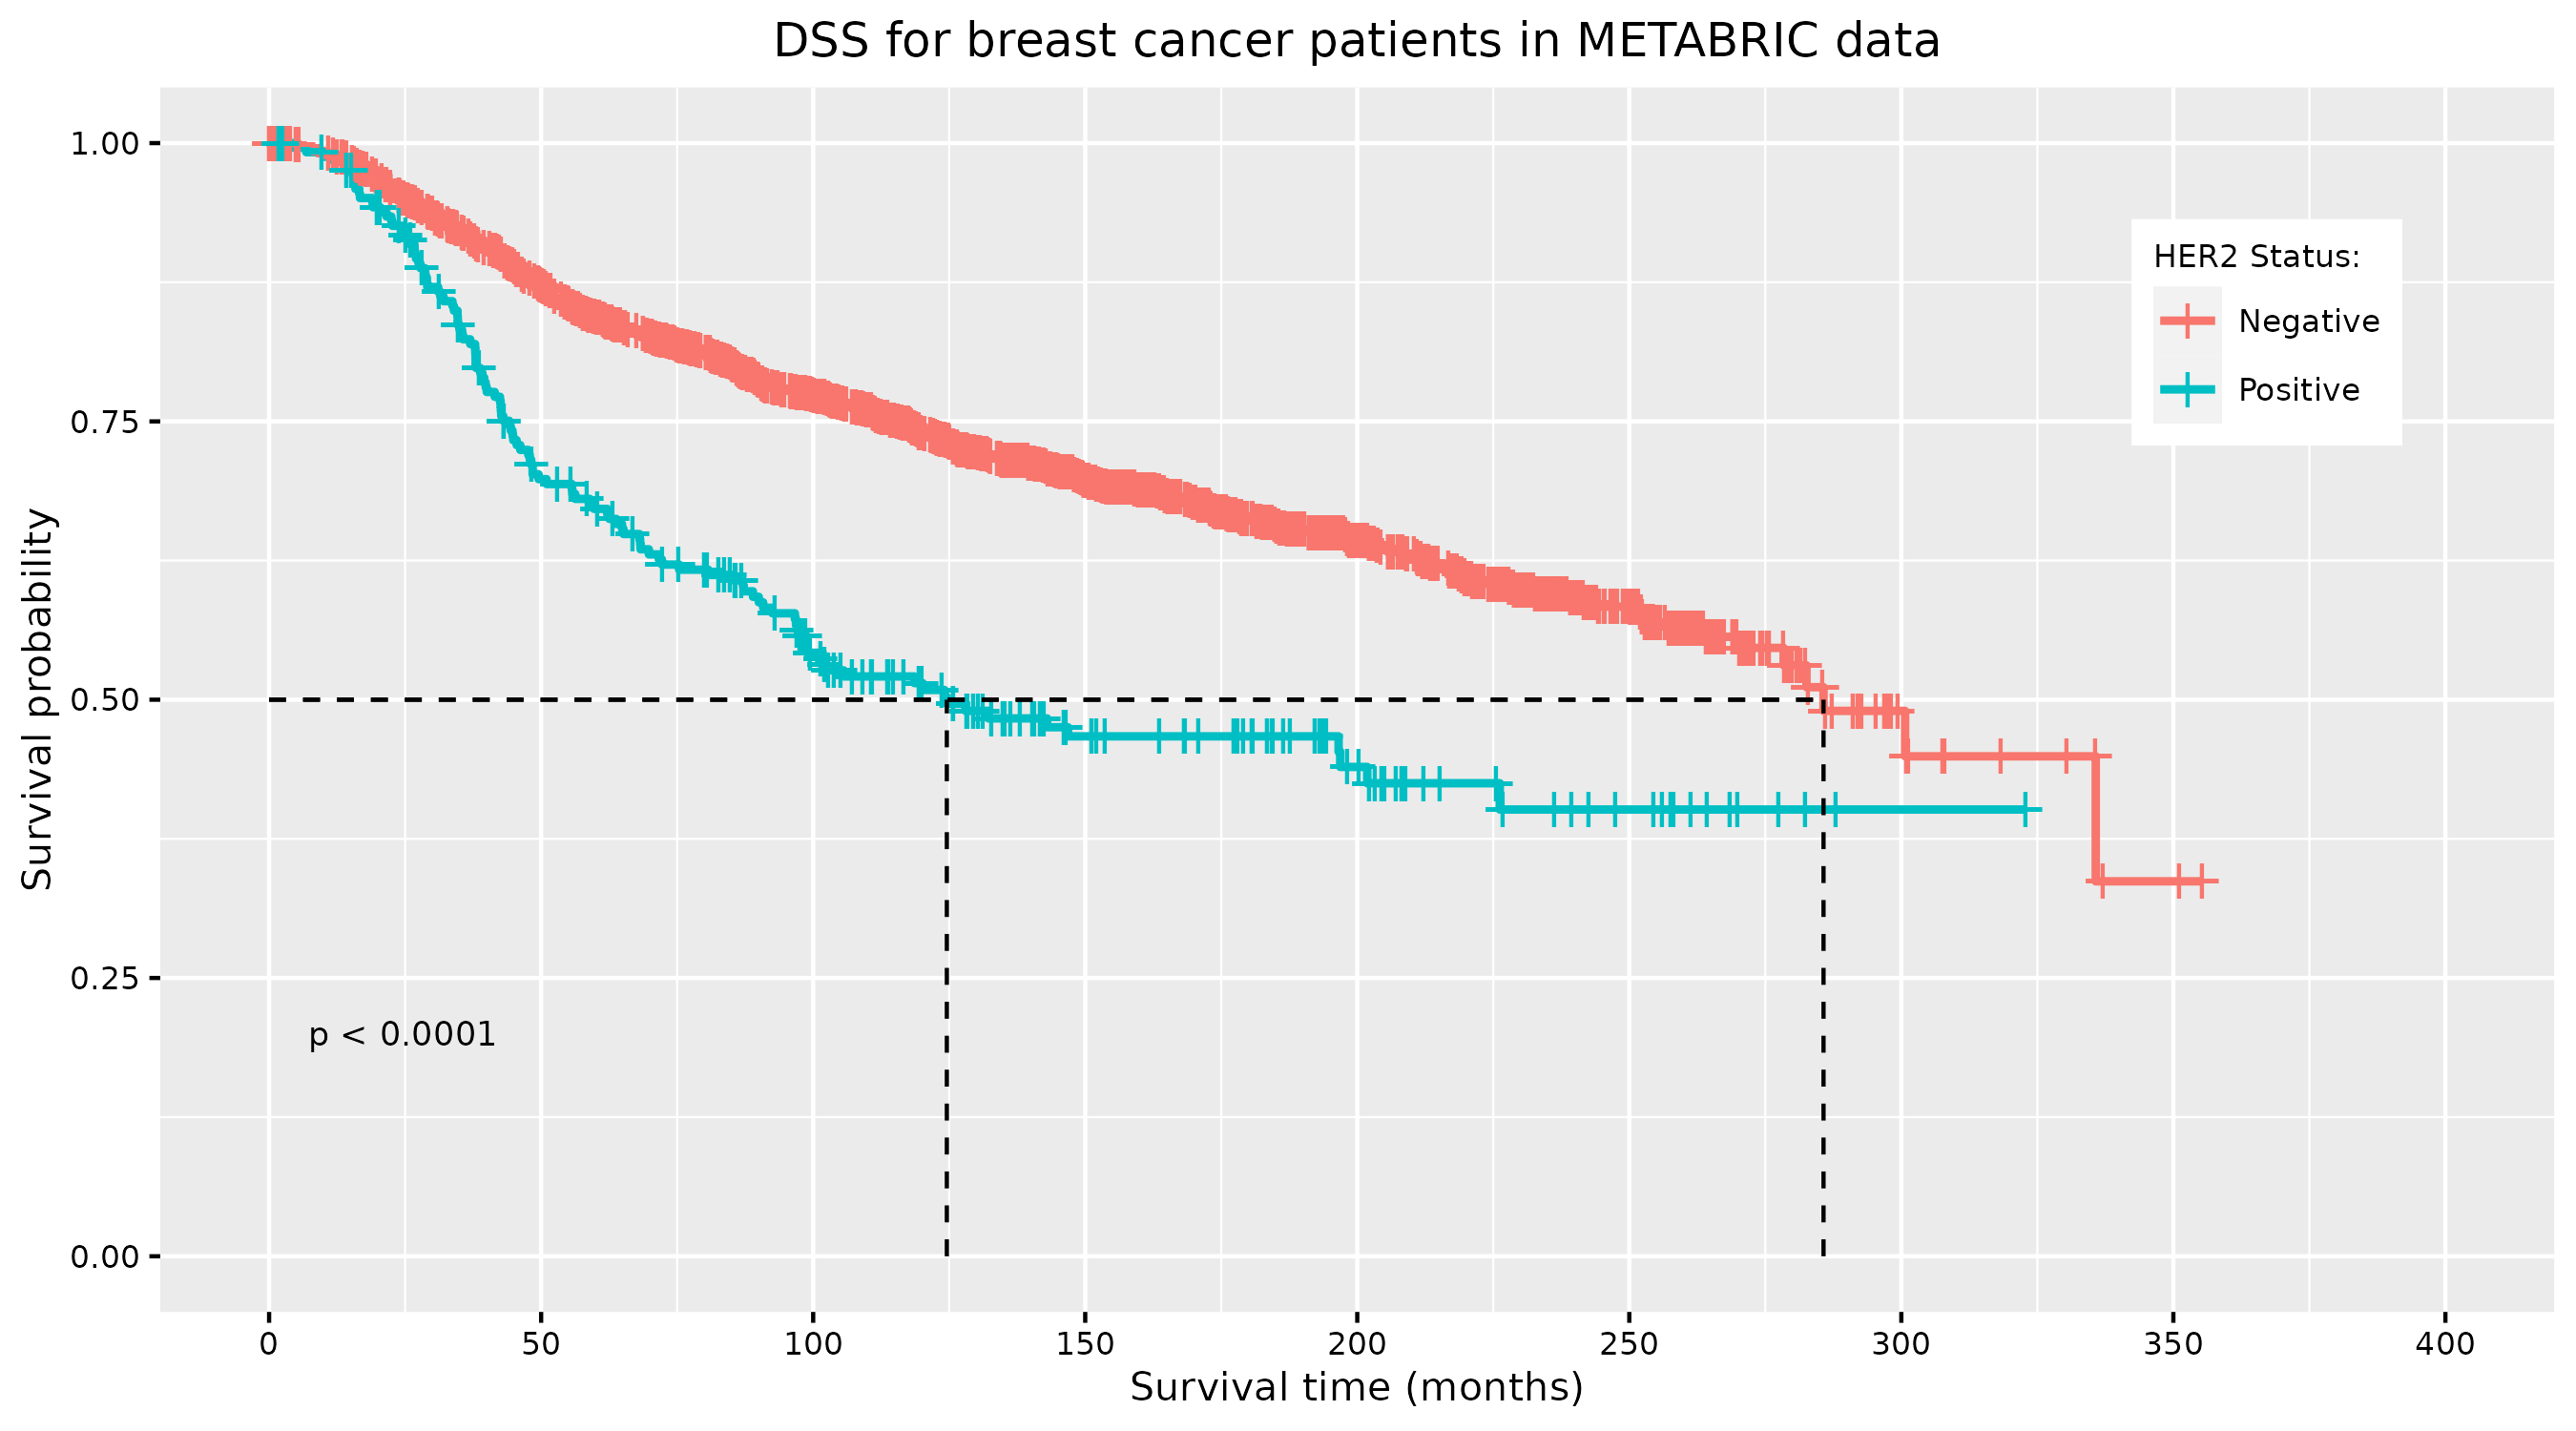
\includegraphics[width=1\textwidth]{../figures/Chapter_3/Example_Survival_Curve.png}
\caption[Kaplan-Meier plot for disease-specific survival in METABRIC patients stratified by HER2 status.]{Kaplan-Meier plot for disease-specific survival in METABRIC patients stratified by HER2 status. Lines corresponding to median disease-specific survival time for each group and the p-value associated with the log-rank test are displayed.}
\label{fig:SurvivalCurves}
\end{figure}
\vfill
\clearpage 

To determine whether two or more survival curves are significantly different from each other, a large-sample $\chi^2$ test (the log-rank test) tests the null hypothesis of no difference between the populations in the probability of an event at any time point. In Figure \ref{fig:SurvivalCurves}, the $p<0.0001$ indicates a significant difference in DSS comparing HER2- and HER2+ patients. 

\subsubsection{Recursive Partitioning Survival Trees}
Recursive partitioning techniques or tree-based methods were first developed by \cite{Morgan_Sonquist_1963} but were popularised in the 1980s following the development of the Classification and Regression Tree (CART) by Breiman et al. \citep{breiman_1984, bb_2011}. More recently, conditional inference trees (CTREE) have been developed to resolve some of the limitations of CART including overfitting and selection bias towards variables with many possible splits, i.e. continuous variables \citep{hothorn_hornik_zeileis_2006}. These non-parametric techniques are useful for identifying important predictors and structure in a dataset.  

These techniques recursively partition the data to form groups, called nodes, containing individuals with homogenous response values. The predicted response value for each node is then generally either the mean or mode dependent on whether the partitioning variable is continuous or categorical. Within the CART methodology, splits within the tree are arrived at by minimising a measure of node impurity. For categorical response variables measures of impurity may be the Gini index or information index. The Gini index denotes the probability that a random observation is misclassified when chosen randomly, while the information index relates to how much information is gained by splitting a set of data on a particular feature. For continuous response variables this measure may be the sum of squared deviations from the mean. The CTREE methodology differs in that the splits within the tree are arrived at using p-values from permutation-based significance tests.  

Using the CART or CTREE methodologies to produce predictive models has a number of advantages which are detailed below: 

\begin{enumerate}
\item No distributional assumptions are made. 
\item The predictor variables used can be continuous, interval or categorical. 
\item Robust to outliers, collinearities and heteroscedasticity. 
\item Can detect interactions and structure in a highly complex dataset. 
\item Transformations of the data do not change the structure of the tree. 
\item Can use the same variable multiple times, i.e. at different branches in the tree.
\end{enumerate}

To apply CART and CTREE methodologies available R packages include rpart \citep{therneau1997introduction} and partykit \citep{hothorn_hornik_zeileis_2006, ctree1}. 

The rpart procedure \citep{therneau1997introduction} implements many of the ideas found in CART and builds classification models (predicts a continuous value based on the predictor variables) or regression models (predicts discrete labels or categories based on the predictor variables) which can be represented as binary trees. The rpart algorithm is an iterative algorithm where the tree is built by first identifying a single variable which best splits the data into two groups. The same process is then applied separately to each sub-group, and so on recursively until the subgroups either reach a minimum size or until no improvement can be made. To split the data, rpart uses one of several measures of impurity such as the Gini index of a node and then chooses the split with maximal impurity reduction.

The CTREE procedure, applied in partykit \citep{hothorn_hornik_zeileis_2006, ctree1}, carries out variable selection and splitting in two steps, mitigating the tendency towards predictor variables with many possible splits or many missing values. Rather than employing information measures for predictor selection, CTREE applies a significance test procedure. The conditional distribution of statistics measuring the association between responses and predictor variables is responsible for the unbiased selection of variables that are measured on different scales. In addition, this algorithm applies multiple testing procedures to determine if there is no significant association between any of the predictors and the response and as such decides when the recursion should be halted. 

\subsection{CNA Metrics Stratify Luminal Breast Cancer Patients to Explain Survival Outcome}
Approximately 70\% of breast cancers are classified as Luminal A or B, characterised by increased levels of ER and PR \citep{pmid27341628}. Luminal B tumours tend to grow faster than Luminal A tumours, are of a higher grade, have a slightly worse prognosis and usually require more aggressive treatments. It has been suggested that the relationship between Luminal A and Luminal B tumours may be a continuum rather than a strict division of subtypes \citep{pmid18662380, pmid22522925, pmid27341628}. It has also been hypothesised that Luminal A tumours may evolve into Luminal B tumours as a result of stochastic acquisitions of mutations in genes associated with worse prognosis, including HER2 and tumour protein p53 (TP53) \citep{PfefferUlrich2013CGMc}. This ambiguity in Luminal classification may account for the variation that exists in DSS outcome for some Luminal A patients \citep{pmid27341628, pmid26679376, pmid30849944, pmid37253056}.

With focus and application to the Luminal METABRIC patients (n = 1,175, data downloaded from cBioPortal in 2019) we aim to explore whether the metrics of GI, specifically Absolute CNA Score, can add value in modelling OS and DSS within this group. 

\subsubsection{Preliminary Survival Analysis using Absolute CNA Score and Quartiles}
To explore estimated survival curves applying KM, the continuous Absolute CNA Score (Equation \ref{eq:CNA1}) was categorised into 4 levels: Q1, Q2, Q3, Q4. Each patient is recorded as one of these levels based on whether their Absolute CNA Score was in the first quartile (lowest GI) to fourth quartile (highest GI) relative to the observed Luminal METABRIC cohort (Figure \ref{fig:Lum_Dense}). 

KM fitted to patients stratified by the four levels of Absolute CNA Score Quartile indicate significant differences between the four estimated OS curves (log-rank test $p < 0.0001$, Figure \ref{fig:OS-Survival-Luminal}). The Absolute CNA Score Quartiles are associated with OS in Luminal breast cancer patients. Those in Absolute CNA Score Q4 (highest GI) have worse survival outcomes than patients with less GI in Absolute CNA Score Quartiles 1-3 (Q1-3). For DSS outcomes, KM fitted to patients stratified by the four levels of Absolute CNA Score Quartile indicates significant differences between the four estimated DSS curves (log-rank $p < 0.0001$, Figure \ref{fig:DSS-Survival-Luminal}). Luminal breast cancer patients in Q4 have worse DSS outcomes than patients in Q1-3. 

\begin{figure}[!h]
\centering
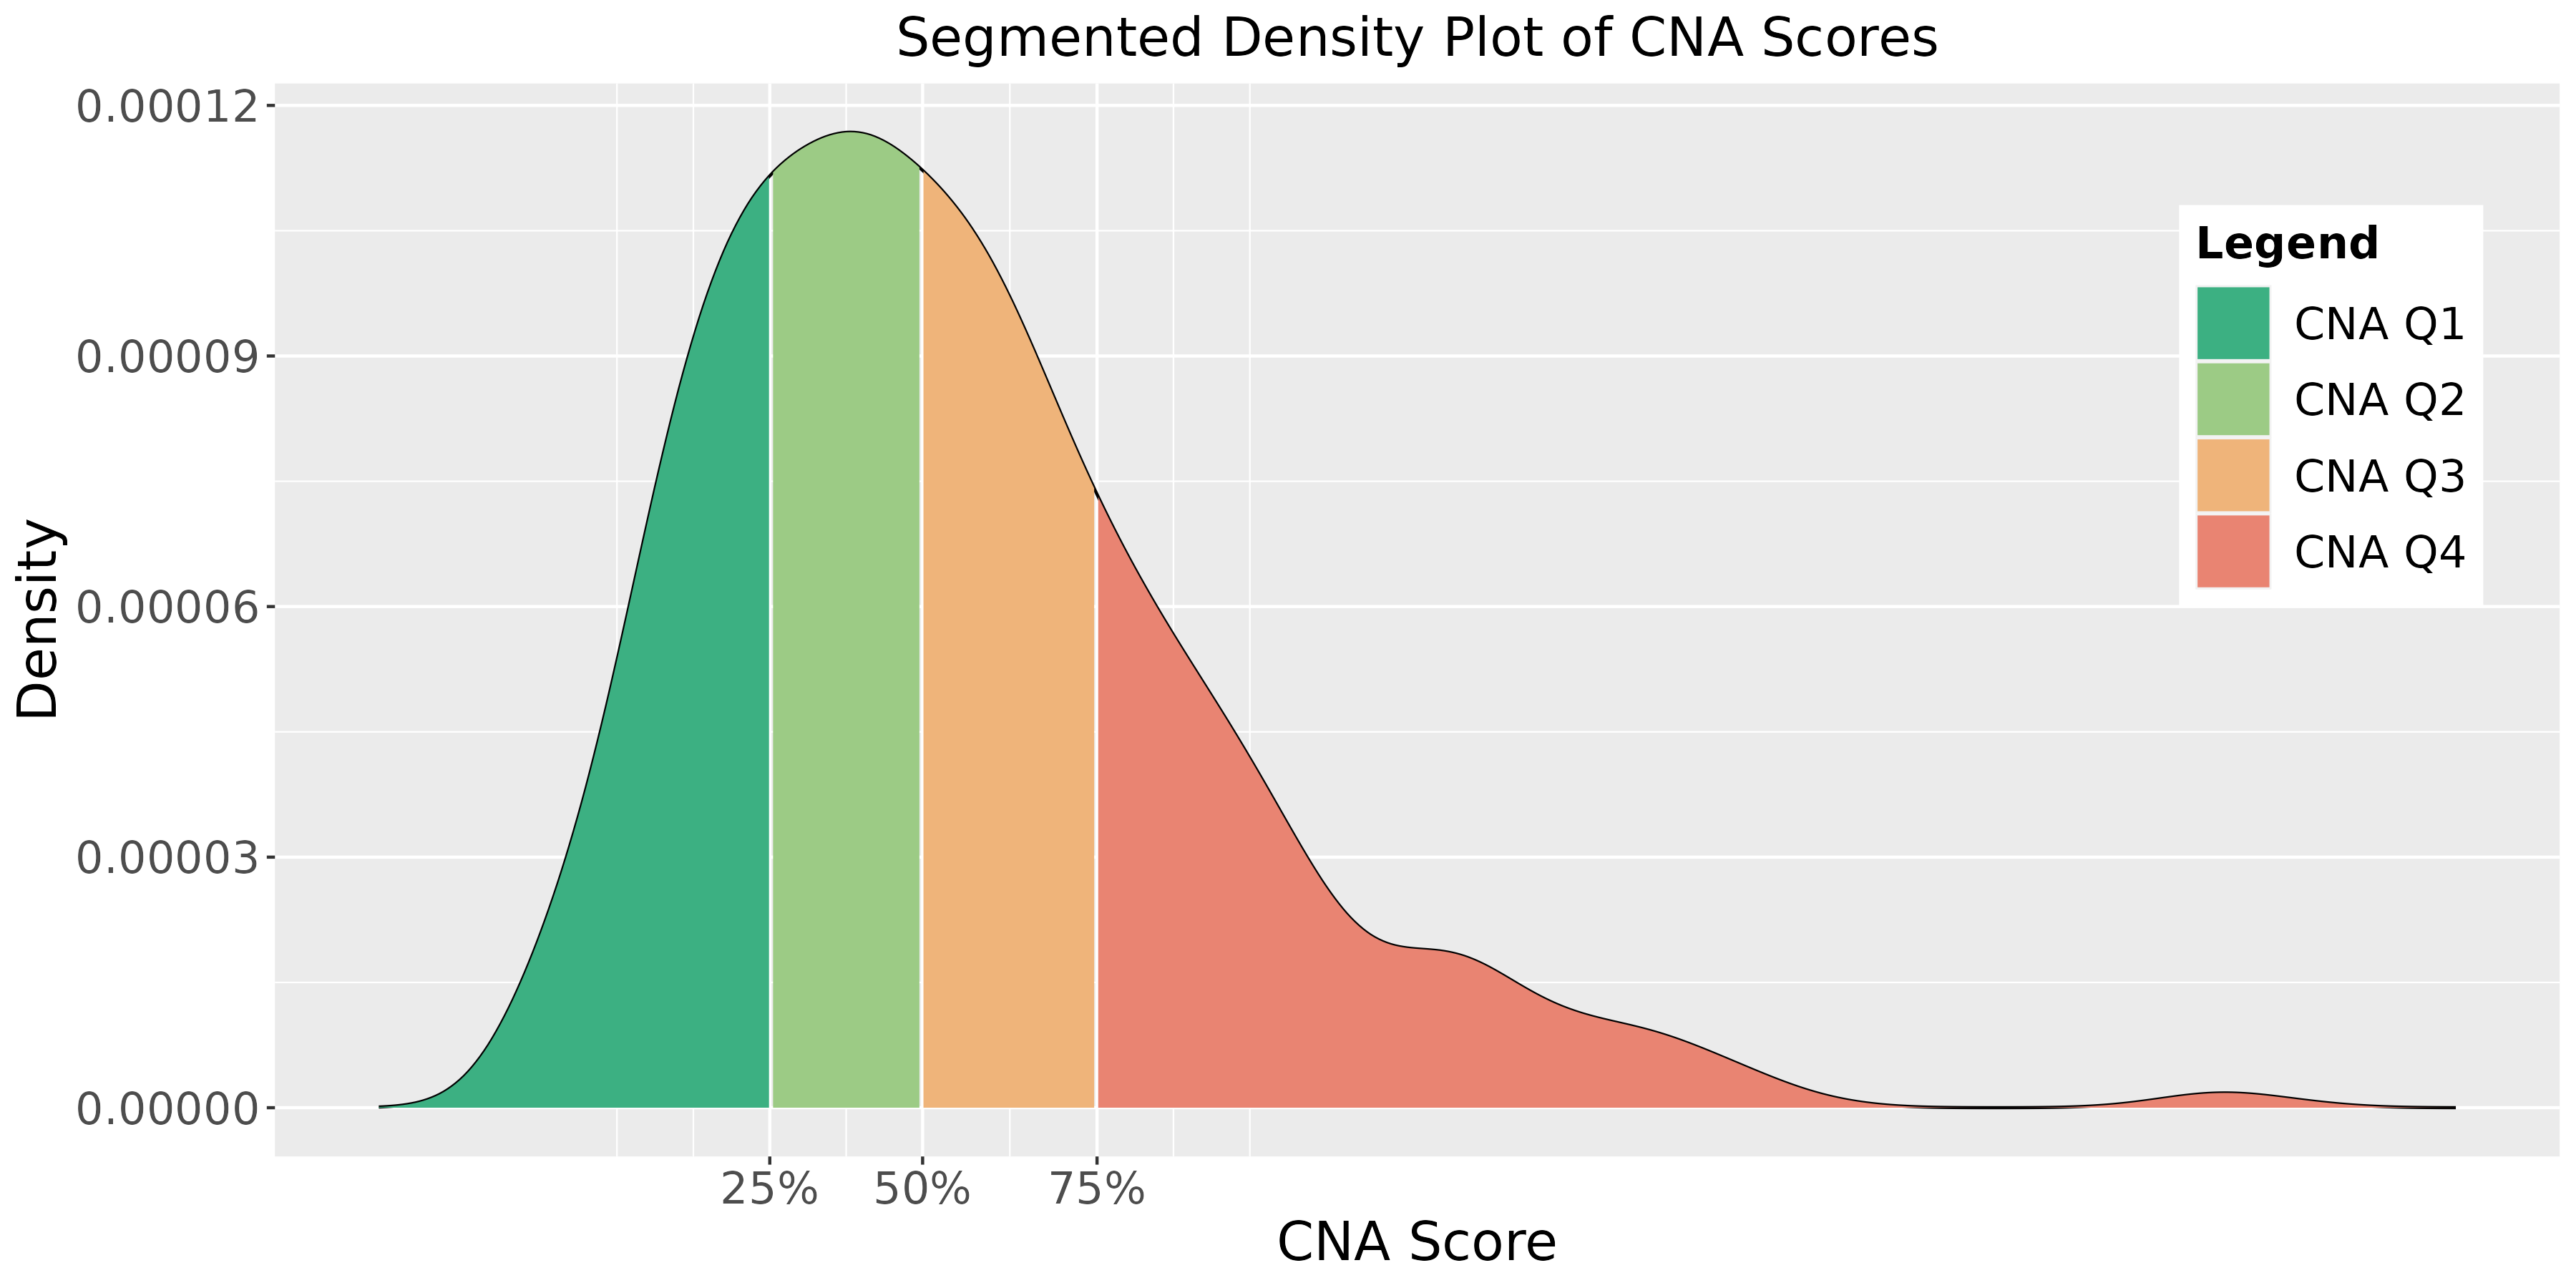
\includegraphics[width=0.98\textwidth]{../figures/Chapter_3/Luminal_AB_Score_Density.png}
\caption[Density plot of Absolute CNA Score distribution for METABRIC Luminal cases.]{Density plot of Absolute CNA Score distribution for METABRIC Luminal cases. Absolute CNA Score Quartiles 1-4 indicated by legend colours.}
\label{fig:Lum_Dense}
\end{figure}

\begin{figure}[!h]
\centering
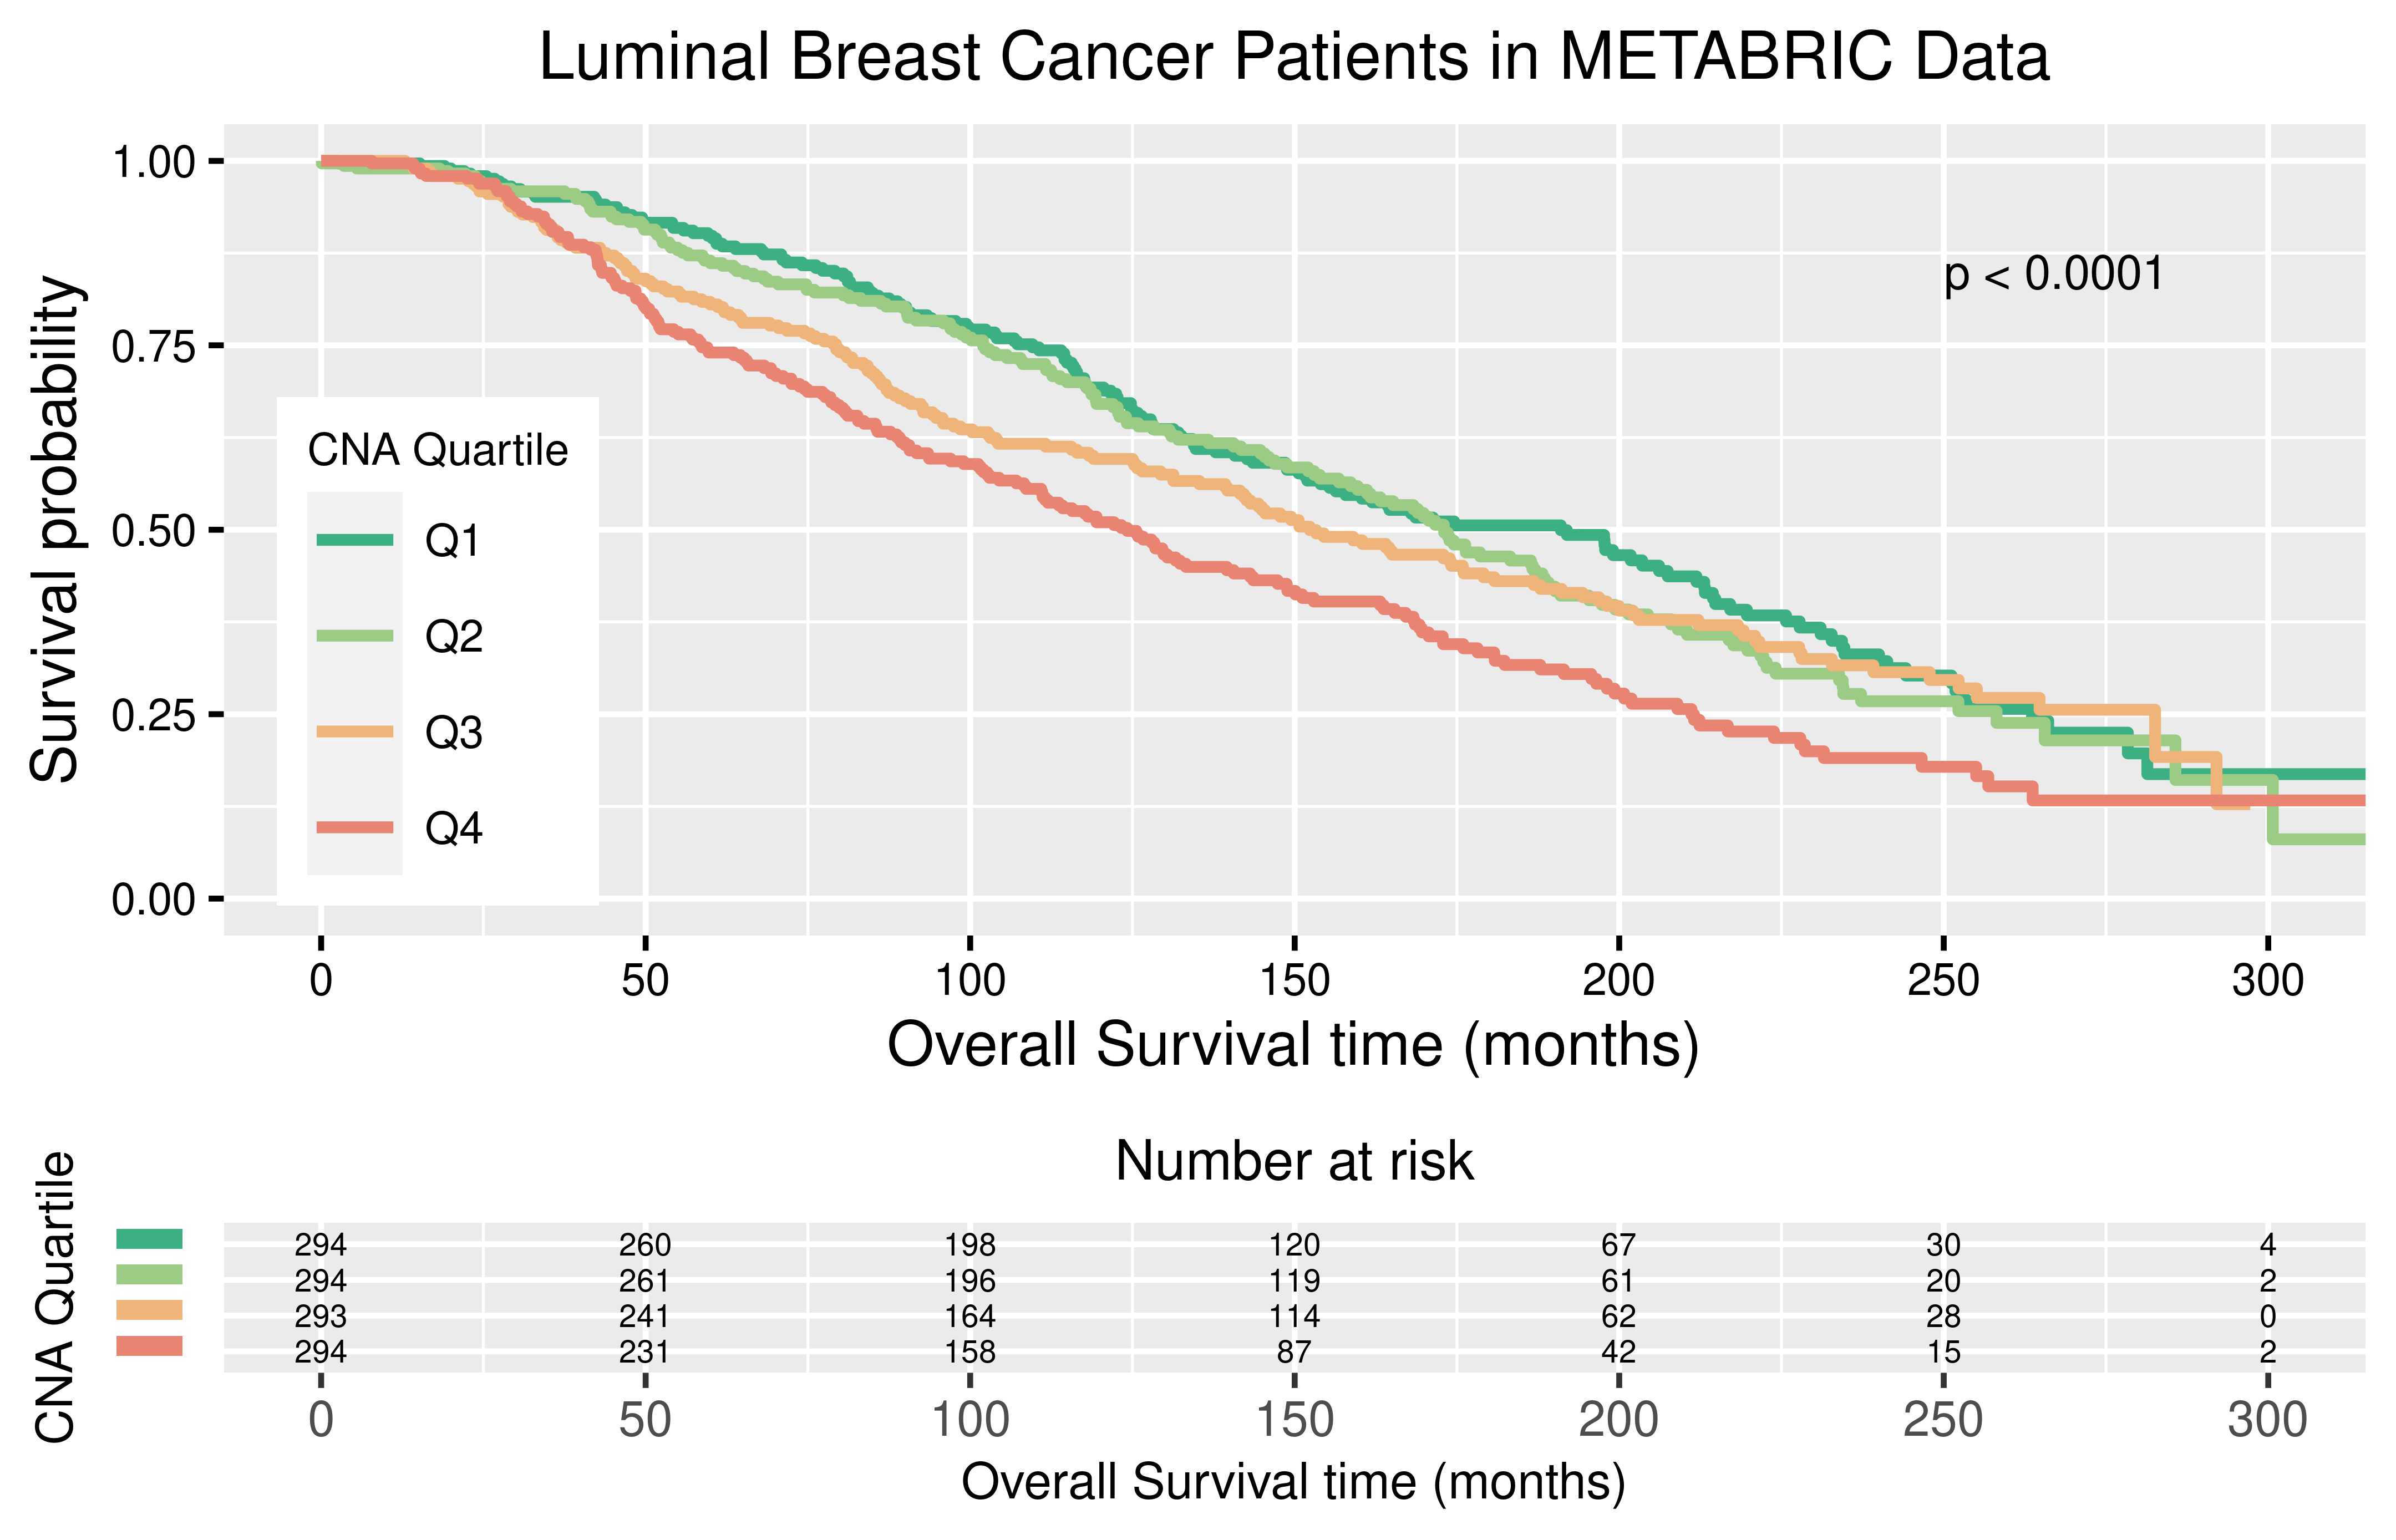
\includegraphics[width=0.98\textwidth]{../figures/Chapter_3/Luminal_AB_Score_OS.png}
\caption[Kaplan-Meier plot for overall survival for METABRIC Luminal breast cancer patients in each Absolute CNA Score Quartile.]{Kaplan-Meier plot for overall survival for METABRIC Luminal breast cancer patients in each Absolute CNA Score Quartile. The p-value associated with the log-rank test and a risk table displaying the number of patients at risk at each time interval is displayed.}
\label{fig:OS-Survival-Luminal}
\end{figure}


\begin{figure}[!h]
\centering
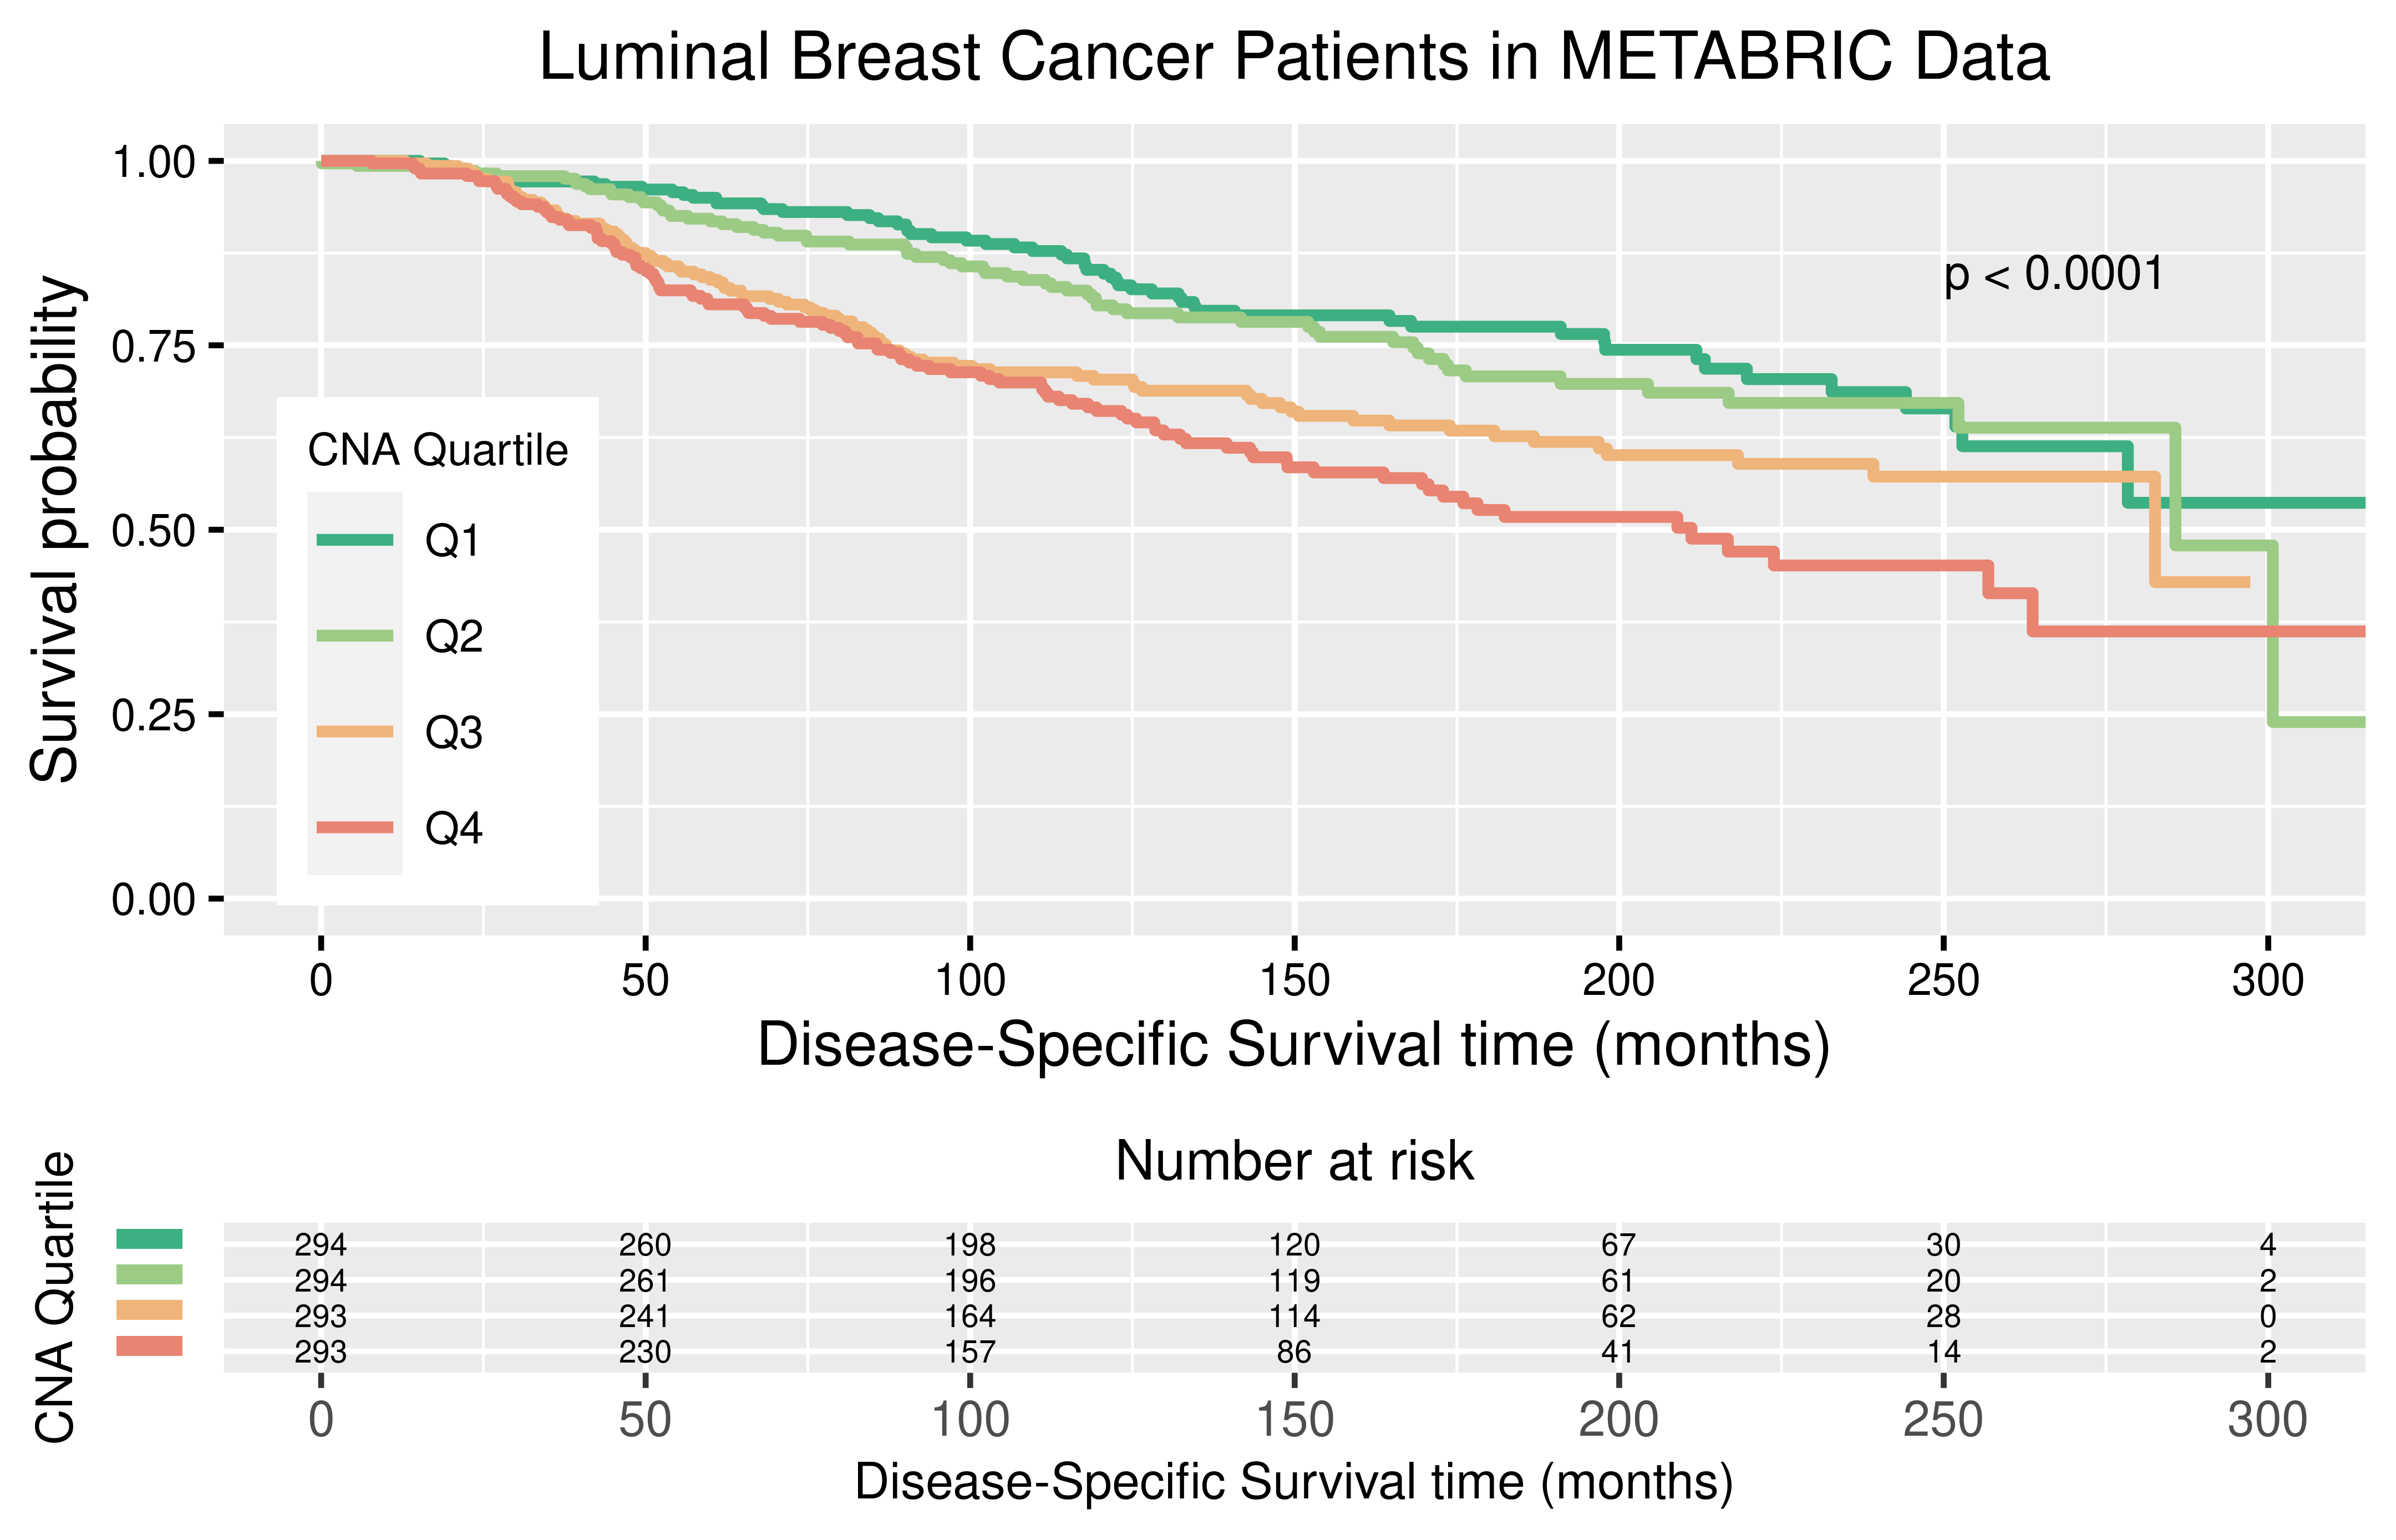
\includegraphics[width=0.98\textwidth]{../figures/Chapter_3/Luminal_AB_Score_DSS.png}
\caption[Kaplan-Meier plot for disease-specific survival for METABRIC Luminal breast cancer patients in each Absolute CNA Score Quartile.]{Kaplan-Meier plot for disease-specific survival for METABRIC Luminal breast cancer patients in each Absolute CNA Score Quartile. The p-value associated with the log-rank test and a risk table displaying the number of patients at risk at each time interval is displayed.}
\label{fig:DSS-Survival-Luminal}
\end{figure}

To maintain the information from the uncategorised, quantitative measure of Absolute CNA Score, univariate Cox models were fitted for OS and DSS. The results obtained indicate that the Absolute CNA Score is associated with both OS (Hazard Ratio (HR) = 1.00 [1.00-1.00], $p < 0.001$) and DSS (HR = 1.00 [1.00-1.00], $p < 0.0001$).

\subsubsection{Analysis of Potential Confounding Variables and Multivariable Cox Models}
Having observed that Absolute CNA Score can independently help stratify Luminal patients into groups of similar survival outcome, it is important to assess whether Absolute CNA Score can add value in combination with other biomarkers. KM plots and univariate Cox models were used to determine if any of the 23 available clinical variables (list in Appendix A) were associated with survival outcome. It was found that 19 of the clinical variables considered were associated with OS and 18 were associated with DSS (Tables \ref{tab:Surv_Tests_OS} and \ref{tab:Surv_Tests_DSS}). The clinical variables found to be significant within the univariate analysis were examined for possible associations with the Absolute CNA Scores and Absolute CNA Score Quartiles, applying tests such as the $\chi^2$ test, Fisher’s exact test, Kruskal-Wallis test and Pearson's correlation, as appropriate to the variable type. These tests indicated that the Absolute CNA Scores and CNA Score Quartiles were significantly associated with a number of clinical variables (Tables \ref{tab:Assoc_Tests_S} and \ref{tab:Assoc_Tests_Q}).

Since highly correlated predictors may lead to unreliable and unstable estimates of regression coefficients \citep{Keith_2019}, a refined selection of variables were considered based on understanding of the clinical definition of the variable, e.g. HER2 Status and HER2 SNP6 use different methods to capture similar information (discussed further in \cite{King_2021}). Eight candidate clinical predictors remained: PAM50 subtype, histological grade, tumour size, number of lymph nodes positive, age, HER2 status, PR status and histological subtype. These eight candidate clinical predictors were considered along with either the Absolute CNA Score or Absolute CNA Score Quartile variable in multivariable CPH models for OSS and DSS. Under the assumption of proportional hazards, the results indicated that the Absolute CNA Score metric was significantly associated with the outcome in a model for DSS along with six clinical predictors: PAM50 subtype, histological grade, tumour size, number of positive lymph nodes, age at diagnosis, and HER2 status, both using the categorical CNA Score Quartiles (Table \ref{table_mcm}) and the original continuous Absolute CNA Scores (Table \ref{table_mcms}). 

\vfill
\begin{table}[!h]
\caption[Overall survival univariate Cox models for each clinical variable.]{Overall survival univariate Cox models for each clinical variable. Likelihood ratio test (LRT) and Wald test p-values and Benjamini-Hochberg adjusted p-values are displayed.}
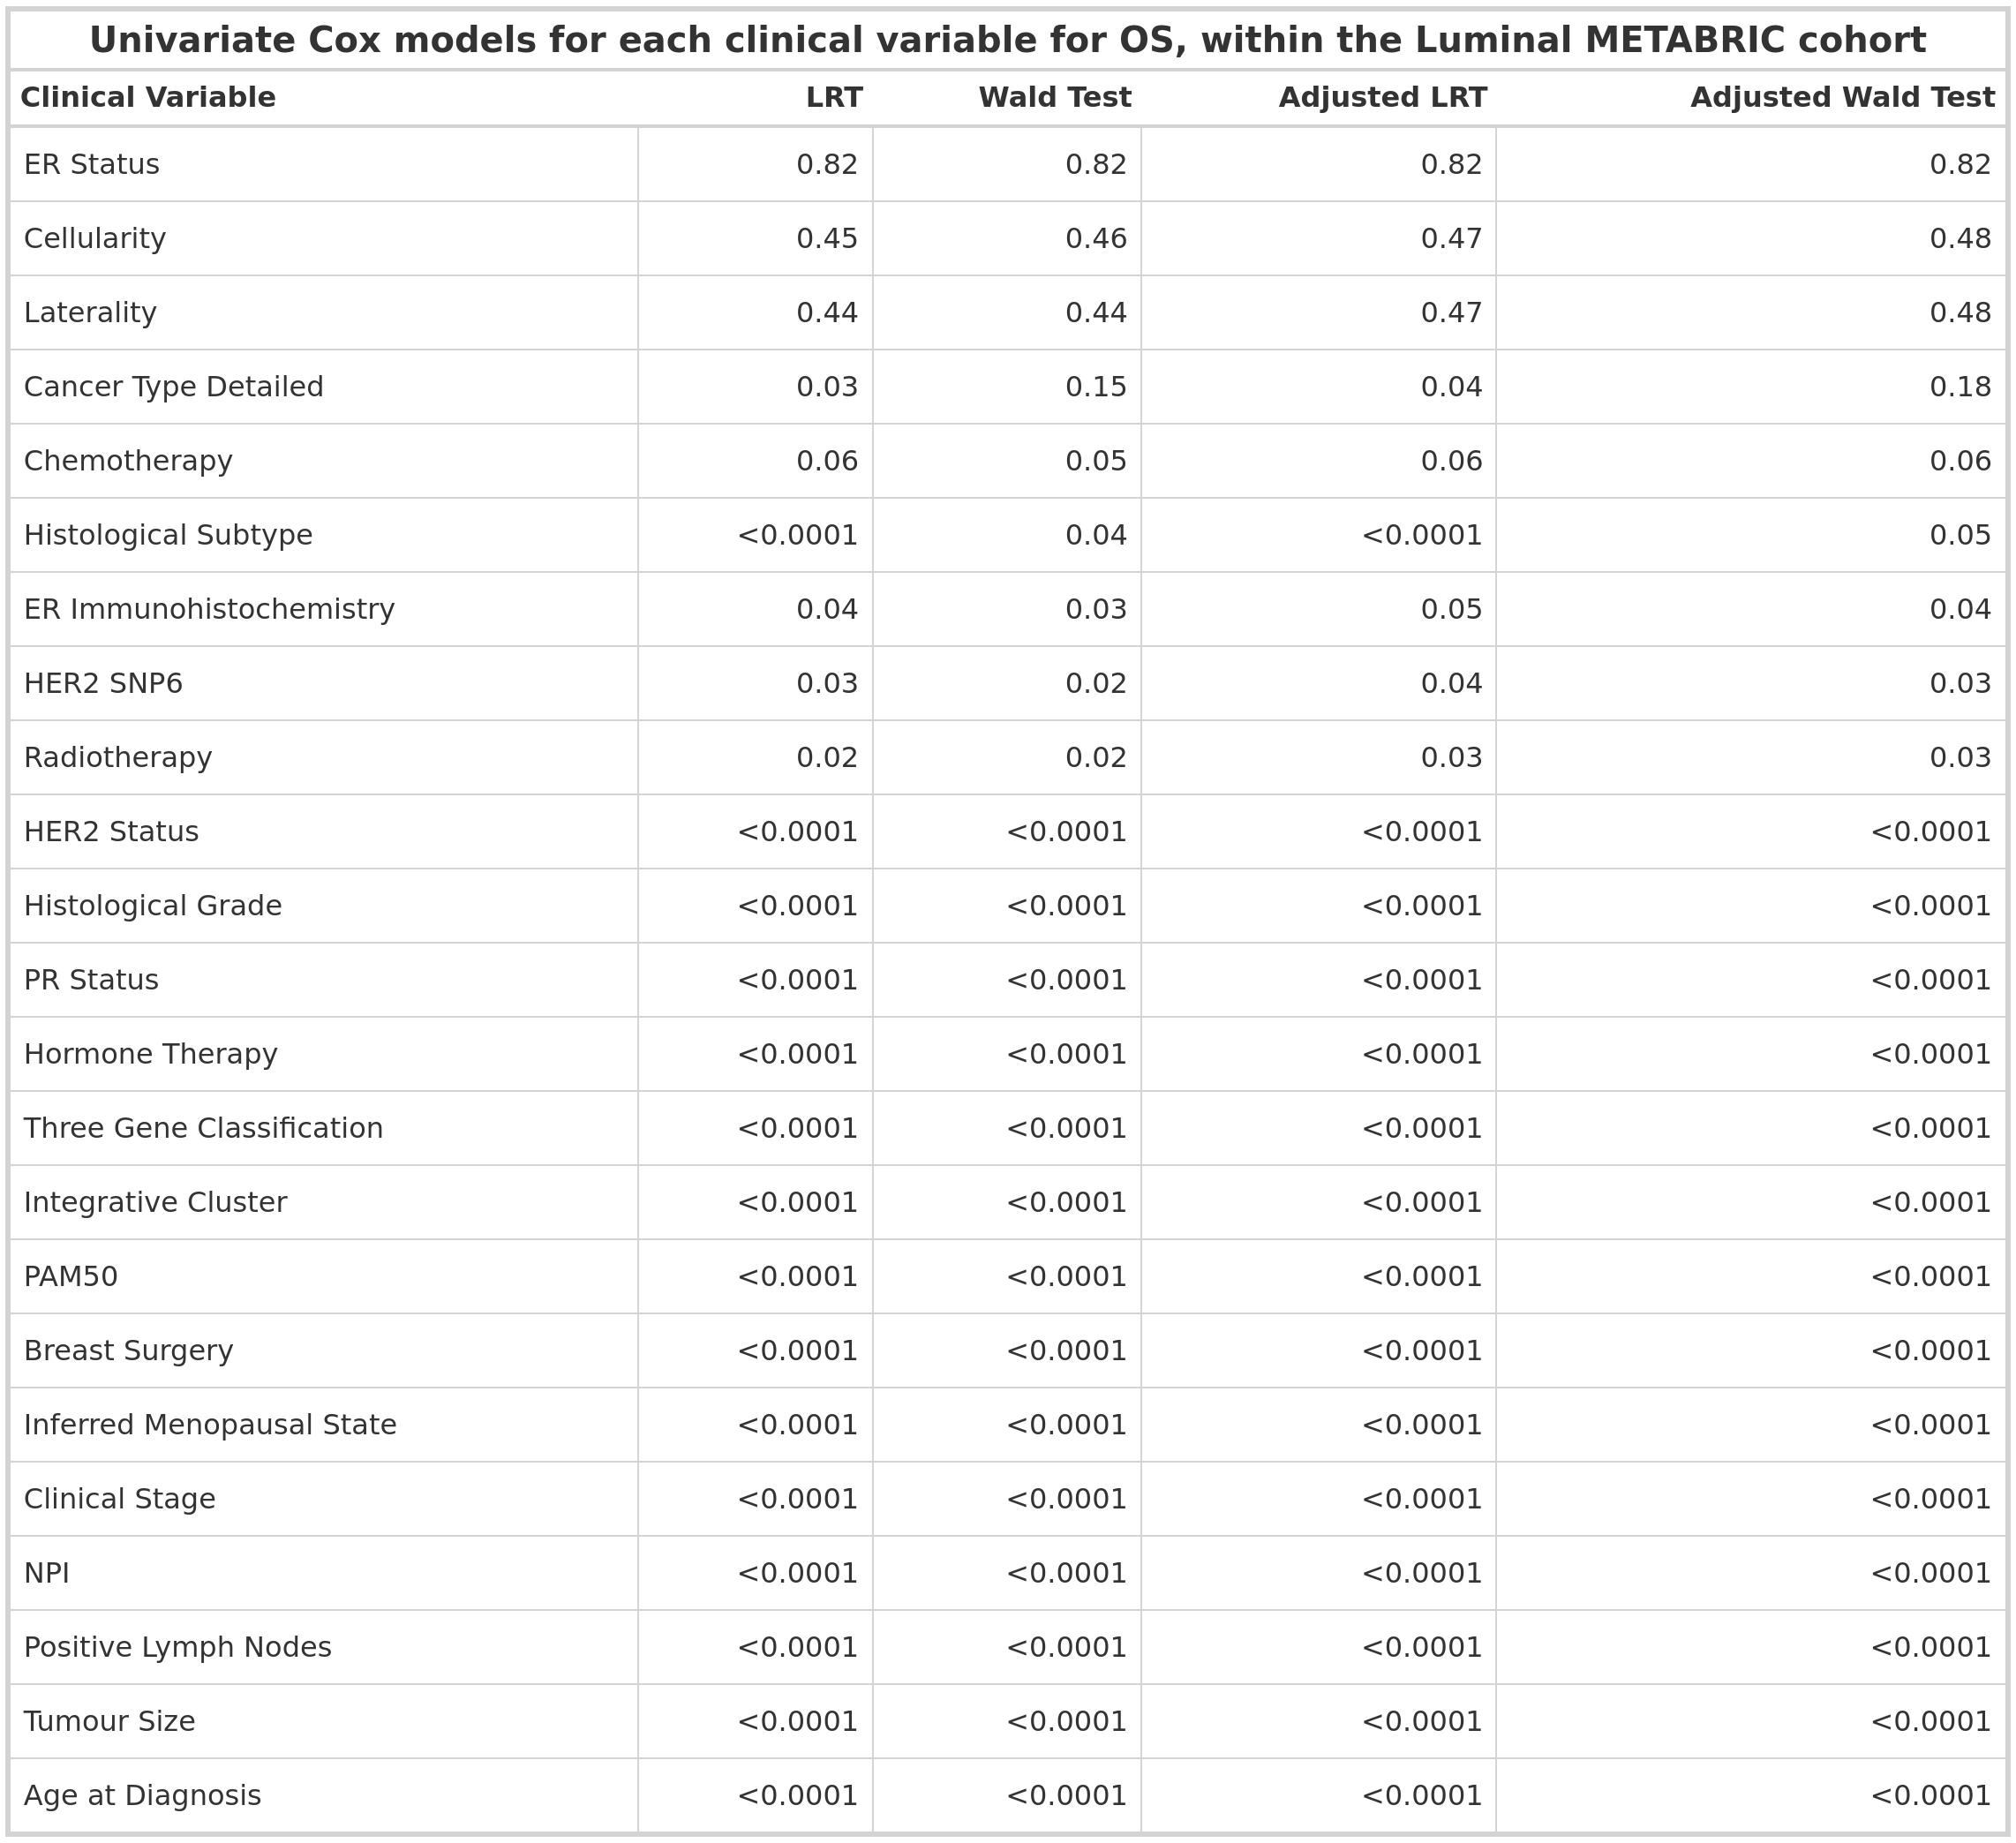
\includegraphics[width=0.98\textwidth]{../tables/Chapter_3/Luminal_Survival_Association_OS.png}
\label{tab:Surv_Tests_OS}
\end{table}
\vfill
\clearpage
\begin{table}[!ht]
\caption[Disease-specific survival univariate Cox models for each clinical variable.]{Disease-specific survival univariate Cox models for each clinical variable. Likelihood ratio test (LRT) and Wald test p-values and Benjamini-Hochberg adjusted p-values are displayed.}
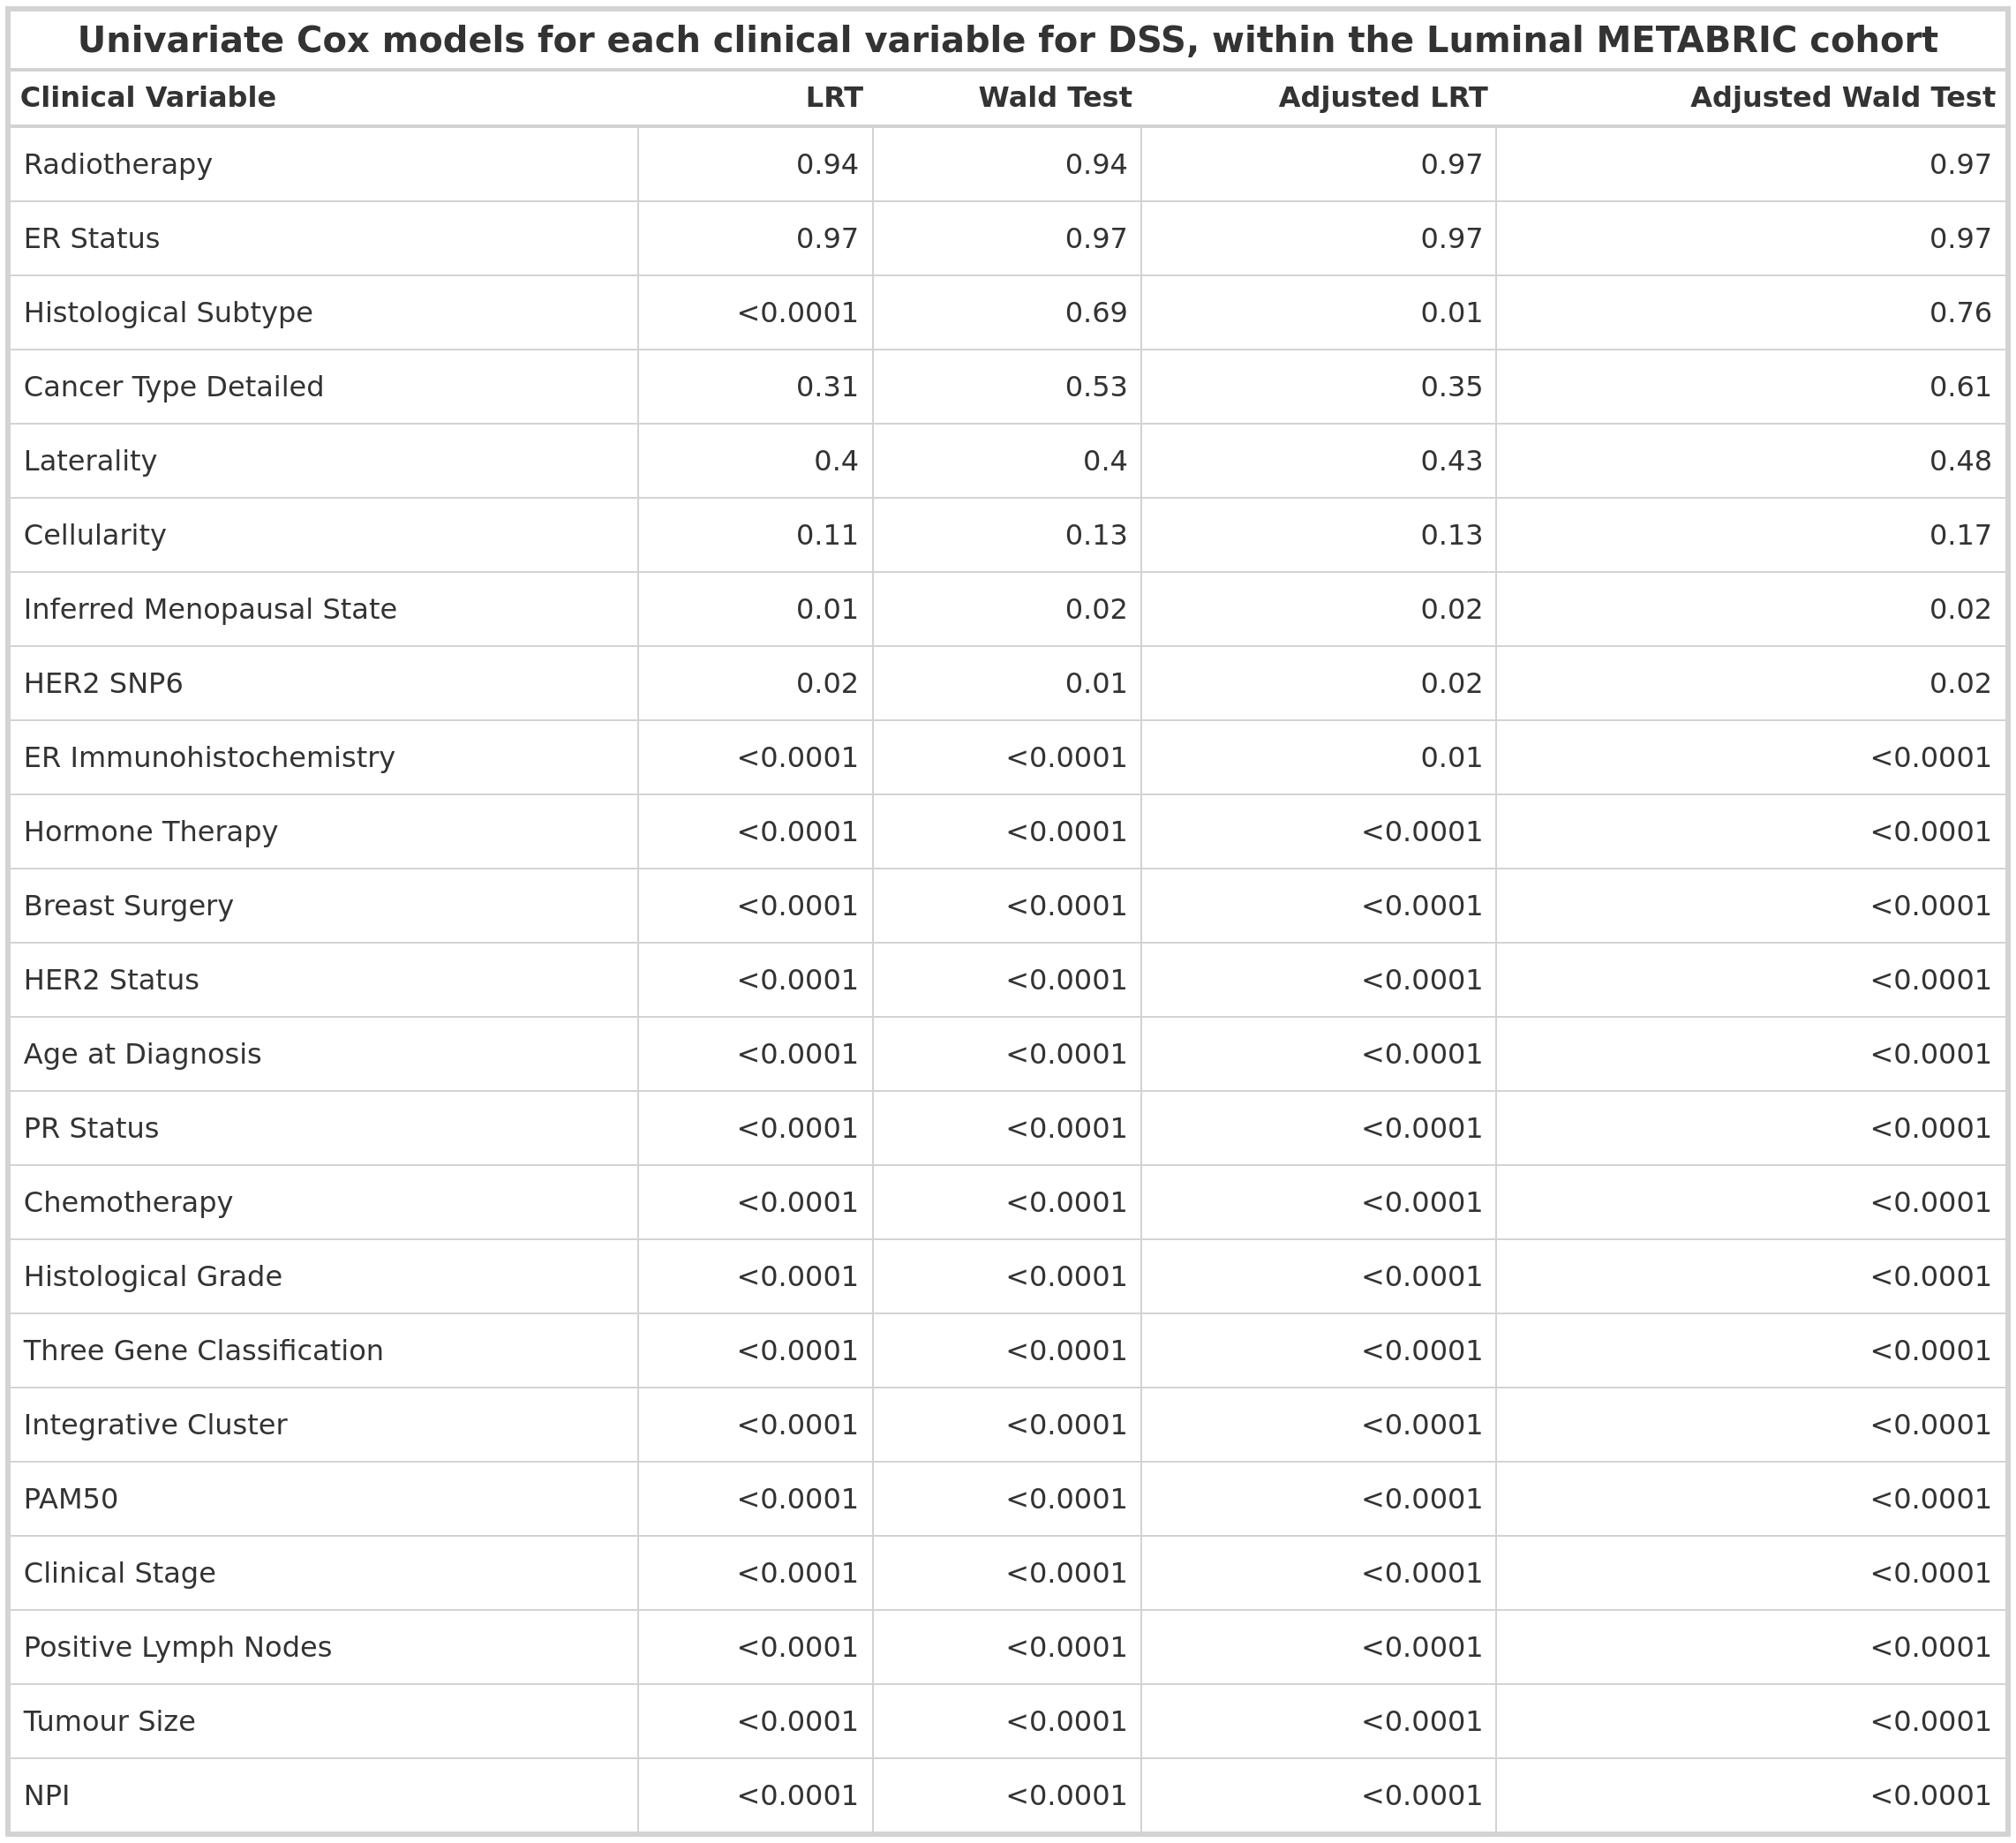
\includegraphics[width=0.98\textwidth]{../tables/Chapter_3/Luminal_Survival_Association_DSS.png}
\label{tab:Surv_Tests_DSS}
\end{table}

As the focus and application here is only within Luminal cancers, PAM50 subtype has only two levels Luminal A and Luminal B. In the fitted models an indicator variable assumes the reference group to be Luminal A, and the estimated effect using this indicator is for Luminal B relative to Luminal A. In the model using Absolute CNA Scores the reference group is Luminal A, histological grade 1, HER2-negative patients (Table \ref{table_mcms}). For Luminal A patients, Absolute CNA Score is associated with DSS (HR = 1.00 [1.00-1.00], $p < 0.001$). For Luminal B patients, the effect of Absolute CNA Score on DSS is estimated by fitting interaction effects between Absolute CNA Score and PAM50 subtype. This indicates that the association between Absolute CNA Score is significantly different for Luminal B patients compared to Luminal A patients (HR = 1.00 [0.99-1.00], $p < 0.012$). Setting Luminal B as the reference group indicates that for Luminal B patients, Absolute CNA Score is not associated with DSS.  

In the model using Absolute CNA Score Quartiles the reference group is Luminal A, histological grade 1, HER2-negative patients with Absolute CNA Scores with lowest GI level, Absolute CNA Score Q1 (Table \ref{table_mcm}). Comparing Absolute CNA Score Q4 to CNA Q1, within Luminal A patients, shows a significant increased risk in DSS (HR = 2.32 [1.36-3.94], $p = 0.002$). Comparing Absolute CNA Score Q3 to Absolute CNA Score Q1, within Luminal A patients, shows a significant increased risk in DSS (HR = 2.15 [1.33-3.49], $p = 0.002$). There was no evidence of a significant effect on risk comparing Absolute CNA Score Q2 Luminal A patients to Absolute CNA Score Q1 Luminal A patients (HR = 1.37 [0.83 - 2.27], $p = 0.219$). For Luminal B patients, the effect of Absolute CNA Score Quartile on DSS differs in comparison to Luminal A patients estimated by fitting interaction effects between Absolute CNA Score Quartiles and PAM50 subtype, the effect is a reduction in the estimated difference comparing Absolute CNA Score Quartile within Luminal B. 


\begin{table}[!htb]
\caption[Association tests between CNA Score and selected clinical variables.]{Association tests between CNA Score and selected clinical variables. Kruskal-Wallis and Pearson's Correlation p-values and Benjamini-Hochberg adjusted p-values are displayed.}
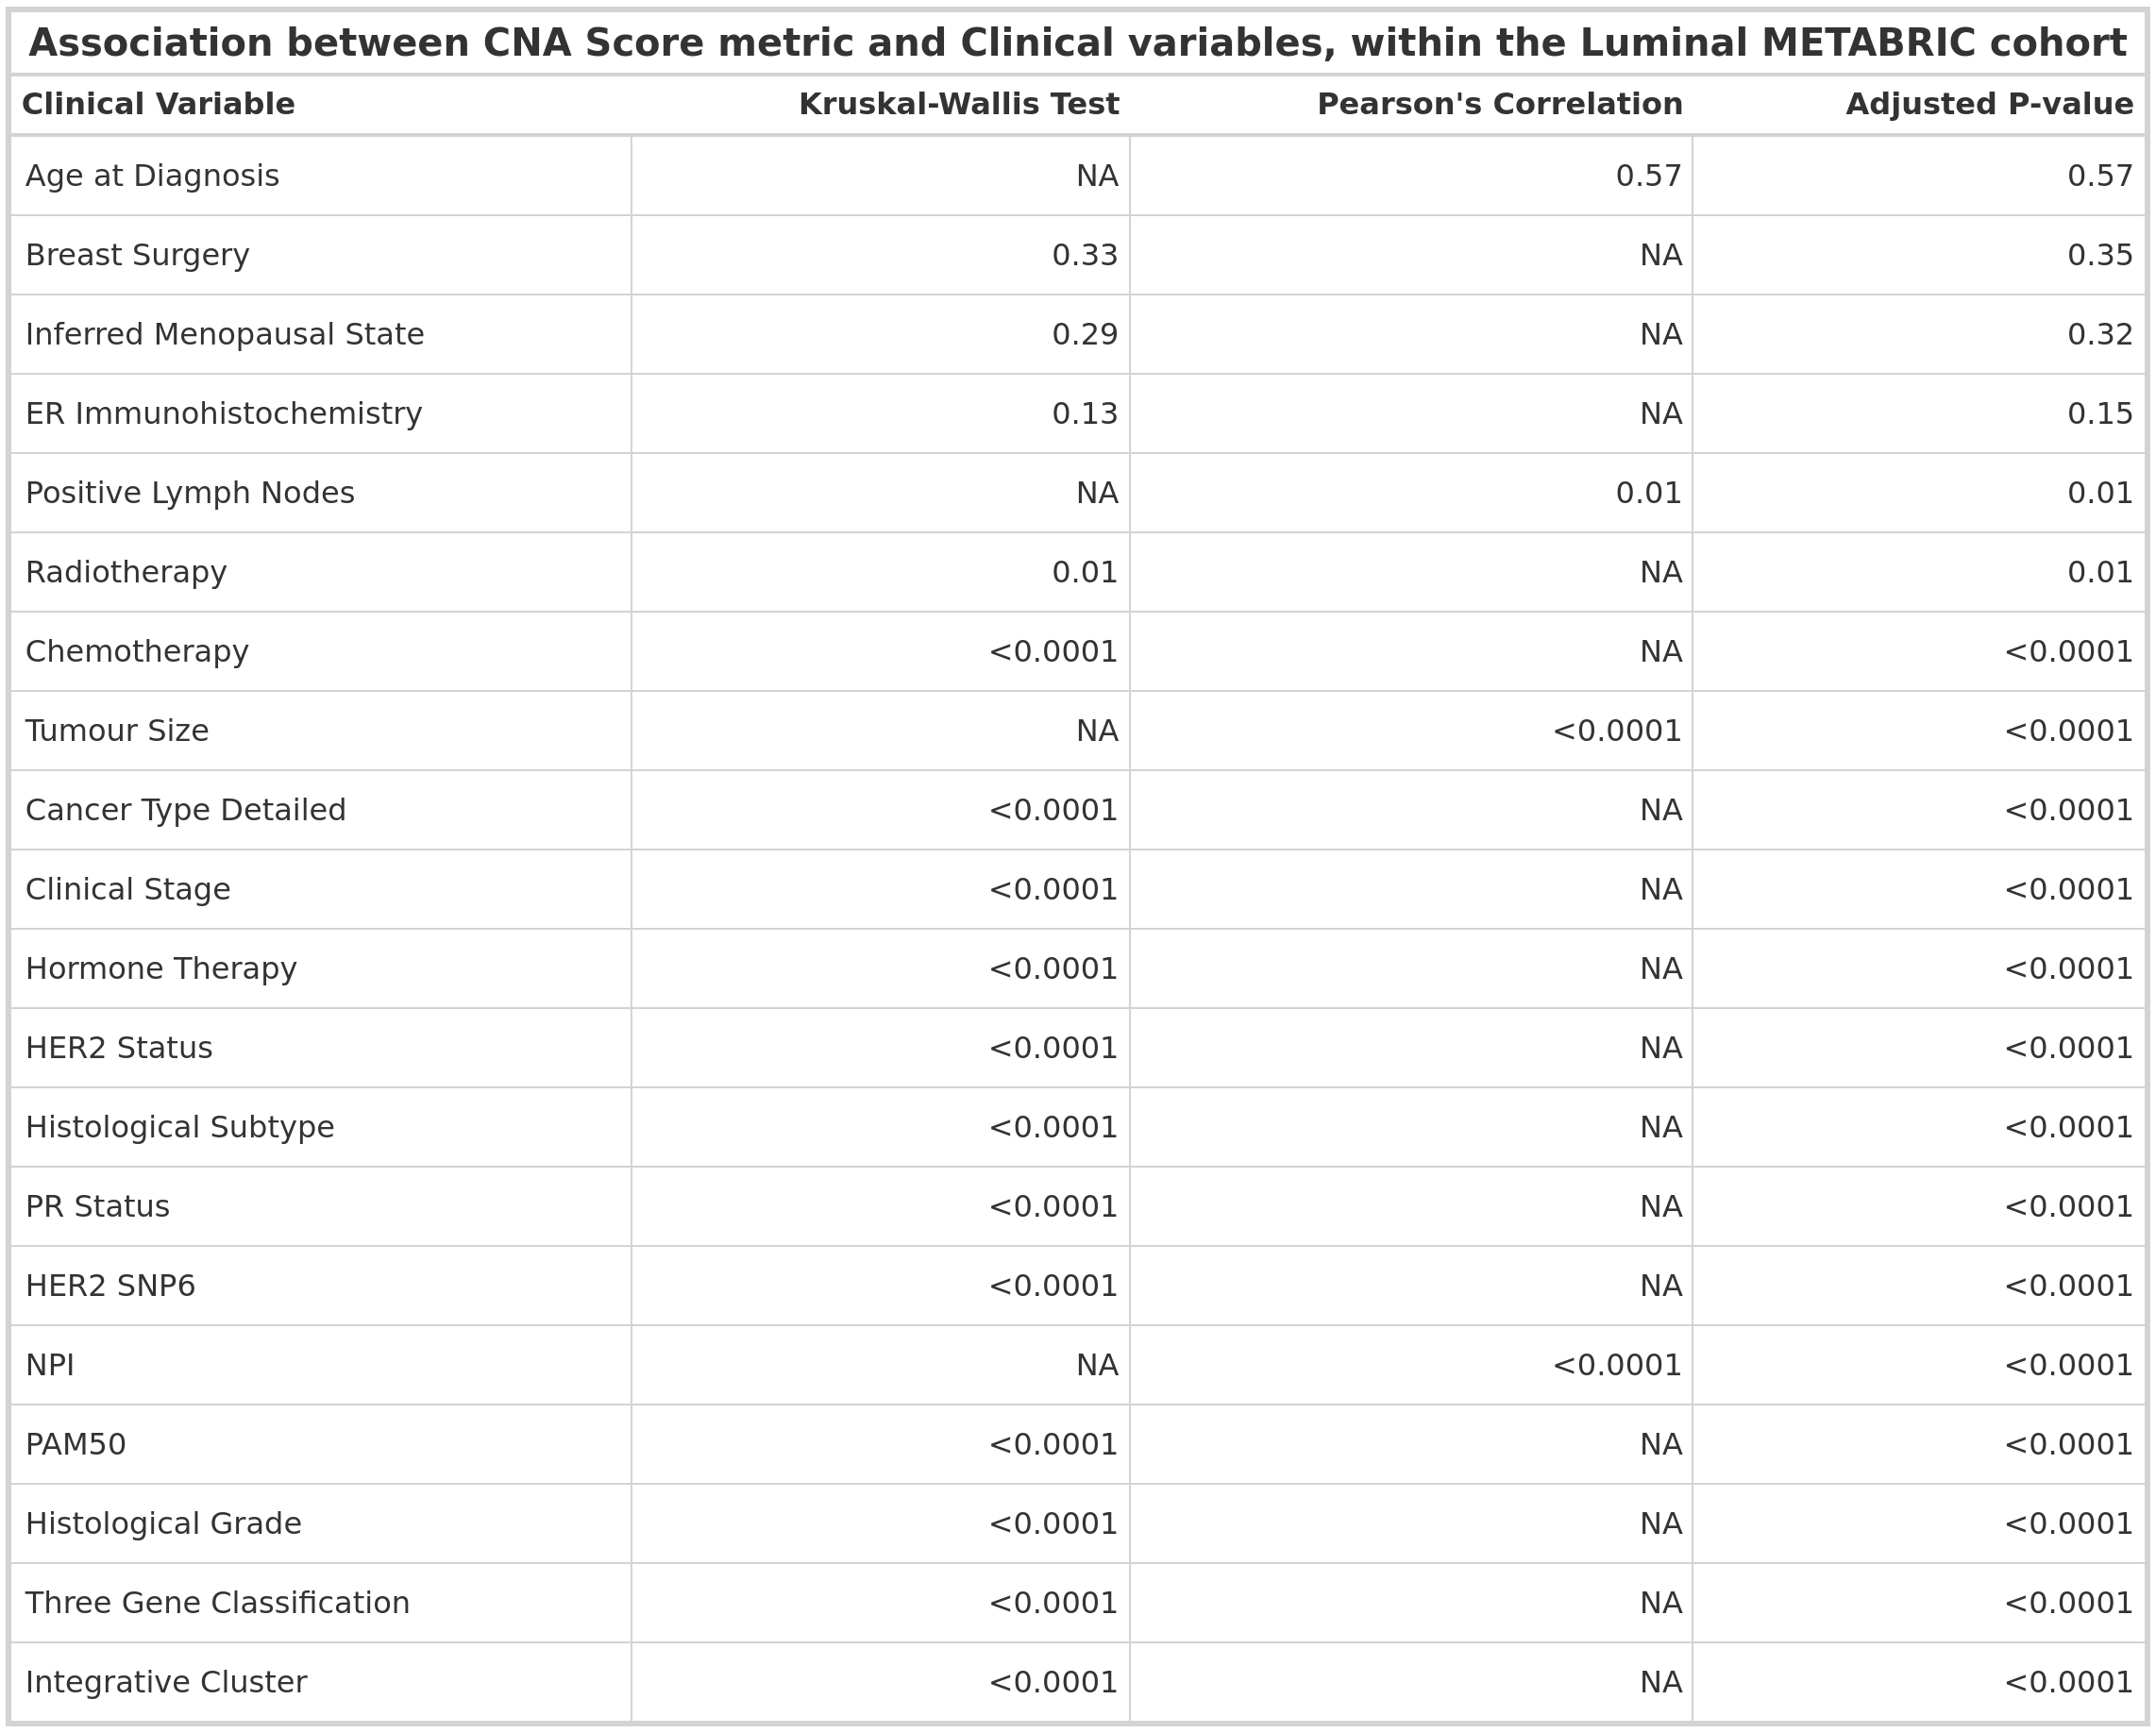
\includegraphics[width=0.98\textwidth]{../tables/Chapter_3/CNA_Score_Clin_Association.png}
\label{tab:Assoc_Tests_S}
\end{table}

\begin{table}[!htb]
\caption[Association tests between CNA Quartiles and selected clinical variables.]{Association tests between CNA Quartiles and selected clinical variables. $\chi^2$, Fisher's Exact and Kruskal-Wallis test p-values and Benjamini-Hochberg adjusted p-values are displayed.}
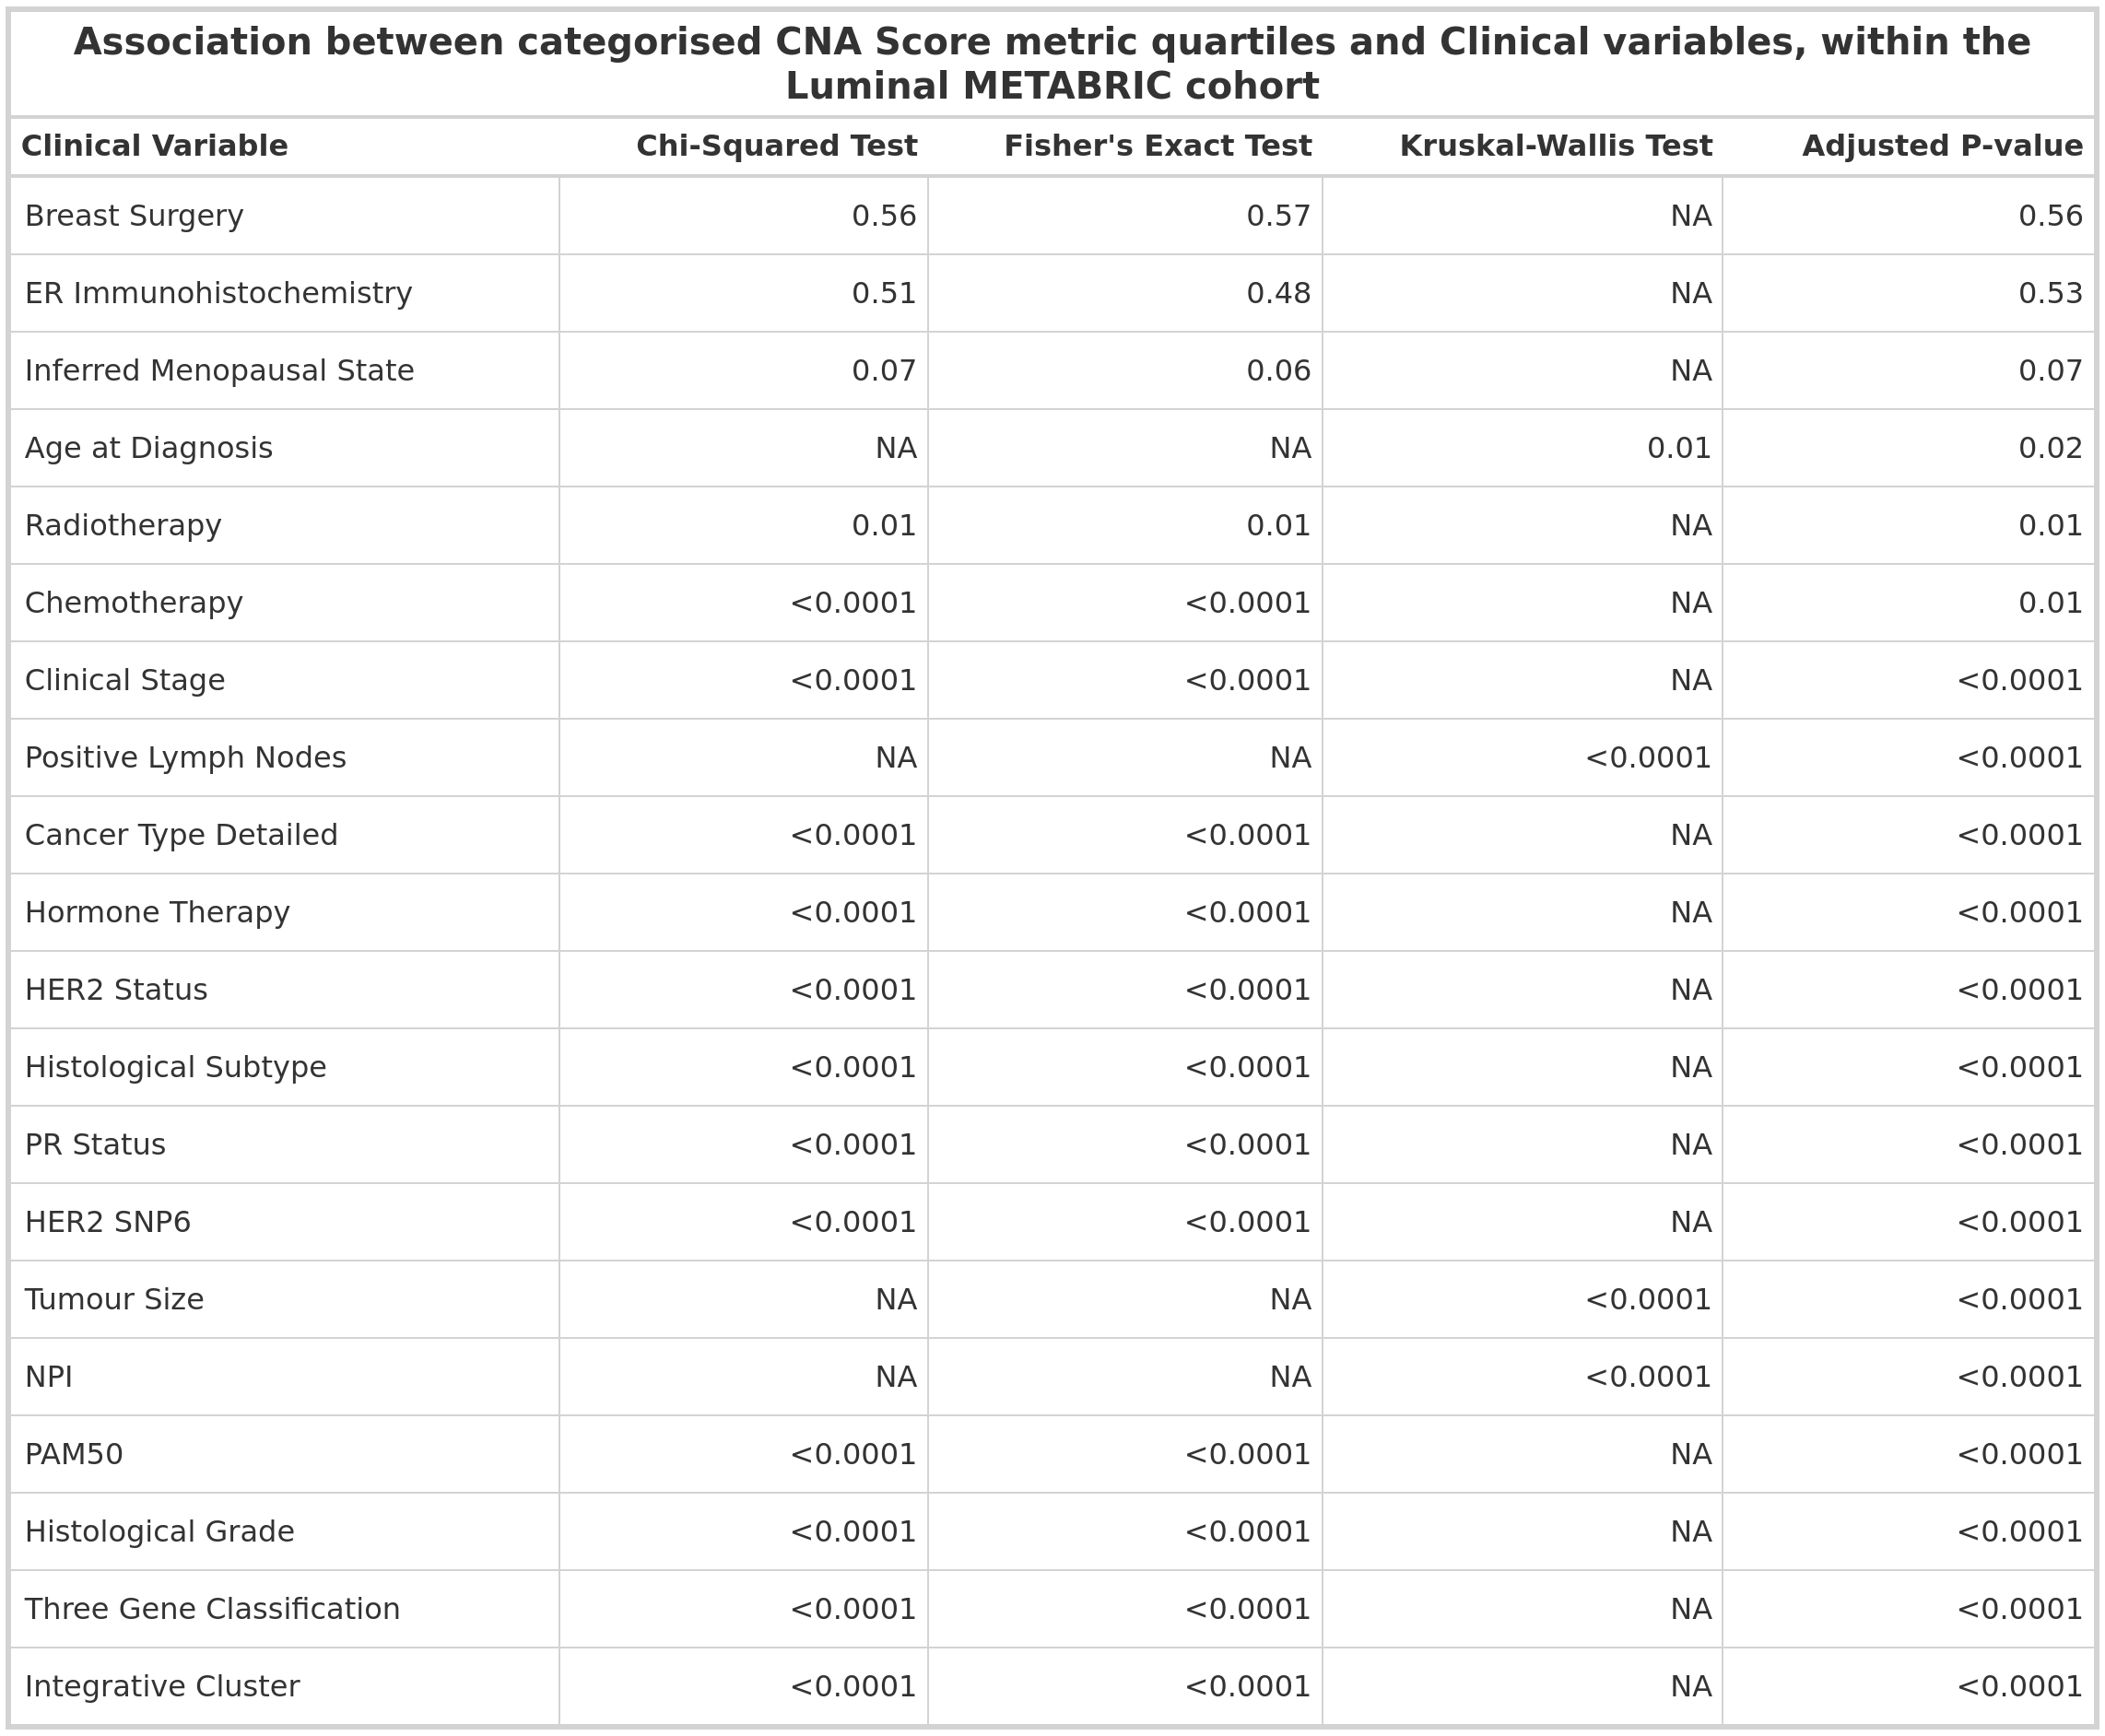
\includegraphics[width=0.98\textwidth]{../tables/Chapter_3/CNA_Quartile_Clin_Association.png}
\label{tab:Assoc_Tests_Q}
\end{table}

Plotting the adjusted survival curves for Luminal A and Luminal B patients within the different Absolute CNA Score Quartiles illustrates how these estimated effects differ between the two subtypes. Adjusted survival curves represent the estimated effect of Absolute CNA Score Quartiles by plotting the predicted survival curves for Luminal A and Luminal B patients for each Absolute CNA Score Quartile, having adjusted for the effects of the other covariates in the multivariable Cox model, where other covariates are fixed at the median/mode values of those variables (Figure \ref{fig:CNAQuartileSurvivalAdusted}). Here we see that DSS curves comparing Absolute CNA Score Quartiles within Luminal A show significant differences while the differences observed in DSS curves comparing Absolute CNA Score Quartiles within Luminal B are small and non-significant.  

\begin{table}[!htb]
\tiny
\caption[Final multivariable CPH model for disease-specific survival (Absolute CNA Score Quartiles).]{Final multivariable CPH model for disease-specific survival. Including selected clinical variables, Absolute CNA Score Quartiles and an interaction term, within the Luminal METABRIC cohort.}
\centering
\resizebox{\textwidth}{!}{ 
    \begin{tabular}{lccccl}
    \hline
    \textbf{Clinical Variable} & \textbf{Beta} & \textbf{SE} & \textbf{HR} & \textbf{95\% CI} & \textbf{P-value} \\ 
    \hline
    PAM50: &  &  &  &  & \\ 
    Luminal A (Ref) & - & - & - & - & - \\ 
    Luminal B & 1.069 & 0.299 & 2.912 & (1.619 - 5.237) & $<$0.001 \\
    Histological Grade: &  &  &  &  & \\
    1 (Ref) & - & - & - & - & -\\ 
    2 & 0.381 & 0.254 & 1.464 & (0.889 - 2.410) & 0.134 \\ 
    3 & 0.528 & 0.262 & 1.696 & (1.014 - 2.837) & 0.044 \\ 
    Tumour Size & 0.015 & 0.003 & 1.015 & (1.010 - 1.020) & $<$0.001 \\
    Positive Lymph Nodes & 0.050 & 0.008 & 1.051 & (1.034 - 1.069) & $<$0.001 \\ 
    Age at Diagnosis & 0.018 & 0.005 & 1.018 & (1.008 - 1.029) & $<$0.001 \\ 
    HER2 Status: &  &  &  &  & \\ 
    Negative (Ref) & - & - & - & - & - \\ 
    Positive & 0.541 & 0.202 & 1.717 & (1.157 - 2.550) & 0.007\\ 
    CNA Quartile: &  &  &  &  & \\ 
    CNA Q1 (Ref) & - & - & - & - & - \\ 
    CNA Q2 & 0.315 & 0.256 & 1.370 & (0.829 - 2.265) & 0.219 \\ 
    CNA Q3 & 0.767 & 0.247 & 2.152 & (1.326 - 3.493) & 0.002\\ 
    CNA Q4 & 0.839 & 0.272 & 2.315 & (1.360 - 3.942) & 0.002 \\ 
    CNA Q2:LumB  & -0.764 & 0.395 & 0.466 & (0.215 - 1.010) & 0.053  \\
    CNA Q3:LumB & -0.730 & 0.364 & 0.482 & (0.236 - 0.983) & 0.045 \\ 
    CNA Q4:LumB & -0.909 & 0.370 & 0.403 & (0.195 - 0.831) & 0.014 \\ \hline
    Likelihood Ratio Test p-value & & & & & \textless{2e-16} \\
    Wald Test p-value & & & & & \textless{2e-16}\\
    Score (log-rank) Test p-value  & & & & &\textless{2e-16} \\  \hline 
    \multicolumn{7}{l}{\begin{tabular}[c]{@{}l@{}} 
        SE: Standard Error; HR: Hazard Ratio; CI: Confidence Interval
        \label{table_mcm}
        \end{tabular}} \\ \hline
    \end{tabular}}
\end{table}

\begin{table}[!htb]
\tiny
\caption[Final multivariable CPH model for disease-specific survival (Absolute CNA Score).]{Final multivariable CPH model for disease-specific survival. Including selected clinical variables, Absolute CNA Score and an interaction term, within the Luminal METABRIC cohort.}
\centering
\resizebox{\textwidth}{!}{ 
    \begin{tabular}{lccccl}
    \hline
    \textbf{Clinical Variable} & \textbf{Beta} & \textbf{SE} & \textbf{HR} & \textbf{95\% CI} & \textbf{P-value} \\ 
    \hline
    PAM50: &  &  &  &  & \\ 
    Luminal A (Ref) & - & - & - & - & - \\ 
    Luminal B & 0.896 & 0.225 & 2.450 & (1.576 - 3.808) & $<$0.001 \\
    Histological Grade: &  &  &  &  & \\
    1 (Ref) & - & - & - & - & - \\ 
    2 & 0.431 & 0.253 & 1.539 & (0.937 - 2.525) & 0.088 \\ 
    3 & 0.636 & 0.260  & 1.888  & (1.135 - 3.141) & 0.014 \\ 
    Tumour Size & 0.013 & 0.002 & 1.013 & (1.009 - 1.018) & $<$0.001 \\
    Positive Lymph Nodes & 0.049 &  0.009 & 1.050 & (1.033 - 1.068) & $<$0.001 \\ 
    Age at Diagnosis & 0.016 & 0.005 & 1.016 & (1.006 - 1.027) & 0.002 \\ 
    HER2 Status: &  &  &  &  & \\ 
    Negative (Ref) & - & - & - & - & - \\ 
    Positive & 0.568 & 0.201 & 1.765 & (1.191 - 2.615) & 0.005\\ 
    CNA Score & 6.05e-05 & 1.83e-05 & 1.000  & (1.000 - 1.000) & $<$0.001  \\ 
    CNA Score:LumB & -6.77e-05 & 2.69e-05 & 0.999 & (0.999 - 1.000) & 0.012\\ \hline
    Likelihood Ratio Test p-value & & & & & \textless{2e-16}\\
    Wald Test p-value & & & & & \textless{2e-16}\\
    Score (log-rank) Test p-value  & & & & &\textless{2e-16}\\  \hline 
    \multicolumn{7}{l}{\begin{tabular}[c]{@{}l@{}}
        SE: Standard Error; HR: Hazard Ratio; CI: Confidence Interval
        \label{table_mcms}
        \end{tabular}} \\ \hline
    \vspace{0.2cm}
    \end{tabular}}
\end{table}

\begin{figure}[!htb]
\centering
\begin{subfigure}[b]{0.49\linewidth}       
\centering
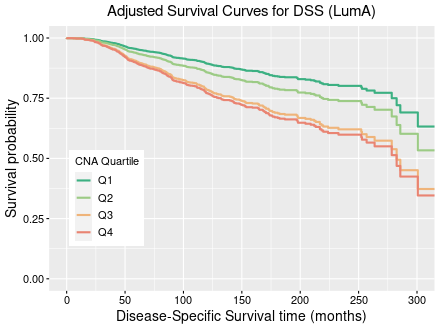
\includegraphics[width=\linewidth]{../figures/Chapter_3/LuminalA_Adsurvplot.png}
\caption{Luminal A Patients}
\label{fig:A}
\end{subfigure}
\begin{subfigure}[b]{0.49\linewidth}        
\centering
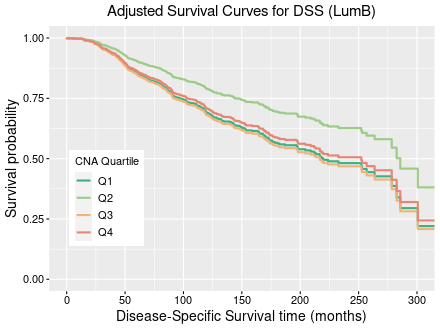
\includegraphics[width=\linewidth]{../figures/Chapter_3/LuminalB_Adsurvplot.png}
\caption{Luminal B Patients}
\label{fig:B}
\end{subfigure}
\caption[Adjusted survival curves for estimated Absolute CNA Score Quartile effects within each Luminal PAM50 subtype.]{Adjusted survival curves for estimated Absolute CNA Score Quartile effects within each Luminal PAM50 subtype. (A) Luminal A and (B) Luminal B breast cancer patients.}
\label{fig:CNAQuartileSurvivalAdusted}
\end{figure}
\FloatBarrier 

\subsubsection{Implementation of Recursive Partitioning Survival Trees}
Although the fitted models give strong indication that Absolute CNA Score, both as a continuous and categorical metric, can add value in modelling survival outcome in Luminal breast cancer, diagnostic tests indicate that the proportional hazards assumption may not be met (online Supplementary Information). As an alternative approach, recursive partitioning survival trees are fitted using the rpart and ctree algorithms. Recursive partitioning trees can explore the association between Absolute CNA Score and survival and examine any interactions between the six clinical variables that were significant in models including Absolute CNA Score variables. The predetermined Absolute CNA Score Quartiles can be fitted in the model as a predictor, but recursive partitioning trees also offer the added benefit of determining the optimum cut-off in Absolute CNA Score, implicit in the partitioning algorithm. 

Survival trees considering Absolute CNA Score Quartiles, with additional applications provided in Appendix A, suggest a similar partitioning with Absolute CNA Score Q1 and Q2 versus Absolute CNA Score Q3 and Q4, consistent with the effects estimated by the CPH model (Figure \ref{fig:LumAB_Trees_Quart}). Figure \ref{fig:LumAB_Trees_Quart} shows the survival tree fitted using the ctree algorithm, which indicates that for Luminal A patients who have 0-1 positive lymph nodes, tumour size less than 31mm and age of diagnosis less than 71.4 years, DSS outcome can be stratified by Absolute CNA Score Quartile, where patients with high GI show reduced survival probability than those with a lower GI ($p = 0.032$).   

Survival trees considering Absolute CNA Score, with additional applications provided in Appendix A, also suggest a similar partitioning consistent with the effects estimated by the CPH model and the survival trees considering Absolute CNA Score Quartiles (Figure \ref{fig:LumAB_Trees_Score}). In Figure \ref{fig:LumAB_Trees_Score}, the survival tree fitted using the ctree algorithm, Luminal A patients who have 0-1 positive lymph nodes, tumour size less than 31mm and age of diagnosis less than 71.4 years, DSS outcome can be stratified by Absolute CNA Score with optimised Absolute CNA Score cut-off point value 5,882 ($p = 0.005$). Including the continuous Absolute CNA Score, rather than the categorised Absolute CNA Score Quartile, allows a more nuanced investigation of the optimal Absolute CNA Score cut-off point. While the estimated optimal cut-off of 5,882 is close to 5,547, the boundary between Absolute CNA Score Quartile 2 and 3, utilising the Absolute CNA Score cut-off results in 20 patients being reclassified to the low-risk group.  

Overall, the survival trees indicate that the Absolute CNA Score metric, implemented either as predetermined categorised quartiles or original continuous variable, can stratify subsets of patients based on DSS and therefore help identify Luminal A patients who are at elevated risk.  

\begin{figure}[!htb]
\centering
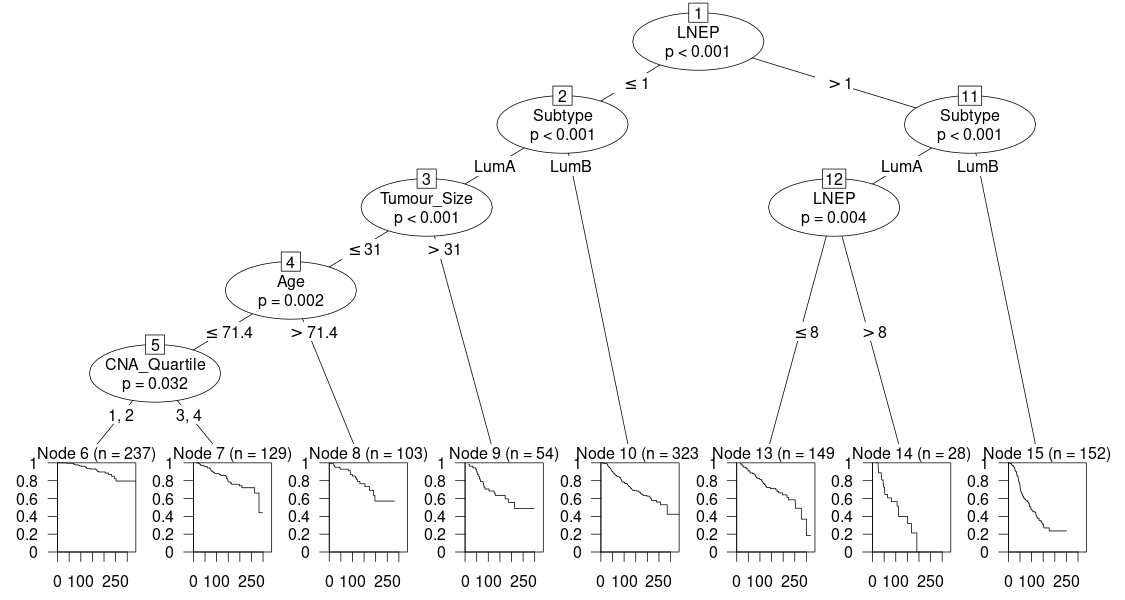
\includegraphics[width=\linewidth]{../figures/Chapter_3/LuminalAB_Ctree_DSS_Quart.png}
\caption[Recursive partitioning survival tree for disease-specific survival using clinical variables and Absolute CNA Score Quartile as candidate predictors (ctree).]{Recursive partitioning survival tree for disease-specific survival using clinical variables and Absolute CNA Score Quartile as candidate predictors. Fitted using the ctree algorithm.}
\label{fig:LumAB_Trees_Quart}
\end{figure}

\begin{figure}[!htb]
\centering
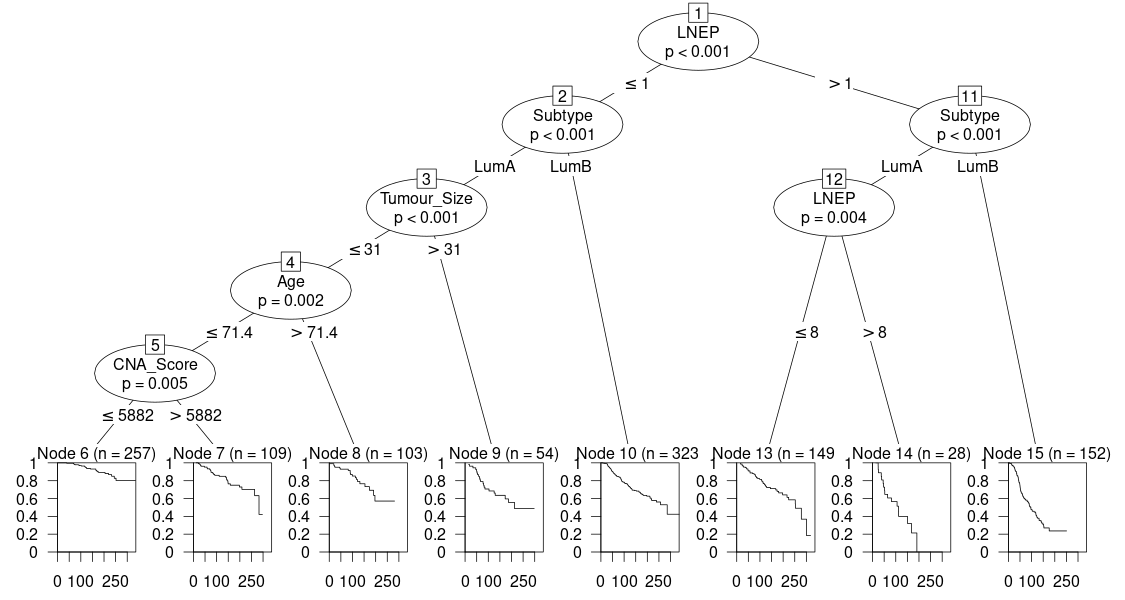
\includegraphics[width=\linewidth]{../figures/Chapter_3/LuminalAB_Ctree_DSS_Score.png}
\caption[Recursive partitioning survival tree for disease-specific survival using clinical variables and Absolute CNA Score as candidate predictors (ctree).]{Recursive partitioning survival tree for disease-specific survival using clinical variables and Absolute CNA Score as candidate predictors. Fitted using the ctree algorithm.}
\label{fig:LumAB_Trees_Score}
\end{figure}
\clearpage

\subsection{Analysis of Global CNA Metrics across All METABRIC Patients}
Expanding the study focus to all patients, i.e. all PAM50 subtypes (Basal, HER2, Luminal B, Luminal A, Normal and Claudin-low), associations between the six global CNA Score metrics and six global CNA Burden metrics with survival are examined in this section. The global CNA metrics are initially included with PAM50 subtype or IntClust molecular classifications to assess whether the CNA metric information can add additional prognostic value to the molecular classifications, and then included with a selection of clinical variables to explore interactions between the clinical variables and CNA metrics. Given the large number of candidate predictors under consideration, the fact that the CPH assumption may not be met, and the benefit of the partitioning trees in determining optimal cut-off, recursive partitioning survival trees are implemented. 

\subsubsection{CNA Metric Survival Trees, in Combination with Molecular Classification Predictors} 
A range of survival trees for OS, DSS, 5-year OS and DSS, and 10-year OS and DSS are produced. These trees include the six global CNA Score metrics: Absolute CNA Score, CNA Amp Score, CNA Del Score, Difference Score, Percentage Amp Score and Percentage Del Score, or the six global CNA Burden metrics: CNA Burden, CNA Amp Burden, CNA Del Burden, Difference Burden, Percentage Amp Burden and Percentage Del Burden, with PAM50 subtype or IntClust molecular classifications. Depending on the algorithm used (rpart or ctree) a number of different global CNA Score and Burden metrics are selected as useful predictors when modelling survival outcomes. The survival trees for DSS outcomes are displayed and discussed below, while the survival trees for OS outcomes are provided in Appendix B. 

Initially survival trees including only PAM50 subtype (Figure \ref{fig:PAM50_Indv_Surv_Trees}) or IntClust (Figure \ref{fig:IC_Indv_Surv_Trees}) as candidate predictors are fitted, indicating which subtypes display similarity in survival outcome and providing information on partitions in trees where only molecular classification is included.

\captionsetup[subfigure]{font={normalfont, small}, skip=1pt, margin=-0.0cm, singlelinecheck=false}

\begin{figure}[!h]
\begin{minipage}{.44\textwidth}
\begin{subfigure}{\textwidth}
\subcaption{}
\includegraphics[width=\linewidth, height = 5.7cm]{../figures/Chapter_3/Ind_Partykit_Survival_Score_DSS_PAM50.png}
\end{subfigure}\par
\end{minipage}
\begin{minipage}{.55\textwidth}
\begin{subfigure}{\textwidth}
\subcaption{}
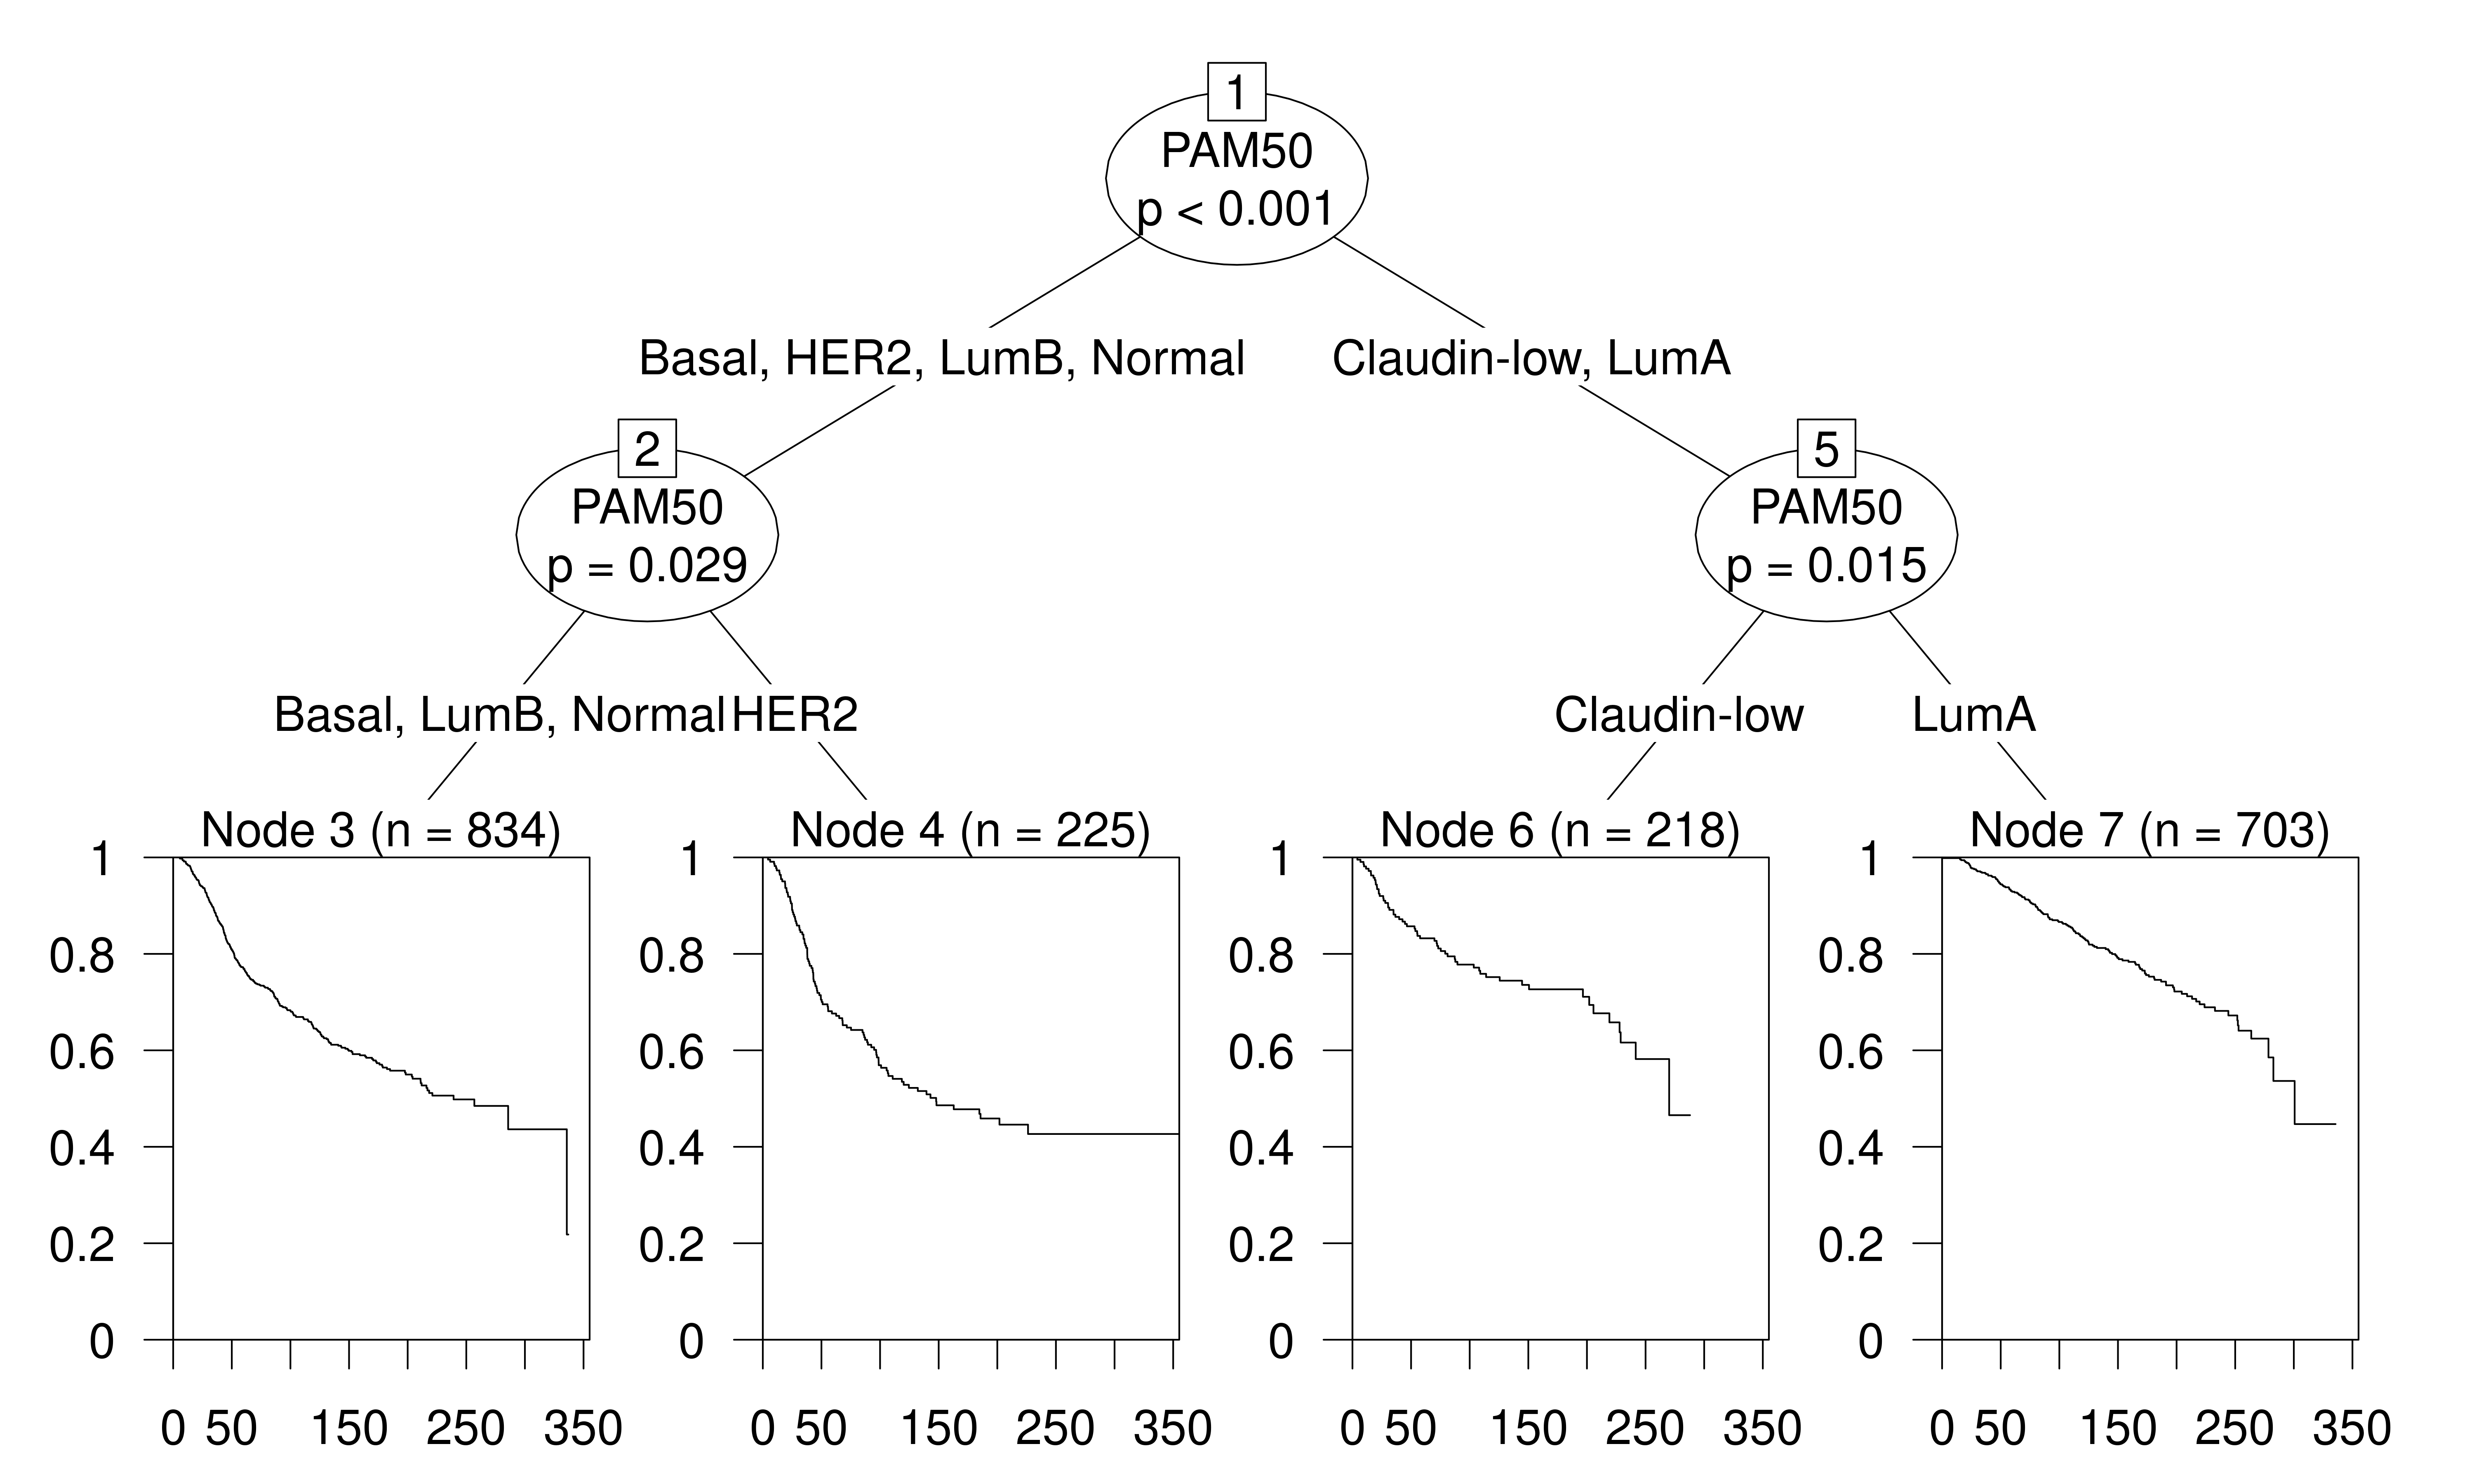
\includegraphics[width=\linewidth, height = 5.7cm]{../figures/Chapter_3/Ind_Ctree_Survival_Score_DSS_PAM50.png}
\end{subfigure}\par
\end{minipage}

\caption[Recursive partitioning survival trees for disease-specific survival using PAM50 subtype as a candidate predictor.]{Recursive partitioning survival trees for disease-specific survival using PAM50 subtype as a candidate predictor. (A) Trees fitted using the rpart algorithm and (B) trees fitted using the ctree algorithm.}
\label{fig:PAM50_Indv_Surv_Trees}
\end{figure}

\begin{figure}[!h]
\begin{minipage}{.44\textwidth}
\begin{subfigure}{\textwidth}
\subcaption{}
\includegraphics[width=\linewidth, height = 5.7cm]{../figures/Chapter_3/Ind_Partykit_Survival_Score_DSS_INTCLUST.png}
\end{subfigure}\par
\end{minipage}
\begin{minipage}{.55\textwidth}
\begin{subfigure}{\textwidth}
\subcaption{}
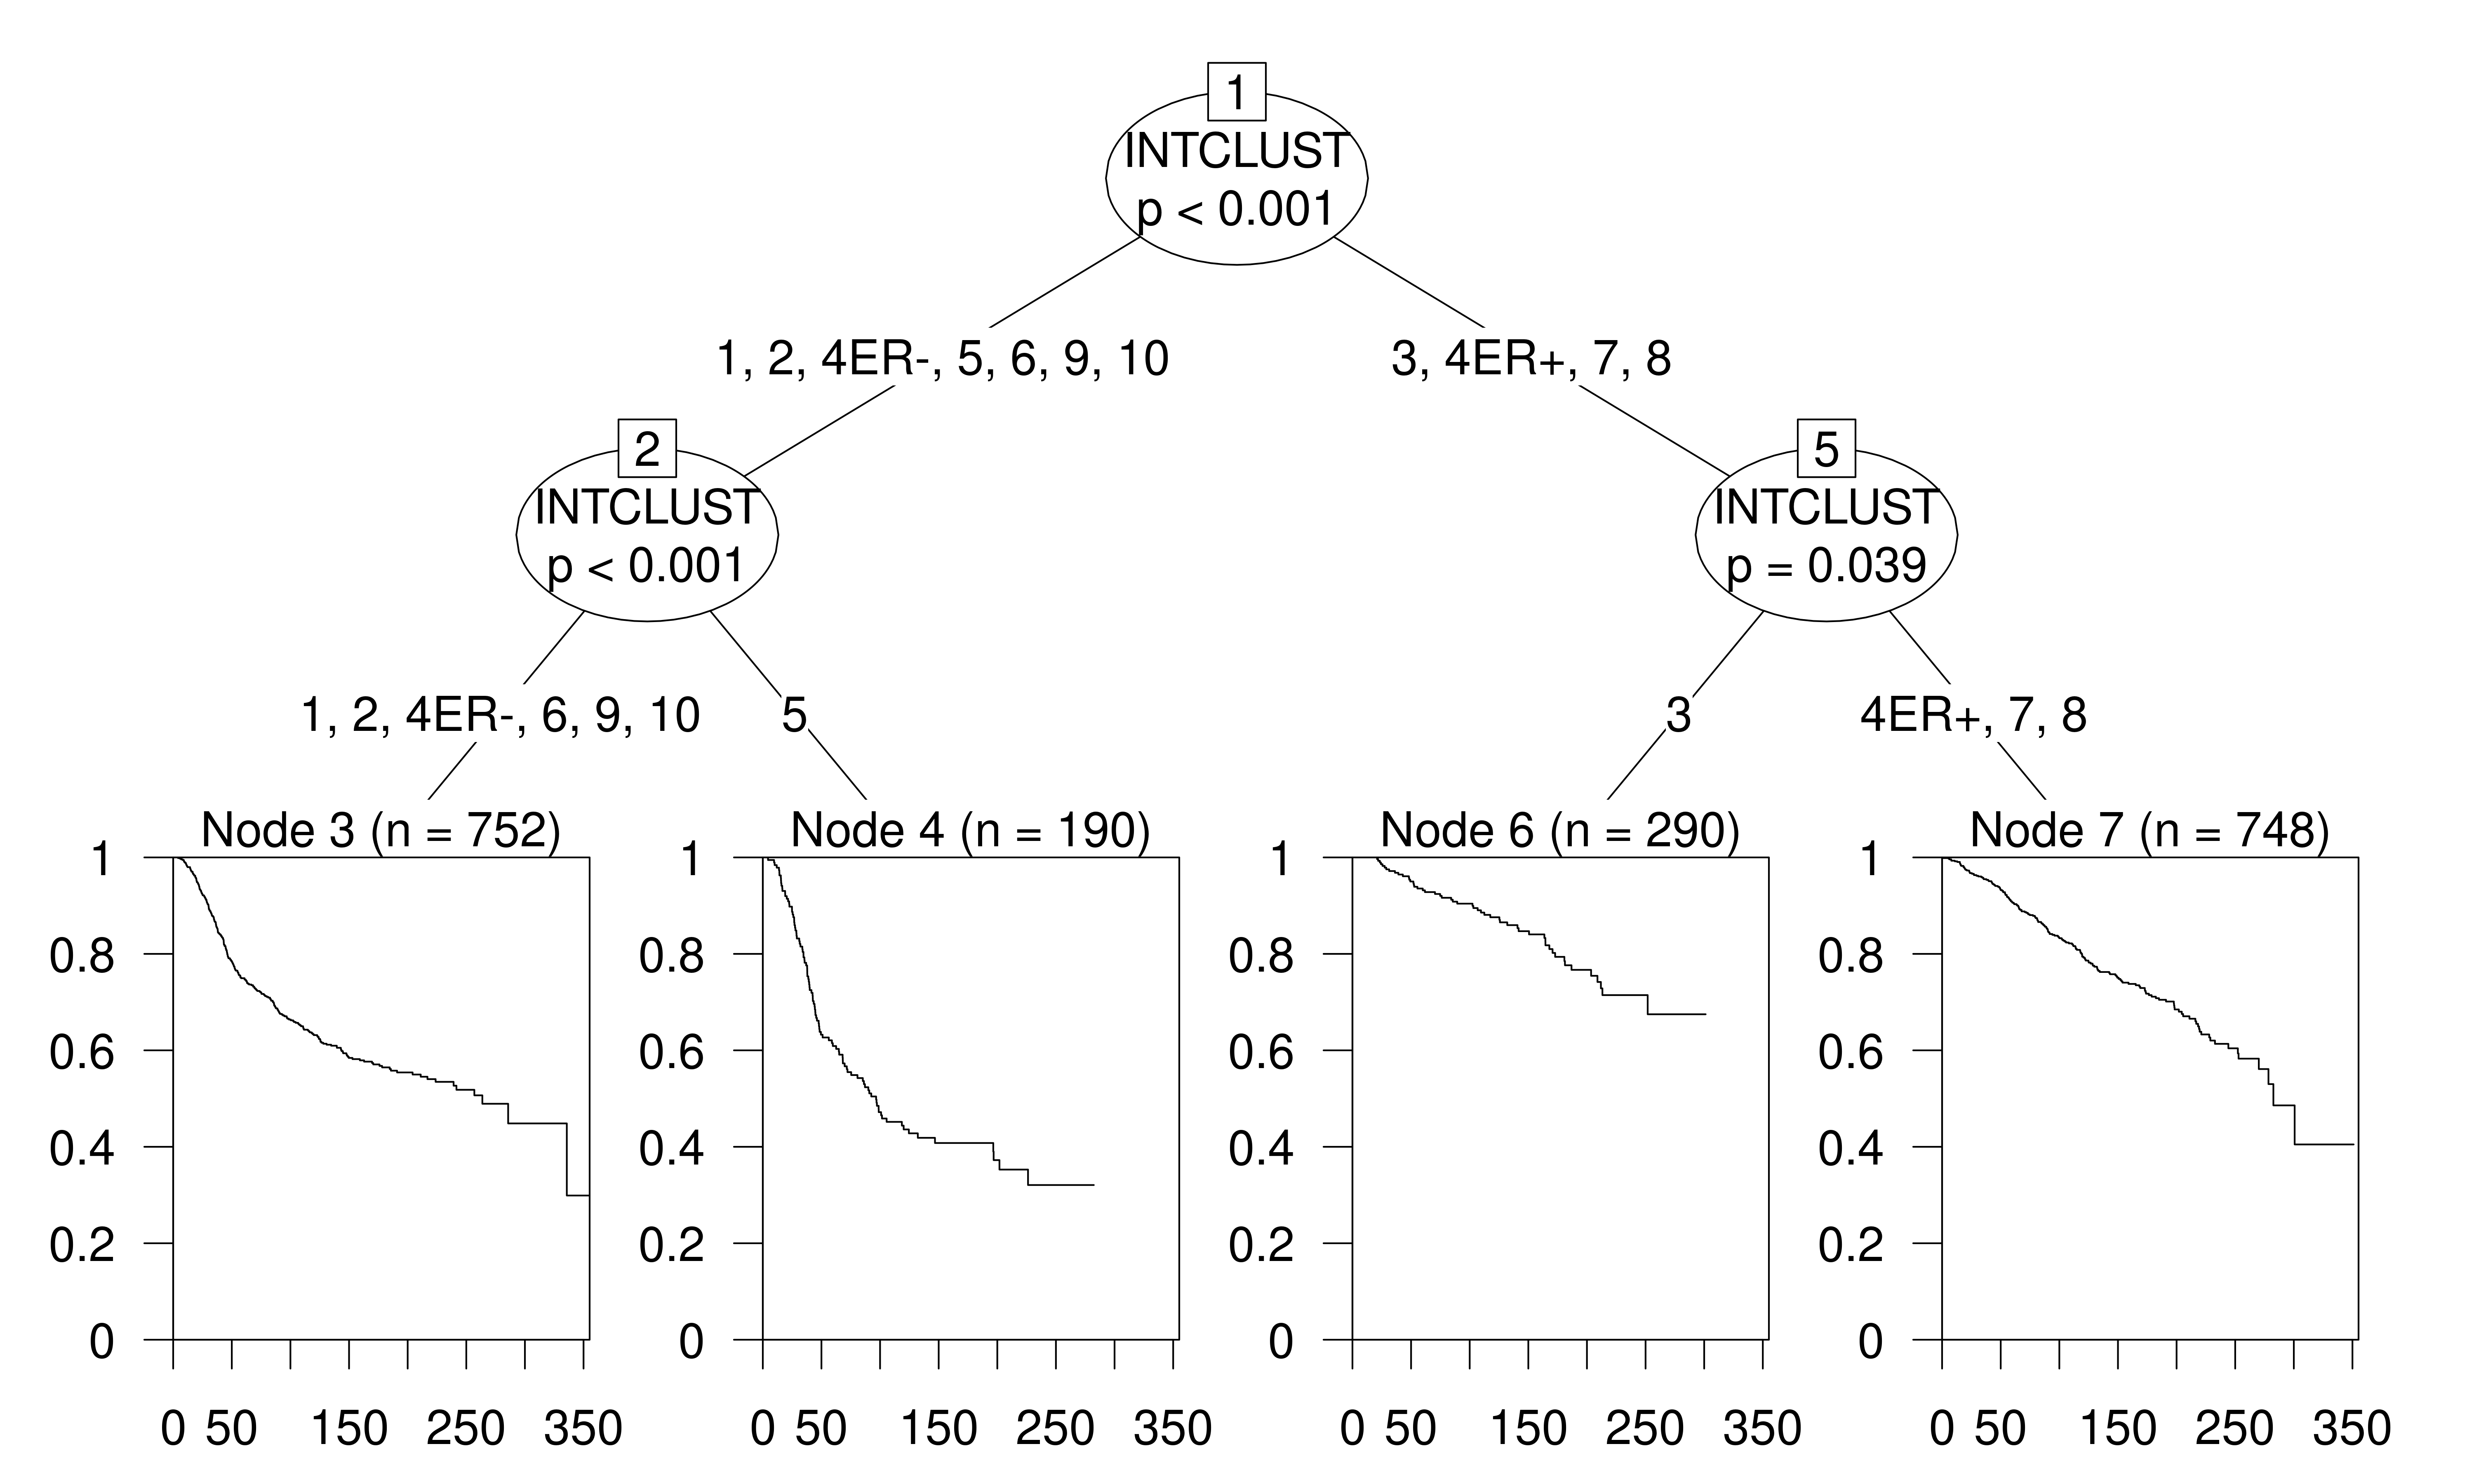
\includegraphics[width=\linewidth, height = 5.7cm]{../figures/Chapter_3/Ind_Ctree_Survival_Score_DSS_INTCLUST.png}
\end{subfigure}\par
\end{minipage}

\caption[Recursive partitioning survival trees for disease-specific survival using Integrative Cluster as a candidate predictor.]{Recursive partitioning survival trees for disease-specific survival using Integrative Cluster as a candidate predictor. (A) Trees fitted using the rpart algorithm and (B) trees fitted using the ctree algorithm.}
\label{fig:IC_Indv_Surv_Trees}
\end{figure}

Focusing on survival trees for DSS, 5-year DSS and 10-year DSS, that have the six CNA Score metrics and PAM50 molecular classification as candidate predictors, indicates CNA Del Score to be a consistently significant factor (Figure \ref{fig:PAM50_CNA_Score_DSS}, \ref{fig:PAM50_CNA_Score_FiveYearDSS} and \ref{fig:PAM50_CNA_Score_TenYearDSS}). While variation in the predictors used to partition the data is observed across survival outcome (DSS, 5-year DSS or 10-year DSS) and algorithm (rpart or ctree), CNA Del Score appears to add additional prognostic value to the PAM50 subtypes, primarily Luminal A and Claudin-low subtypes. Patients within these subtypes, displaying higher levels of CNA Del Score, have poorer outcome with respect to DSS, 5-year and 10-year DSS. Consistency is observed in the CNA Del Score cut-off points chosen by the ctree algorithm across the three survival outcomes. The optimal cut-off point for CNA Del Score for trees produced using the ctree algorithm is 3,286 in Luminal A and Claudin-low patients (Figure \ref{fig:PAM50_CNA_Score_DSS}B), 3,286 in Luminal A patients (Figure \ref{fig:PAM50_CNA_Score_FiveYearDSS}B), and 3,138 in Luminal A, Claudin-low and Normal patients (Figure \ref{fig:PAM50_CNA_Score_TenYearDSS}B), for DSS, 5-year DSS and 10-year DSS. 

When considering the survival trees for DSS, 5-year DSS and 10-year DSS, generated using the six CNA Burden metrics and PAM50 molecular classification as candidate predictors, similar tree structures are observed (Figures \ref{fig:PAM50_CNA_Burden_DSS}, \ref{fig:PAM50_CNA_Burden_FiveYearDSS}, and \ref{fig:PAM50_CNA_Burden_TenYearDSS}). CNA Del Burden is again consistently selected as an important predictor in the context of DSS, partitioning Luminal A and Claudin-low subtypes using a cut-off of 18.28\% (Figure \ref{fig:PAM50_CNA_Burden_DSS}B), 5-year DSS, partitioning Luminal A subtype using a cutoff of 14.55\% (Figure \ref{fig:PAM50_CNA_Burden_FiveYearDSS}B), and 10-year DSS, partitioning Luminal A, Claudin-low and Normal subtypes using a cutoff of 14.02\% (Figure \ref{fig:PAM50_CNA_Burden_TenYearDSS}B). 

In the survival trees for DSS, 5-year DSS and 10-year DSS, generated using the six CNA Score metrics and IntClust molecular classification as candidate predictors, CNA Del Score consistently appears as an important predictor for survival outcome, in patients corresponding to IntClust 3, 4ER+, 7 and 8 (Figures \ref{fig:INTCLUST_CNA_Score_DSS}-\ref{fig:INTCLUST_CNA_Score_TenYearDSS}). Again, the optimal cut-off points are fairly consistent, in all but one tree, at values 1,469.5 and 1,469 for DSS (Figure \ref{fig:INTCLUST_CNA_Score_DSS}), 1,933 and 3,722 for 5-year DSS (Figure \ref{fig:INTCLUST_CNA_Score_FiveYearDSS}), and 1,469.5 and 1,989 for 10-year DSS (Figure \ref{fig:INTCLUST_CNA_Score_TenYearDSS}). Patients within IntClust 3, 4ER+, 7 and 8, displaying levels of CNA Del Score above the optimal cut-off point have worse DSS, 5 and 10-year DSS, than patients displaying levels of CNA Del Score below the optimal cut-off point. 

Considering survival trees for DSS, 5-year DSS and 10-year DSS, with the six CNA Burden metrics and IntClust molecular classification as candidate predictors, indicate similar tree structures (Figures \ref{fig:INTCLUST_CNA_Burden_DSS}-\ref{fig:INTCLUST_CNA_Burden_TenYearDSS}). Again, all trees initially split on IntClust, with CNA Del Burden consistently selected as an additional significant predictor in the context of the DSS, 5-year DSS and 10-year DSS. 

It appears that the CNA Del Score and Burden metrics are associated with DSS, 5-year DSS and 10-year DSS. The majority of the survival trees showed that the CNA Del metrics are useful in splitting Luminal A and Claudin-low patients, and IntClust 3, 4ER+, 7 and 8 patients, into groups with distinct survival outcomes. Interestingly, a known feature of these PAM50 subtypes and IntClusts is that they display low genomic instability and good prognosis \citep{pmid22522925}, Section \ref{LGI}. This may explain why the optimal cut-off points for the CNA Del Score and Burden are quite low. In Chapter 2, we observed that PAM50 subtypes associated with poorer survival (Basal, HER2 and Luminal B) have significantly higher levels of deletions. Here, we observe that within PAM50/IntClust classifications associated with good prognosis, that have CNA Del Score and Burden over an optimised threshold, patients having poorer survival outcomes, again indicating that high levels of deletions are more detrimental than other forms of alterations.

\begin{figure}[!h]
\centering

\vspace{0.5cm}

\begin{subfigure}{\textwidth}
\subcaption{}
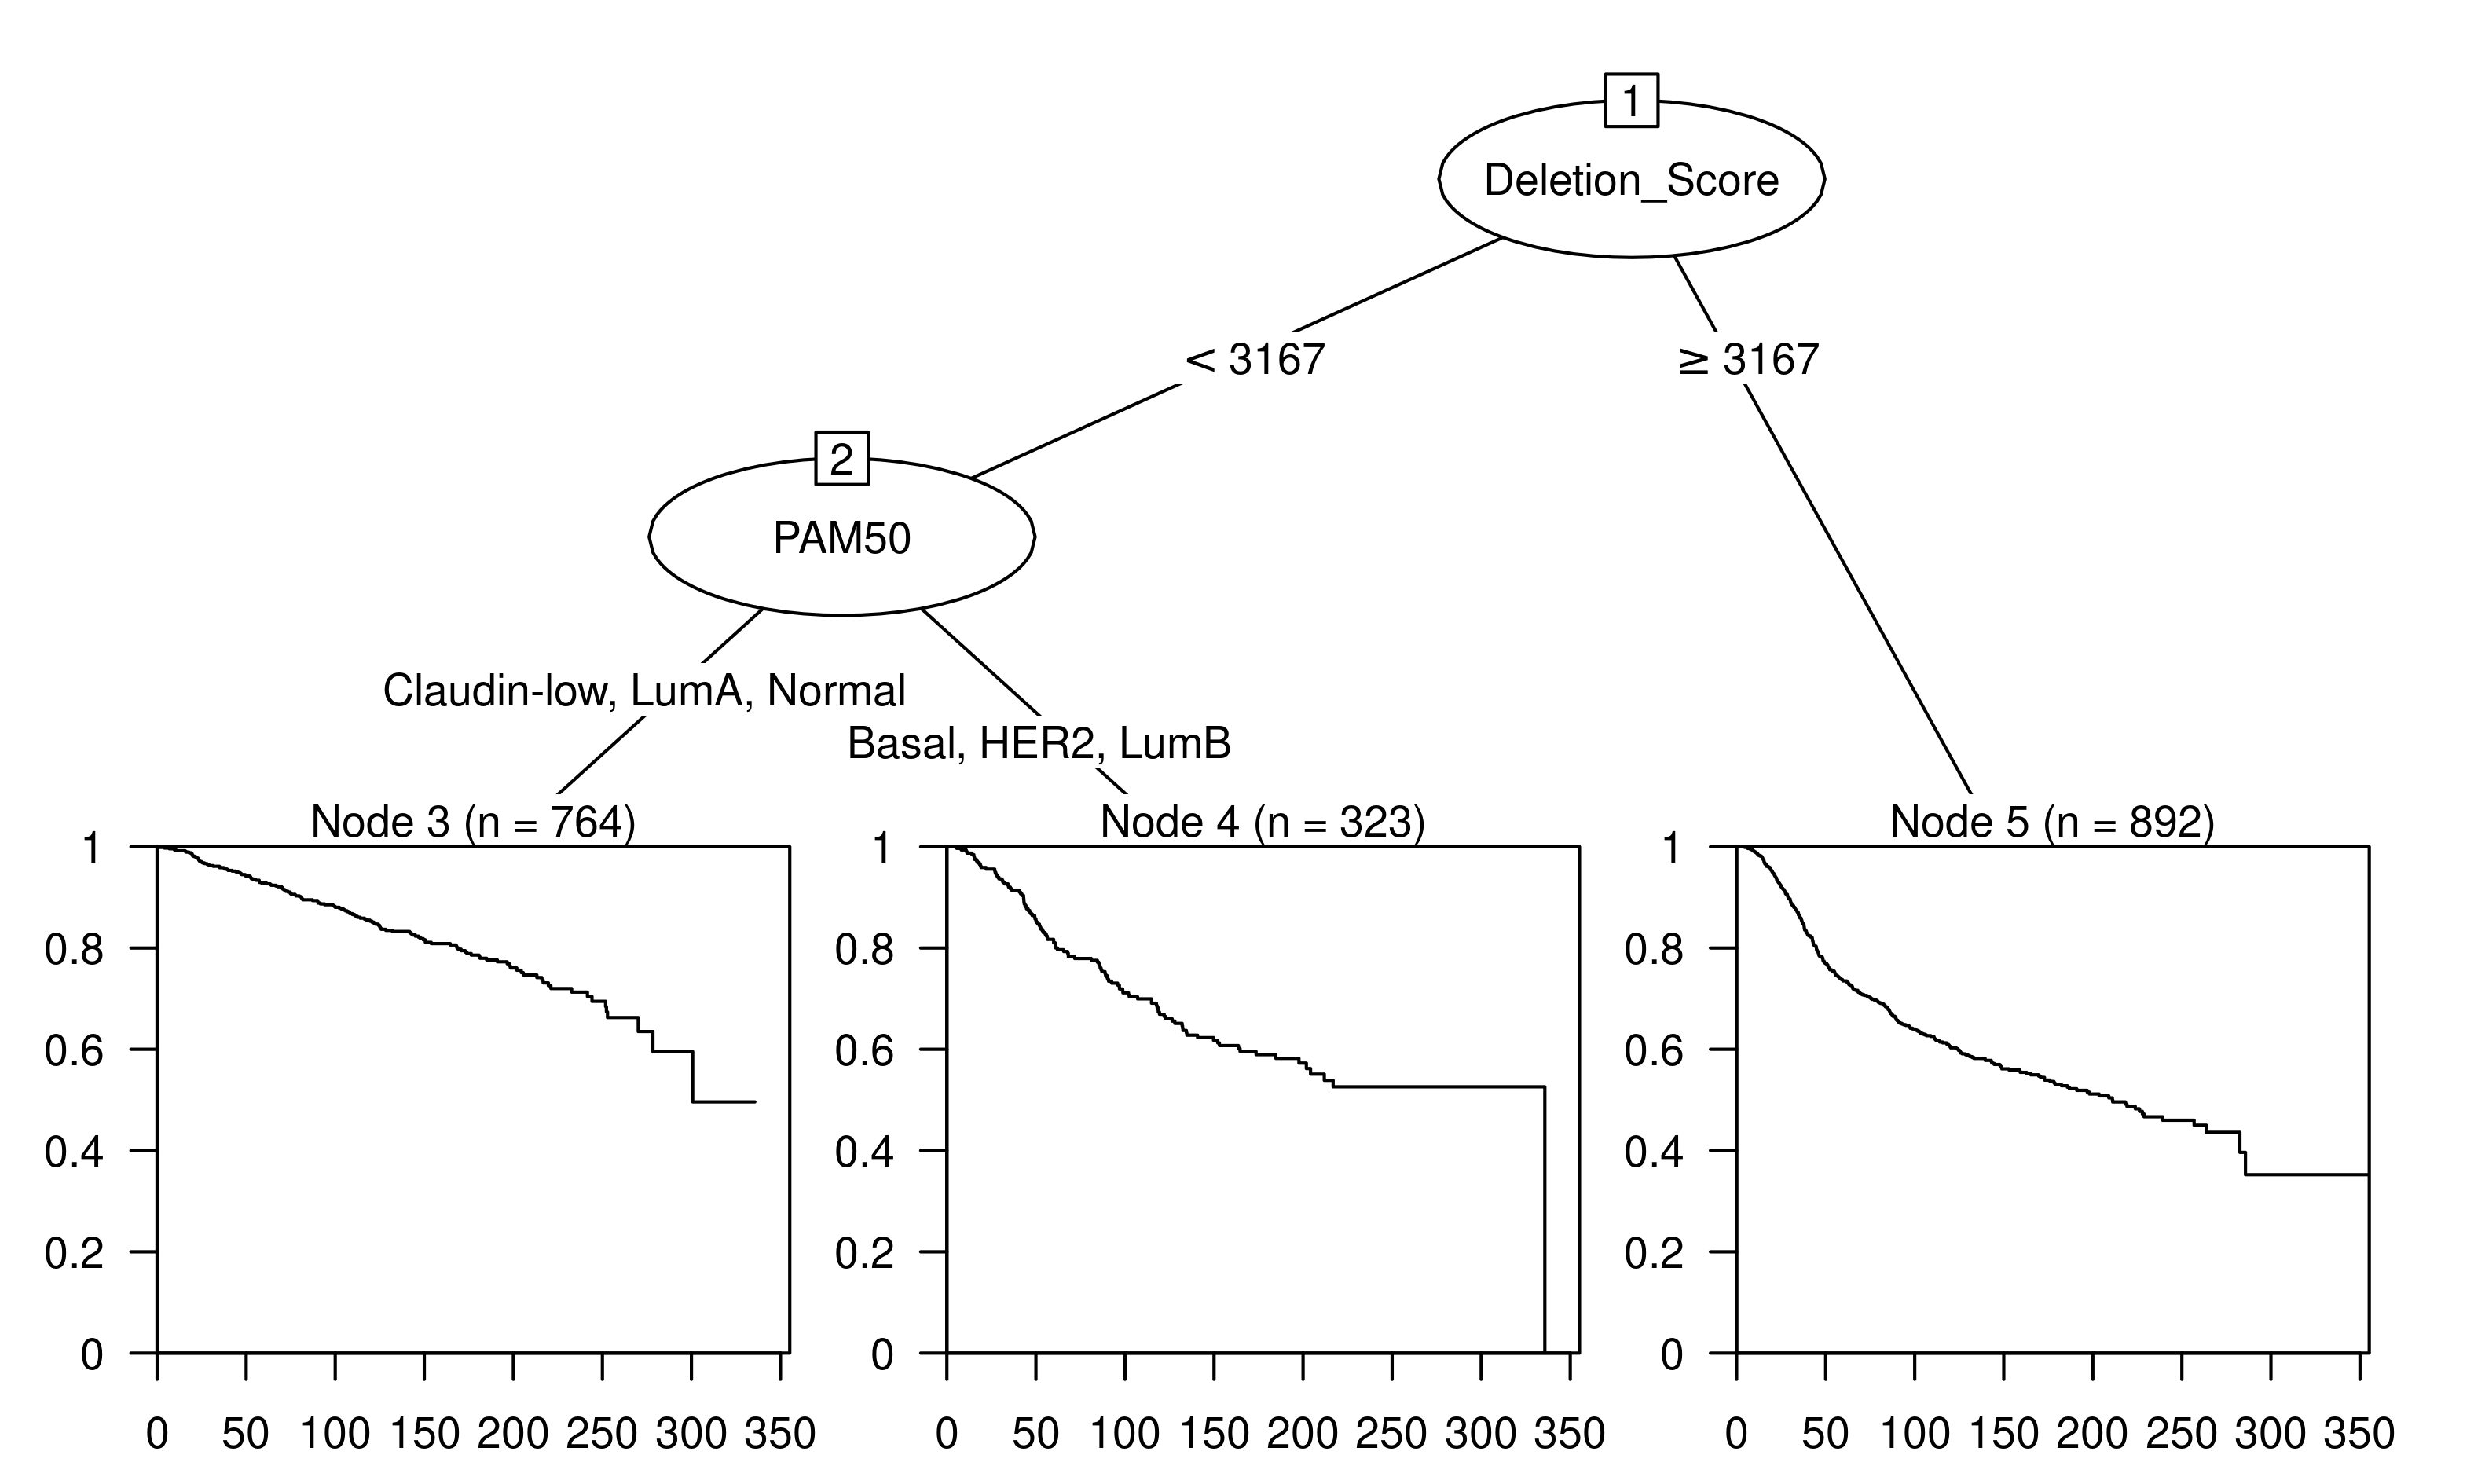
\includegraphics[width=1\textwidth]{../figures/Chapter_3/PartyKit_Survival_Score_DSS_PAM50.png}
\end{subfigure}

\vspace{2cm}

\begin{subfigure}{\textwidth}
\subcaption{}
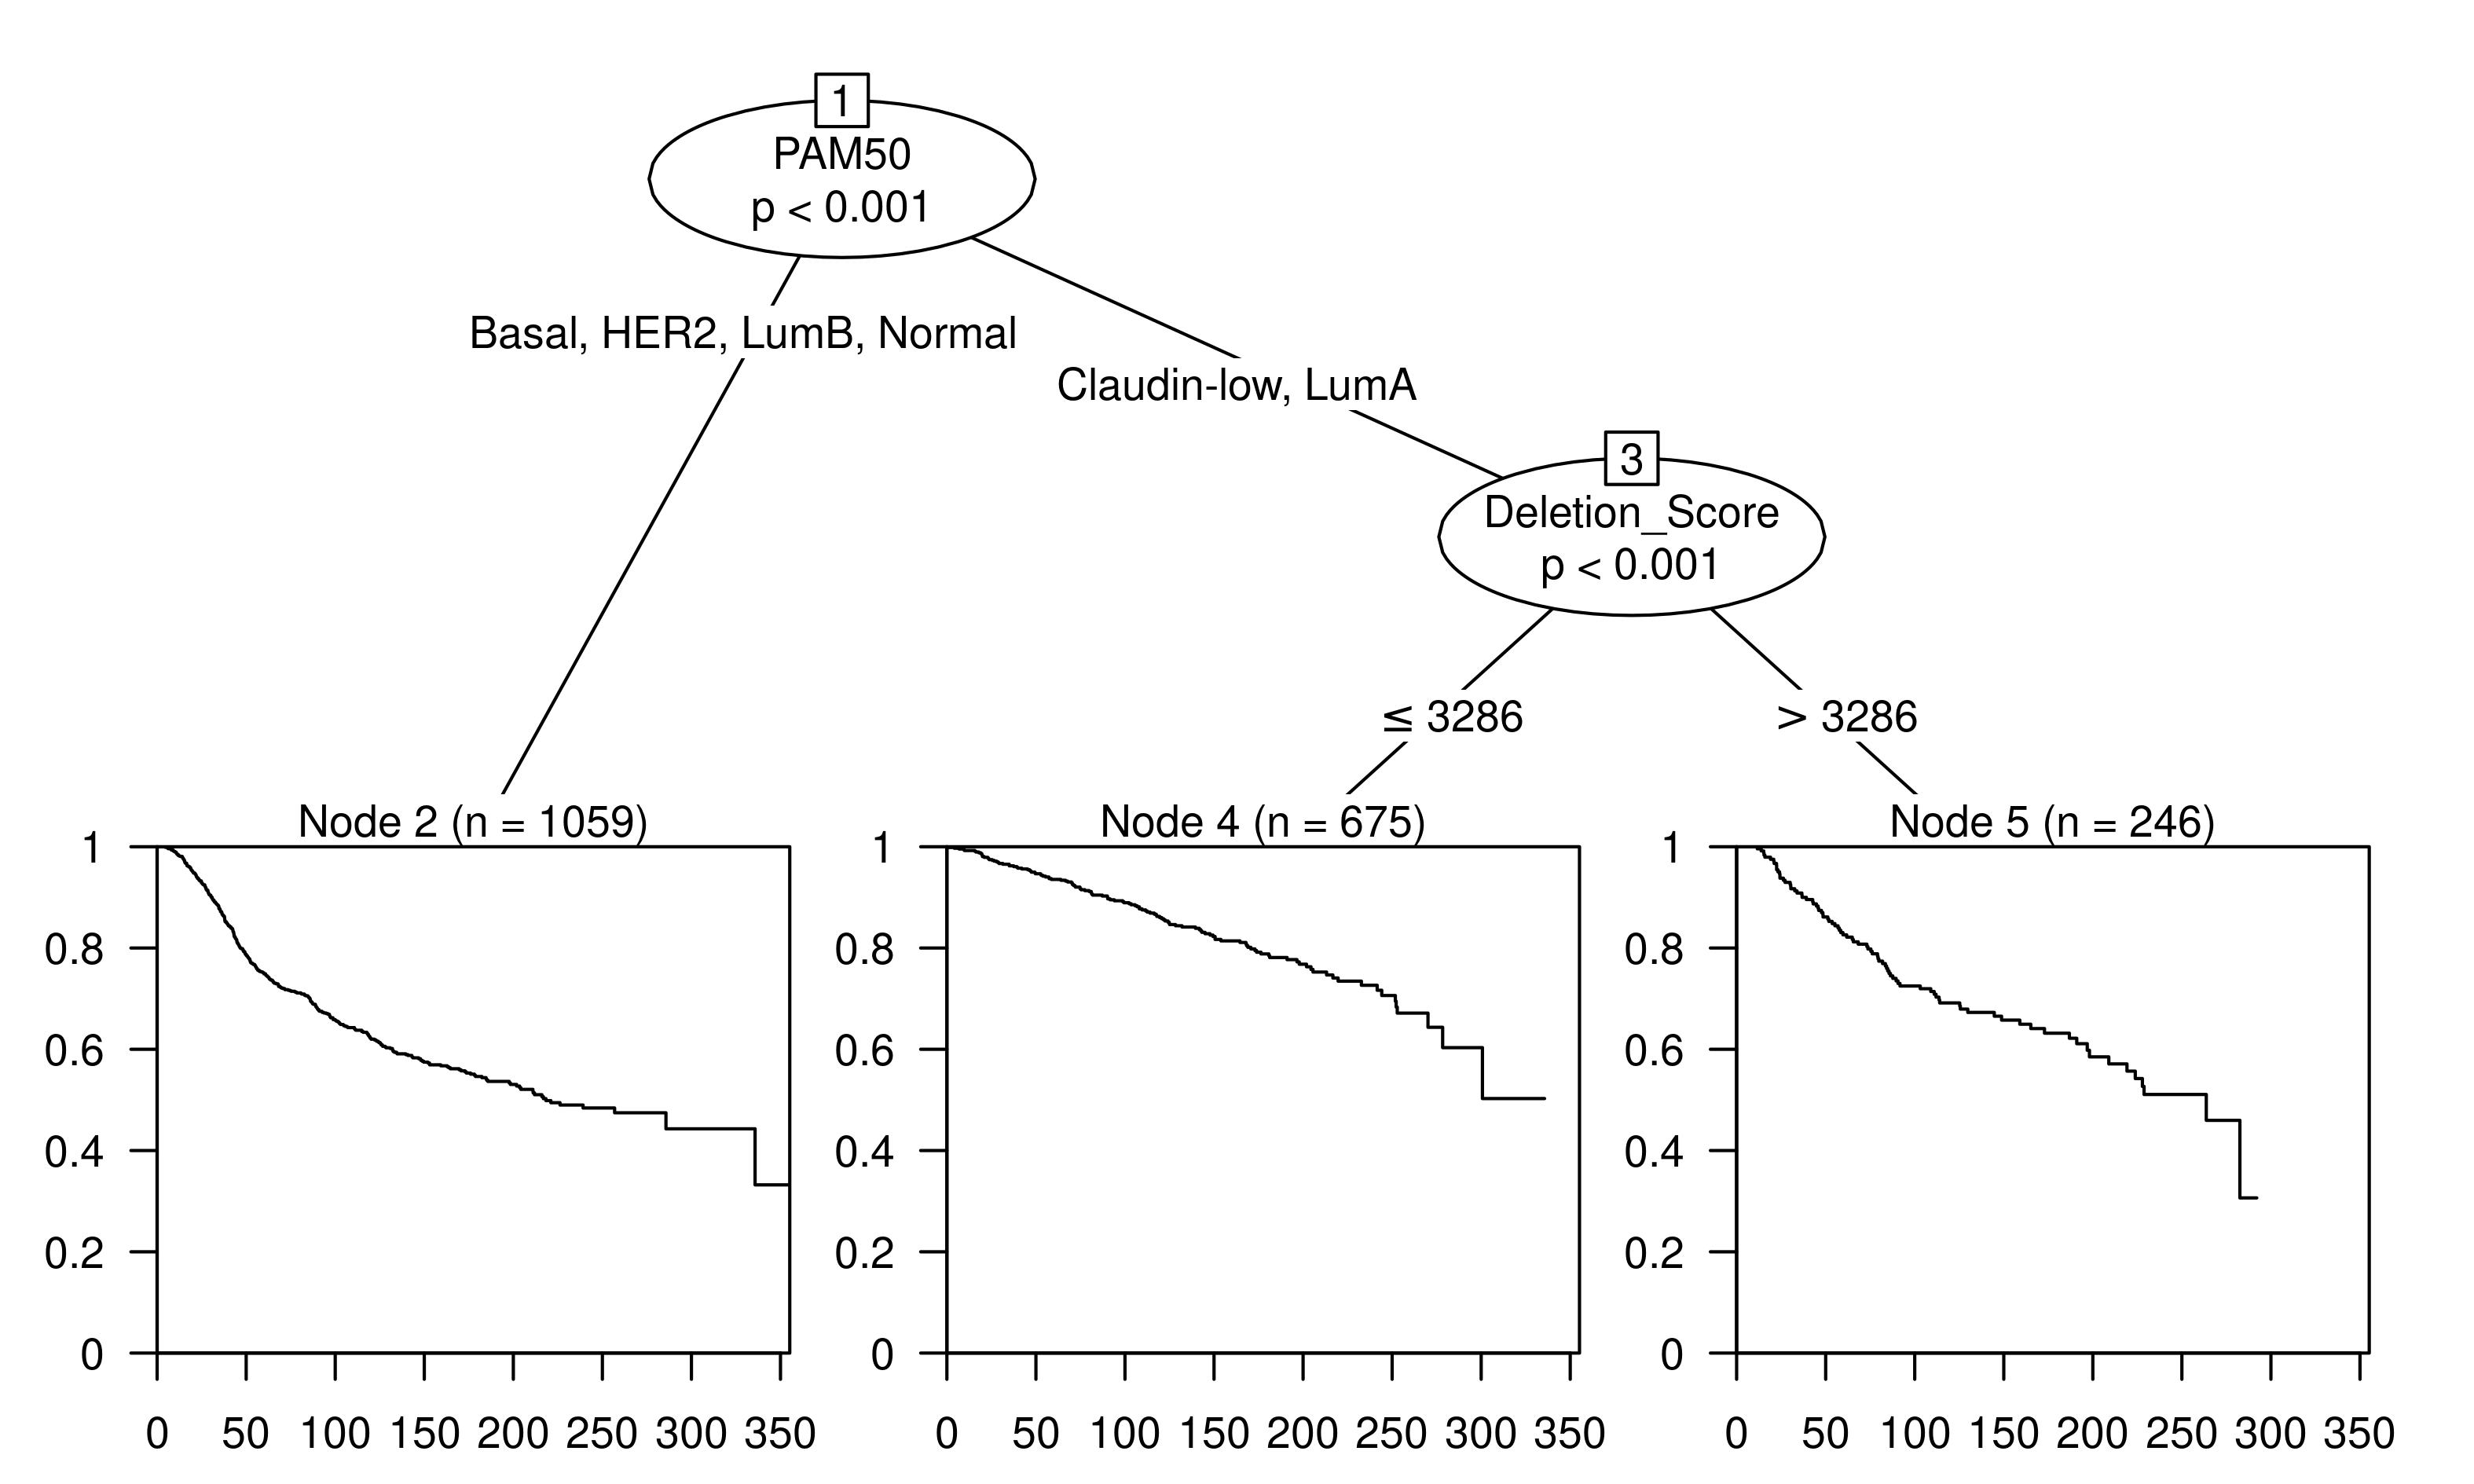
\includegraphics[width=1\textwidth]{../figures/Chapter_3/Ctree_Survival_Score_DSS_PAM50.png}
\end{subfigure}

\vspace{0.5cm}

\caption[Recursive partitioning survival trees for disease-specific survival using PAM50 subtype and the six CNA Score metrics as candidate predictors.]{Recursive partitioning survival trees for disease-specific survival using PAM50 subtype and the six CNA Score metrics as candidate predictors. (A) Trees fitted using the rpart algorithm and (B) trees fitted using the ctree algorithm.}
\label{fig:PAM50_CNA_Score_DSS}
\end{figure}

\begin{figure}[!h]
\centering

\vspace{0.5cm}

\begin{subfigure}{\textwidth}
\subcaption{}
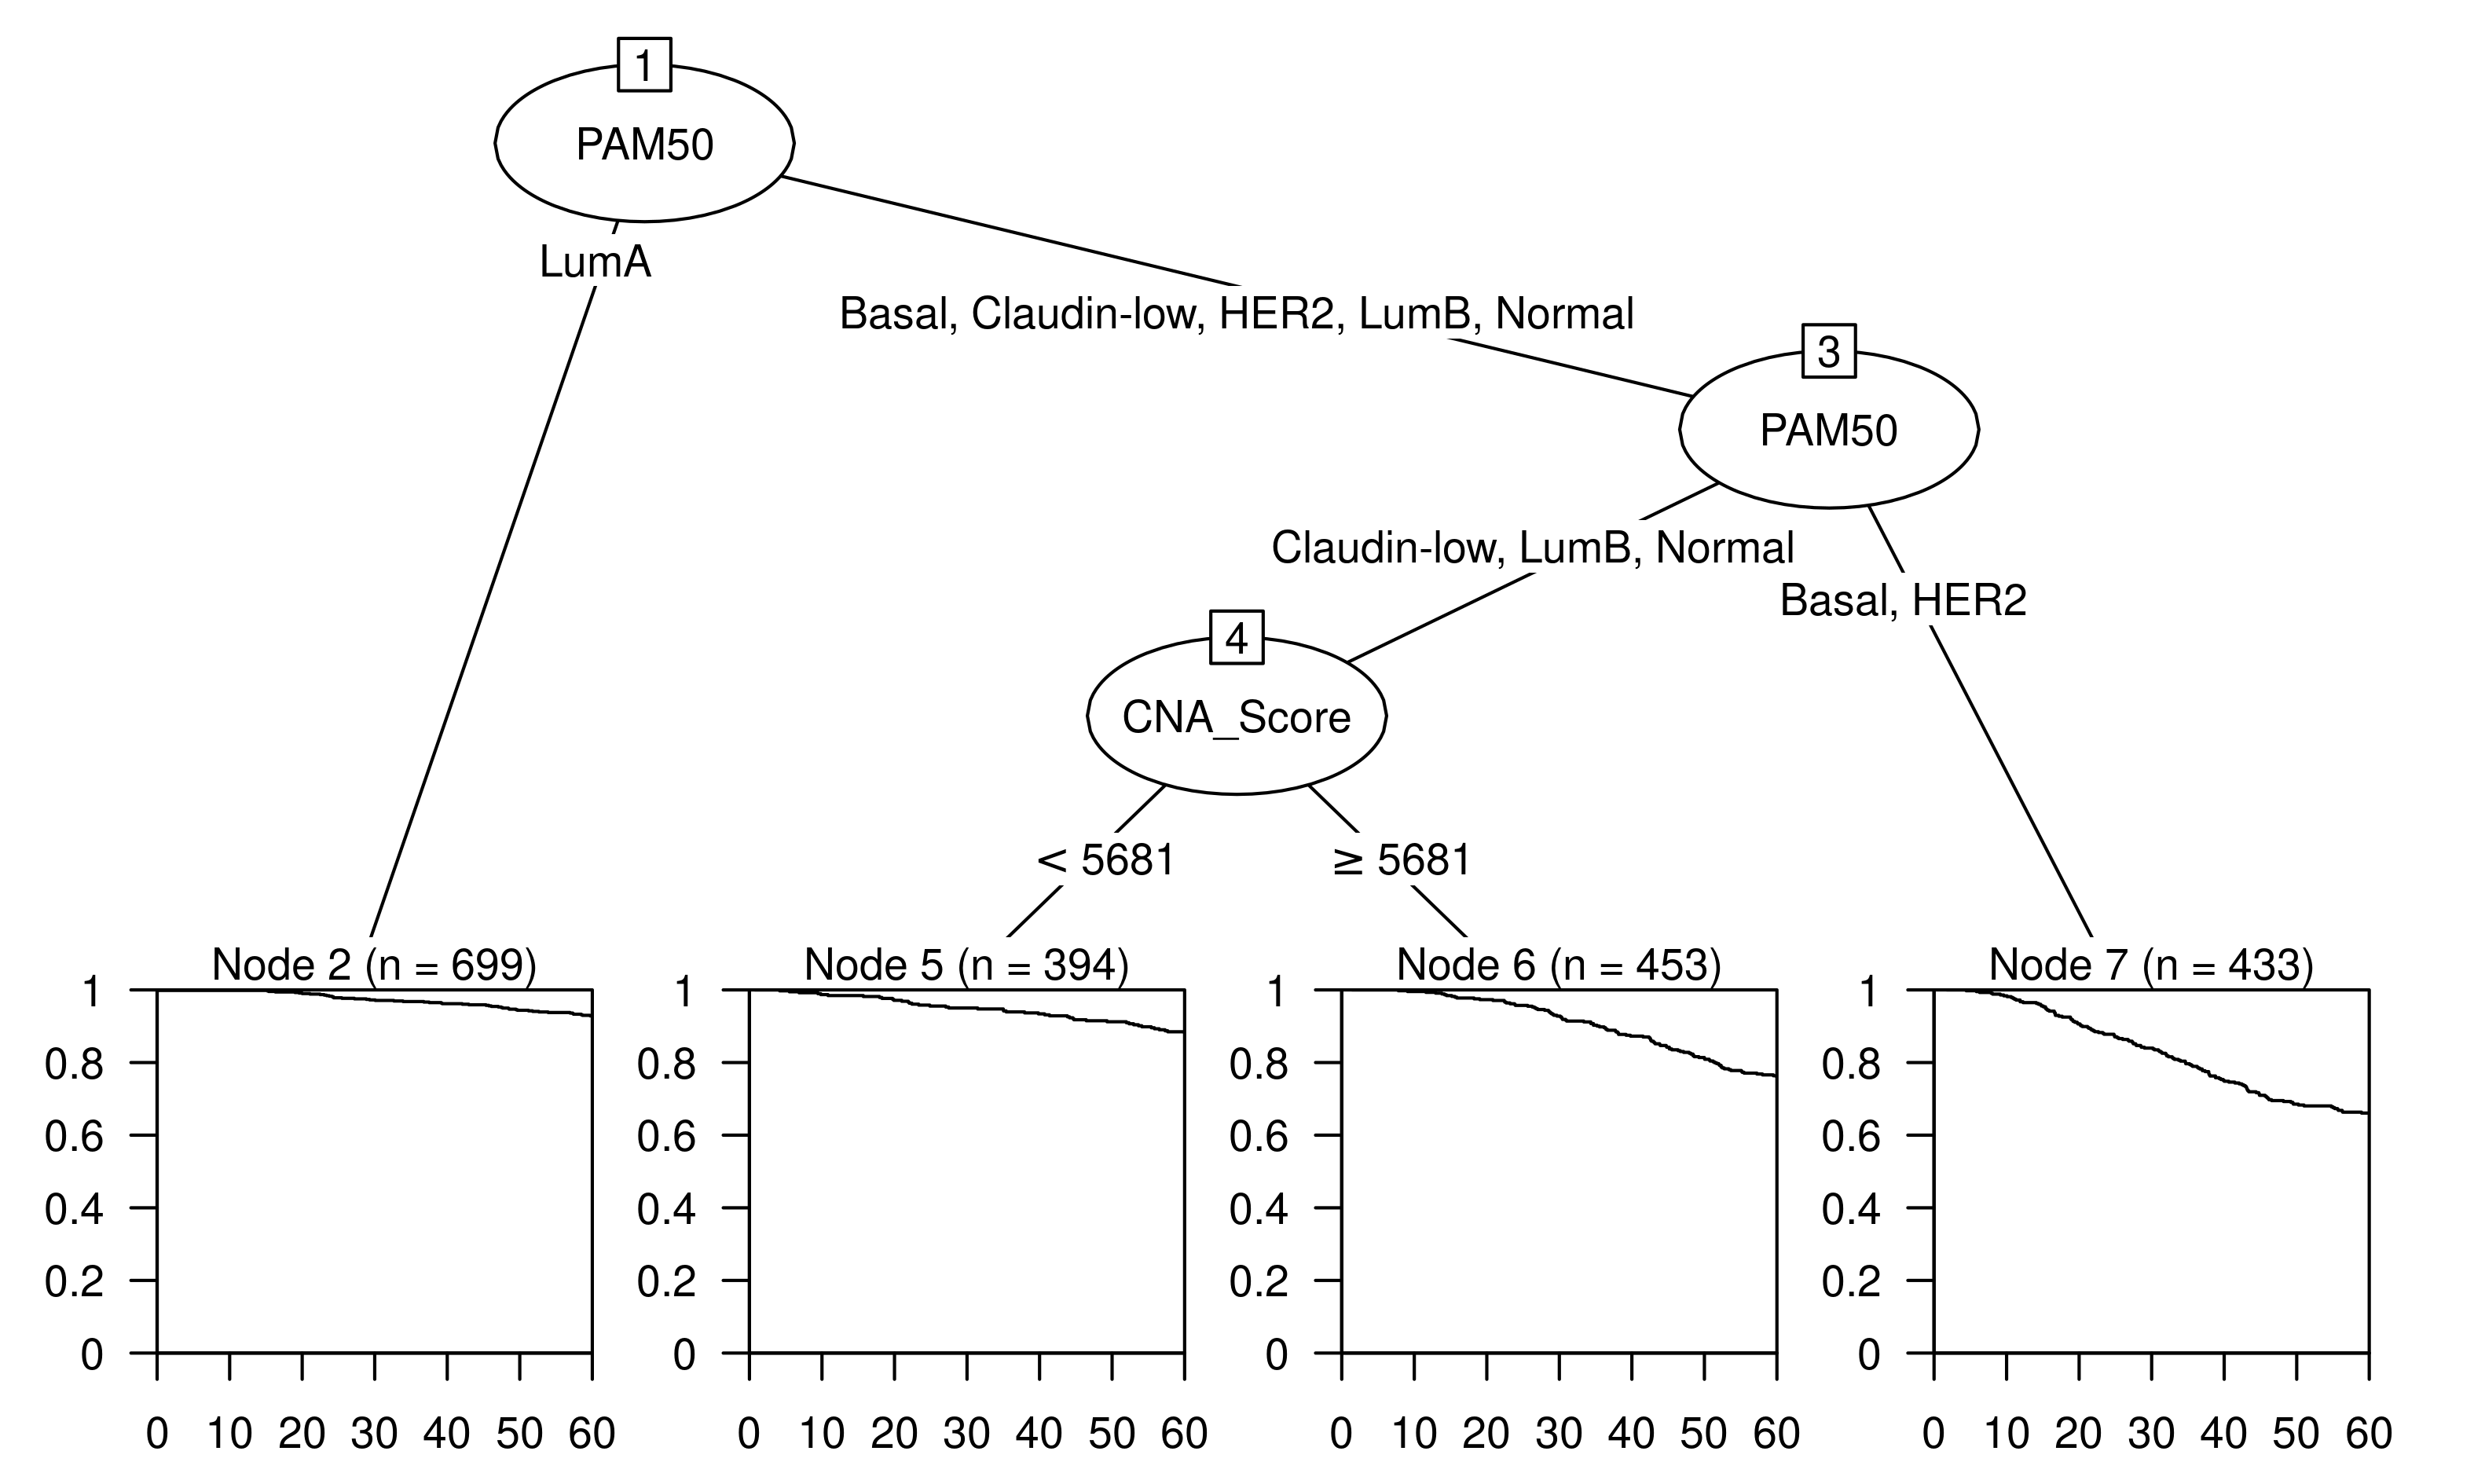
\includegraphics[width=1\textwidth]{../figures/Chapter_3/PartyKit_Survival_Score_FiveYearDSS_PAM50.png}
\end{subfigure}

\vspace{2cm}

\begin{subfigure}{\textwidth}
\subcaption{}
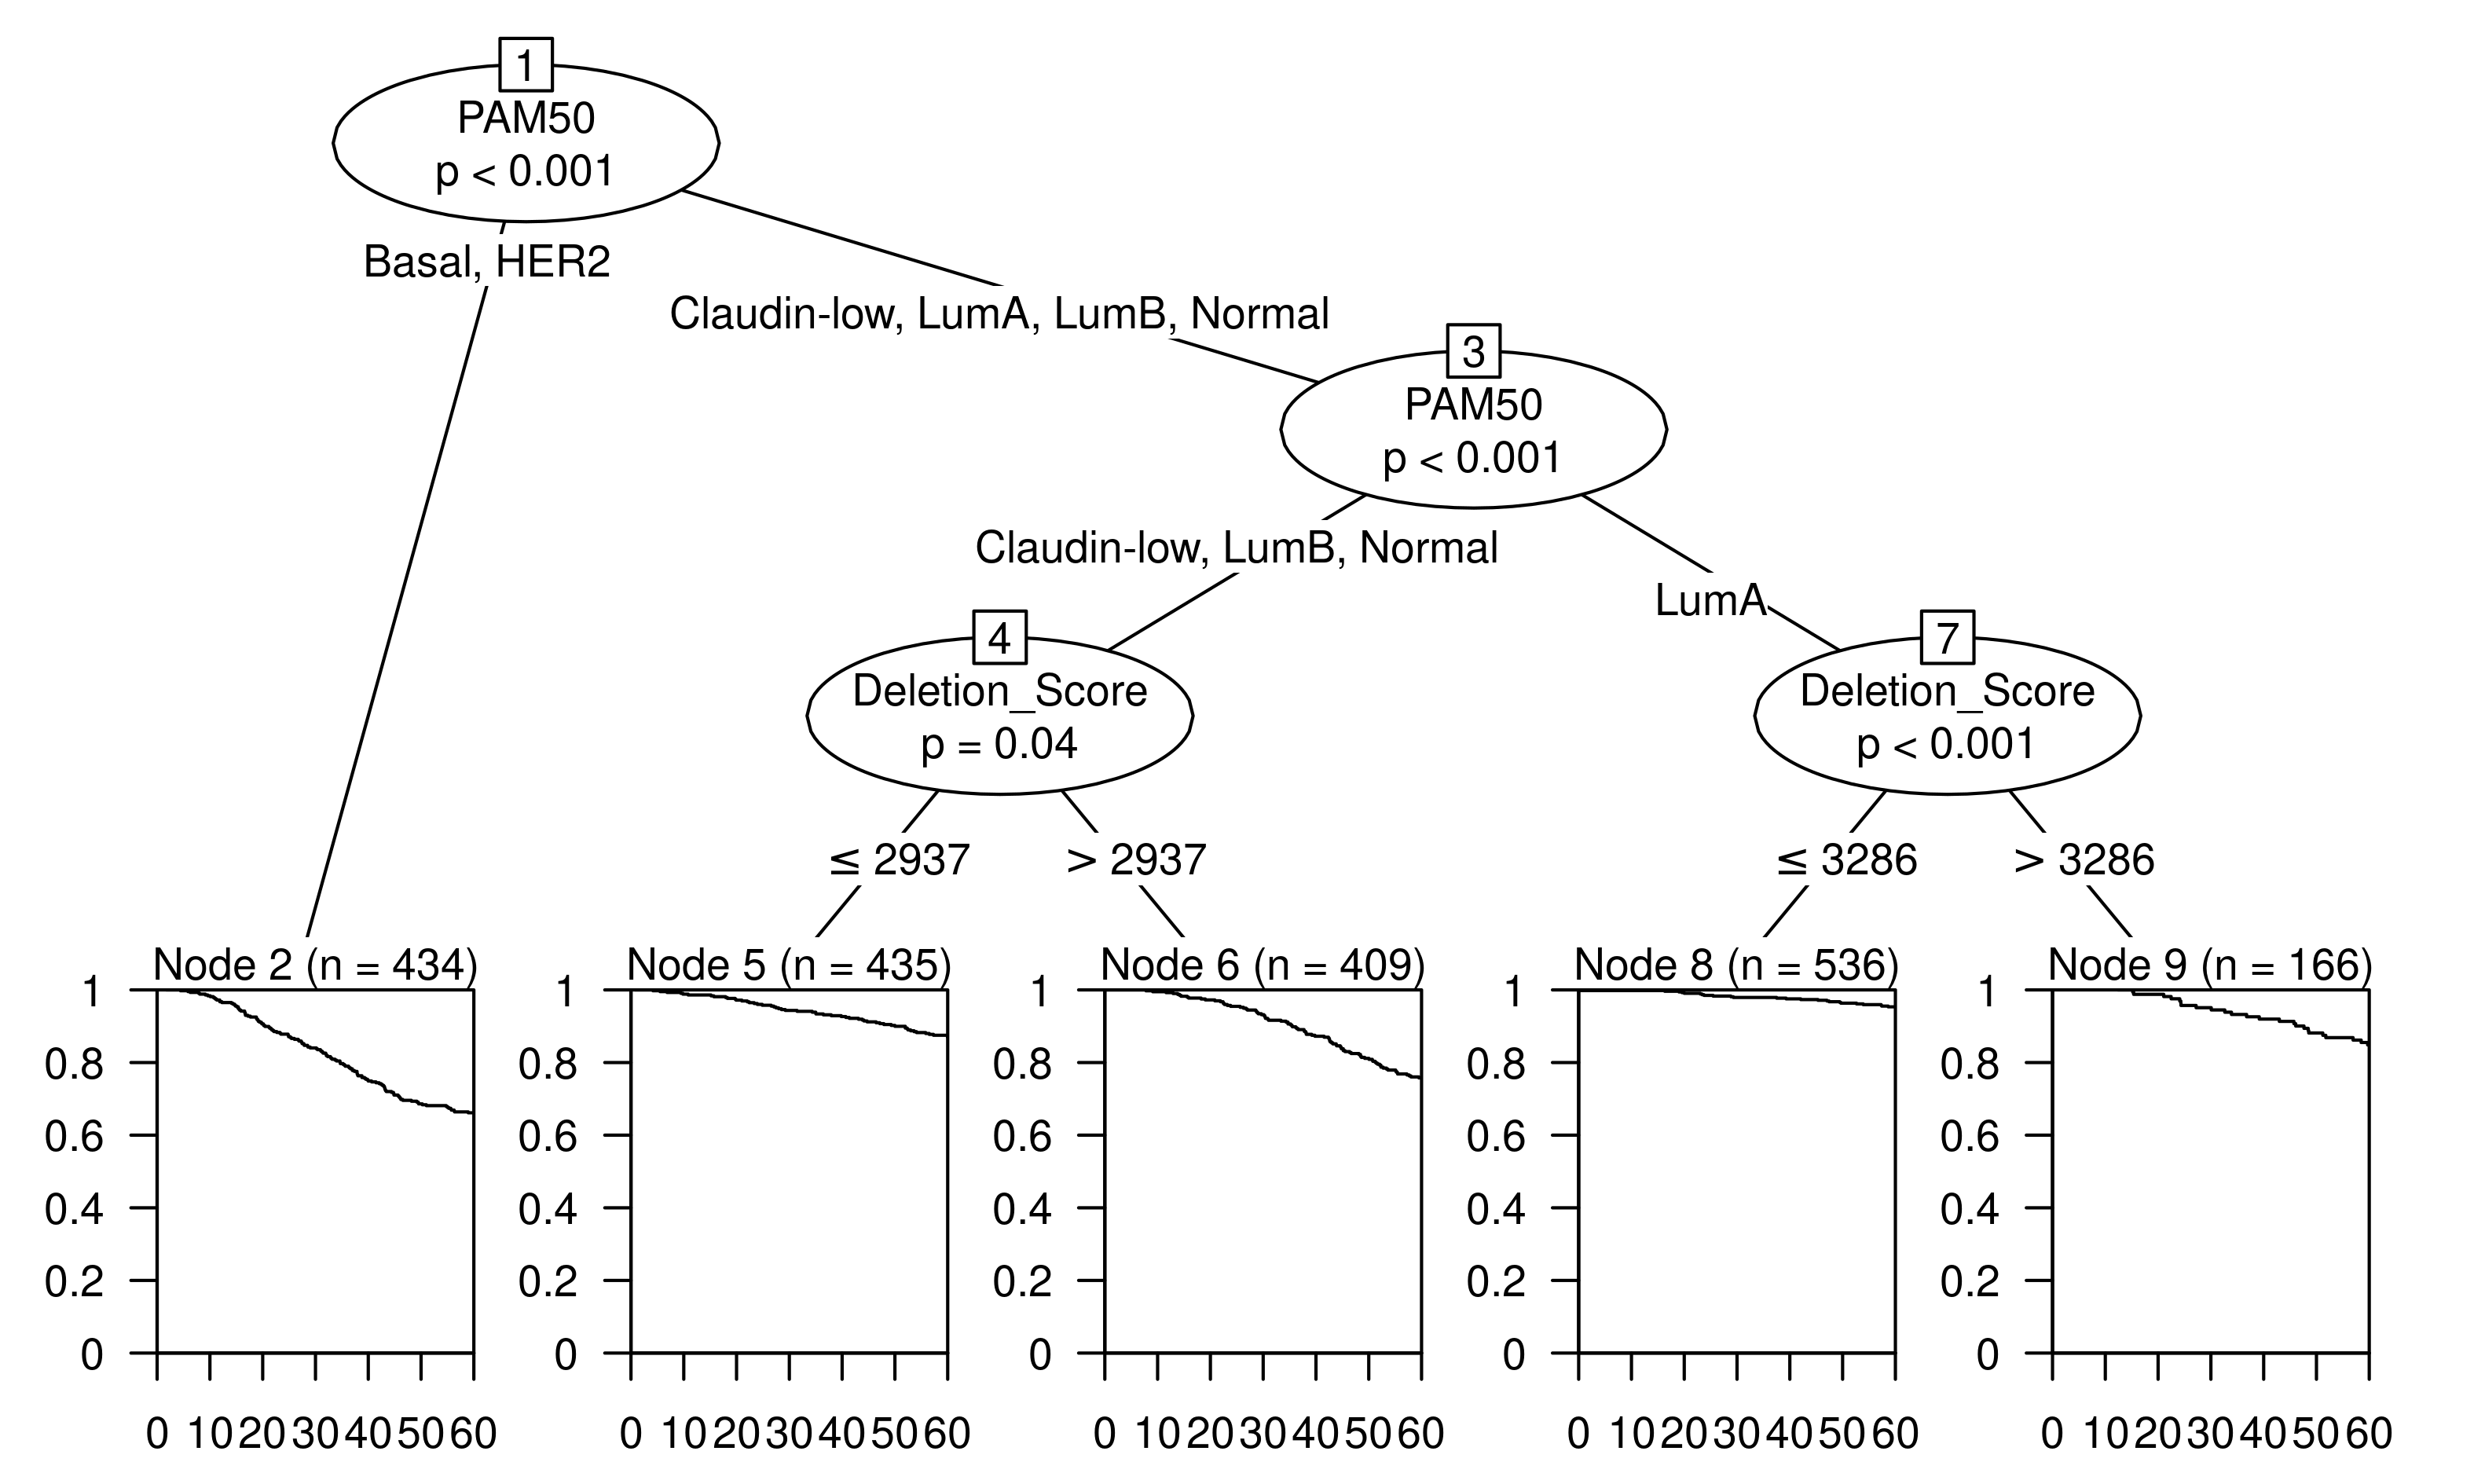
\includegraphics[width=1\textwidth]{../figures/Chapter_3/Ctree_Survival_Score_FiveYearDSS_PAM50.png}
\end{subfigure}

\vspace{0.5cm}

\caption[Recursive partitioning survival trees for five-year disease-specific survival using PAM50 subtype and the six CNA Score metrics as candidate predictors.]{Recursive partitioning survival trees for five-year disease-specific survival using PAM50 subtype and the six CNA Score metrics as candidate predictors. (A) Trees fitted using the rpart algorithm and (B) trees fitted using the ctree algorithm.}
\label{fig:PAM50_CNA_Score_FiveYearDSS}
\end{figure}

\begin{figure}[!h]
\centering

\vspace{0.5cm}

\begin{subfigure}{\textwidth}
\subcaption{}
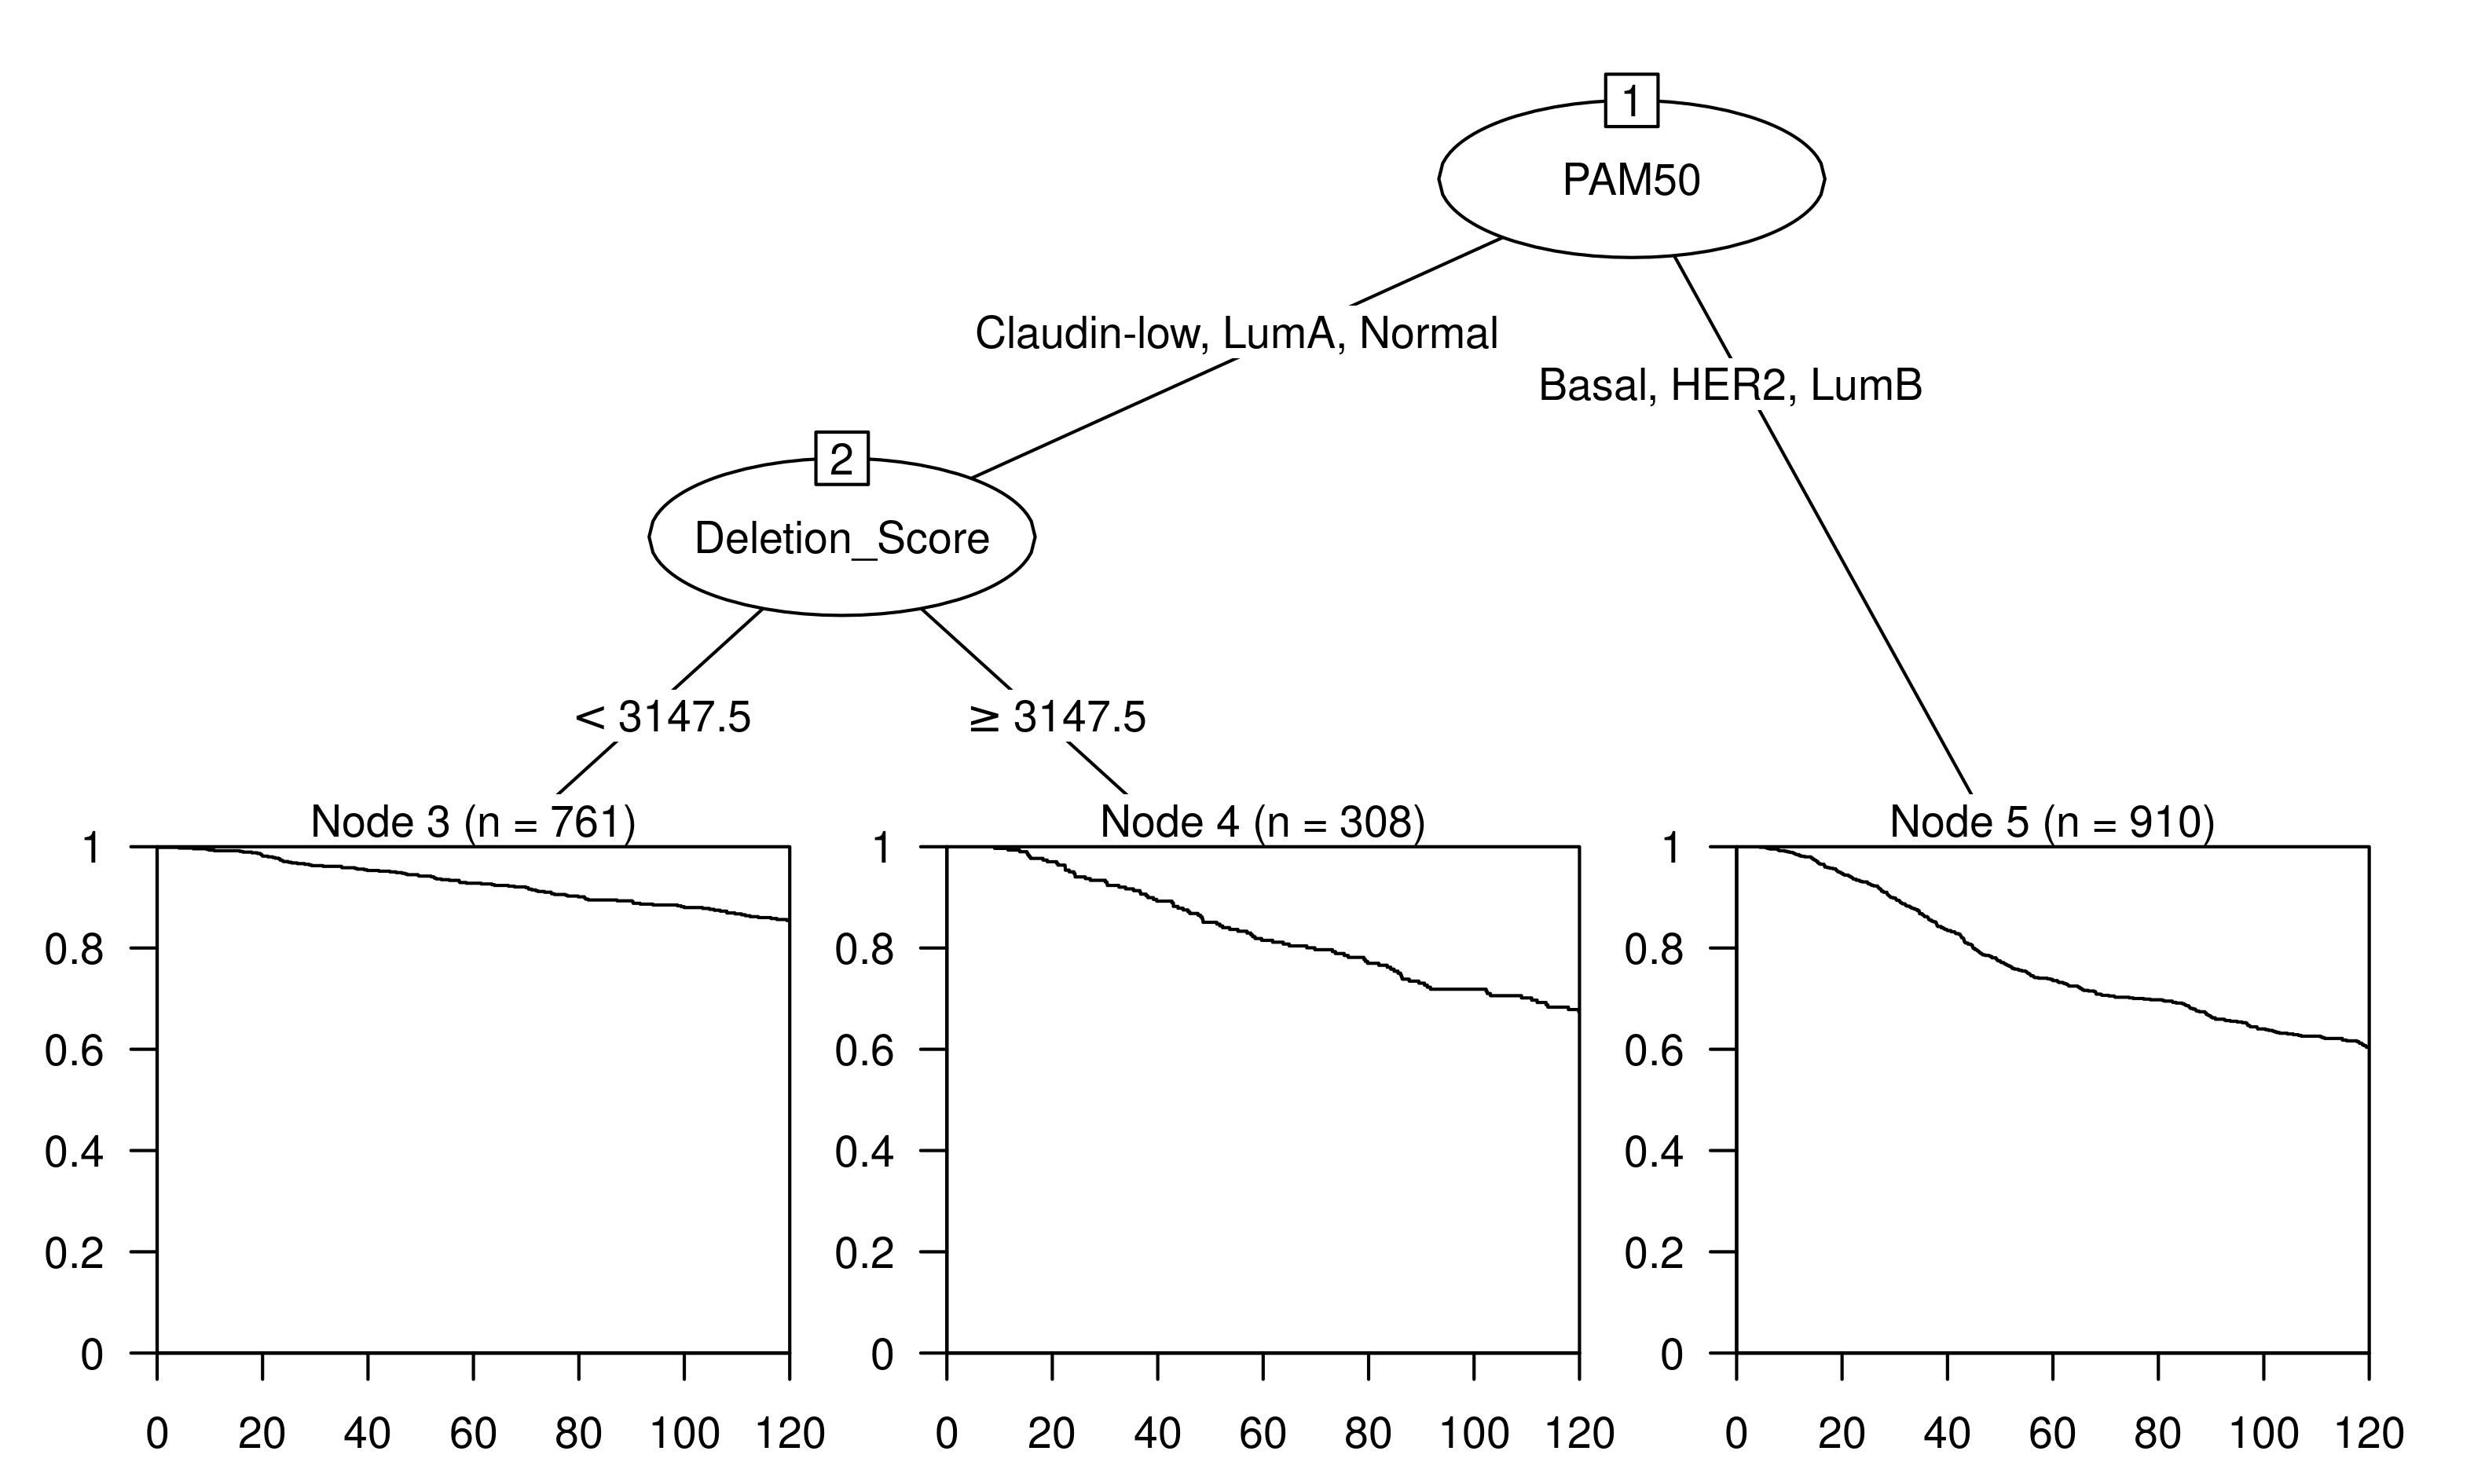
\includegraphics[width=1\textwidth]{../figures/Chapter_3/PartyKit_Survival_Score_TenYearDSS_PAM50.png}
\end{subfigure}

\vspace{2cm}

\begin{subfigure}{\textwidth}
\subcaption{}
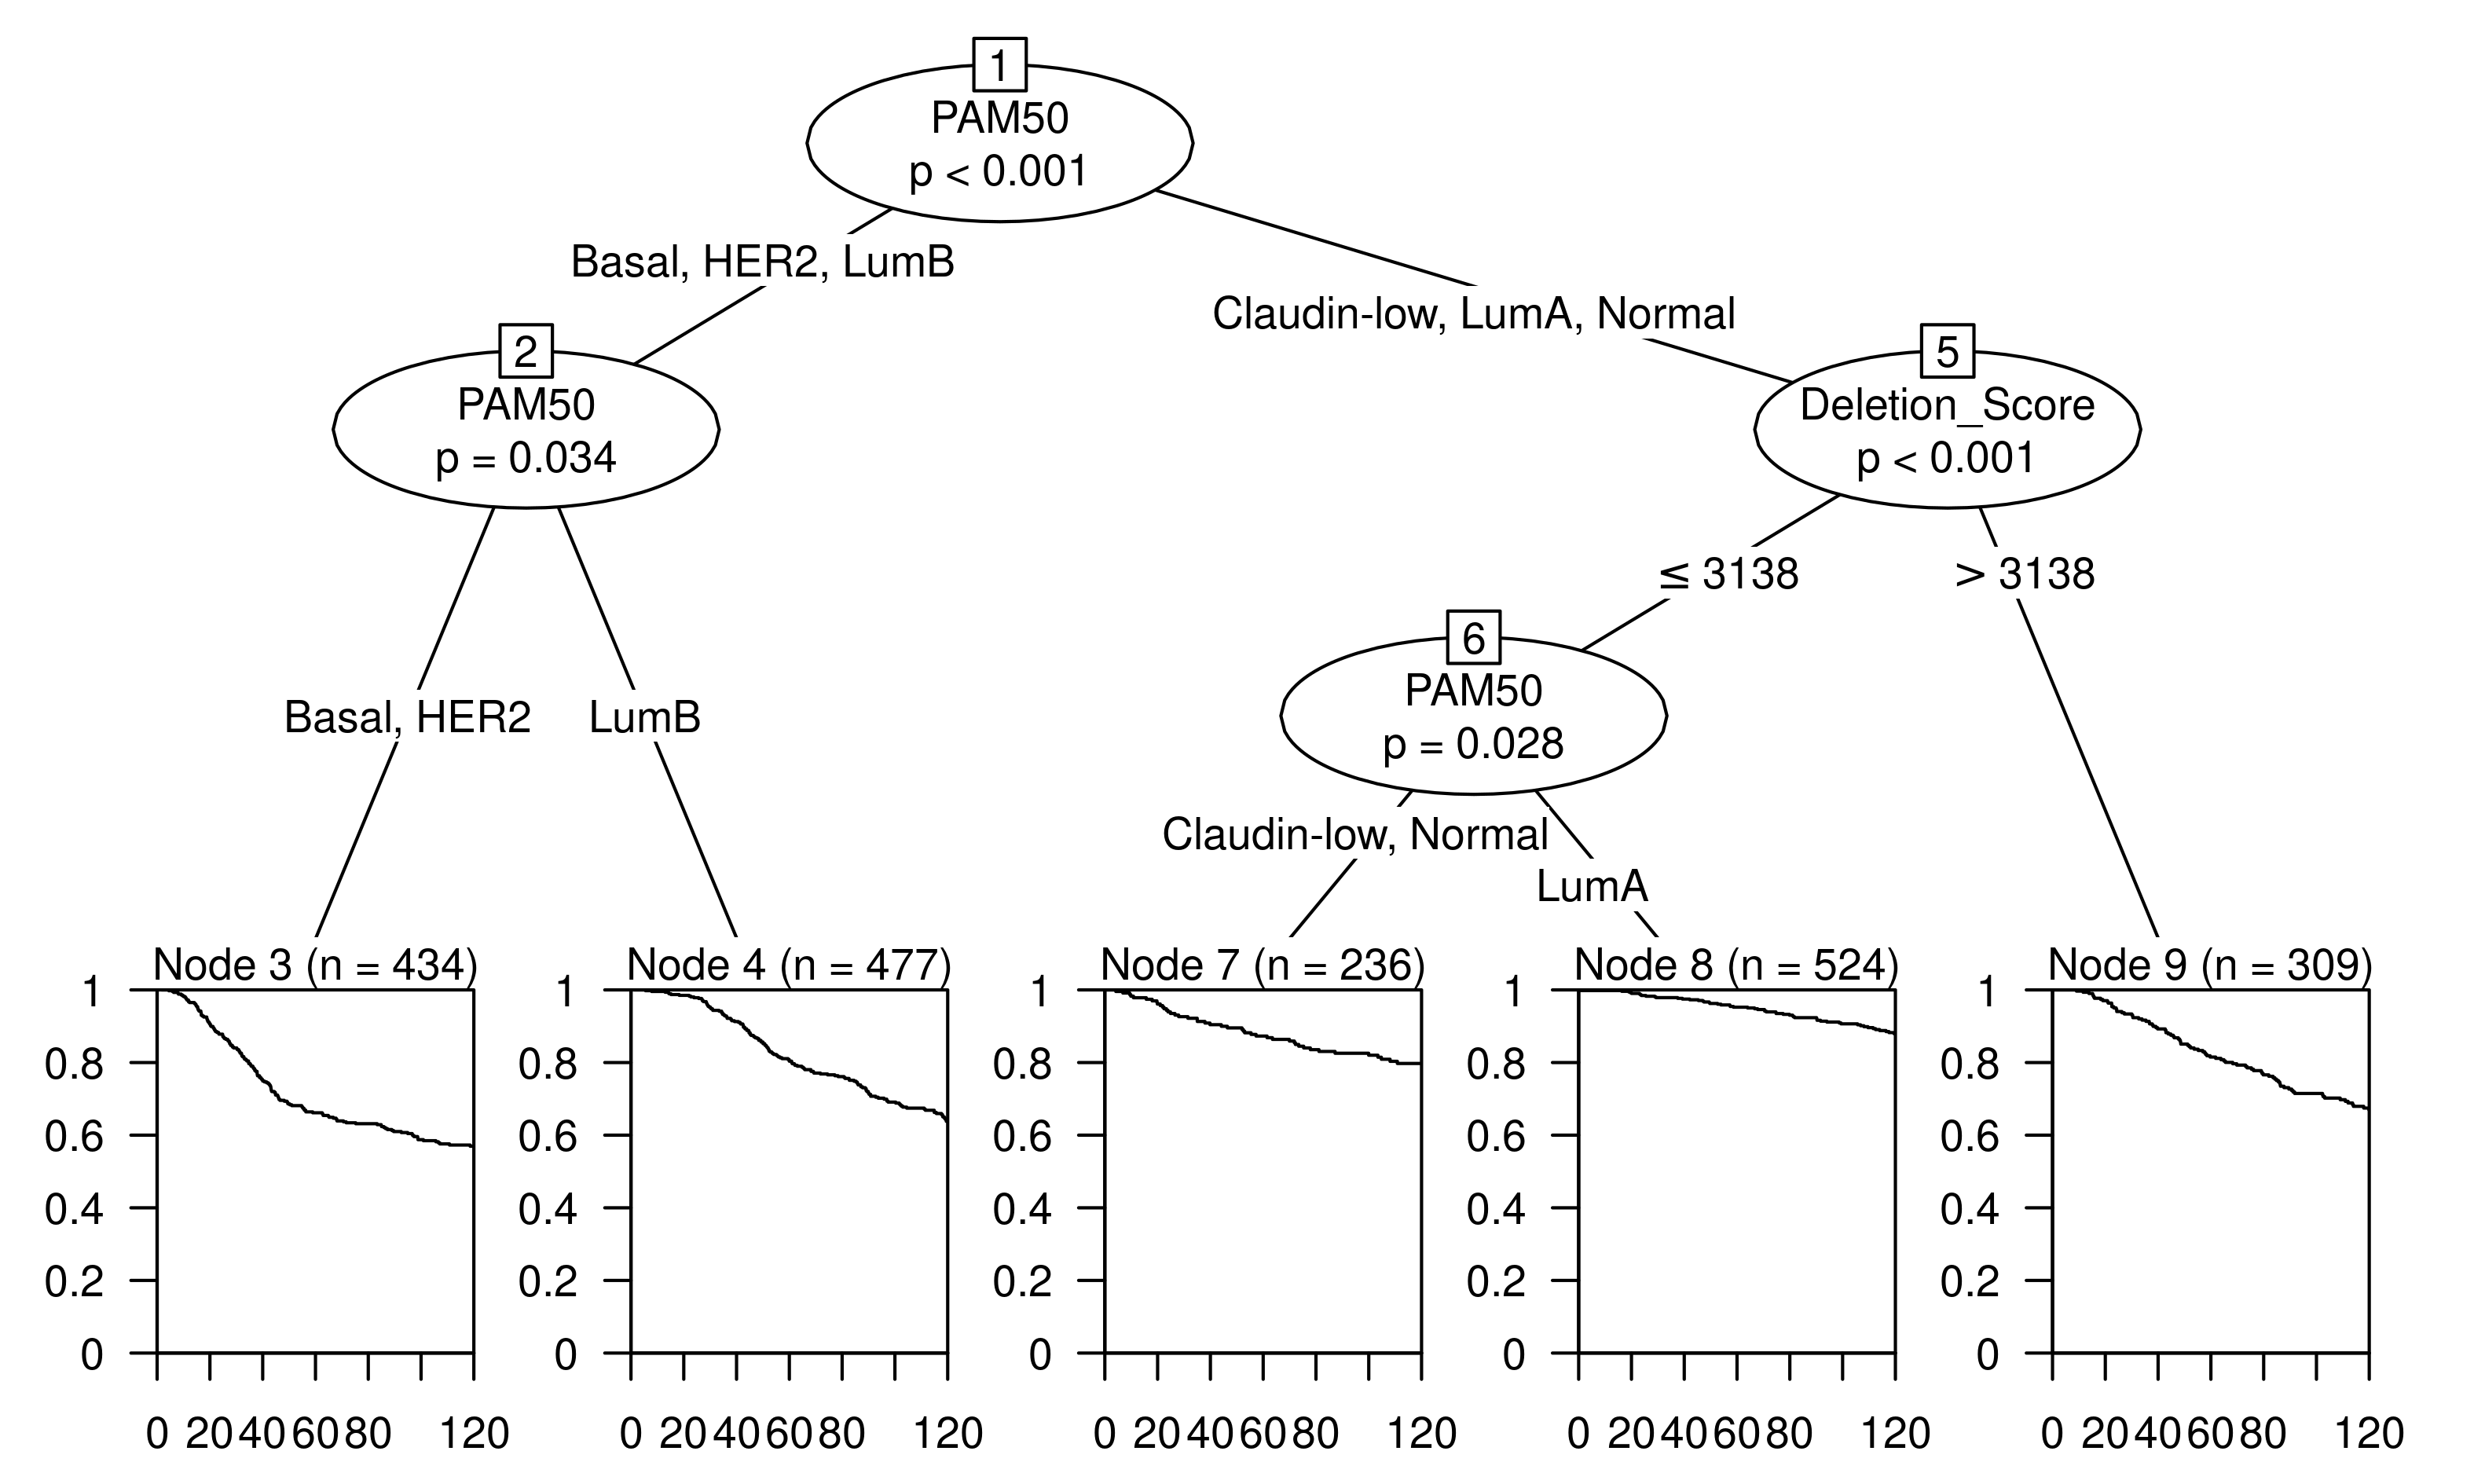
\includegraphics[width=1\textwidth]{../figures/Chapter_3/Ctree_Survival_Score_TenYearDSS_PAM50.png}
\end{subfigure}

\vspace{0.5cm}

\caption[Recursive partitioning survival trees for ten-year disease-specific survival using PAM50 subtype and the six CNA Score metrics as candidate predictors.]{Recursive partitioning survival trees for ten-year disease-specific survival using PAM50 subtype and the six CNA Score metrics as candidate predictors. (A) Trees fitted using the rpart algorithm and (B) trees fitted using the ctree algorithm.}
\label{fig:PAM50_CNA_Score_TenYearDSS}
\end{figure}


\begin{figure}[!h]
\centering

\vspace{0.5cm}

\begin{subfigure}{\textwidth}
\subcaption{}
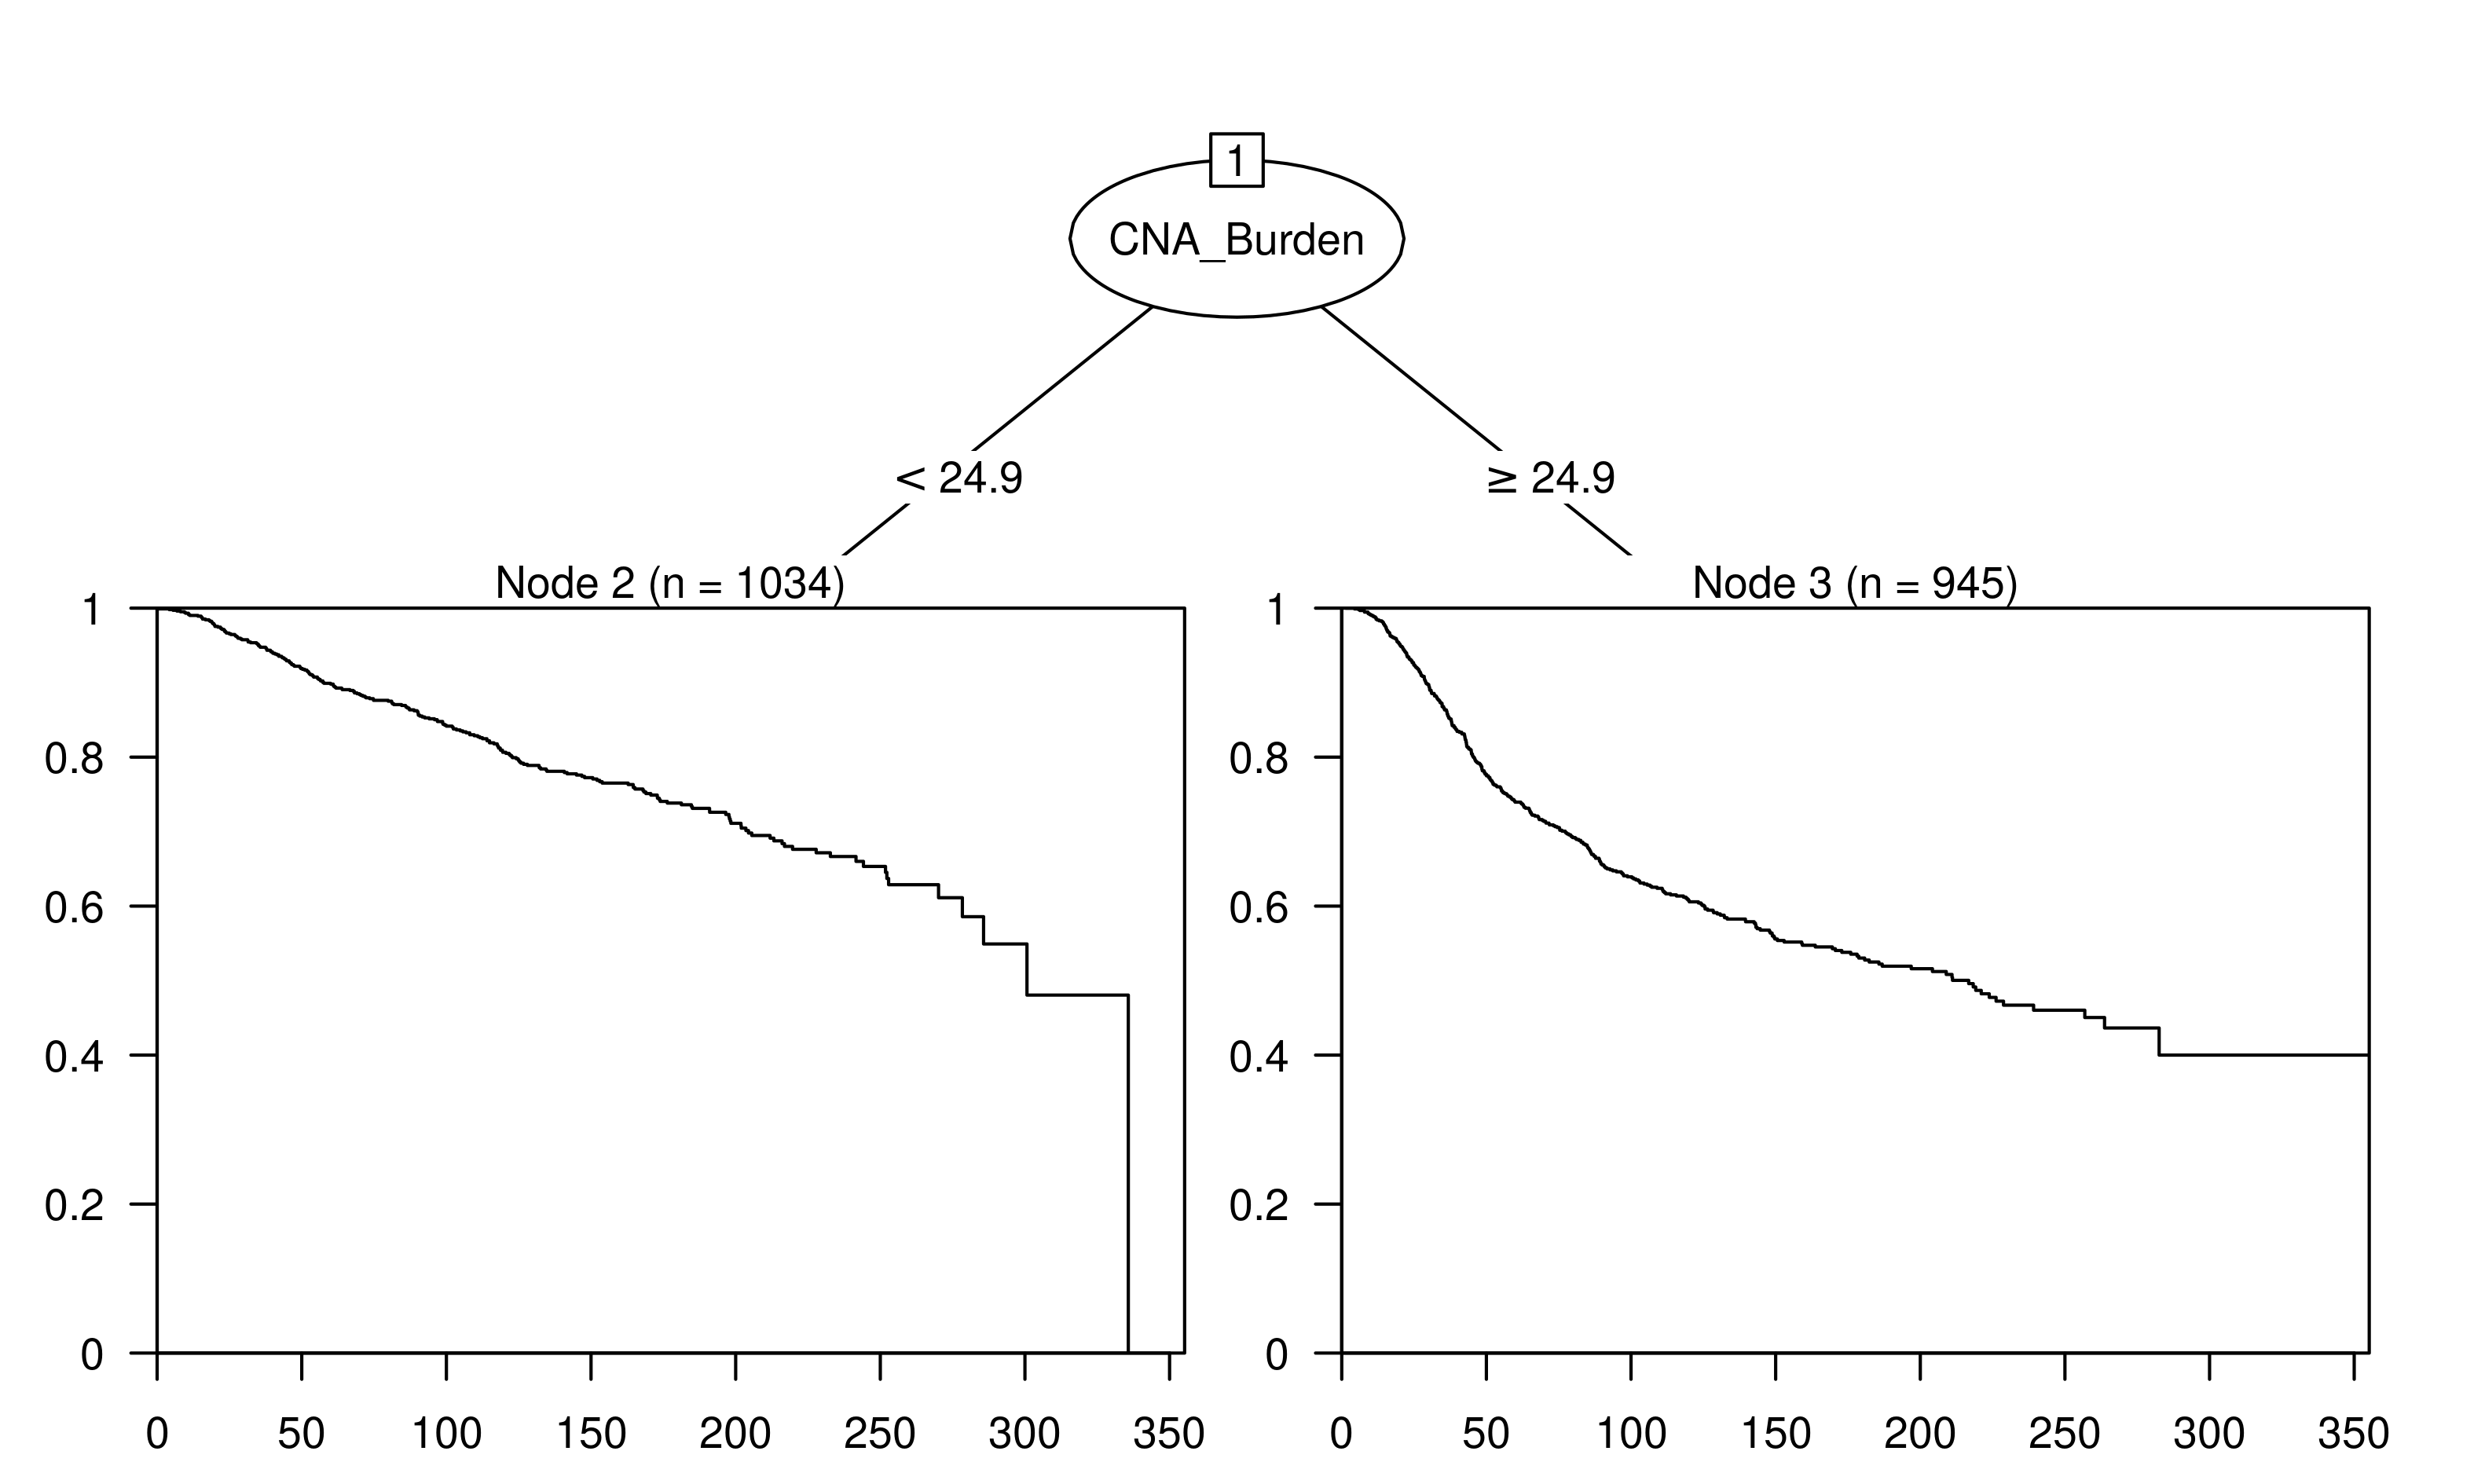
\includegraphics[width=1\textwidth]{../figures/Chapter_3/PartyKit_Survival_Burden_DSS_PAM50.png}
\end{subfigure}
\vspace{2cm}

\begin{subfigure}{\textwidth}
\subcaption{}
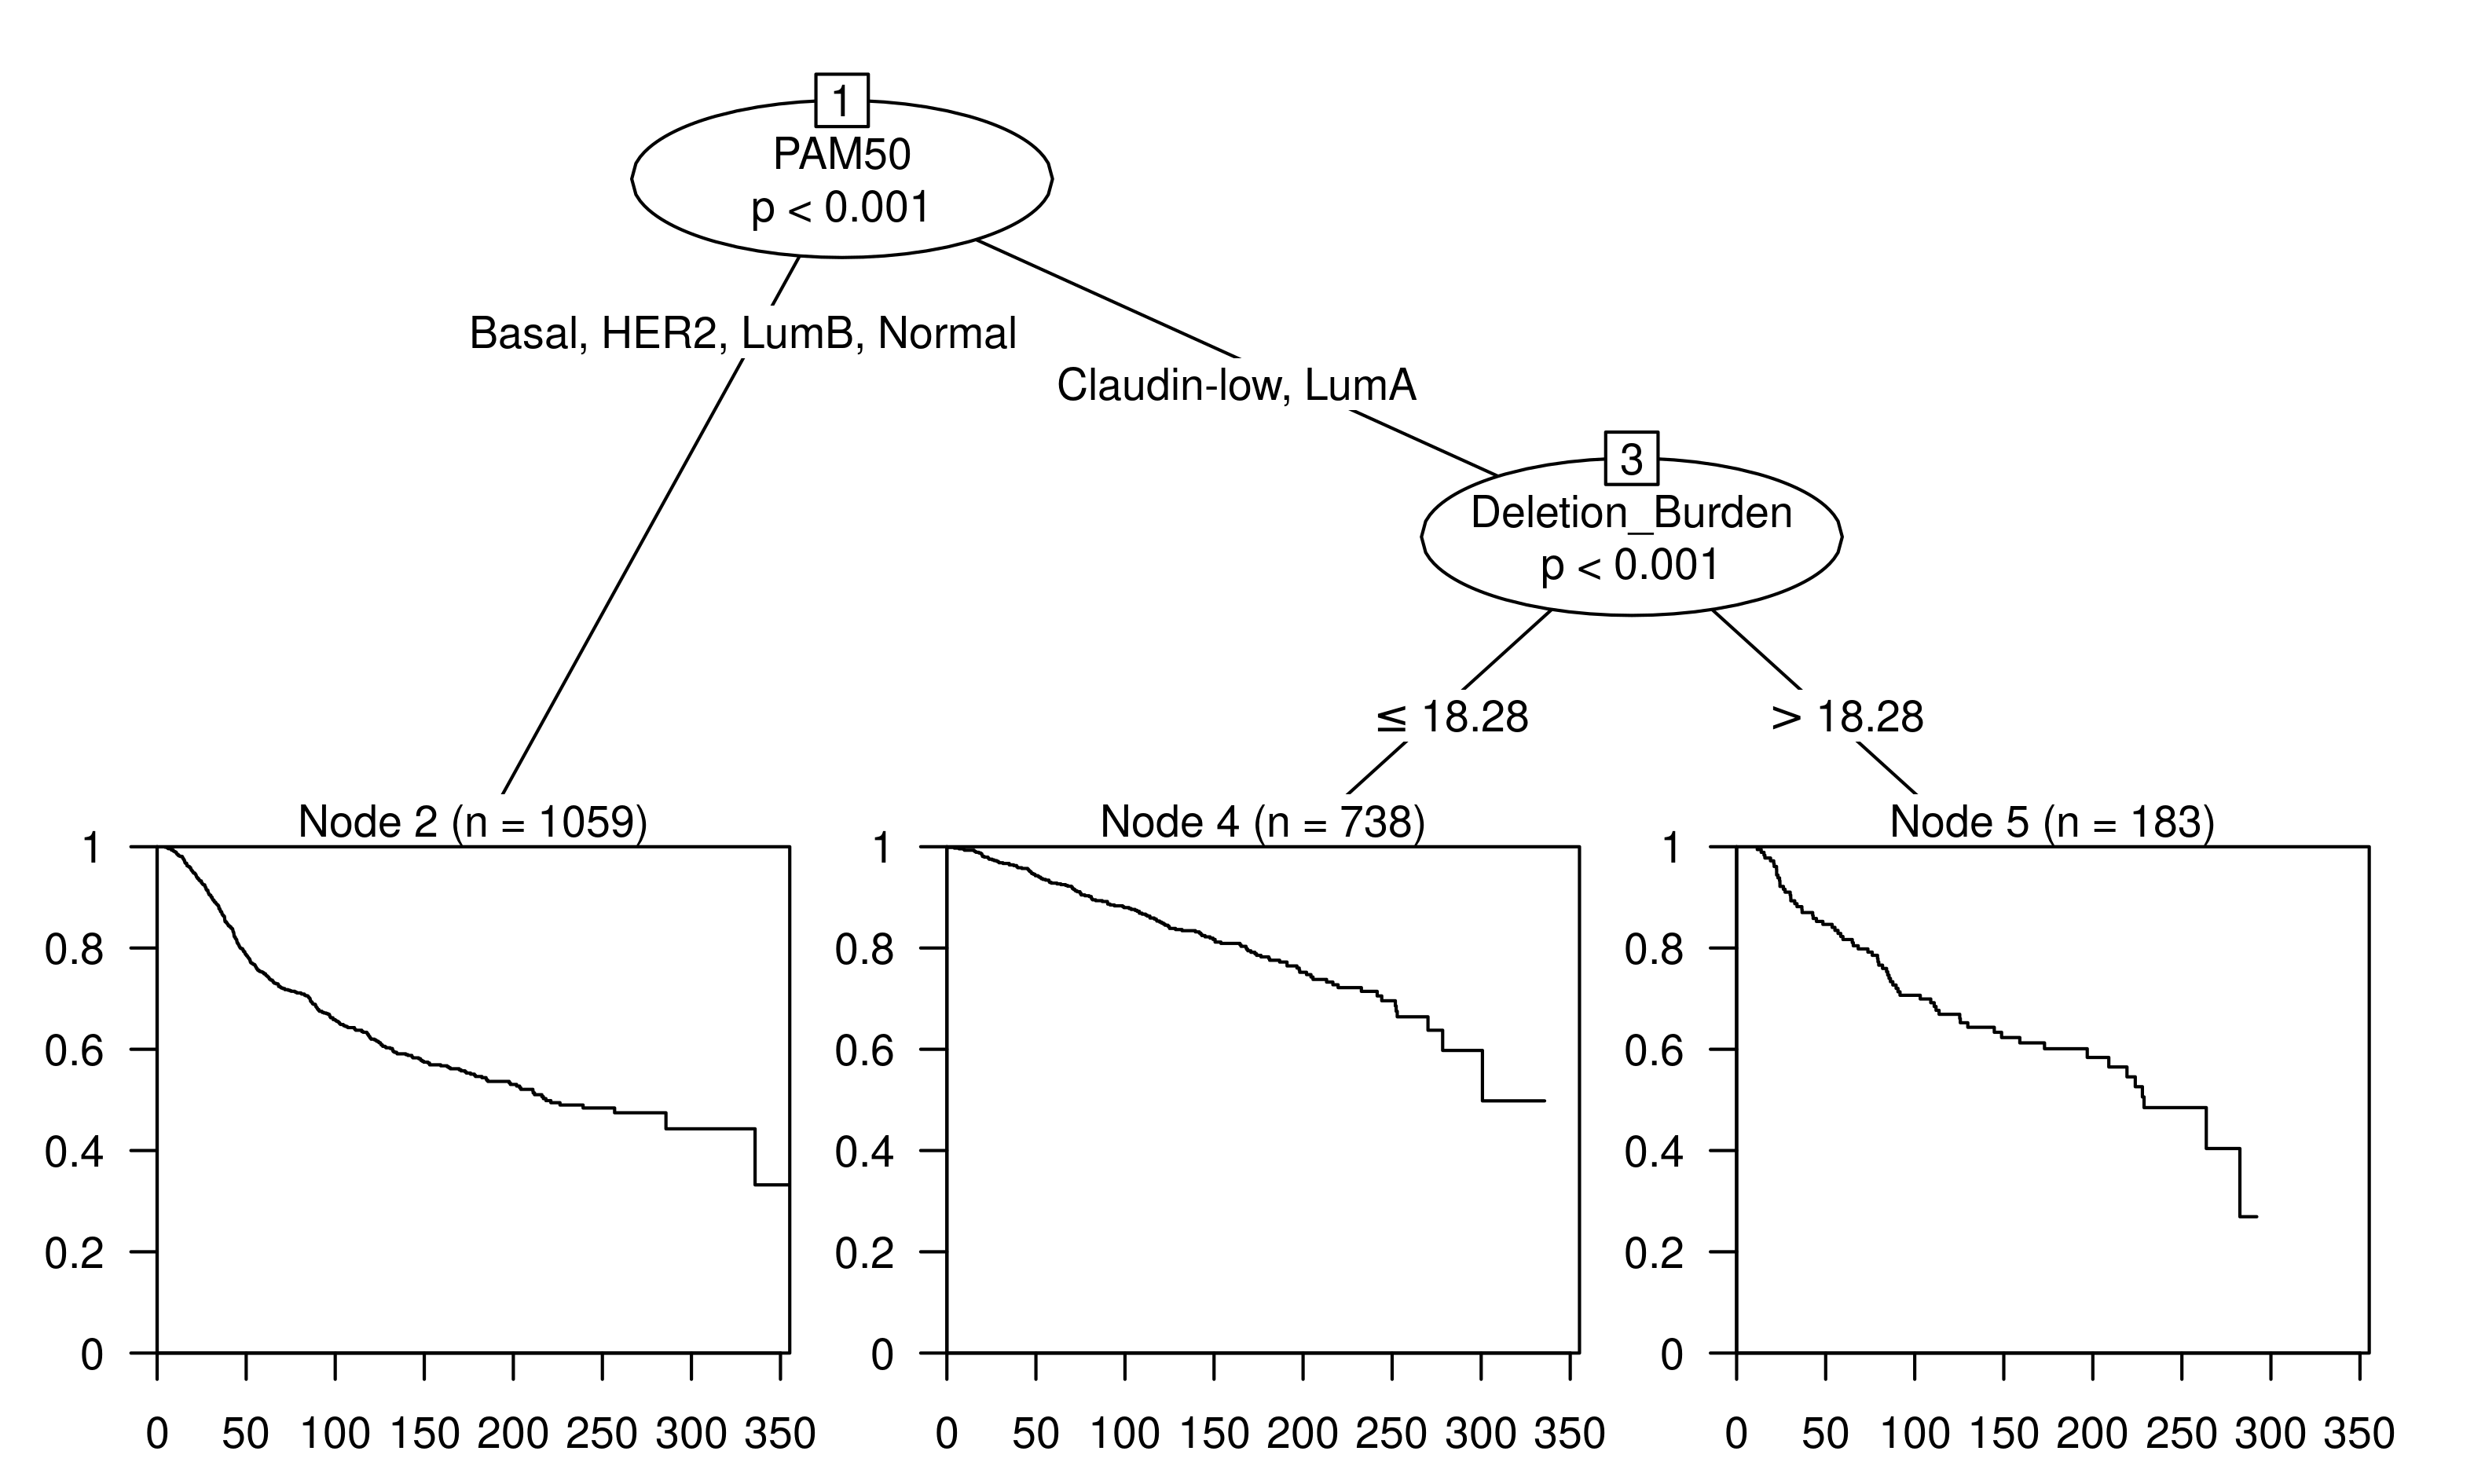
\includegraphics[width=1\textwidth]{../figures/Chapter_3/Ctree_Survival_Burden_DSS_PAM50.png}
\end{subfigure}
\vspace{0.5cm}

\caption[Recursive partitioning survival trees for disease-specific survival using PAM50 subtype and the six CNA Burden metrics as candidate predictors.]{Recursive partitioning survival trees for disease-specific survival using PAM50 subtype and the six CNA Burden metrics as candidate predictors. (A) Trees fitted using the rpart algorithm and (B) trees fitted using the ctree algorithm.}
\label{fig:PAM50_CNA_Burden_DSS}
\end{figure}

\begin{figure}[!h]
\centering

\vspace{0.5cm}

\begin{subfigure}{\textwidth}
\subcaption{}
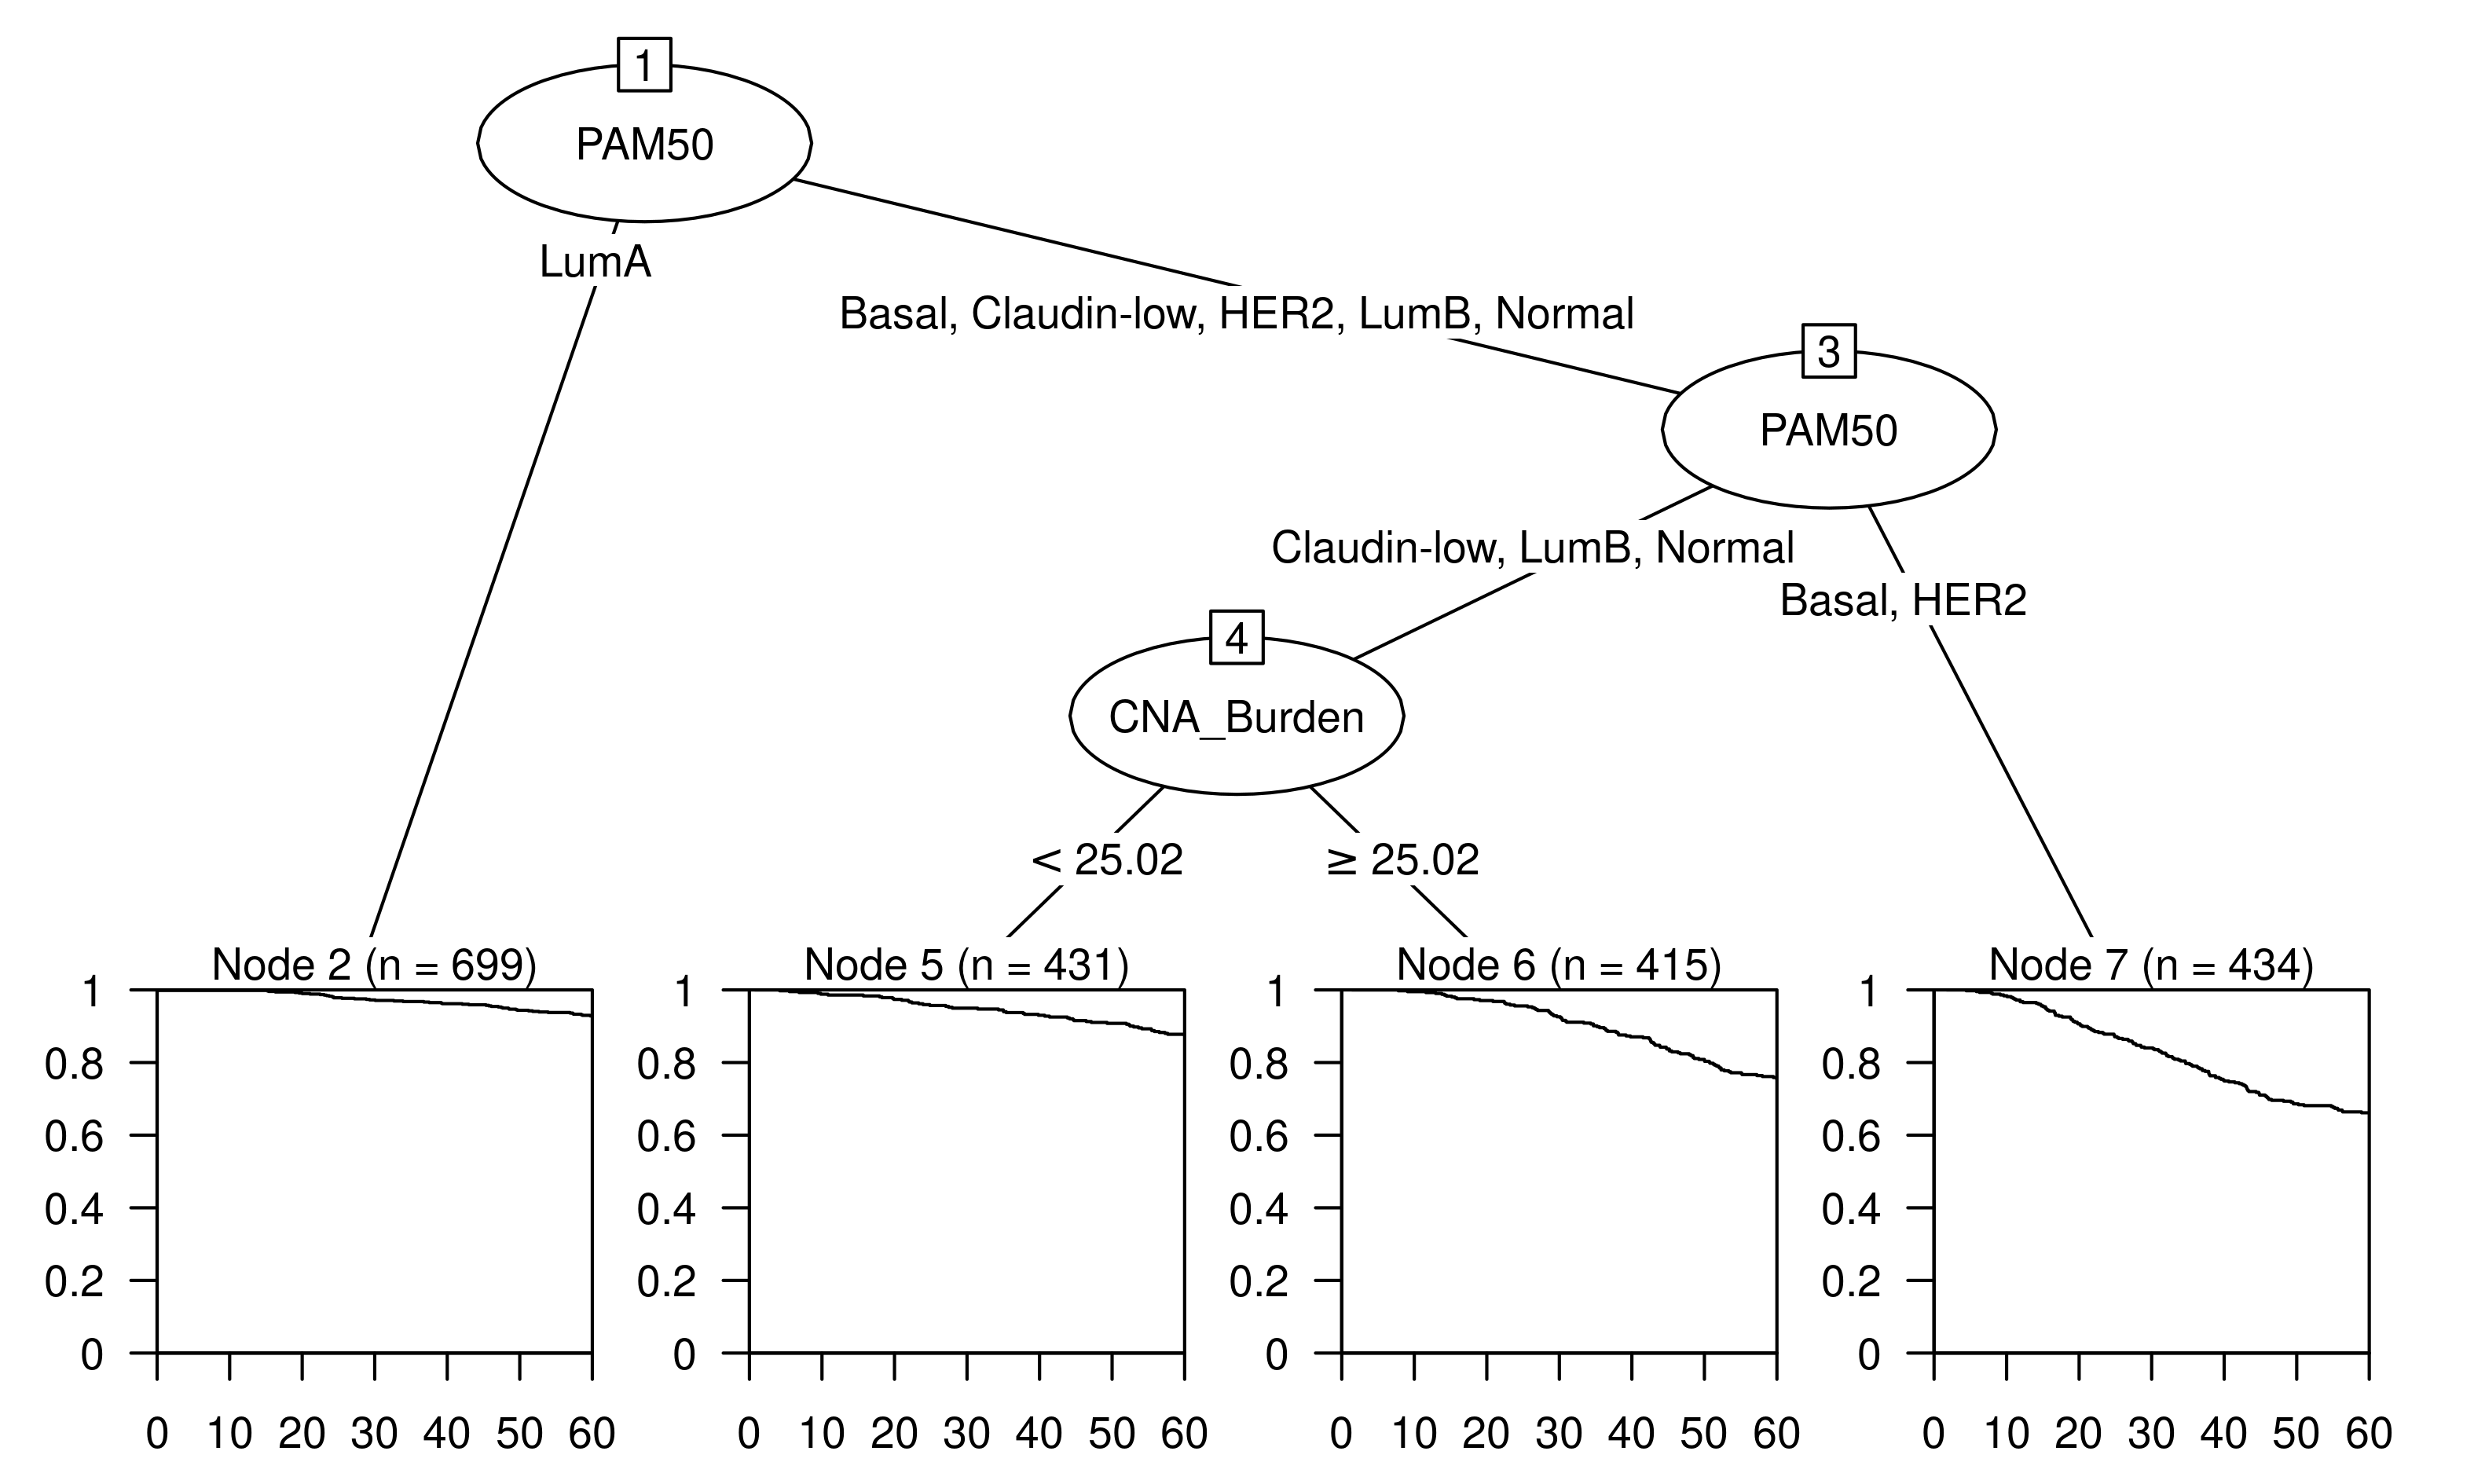
\includegraphics[width=1\textwidth]{../figures/Chapter_3/PartyKit_Survival_Burden_FiveYearDSS_PAM50.png}
\end{subfigure}
\vspace{2cm}


\begin{subfigure}{\textwidth}
\subcaption{}
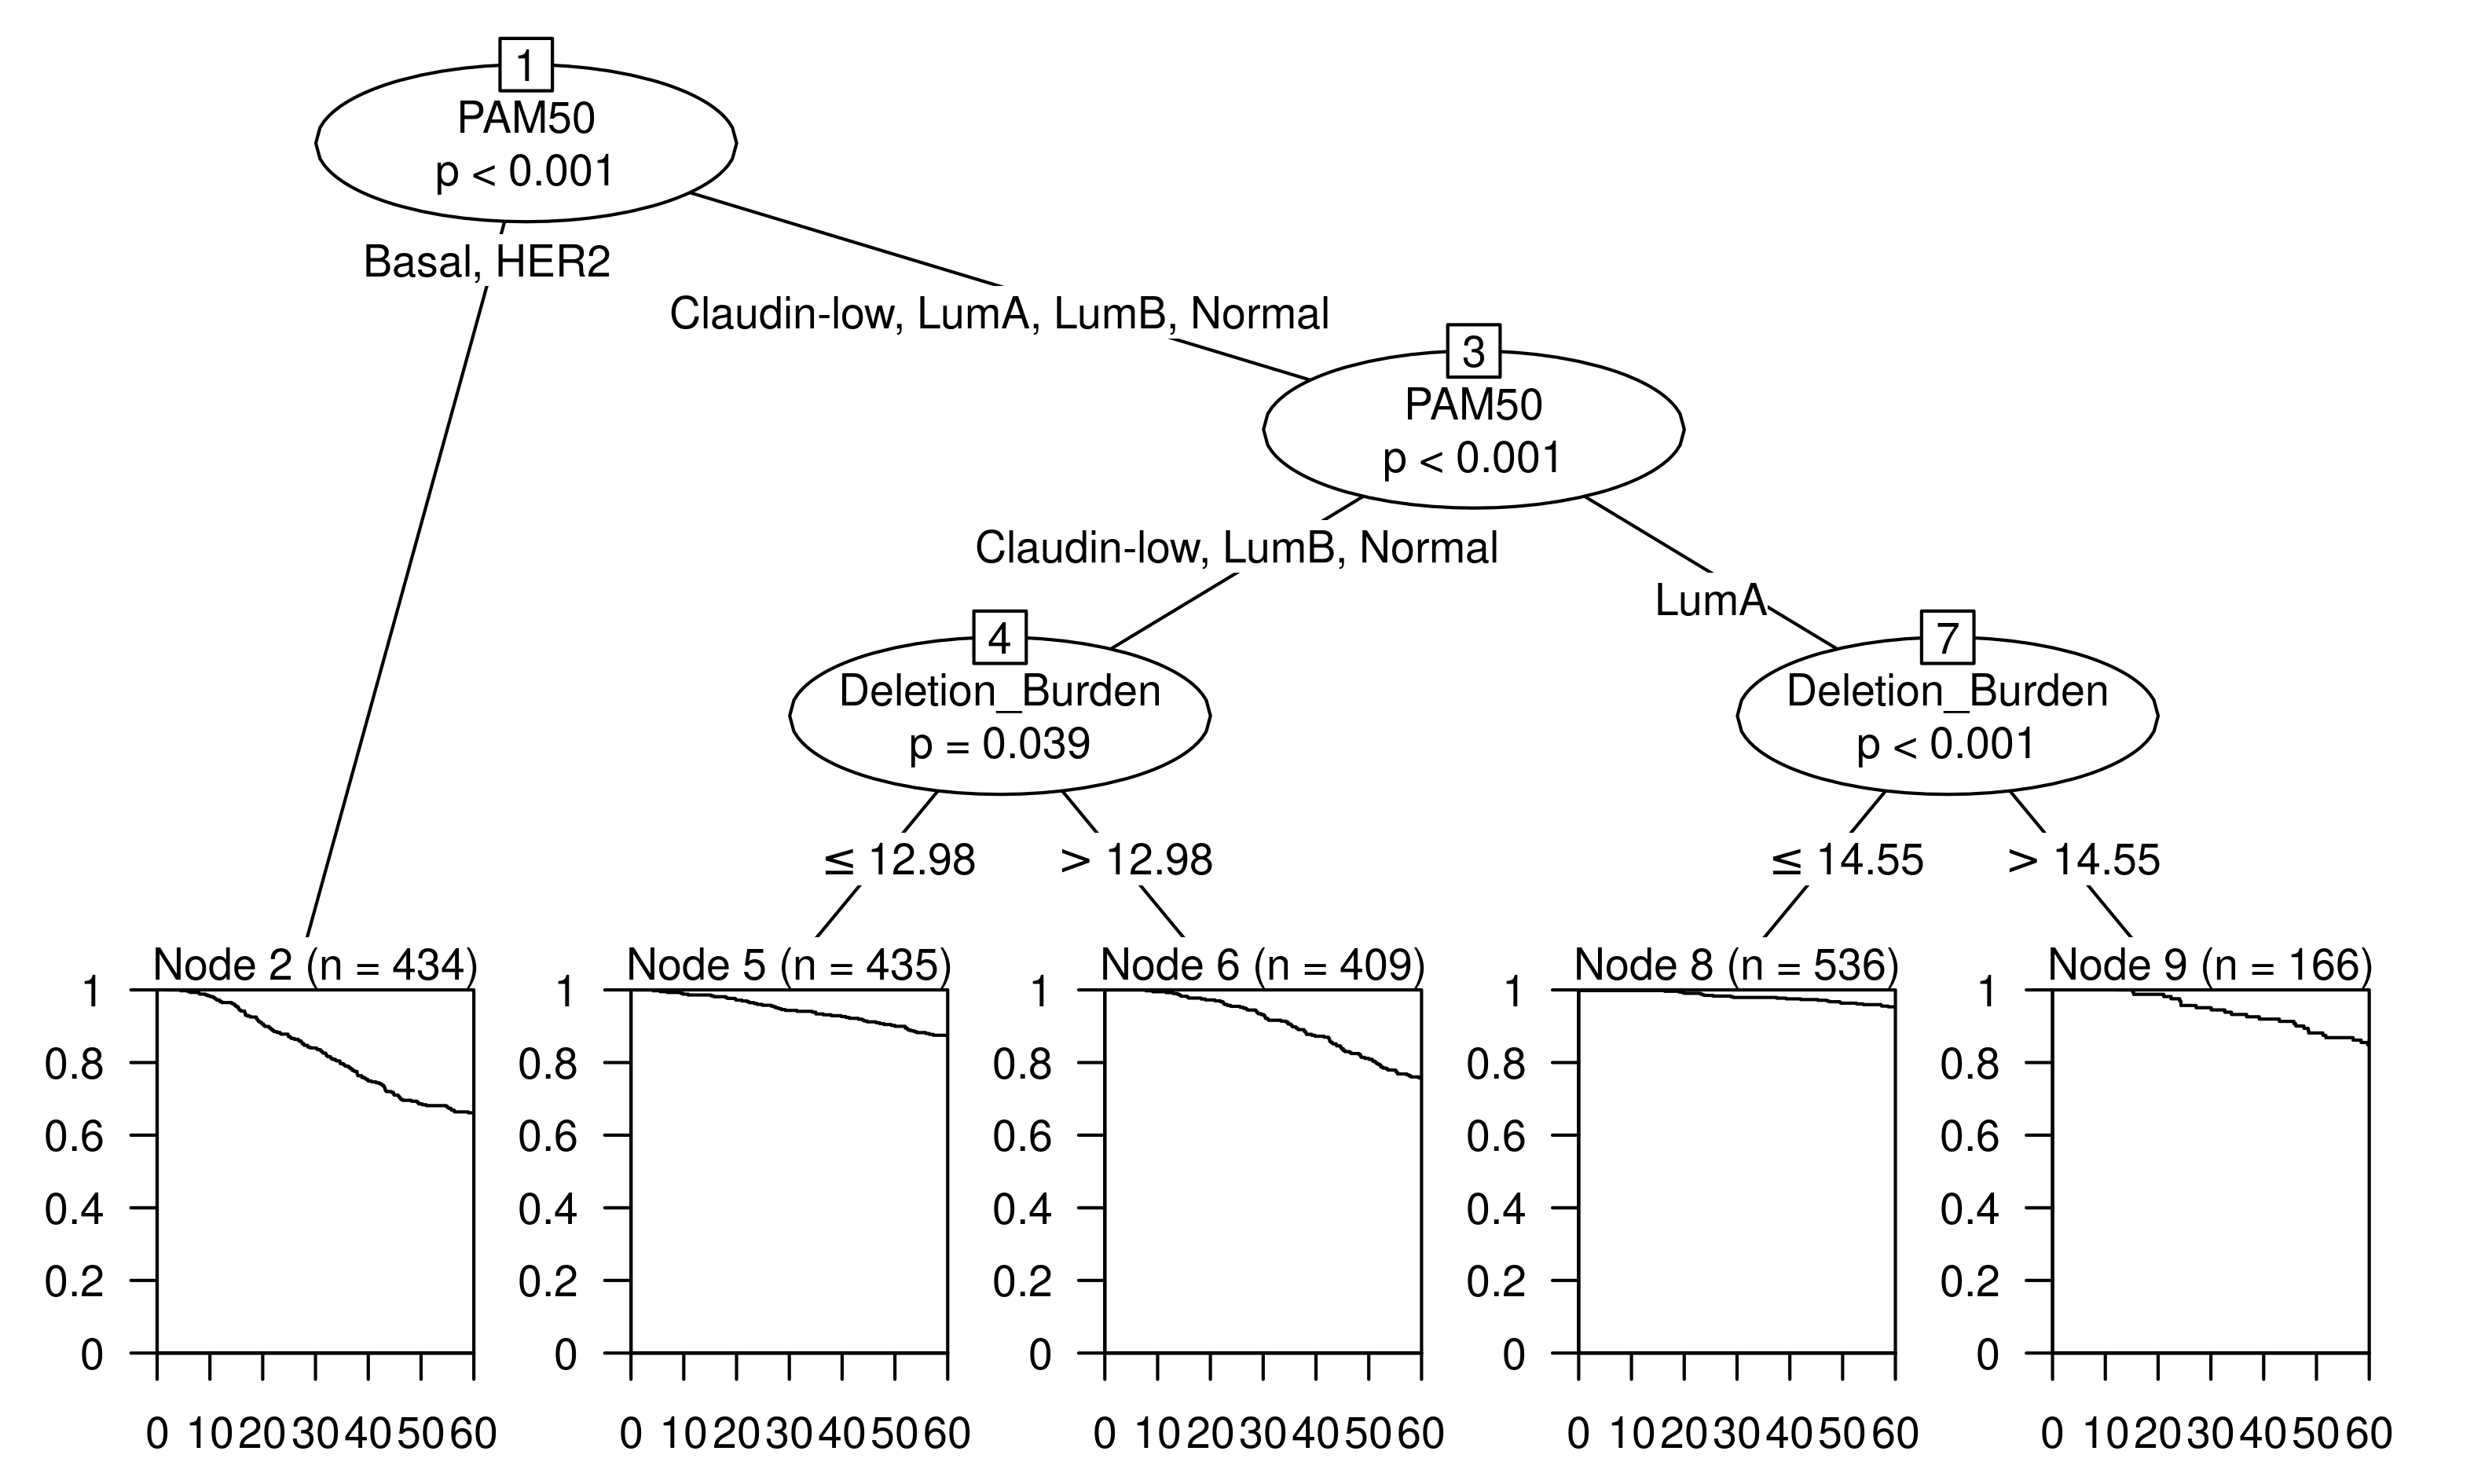
\includegraphics[width=1\textwidth]{../figures/Chapter_3/Ctree_Survival_Burden_FiveYearDSS_PAM50.png}
\end{subfigure}
\vspace{0.5cm}

\caption[Recursive partitioning survival trees for five-year disease-specific survival using PAM50 subtype and the six CNA Burden metrics as candidate predictors.]{Recursive partitioning survival trees for five-year disease-specific survival using PAM50 subtype and the six CNA Burden metrics as candidate predictors. (A) Trees fitted using the rpart algorithm and (B) trees fitted using the ctree algorithm.}
\label{fig:PAM50_CNA_Burden_FiveYearDSS}
\end{figure}

\begin{figure}[!h]
\centering

\vspace{0.5cm}

\begin{subfigure}{\textwidth}
\subcaption{}
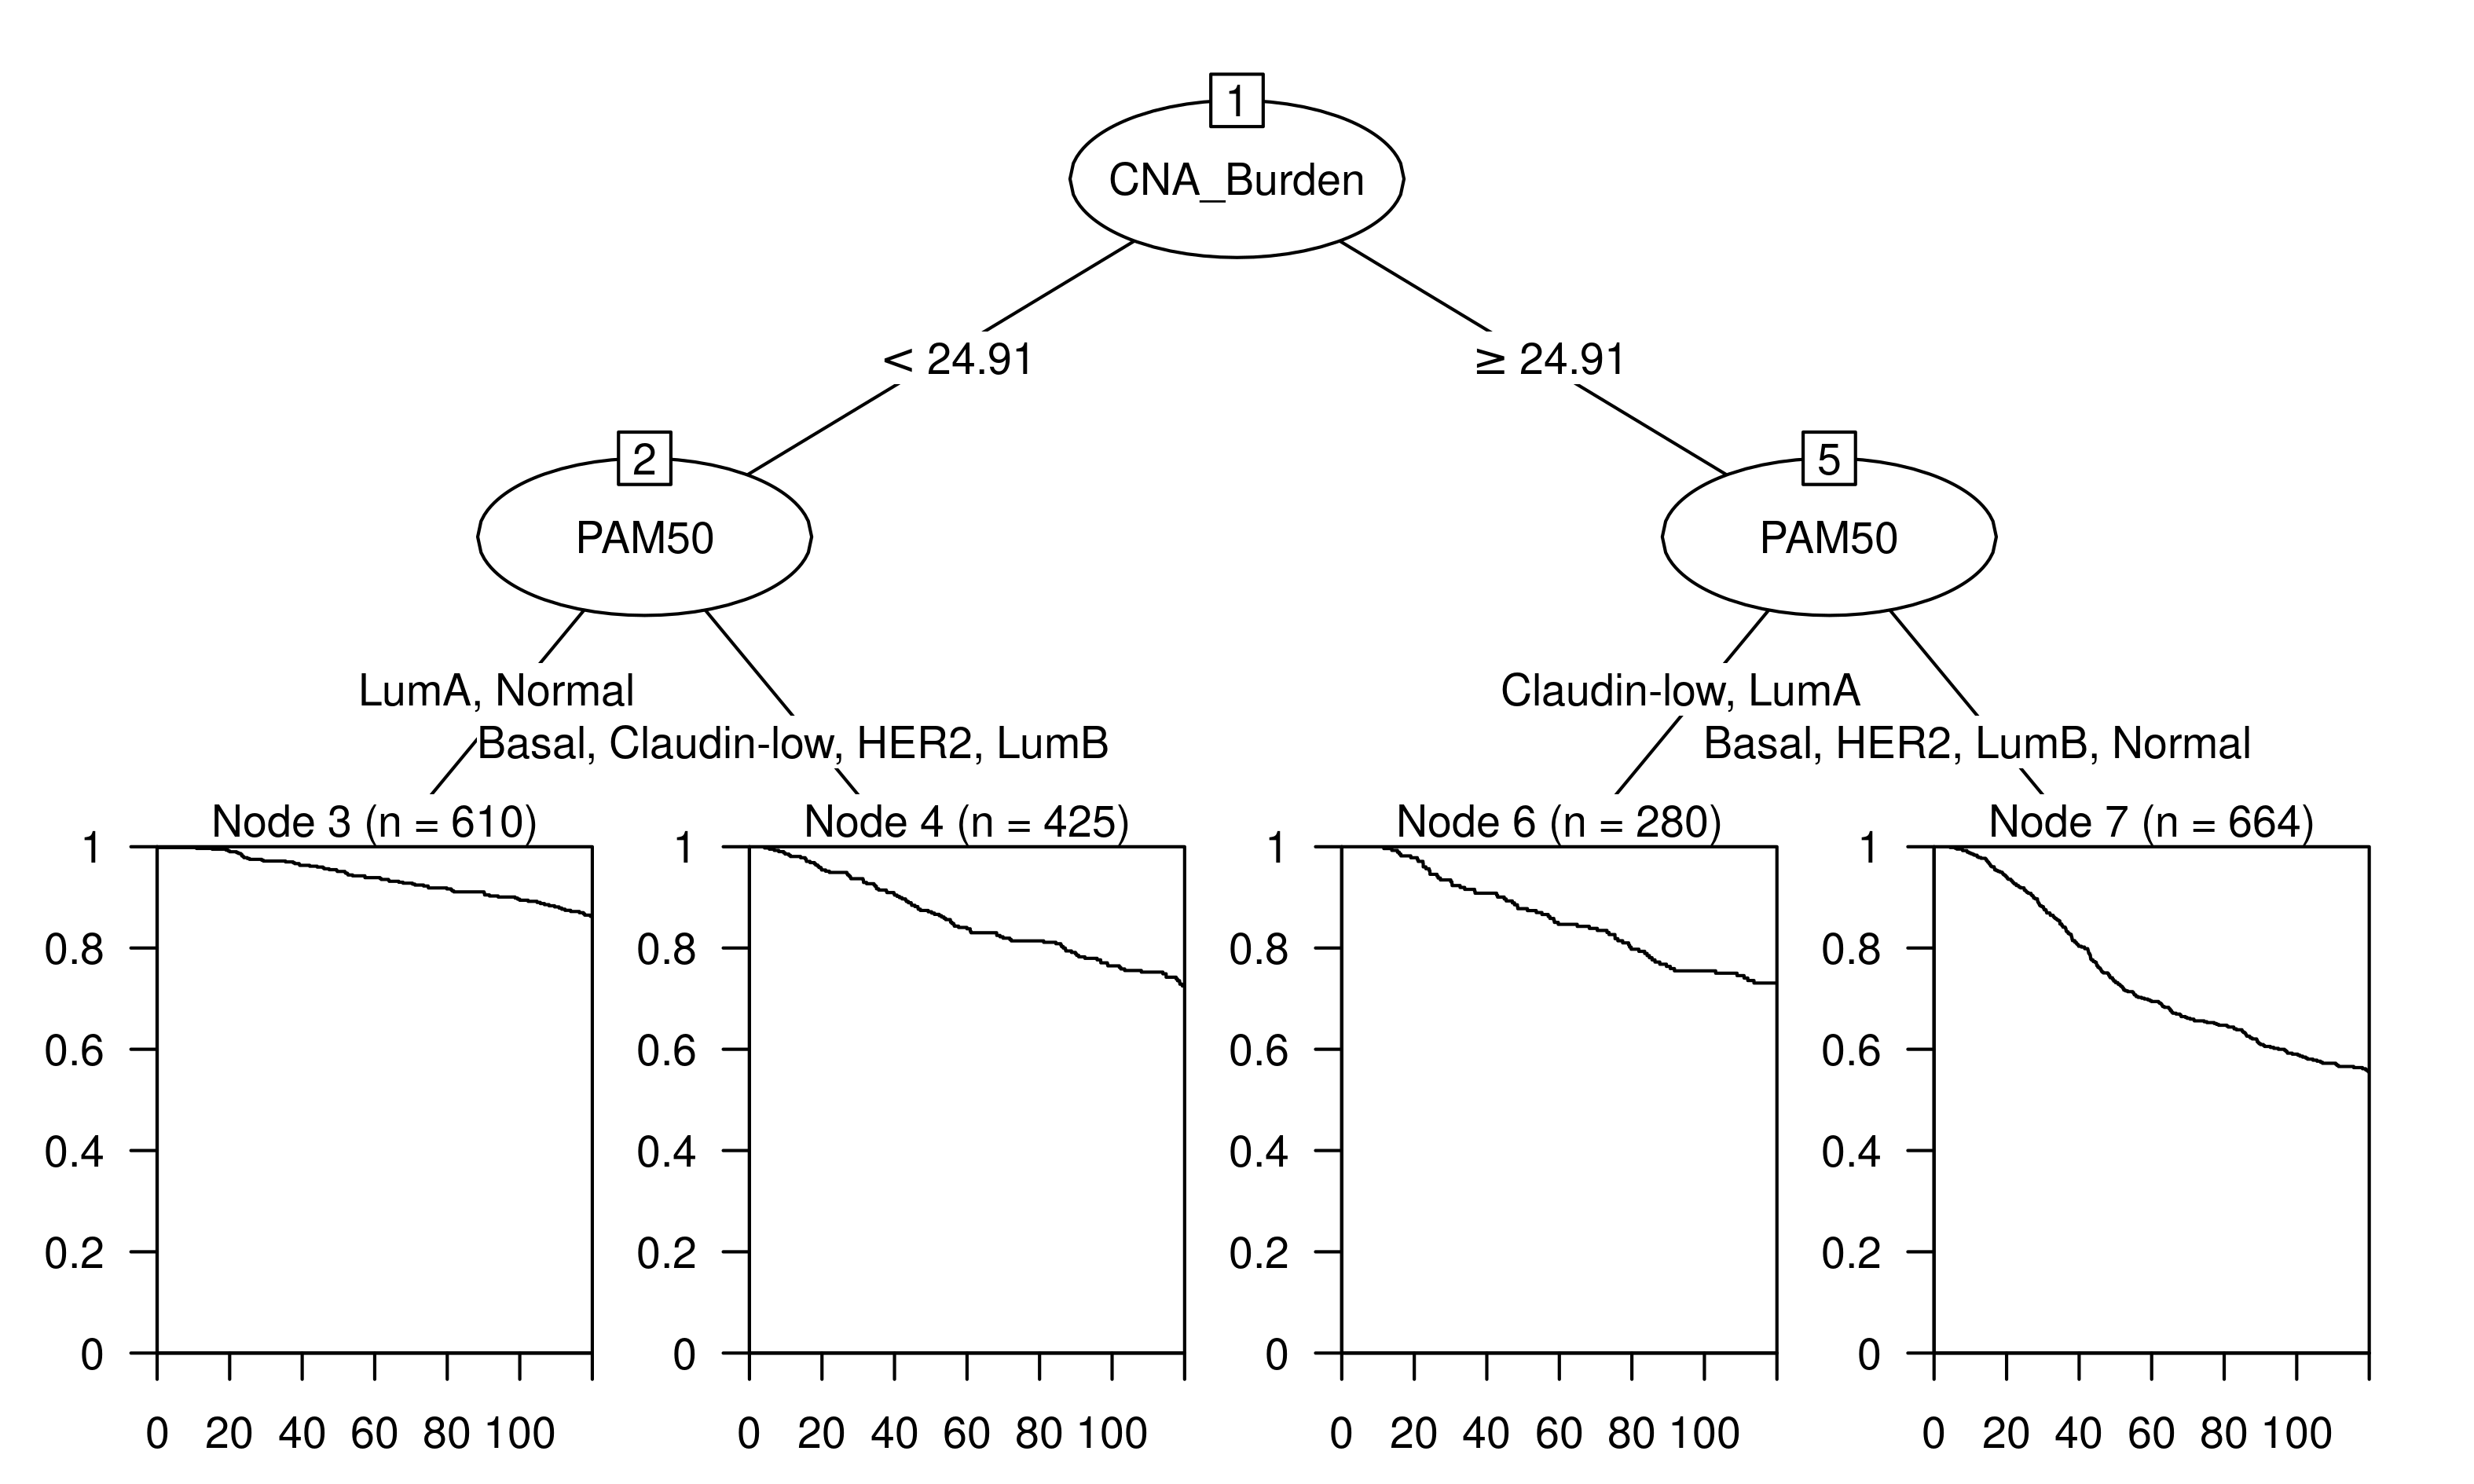
\includegraphics[width=1\textwidth]{../figures/Chapter_3/PartyKit_Survival_Burden_TenYearDSS_PAM50.png}
\end{subfigure}
\vspace{2cm}

\begin{subfigure}{\textwidth}
\subcaption{}
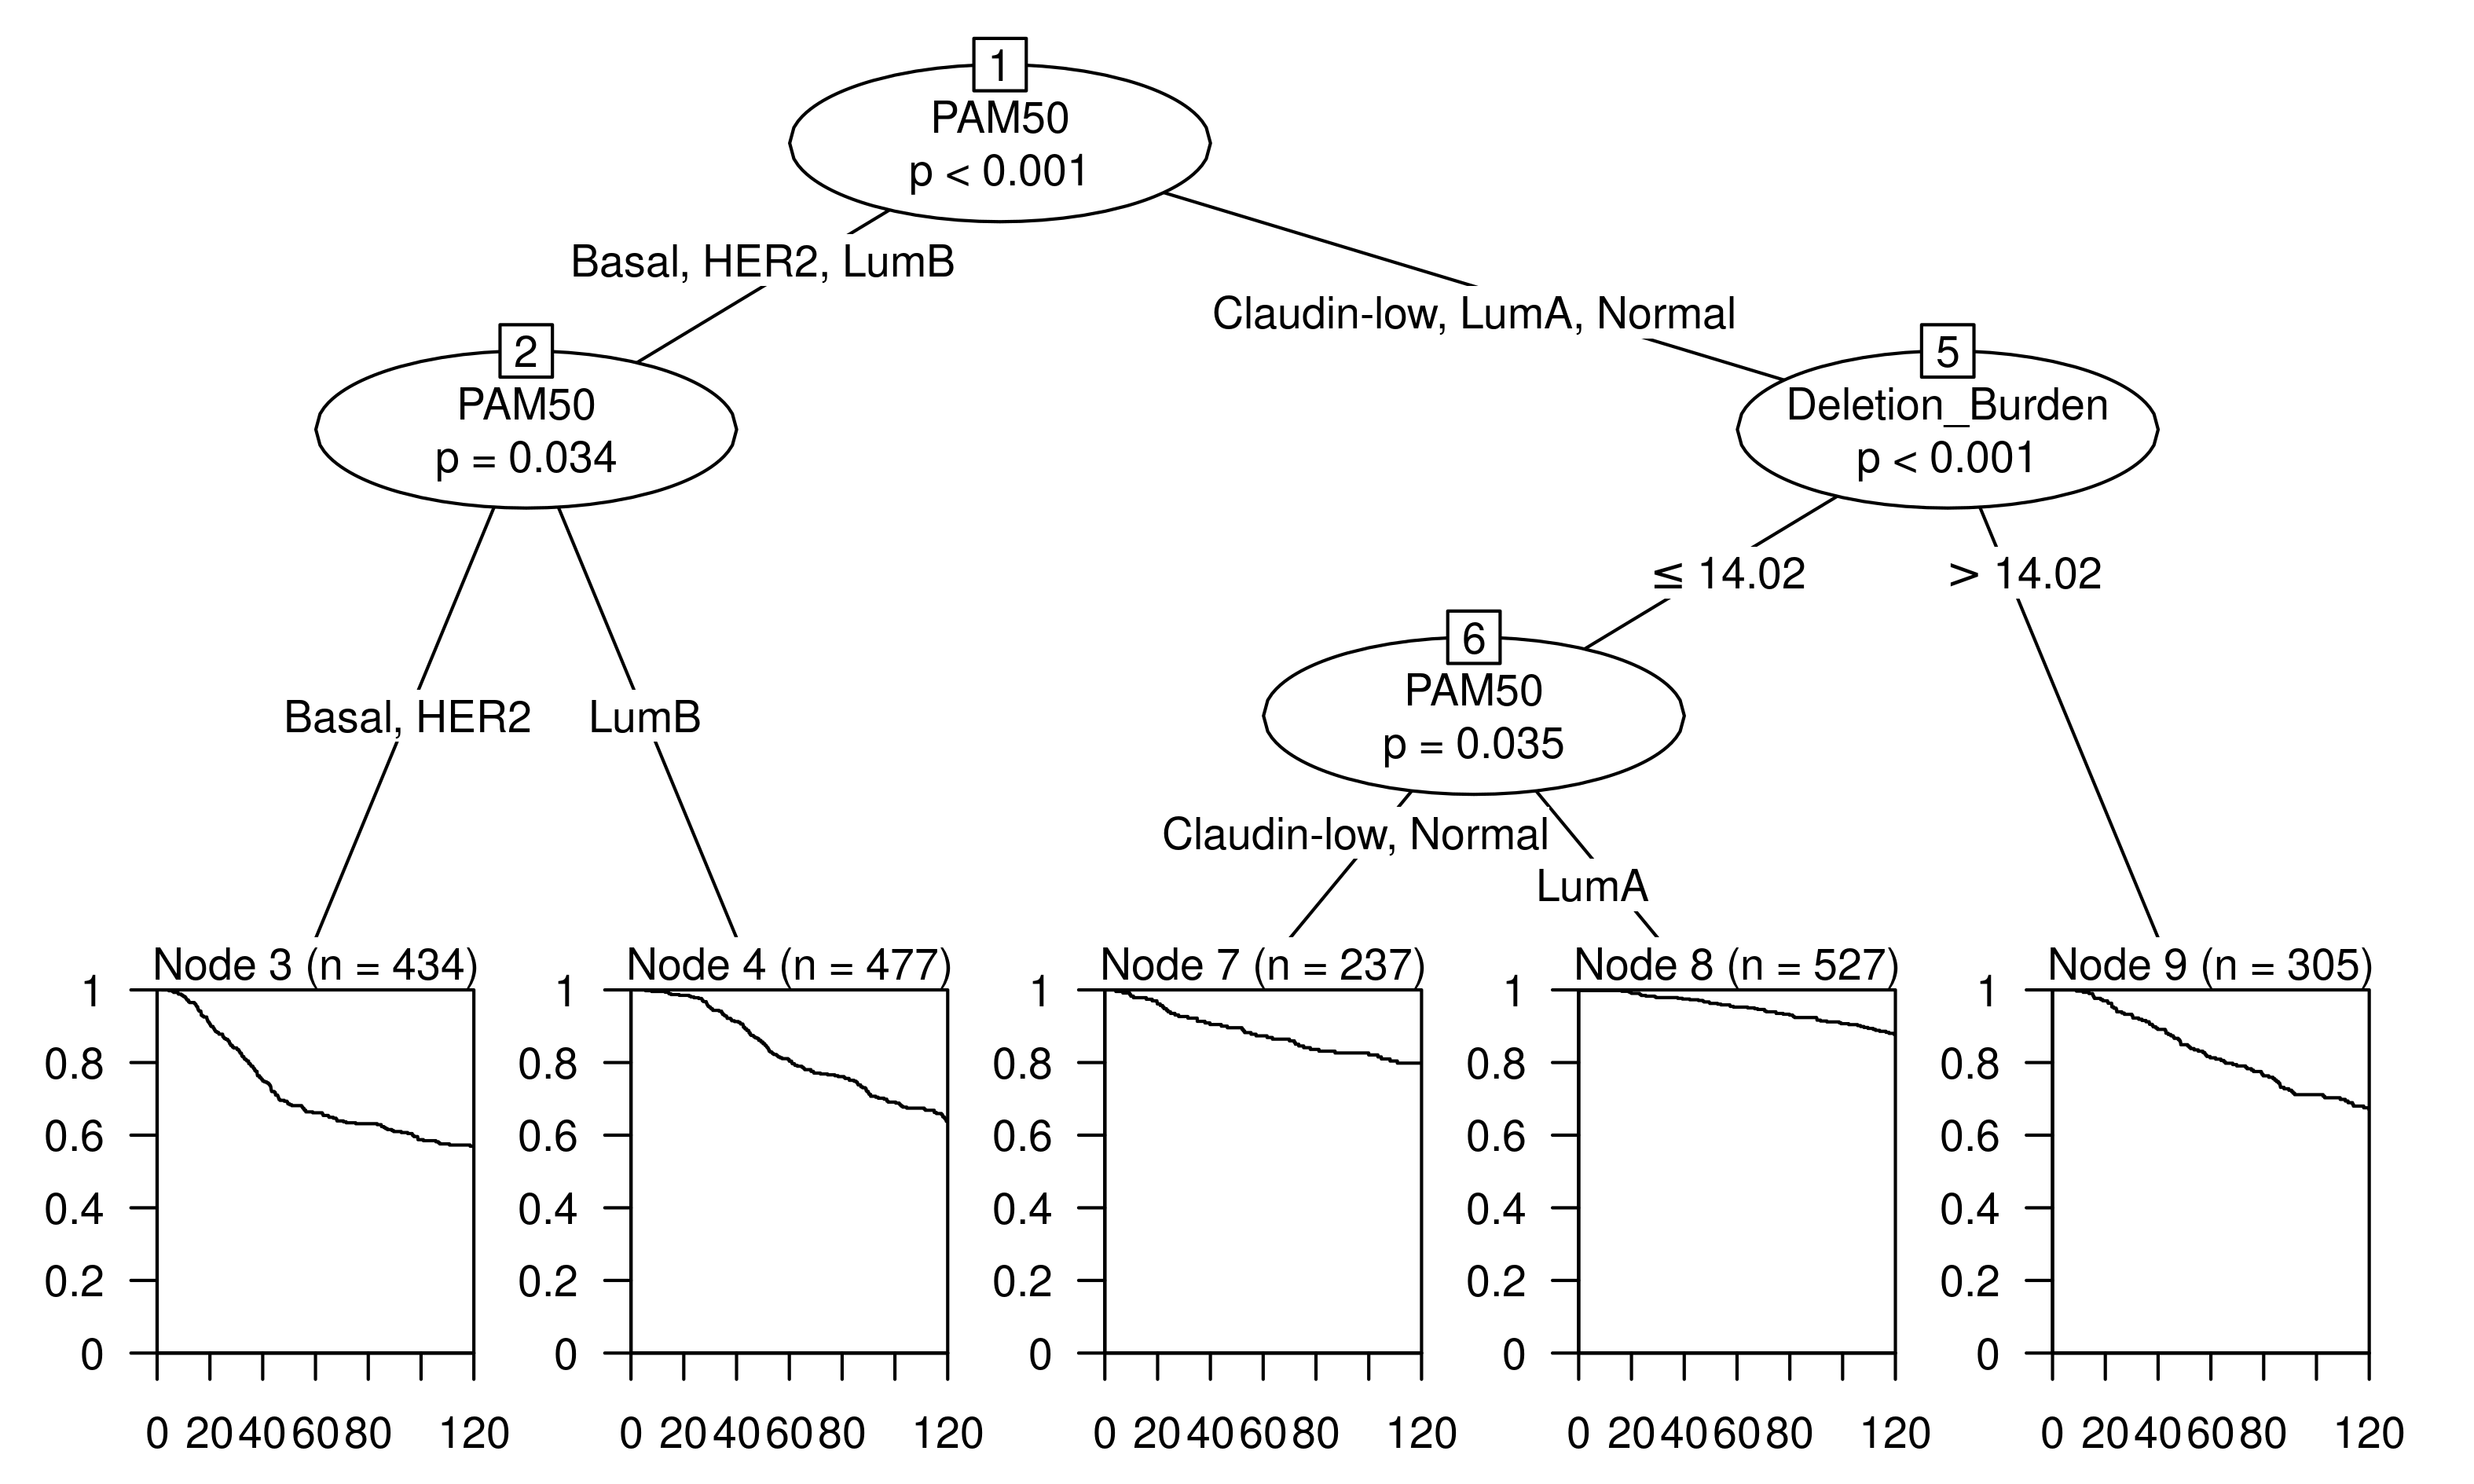
\includegraphics[width=1\textwidth]{../figures/Chapter_3/Ctree_Survival_Burden_TenYearDSS_PAM50.png}
\end{subfigure}
\vspace{0.5cm}

\caption[Recursive partitioning survival trees for ten-year disease-specific survival using PAM50 subtype and the six CNA Burden metrics as candidate predictors.]{Recursive partitioning survival trees for ten-year disease-specific survival using PAM50 subtype and the six CNA Burden metrics as candidate predictors. (A) Trees fitted using the rpart algorithm and (B) trees fitted using the ctree algorithm.}
\label{fig:PAM50_CNA_Burden_TenYearDSS}
\end{figure} 

\begin{figure}[!h]
\centering

\vspace{0.5cm}

\begin{subfigure}{\textwidth}
\subcaption{}
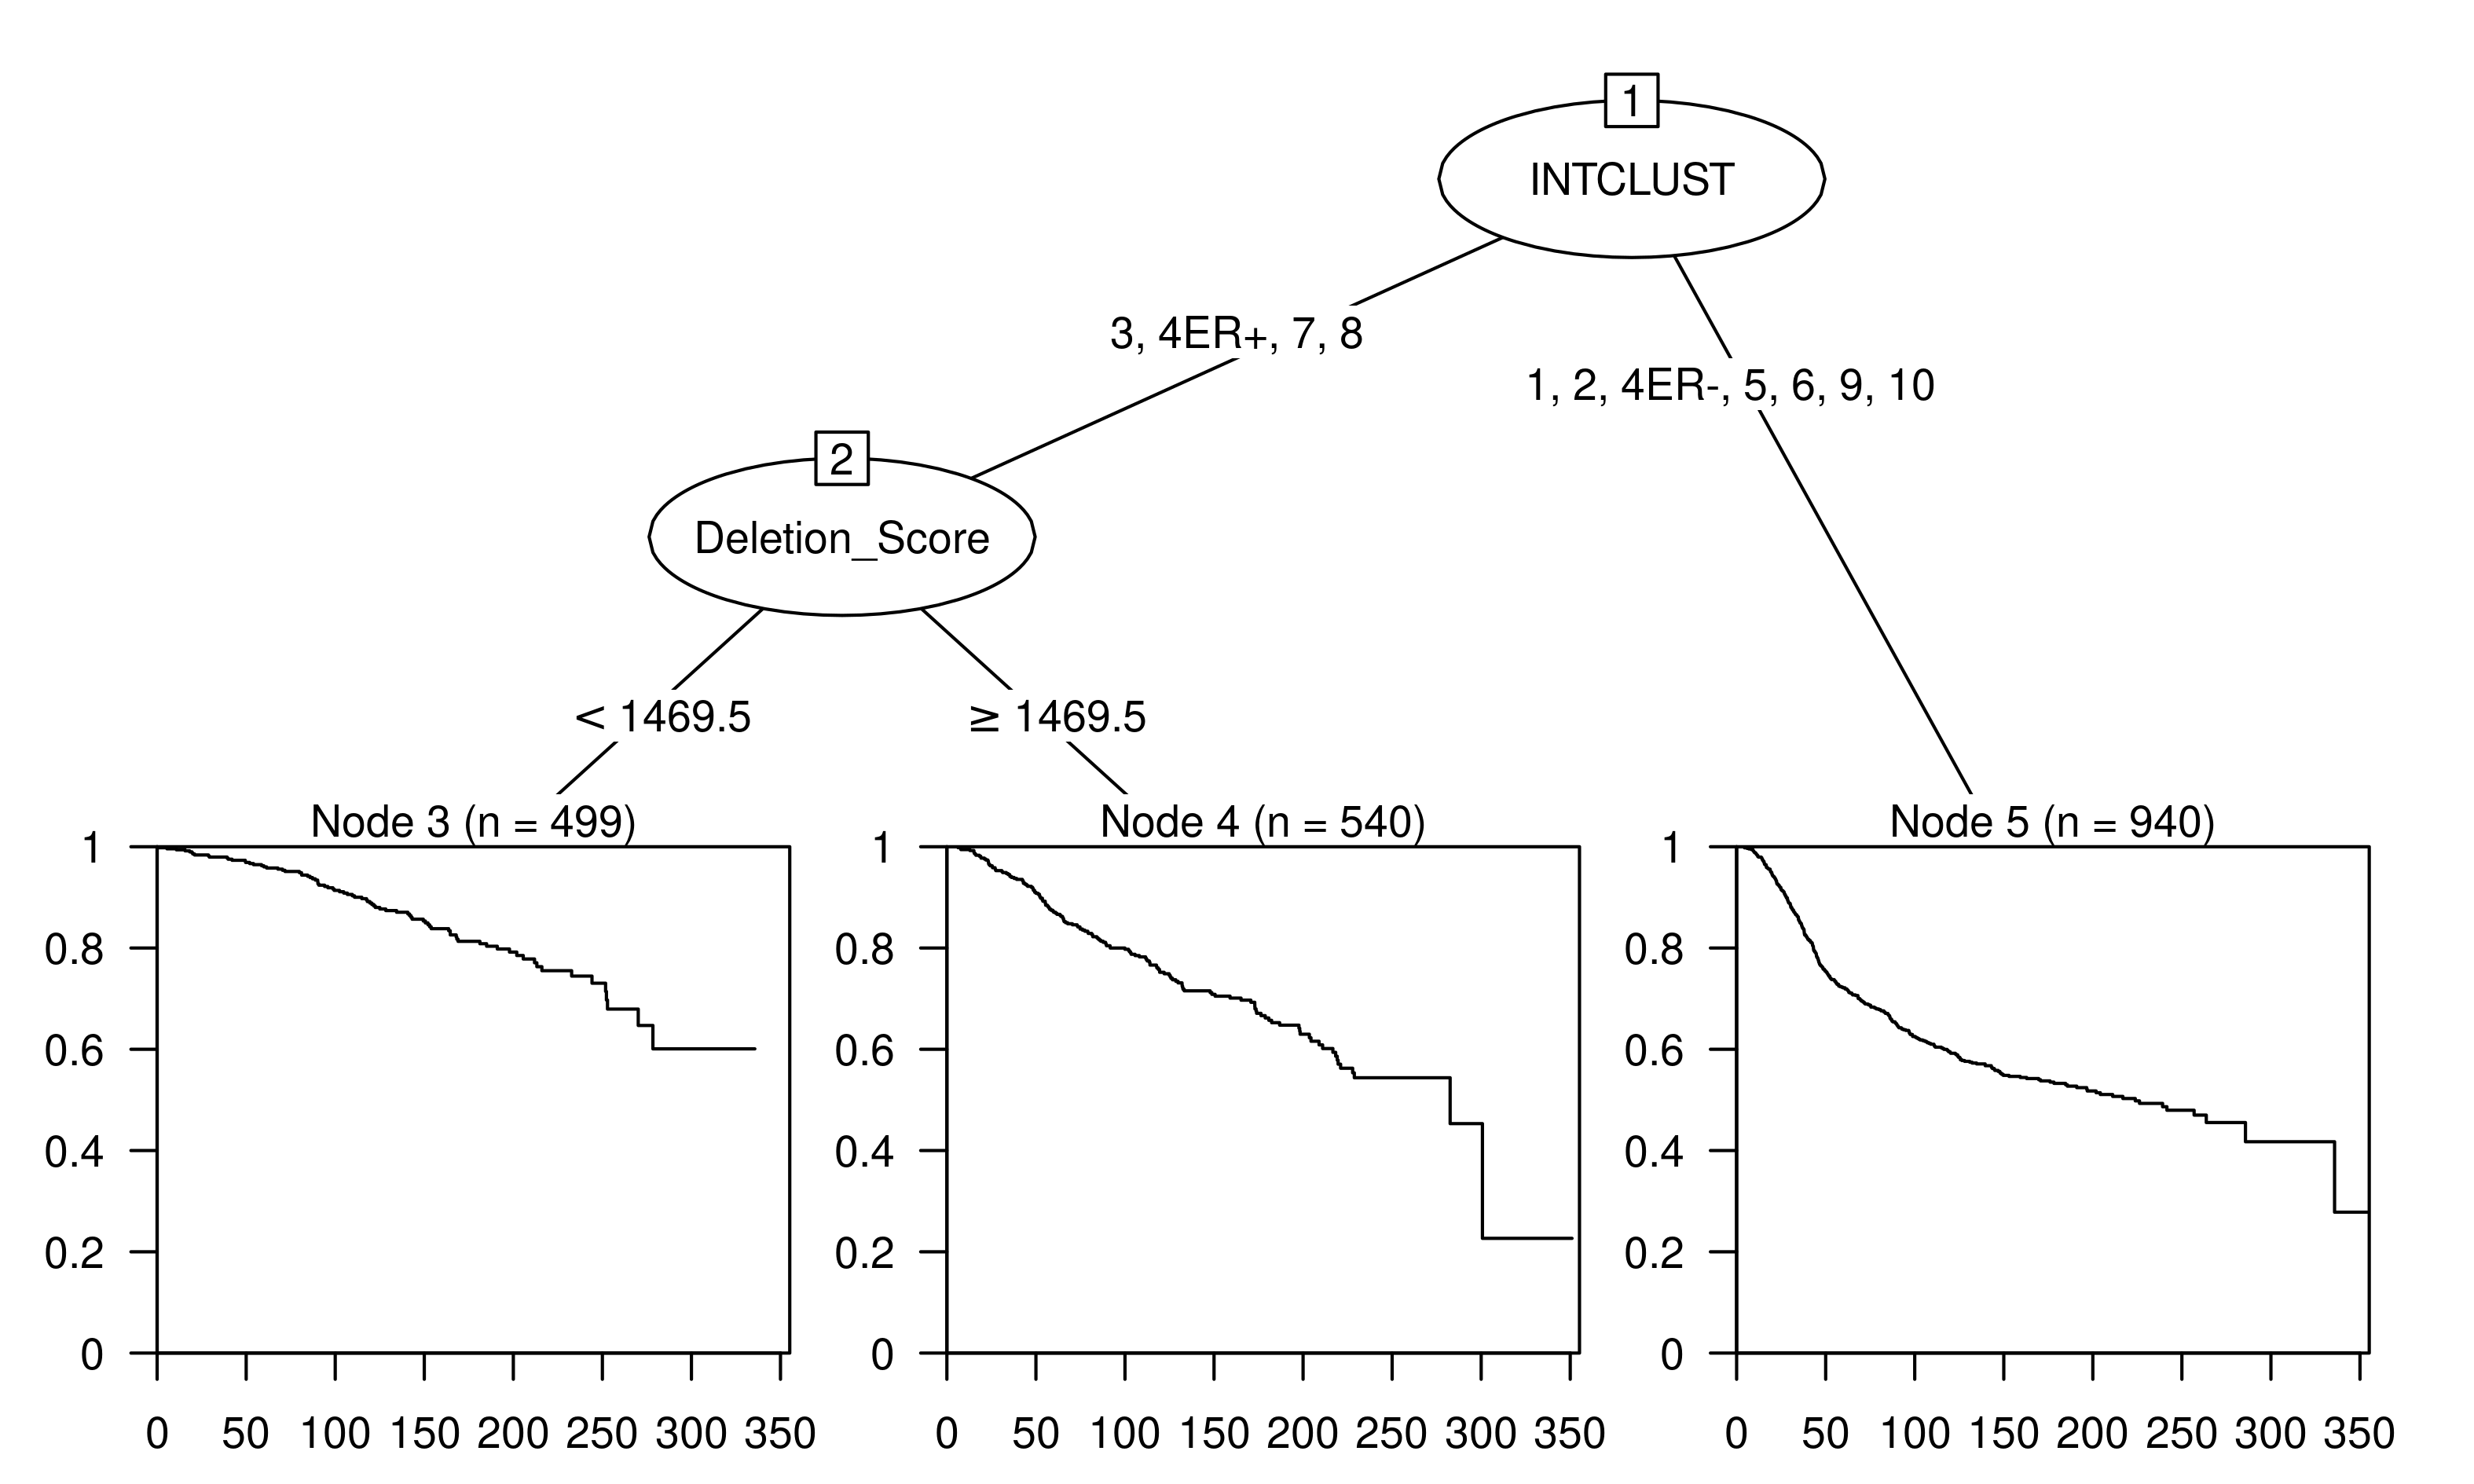
\includegraphics[width=1\textwidth]{../figures/Chapter_3/PartyKit_Survival_Score_DSS_INTCLUST.png}
\end{subfigure}

\vspace{2cm}

\begin{subfigure}{\textwidth}
\subcaption{}
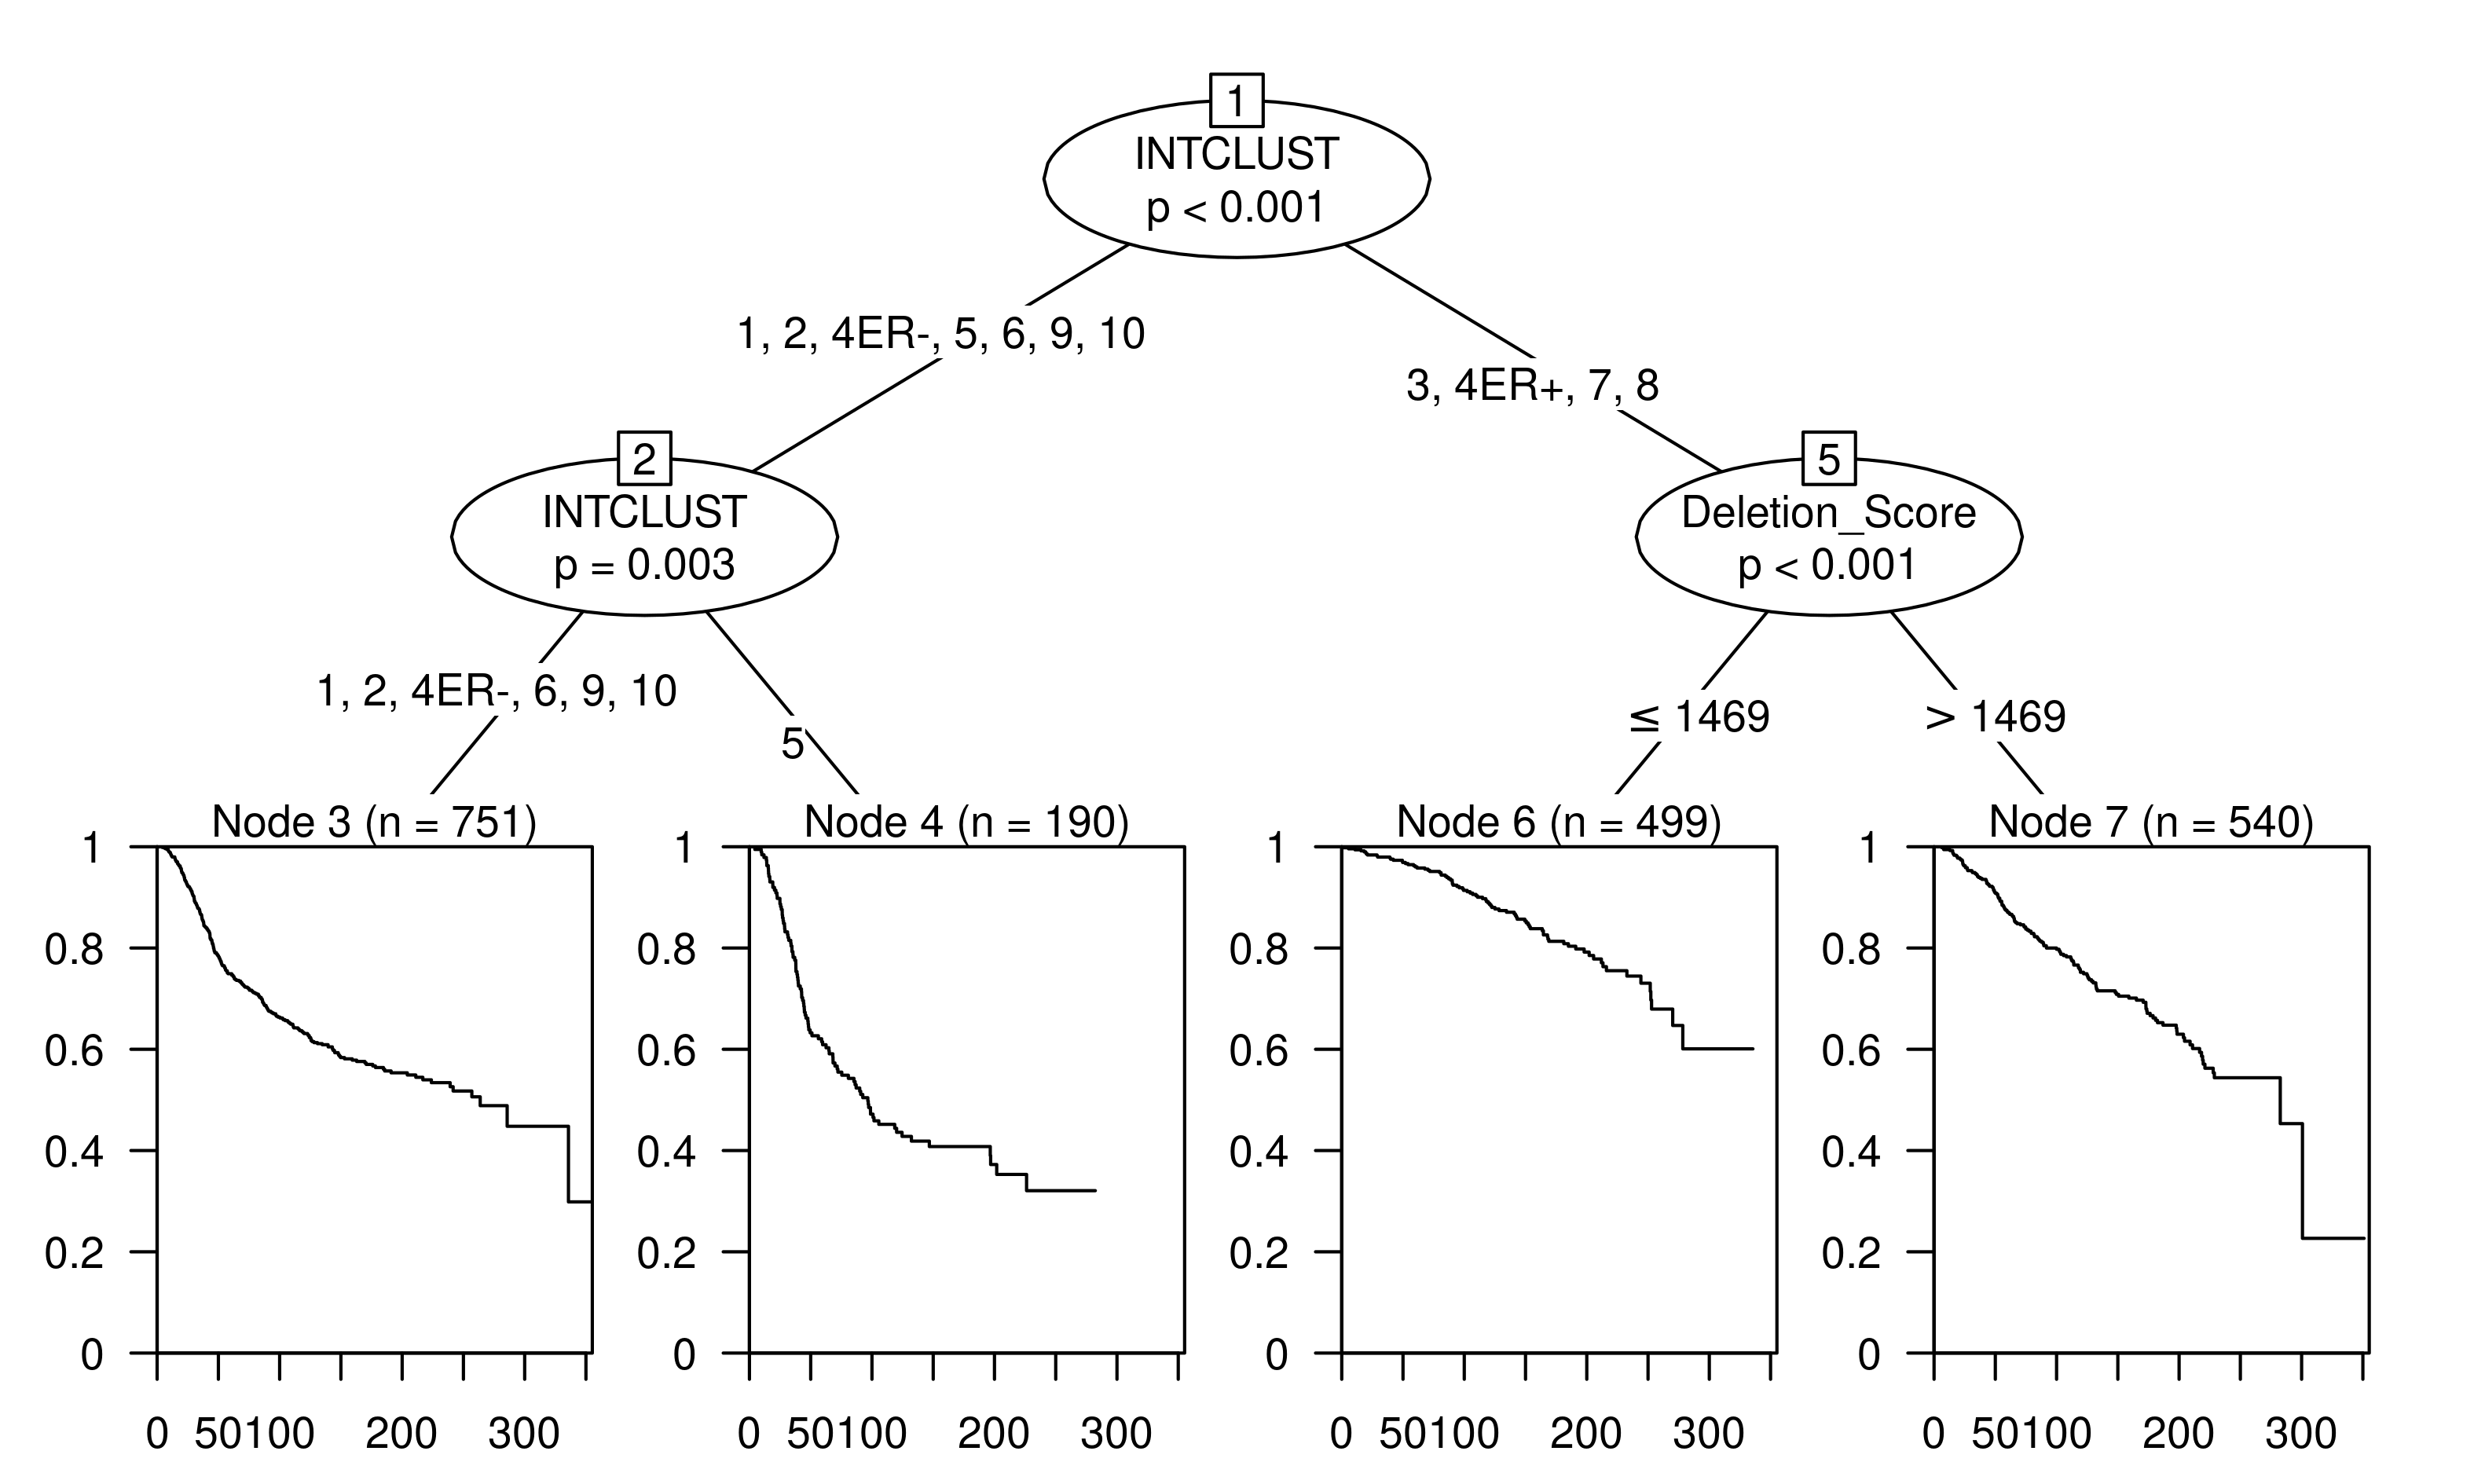
\includegraphics[width=1\textwidth]{../figures/Chapter_3/Ctree_Survival_Score_DSS_INTCLUST.png}
\end{subfigure}

\vspace{0.5cm}

\caption[Recursive partitioning survival trees for disease-specific survival using Integrative Cluster and the six CNA Score metrics as candidate predictors.]{Recursive partitioning survival trees for disease-specific survival using Integrative Cluster and the six CNA Score metrics as candidate predictors. (A) Trees fitted using the rpart algorithm and (B) trees fitted using the ctree algorithm.}
\label{fig:INTCLUST_CNA_Score_DSS}
\end{figure}

\begin{figure}[!h]
\centering

\vspace{0.5cm}

\begin{subfigure}{\textwidth}
\subcaption{}
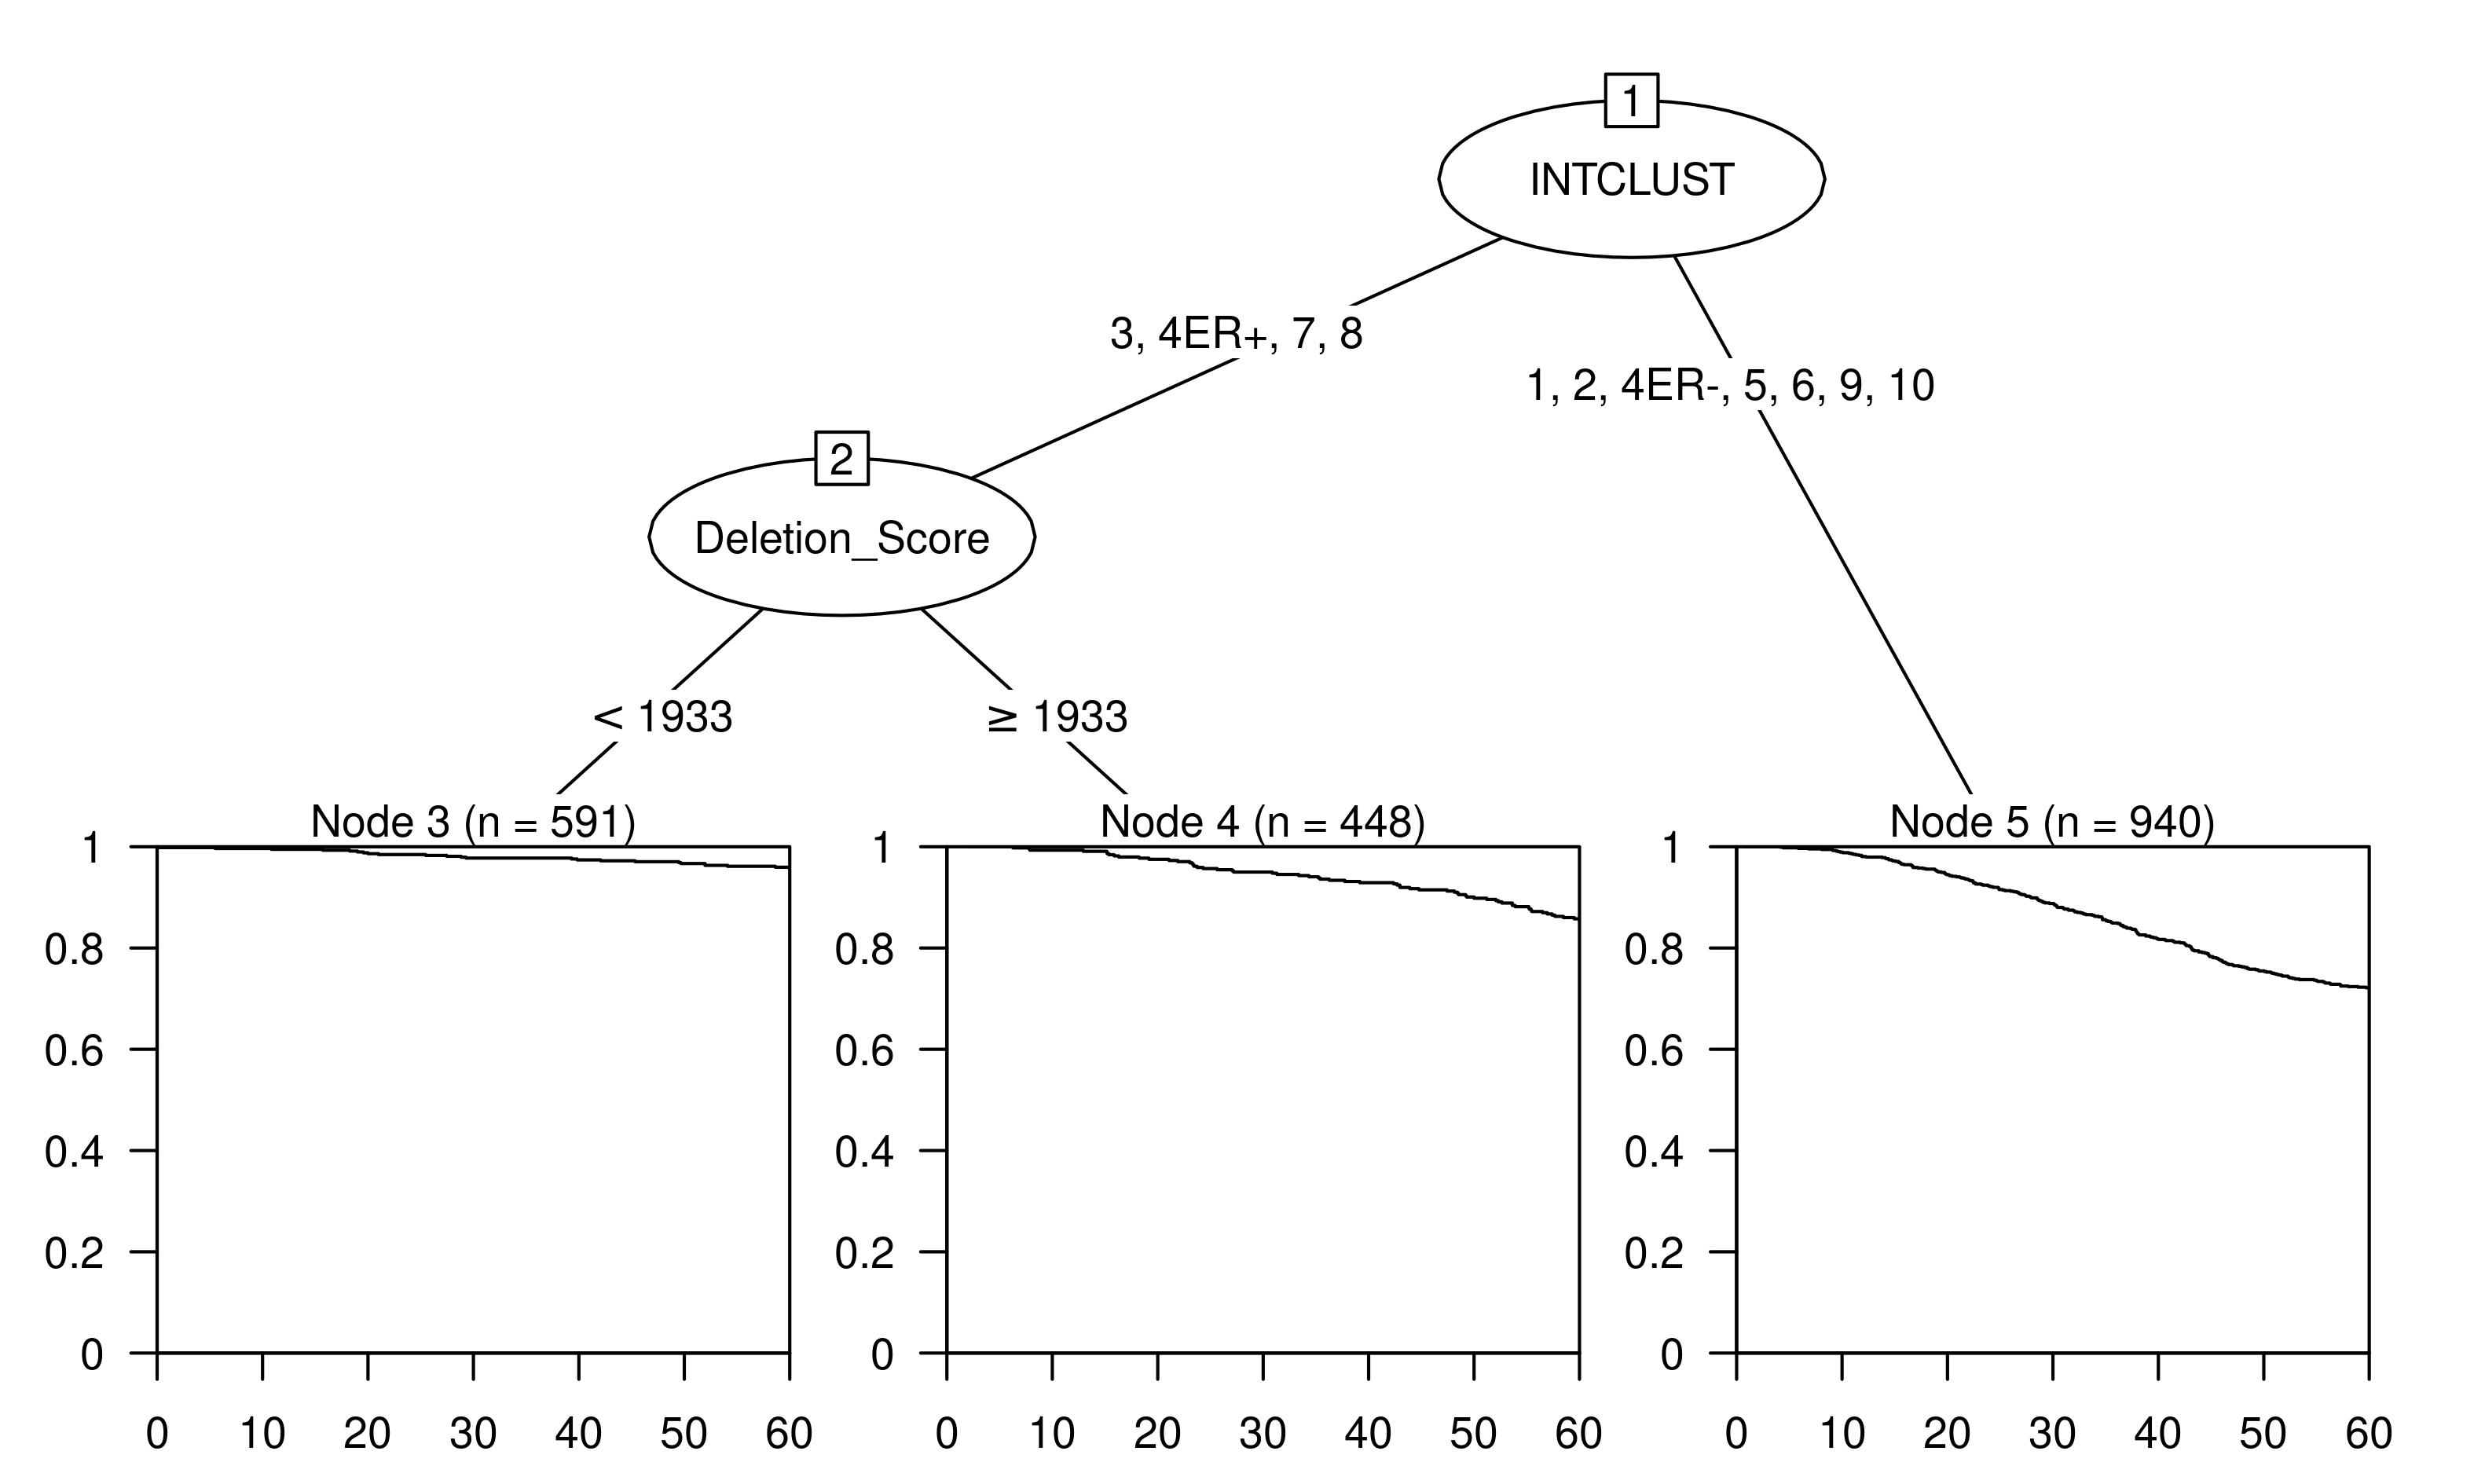
\includegraphics[width=1\textwidth]{../figures/Chapter_3/PartyKit_Survival_Score_FiveYearDSS_INTCLUST.png}
\end{subfigure}

\vspace{2cm}

\begin{subfigure}{\textwidth}
\subcaption{}
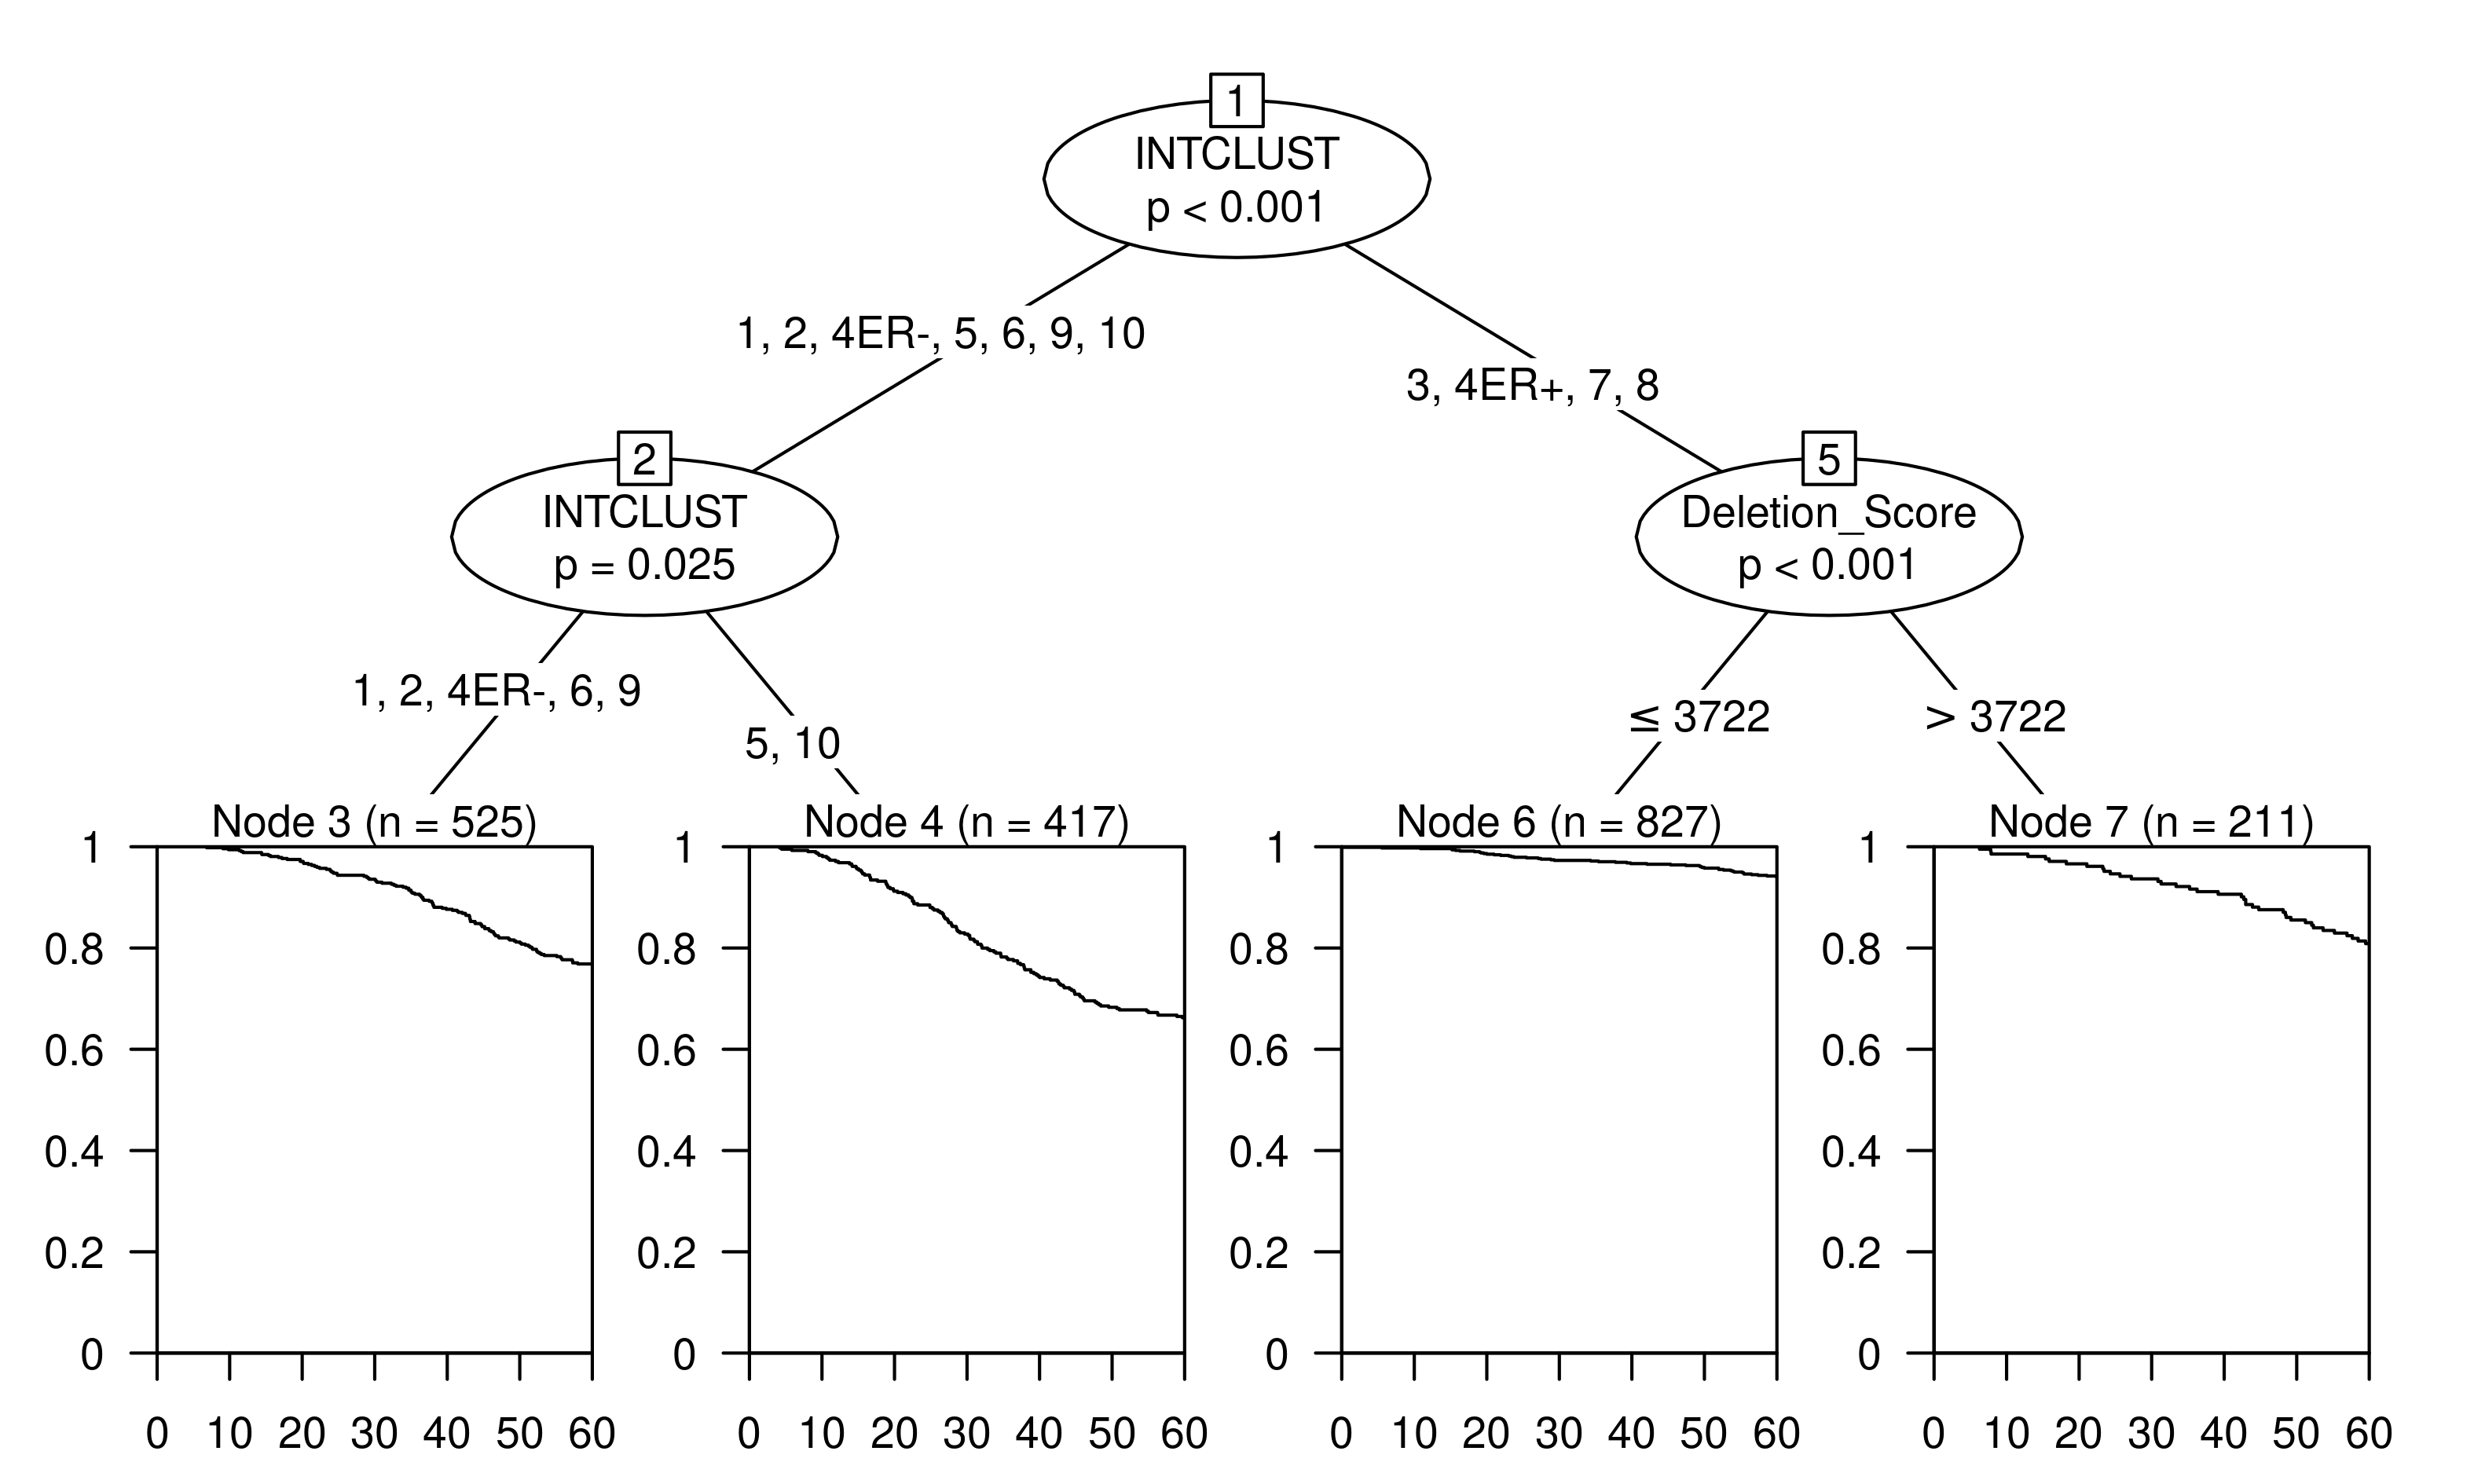
\includegraphics[width=1\textwidth]{../figures/Chapter_3/Ctree_Survival_Score_FiveYearDSS_INTCLUST.png}
\end{subfigure}

\vspace{0.5cm}

\caption[Recursive partitioning survival trees for five-year disease-specific survival using Integrative Cluster and the six CNA Score metrics as candidate predictors.]{Recursive partitioning survival trees for five-year disease-specific survival using Integrative Cluster and the six CNA Score metrics as candidate predictors. (A) Trees fitted using the rpart algorithm and (B) trees fitted using the ctree algorithm.}
\label{fig:INTCLUST_CNA_Score_FiveYearDSS}
\end{figure}

\begin{figure}[!h]
\centering

\vspace{0.5cm}

\begin{subfigure}{\textwidth}
\subcaption{}
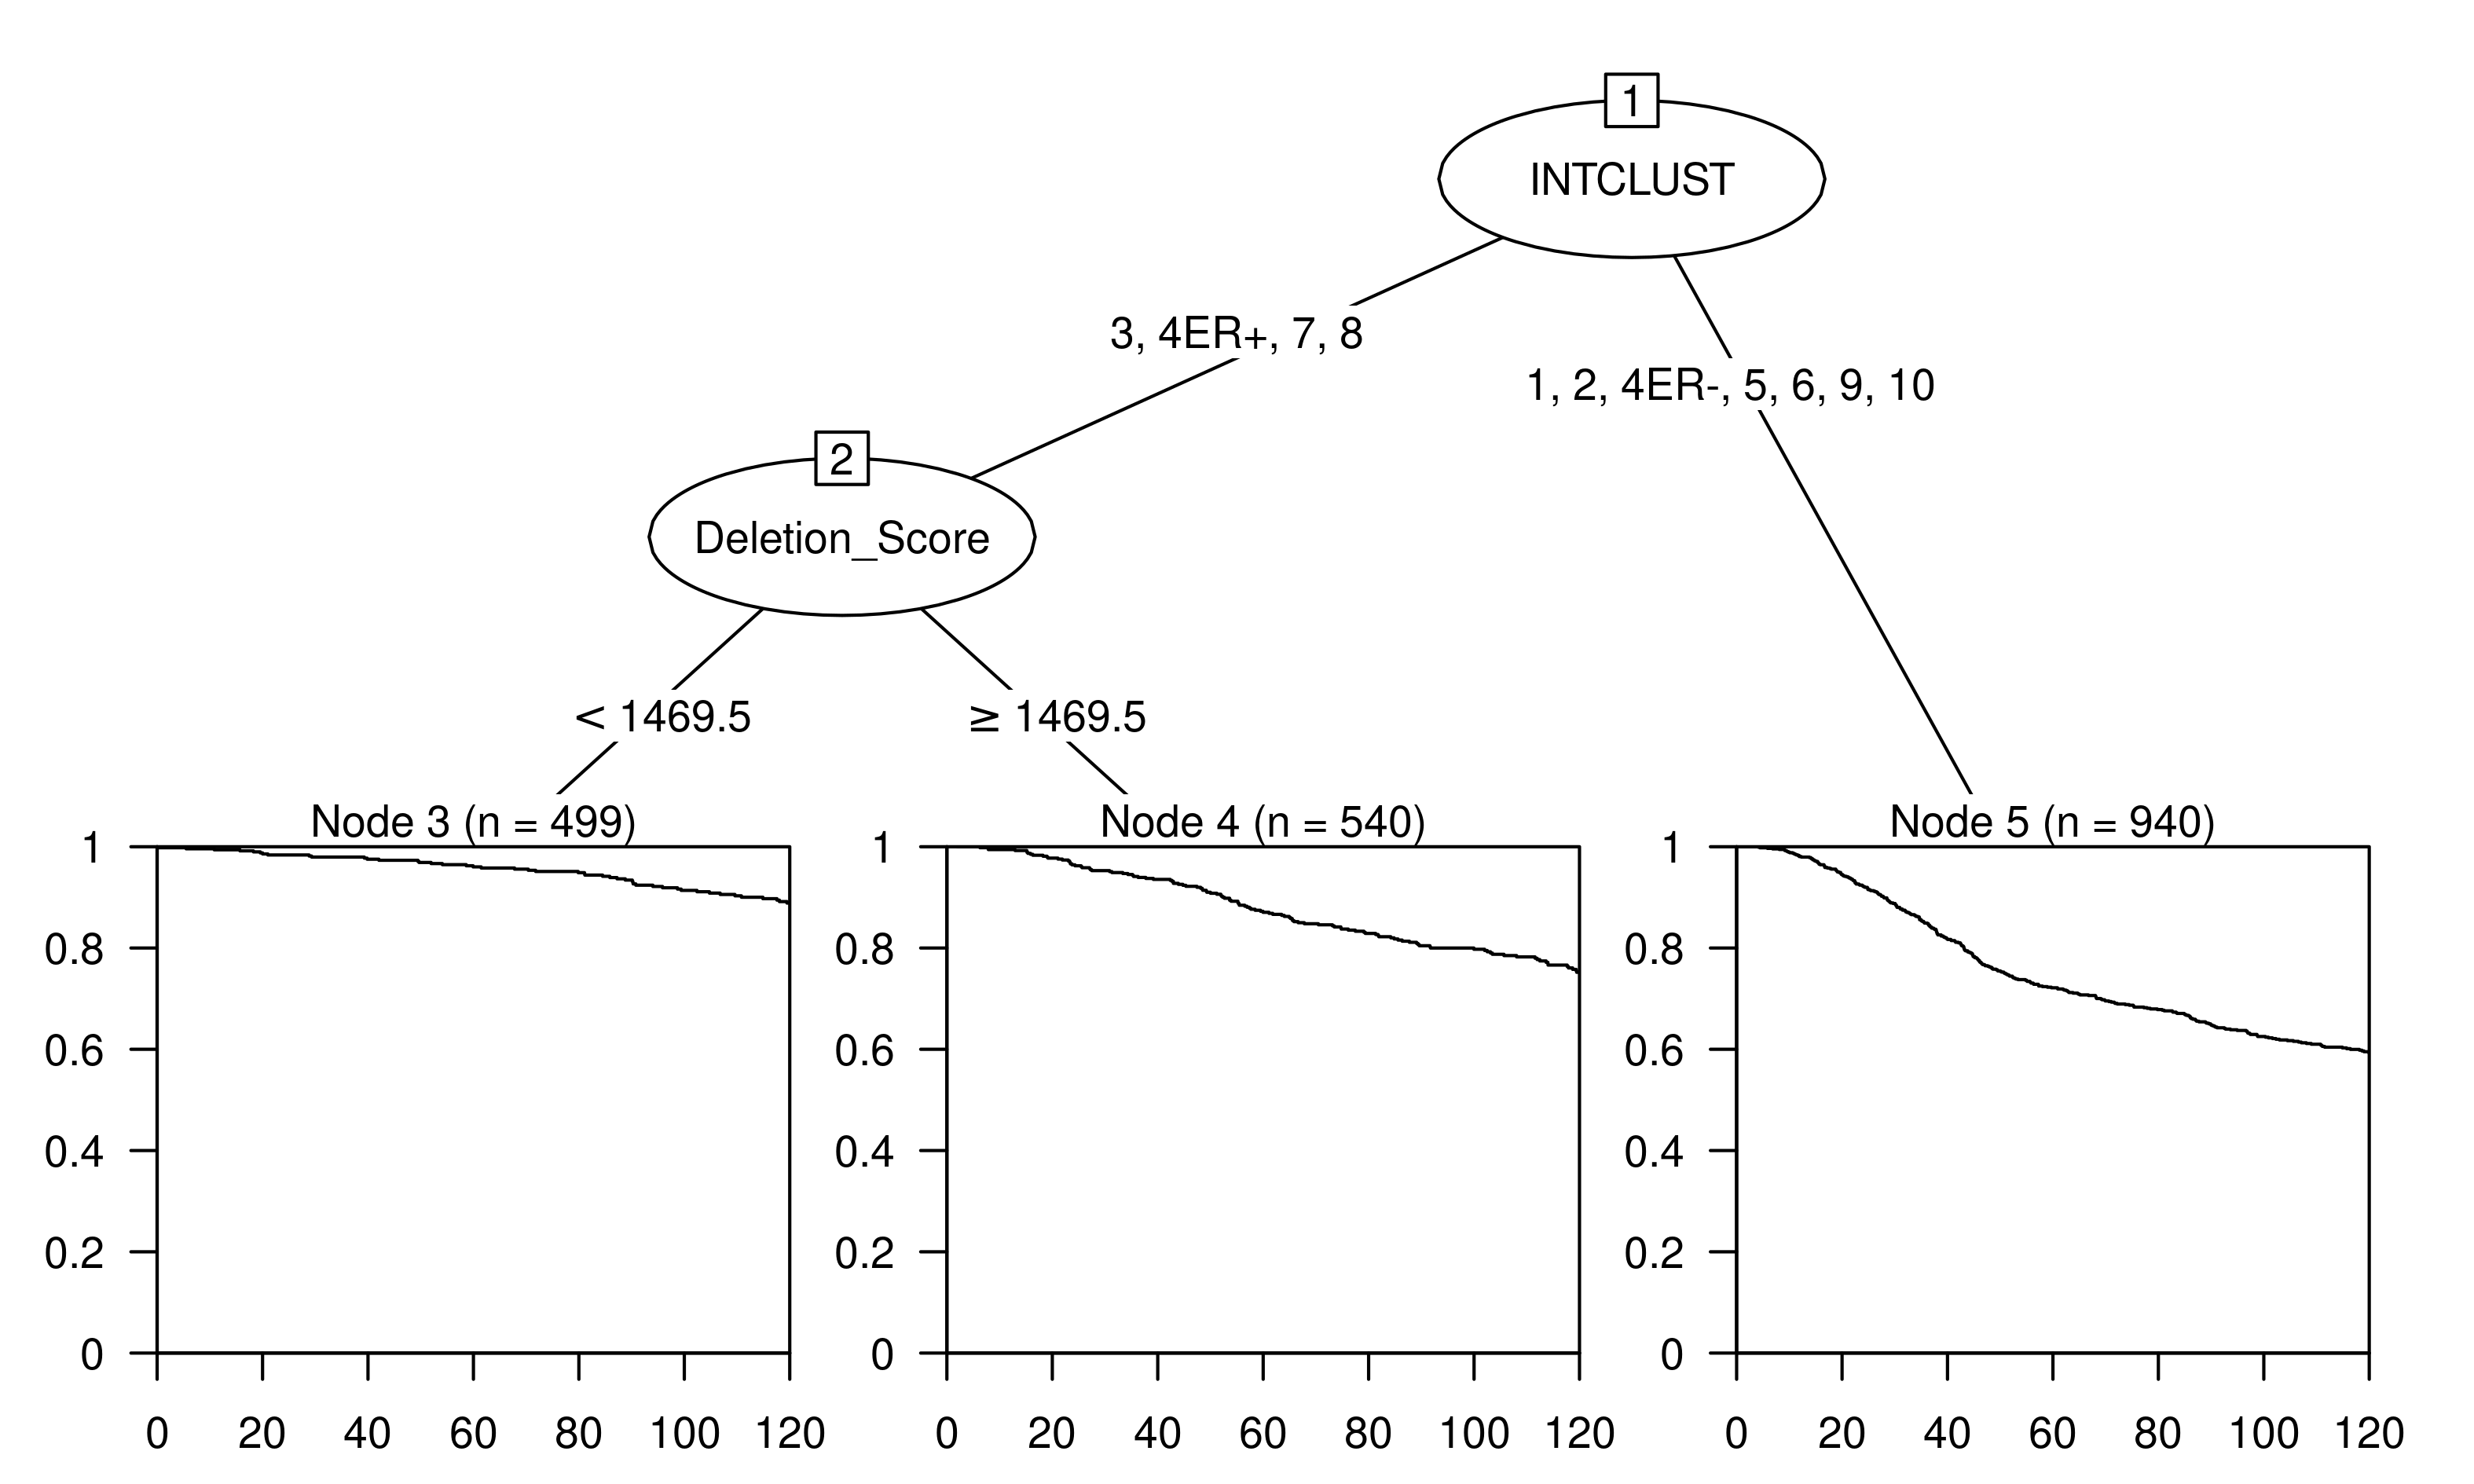
\includegraphics[width=1\textwidth]{../figures/Chapter_3/PartyKit_Survival_Score_TenYearDSS_INTCLUST.png}
\end{subfigure}

\vspace{2cm}

\begin{subfigure}{\textwidth}
\subcaption{}
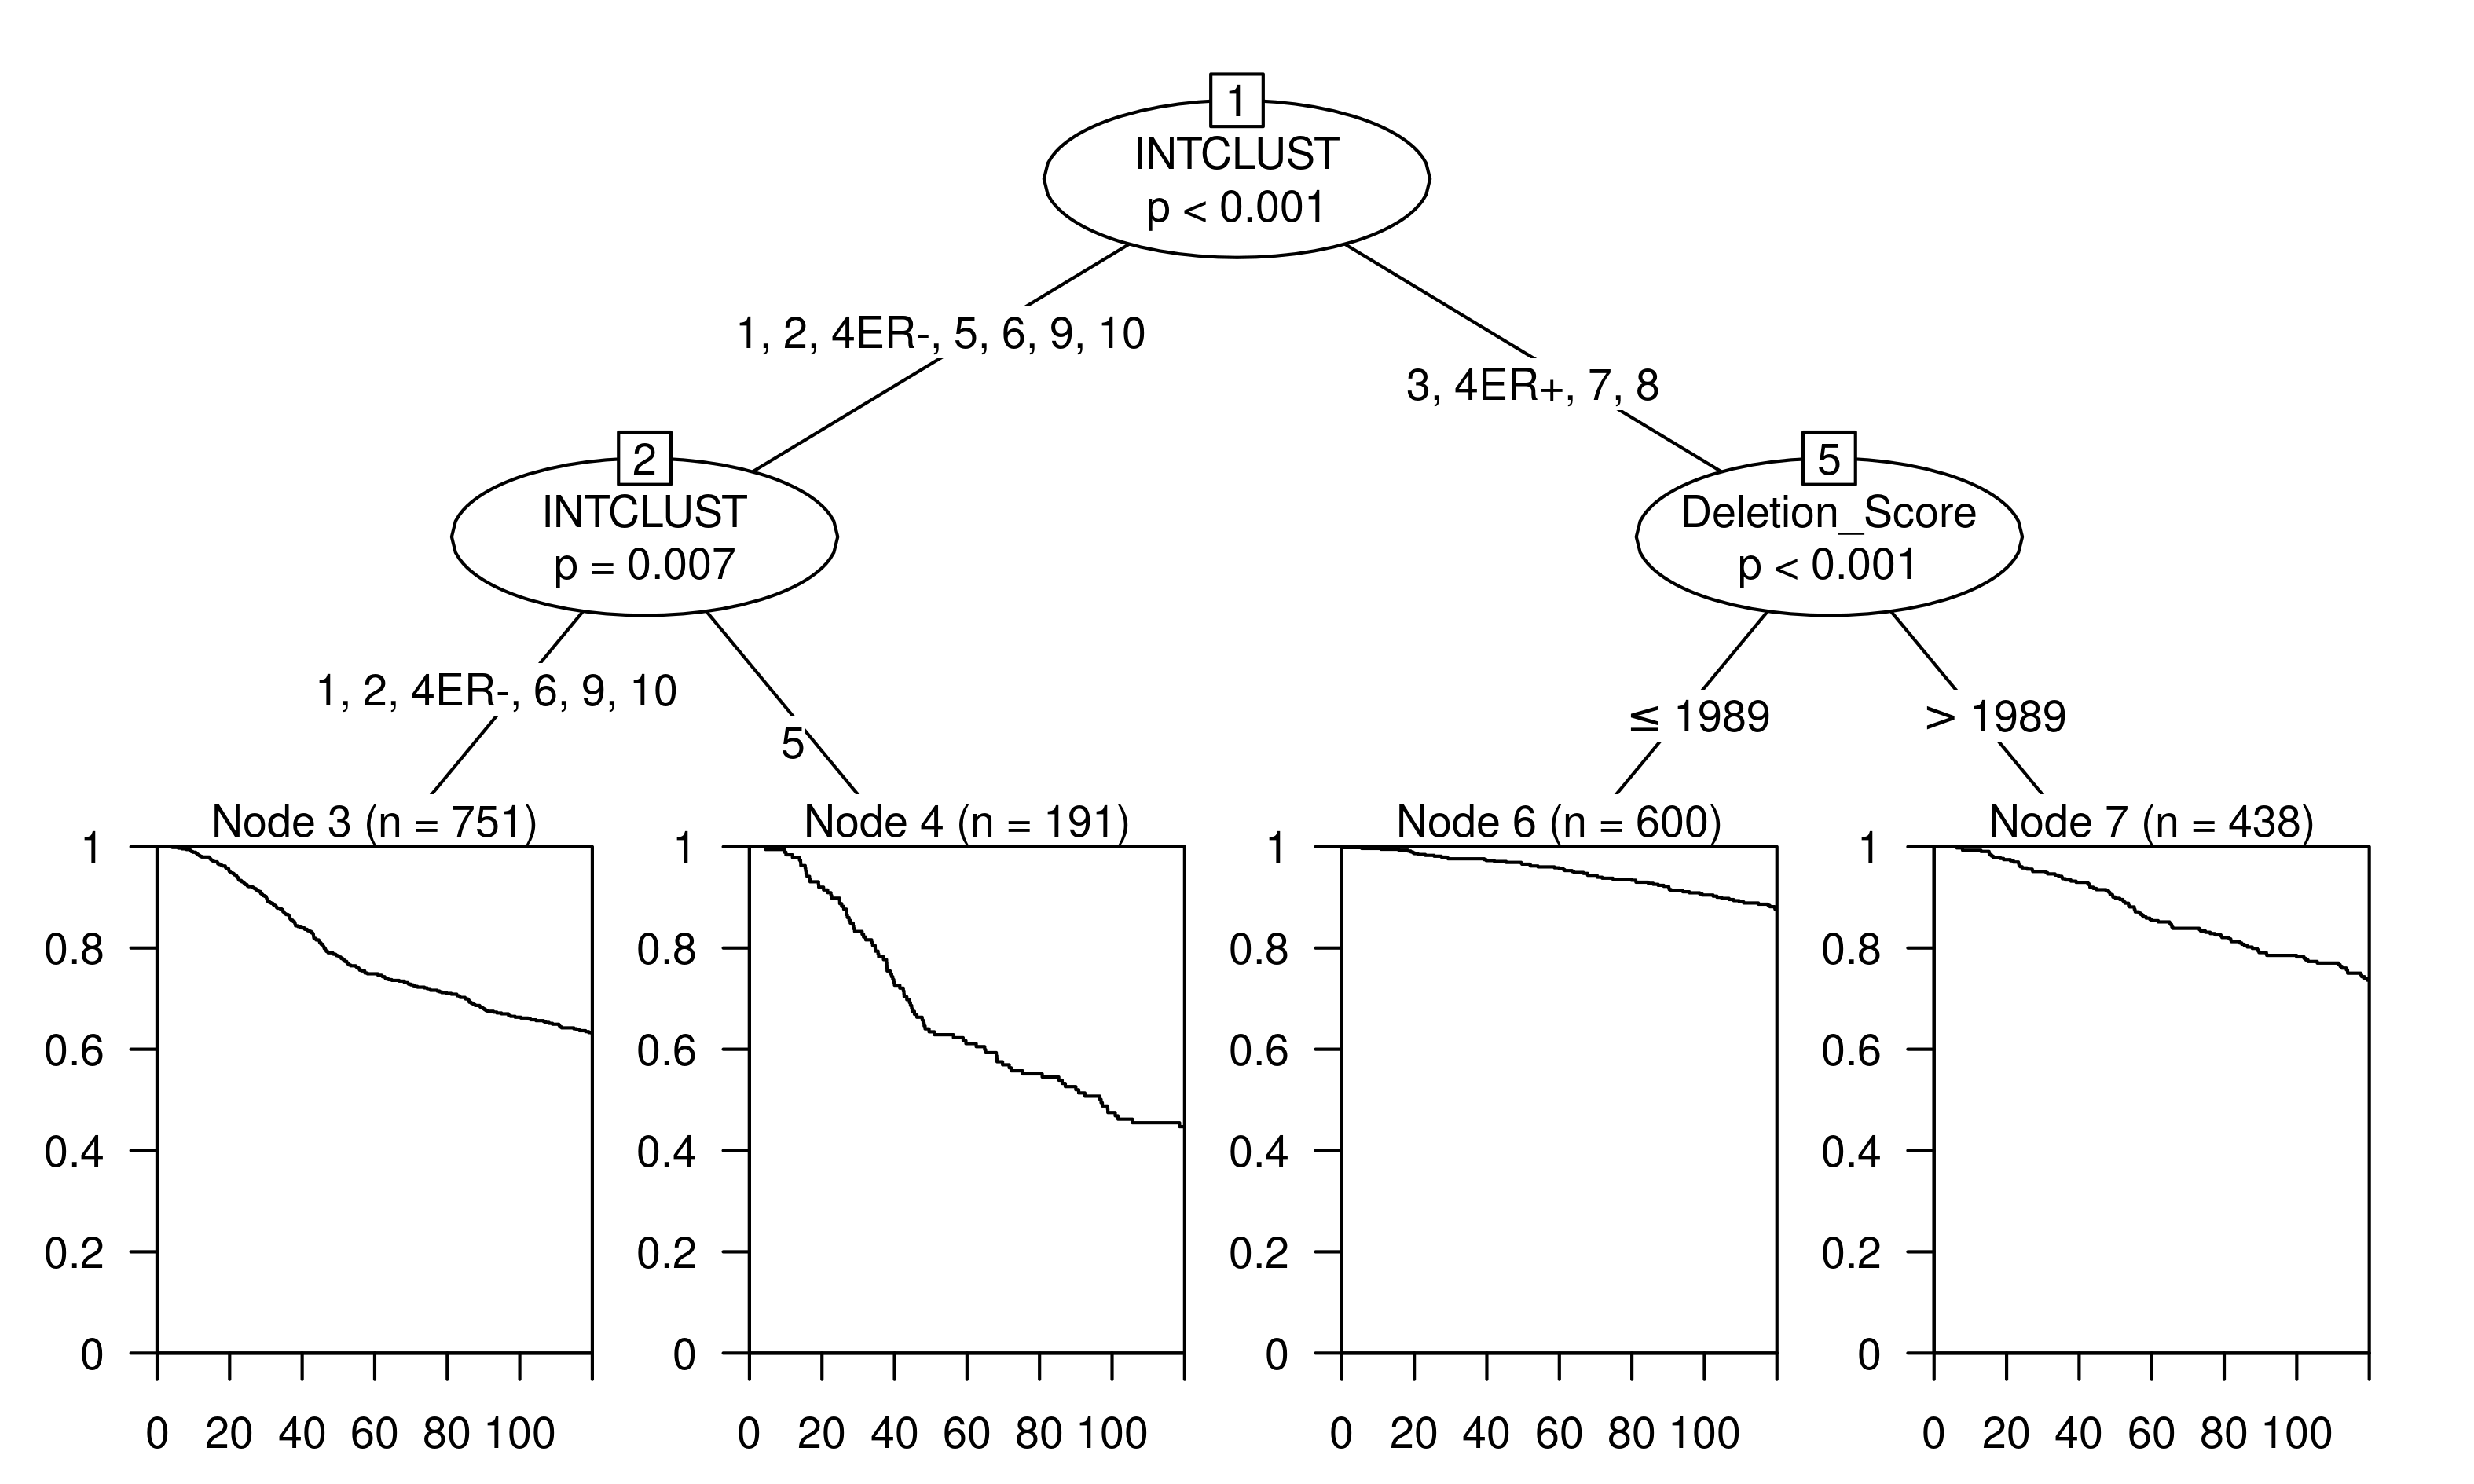
\includegraphics[width=1\textwidth]{../figures/Chapter_3/Ctree_Survival_Score_TenYearDSS_INTCLUST.png}
\end{subfigure}

\vspace{0.5cm}

\caption[Recursive partitioning survival trees for ten-year disease-specific survival using Integrative Cluster and the six CNA Score metrics as candidate predictors.]{Recursive partitioning survival trees for ten-year disease-specific survival using Integrative Cluster and the six CNA Score metrics as candidate predictors. (A) Trees fitted using the rpart algorithm and (B) trees fitted using the ctree algorithm.}
\label{fig:INTCLUST_CNA_Score_TenYearDSS}
\end{figure}

\begin{figure}[!h]
\centering

\vspace{0.5cm}

\begin{subfigure}{\textwidth}
\subcaption{}
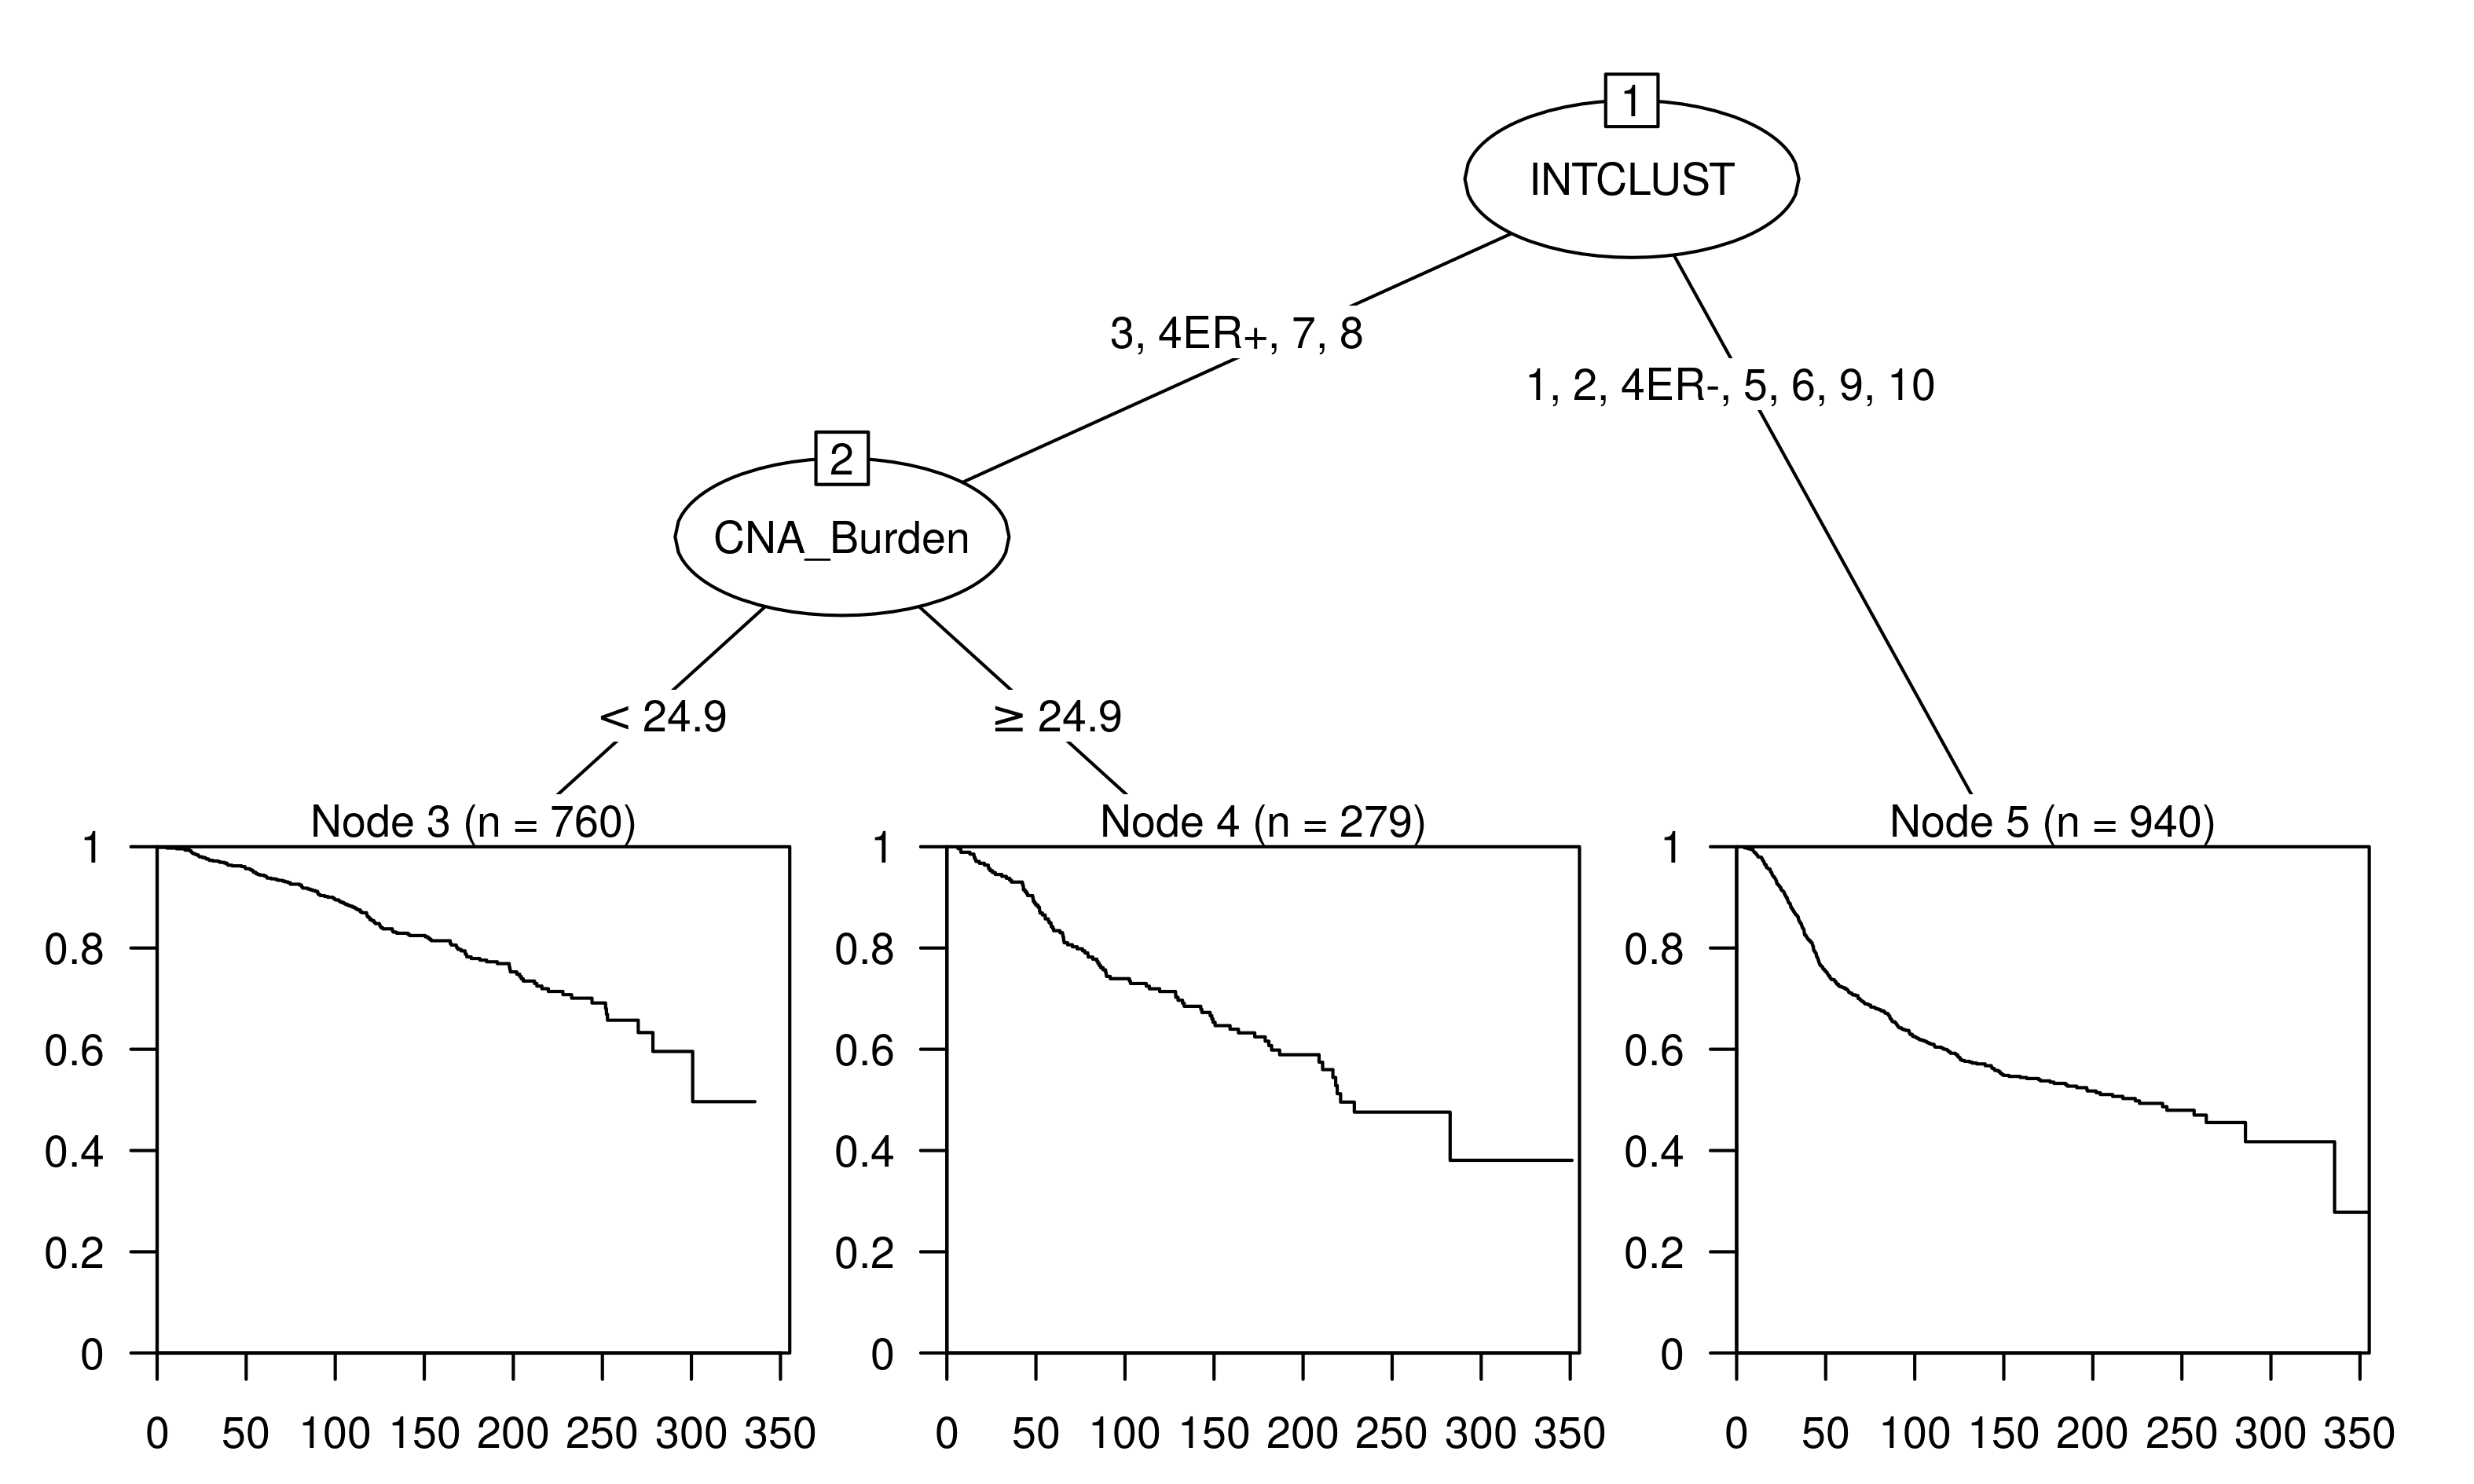
\includegraphics[width=1\textwidth]{../figures/Chapter_3/PartyKit_Survival_Burden_DSS_INTCLUST.png}
\end{subfigure}

\vspace{2cm}

\begin{subfigure}{\textwidth}
\subcaption{}
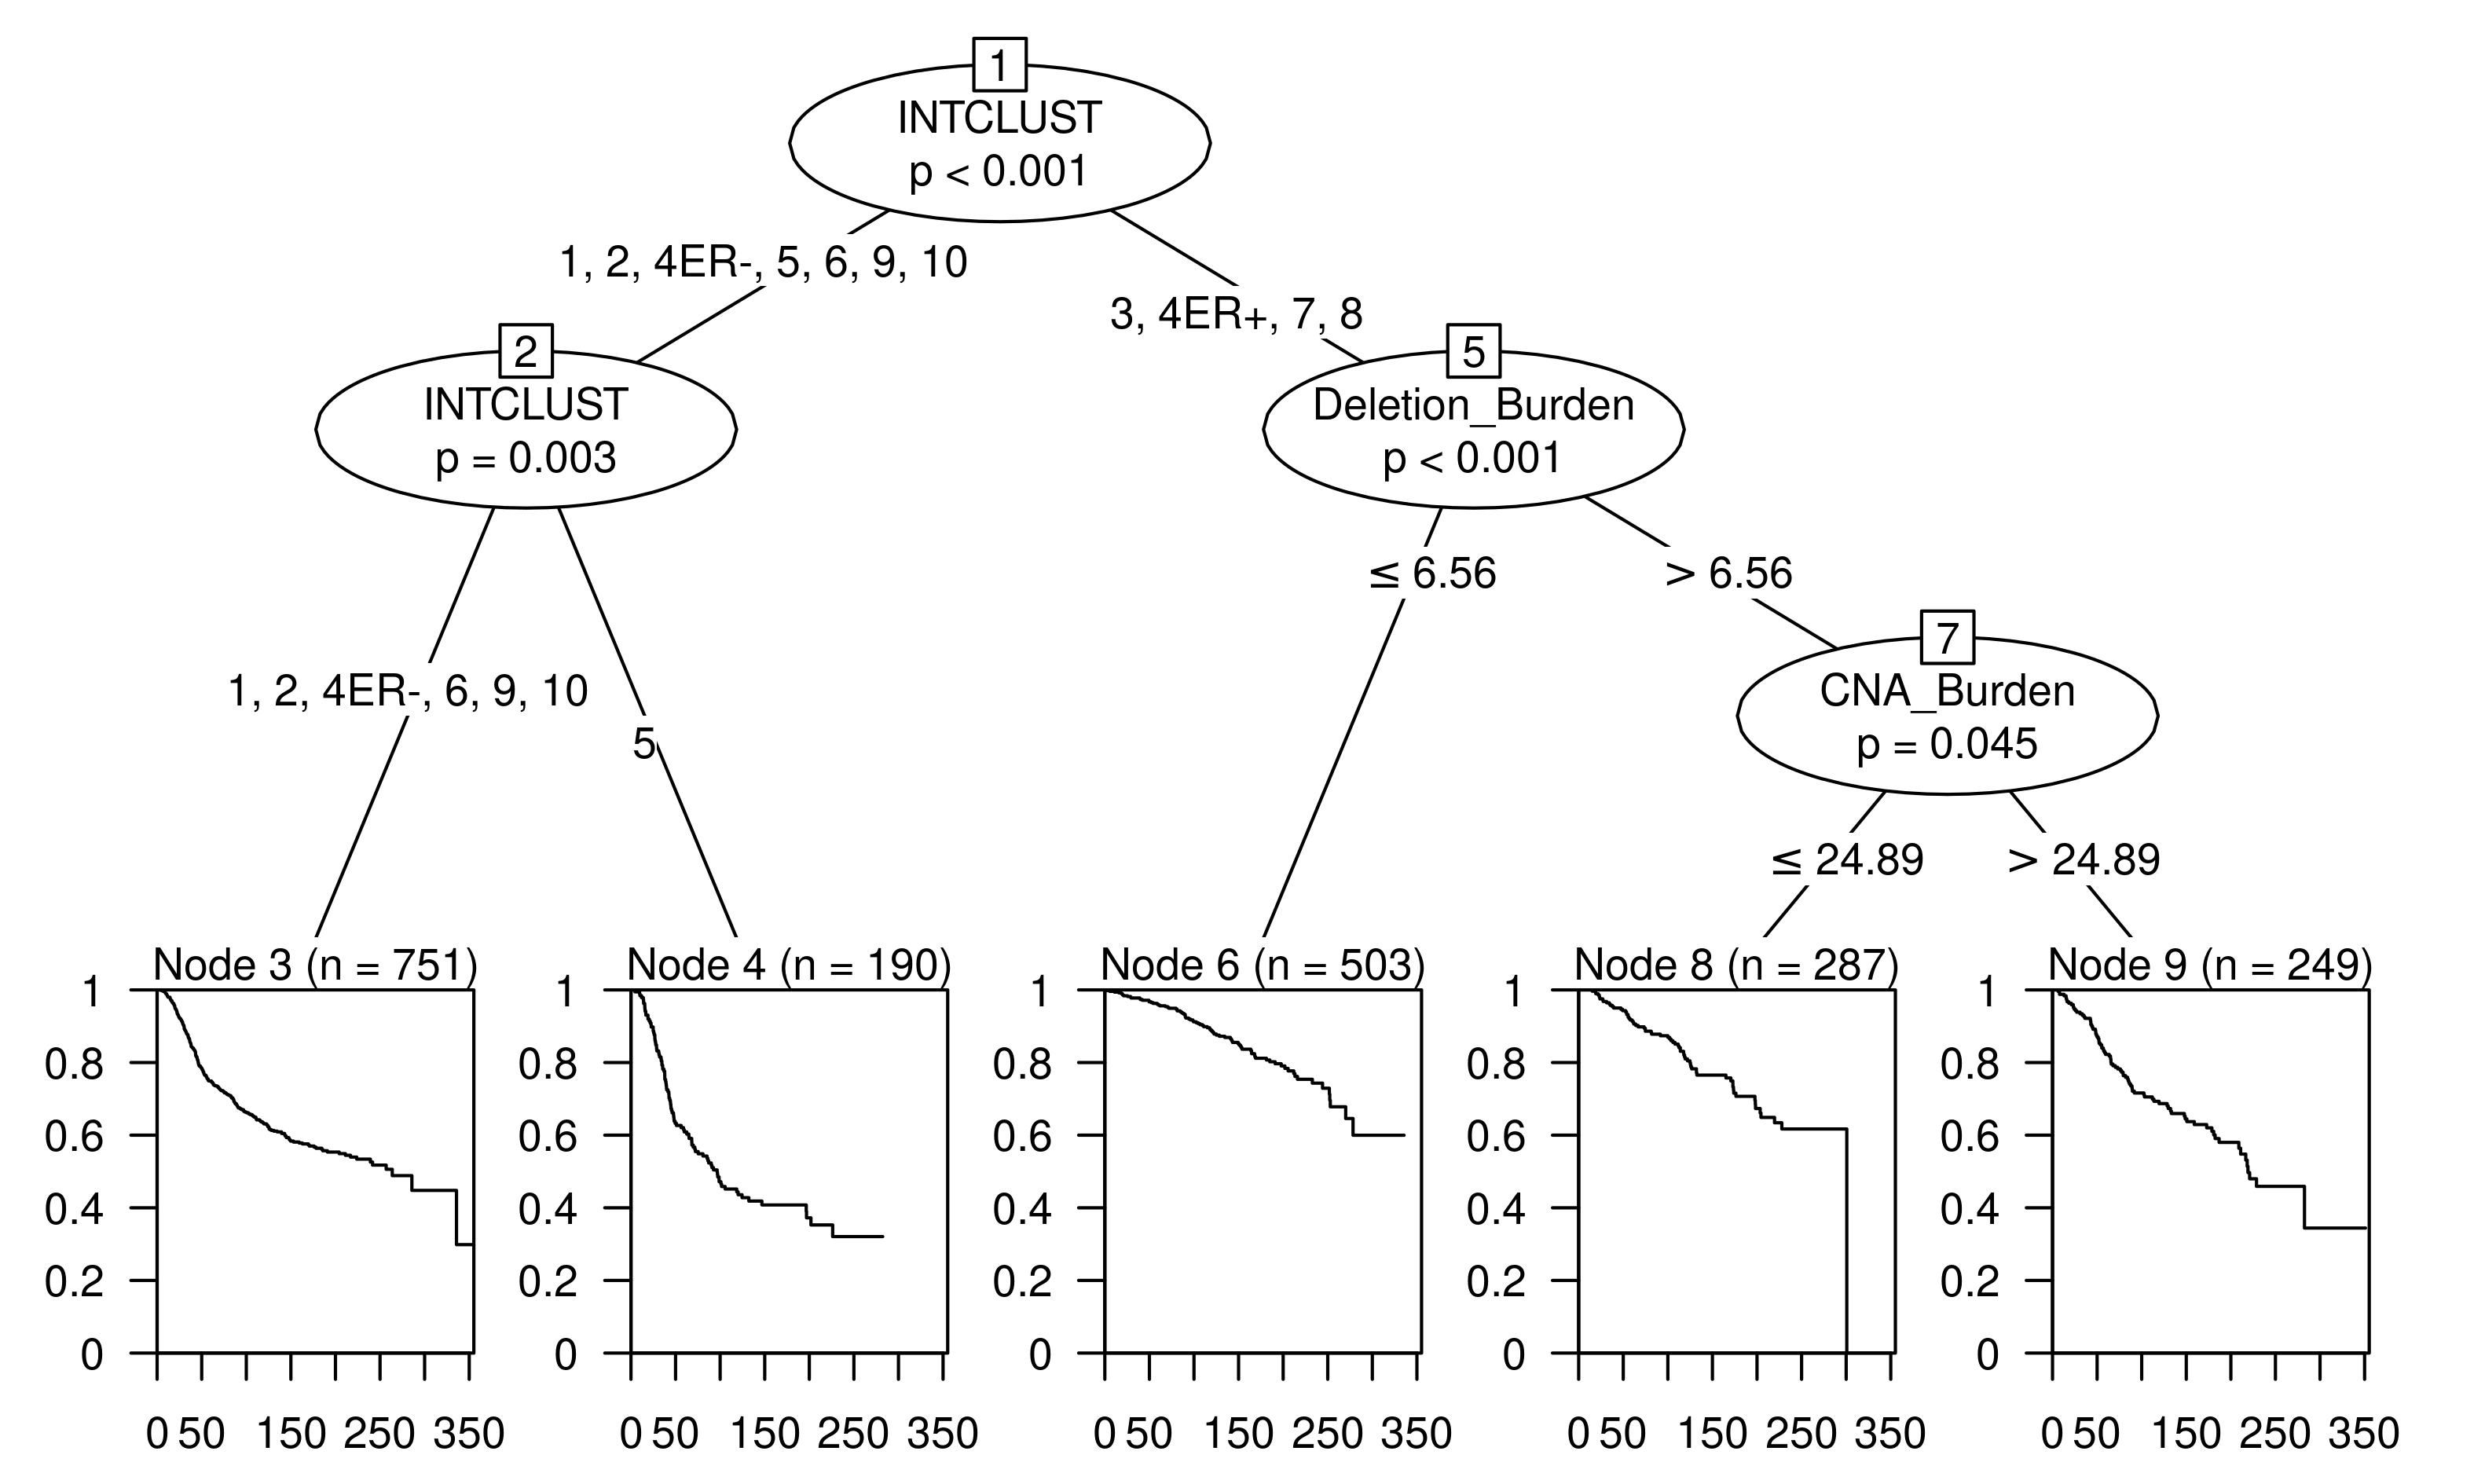
\includegraphics[width=1\textwidth]{../figures/Chapter_3/Ctree_Survival_Burden_DSS_INTCLUST.png}
\end{subfigure}

\vspace{0.5cm}

\caption[Recursive partitioning survival trees for disease-specific survival using Integrative Cluster and the six CNA Burden metrics as candidate predictors.]{Recursive partitioning survival trees for disease-specific survival using Integrative Cluster and the six CNA Burden metrics as candidate predictors. (A) Trees fitted using the rpart algorithm and (B) trees fitted using the ctree algorithm.}
\label{fig:INTCLUST_CNA_Burden_DSS}
\end{figure}

\begin{figure}[!h]
\centering

\vspace{0.5cm}

\begin{subfigure}{\textwidth}
\subcaption{}
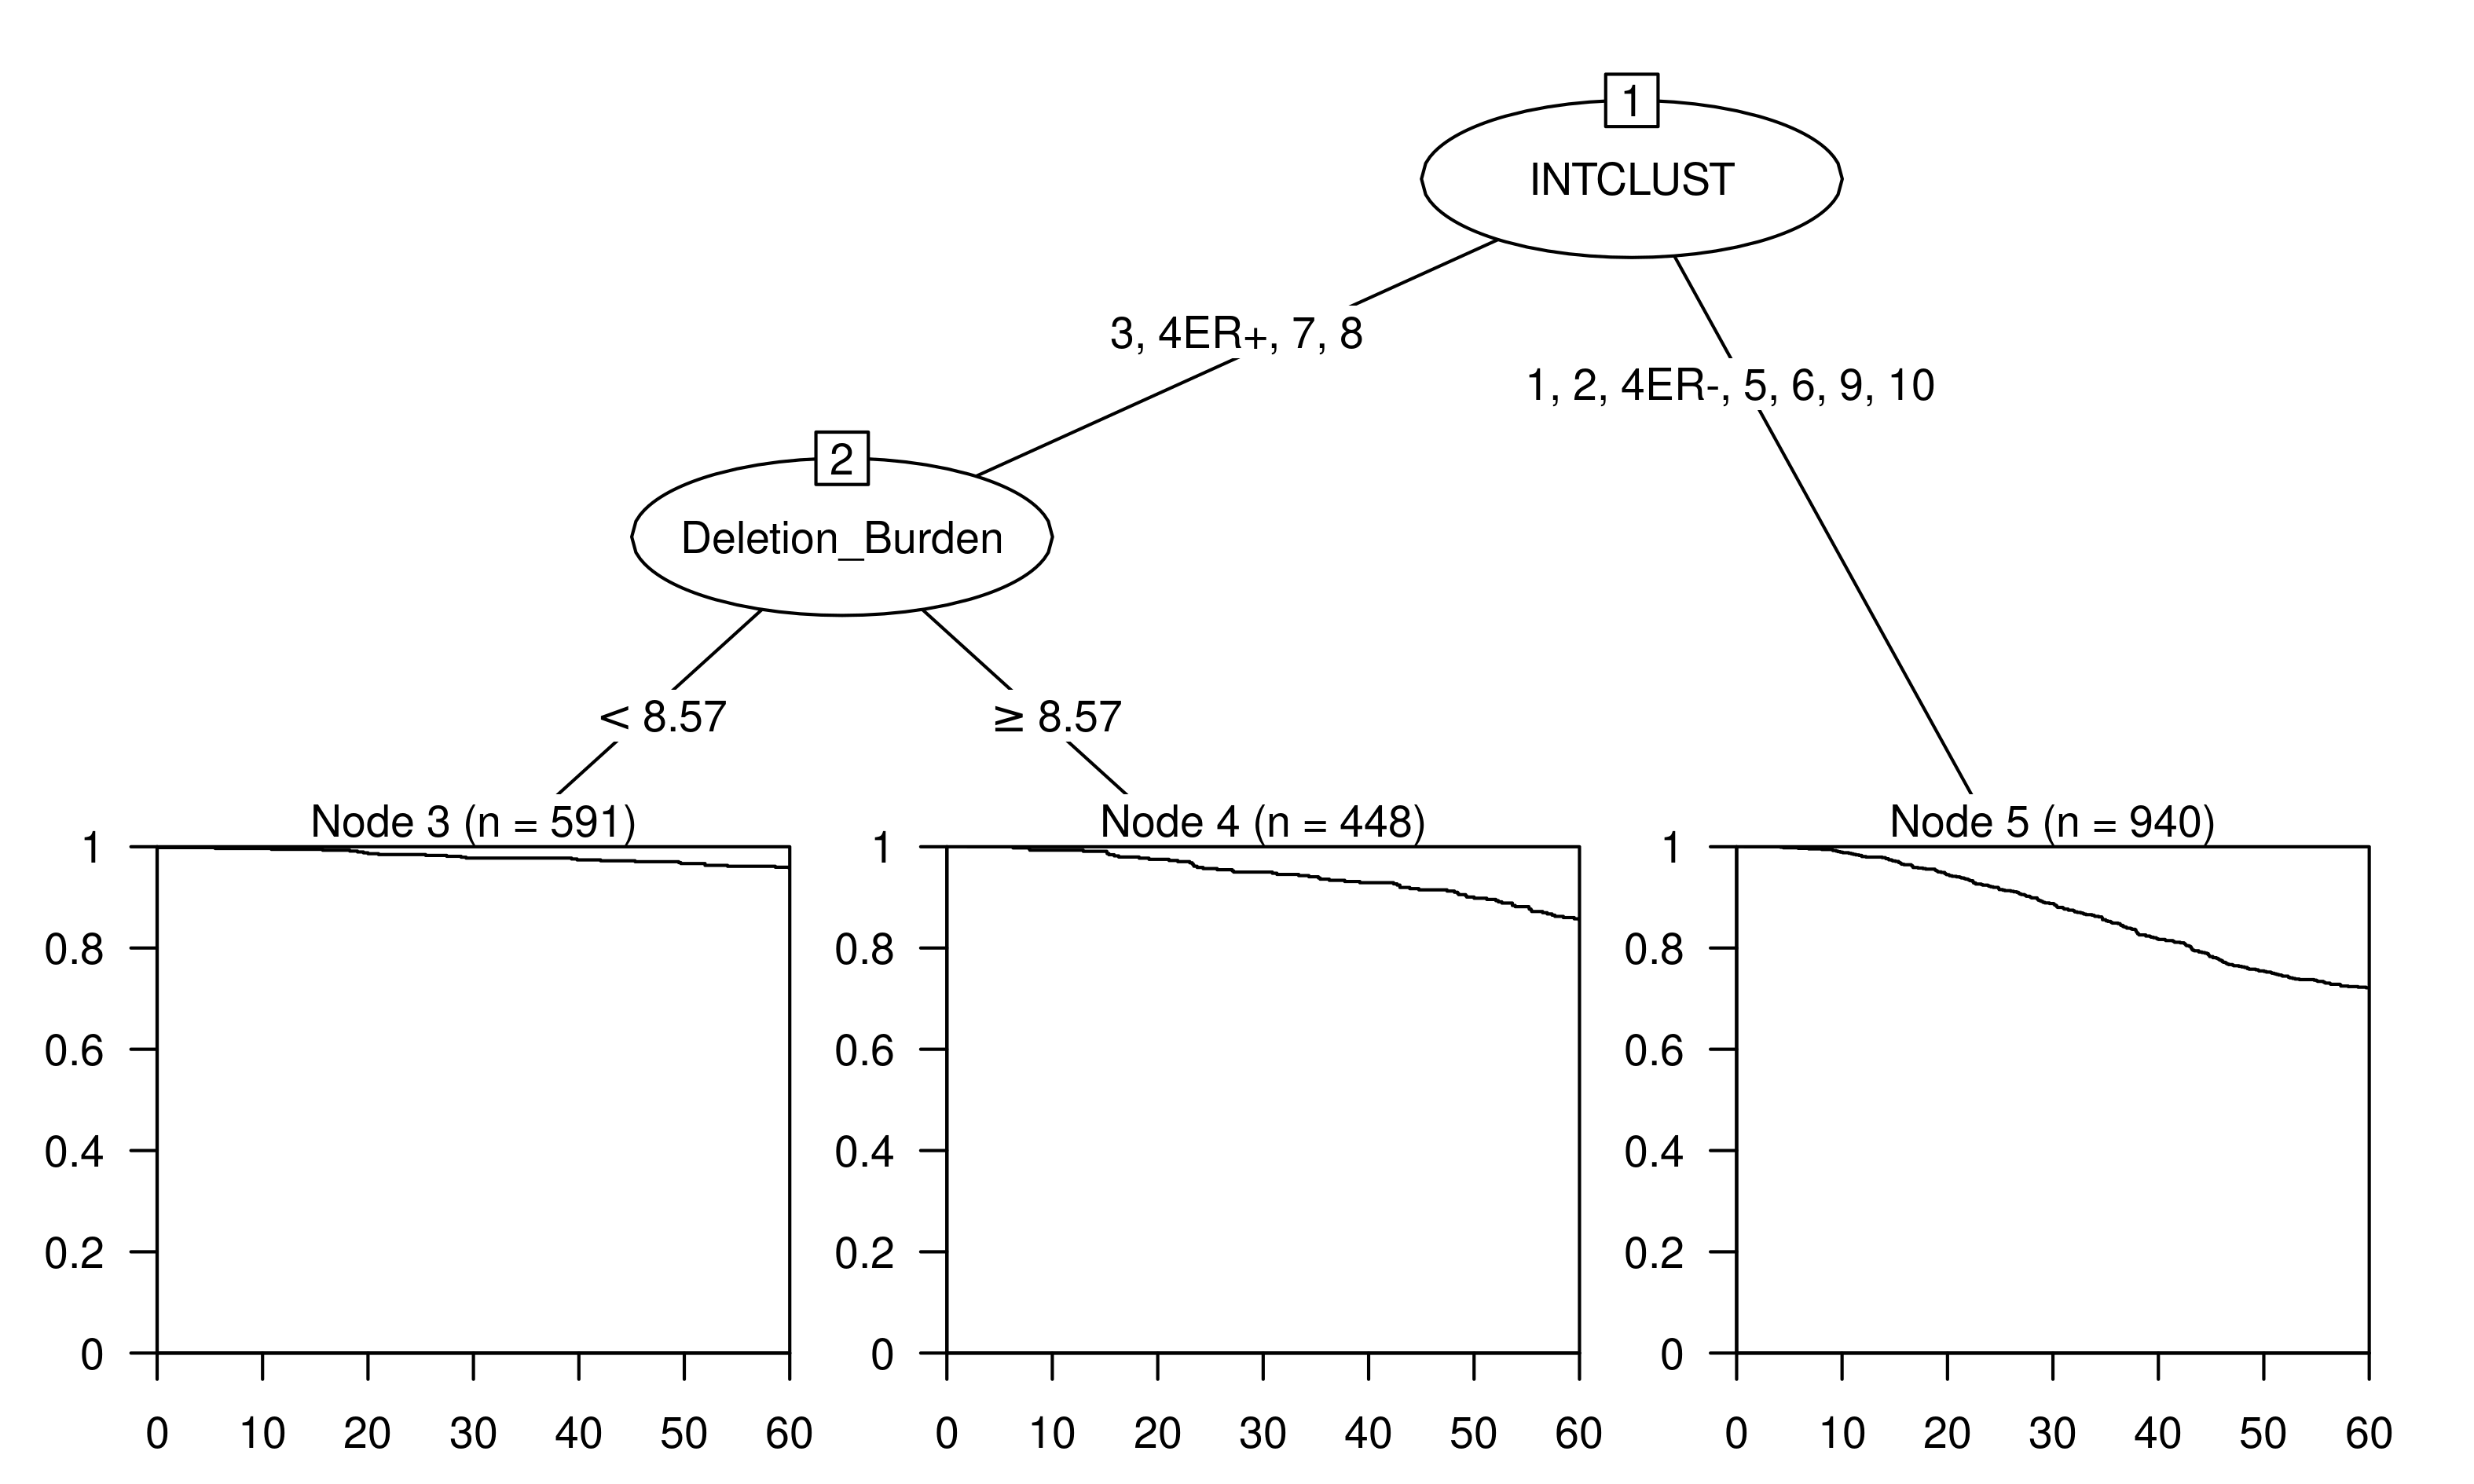
\includegraphics[width=1\textwidth]{../figures/Chapter_3/PartyKit_Survival_Burden_FiveYearDSS_INTCLUST.png}
\end{subfigure}

\vspace{2cm}

\begin{subfigure}{\textwidth}
\subcaption{}
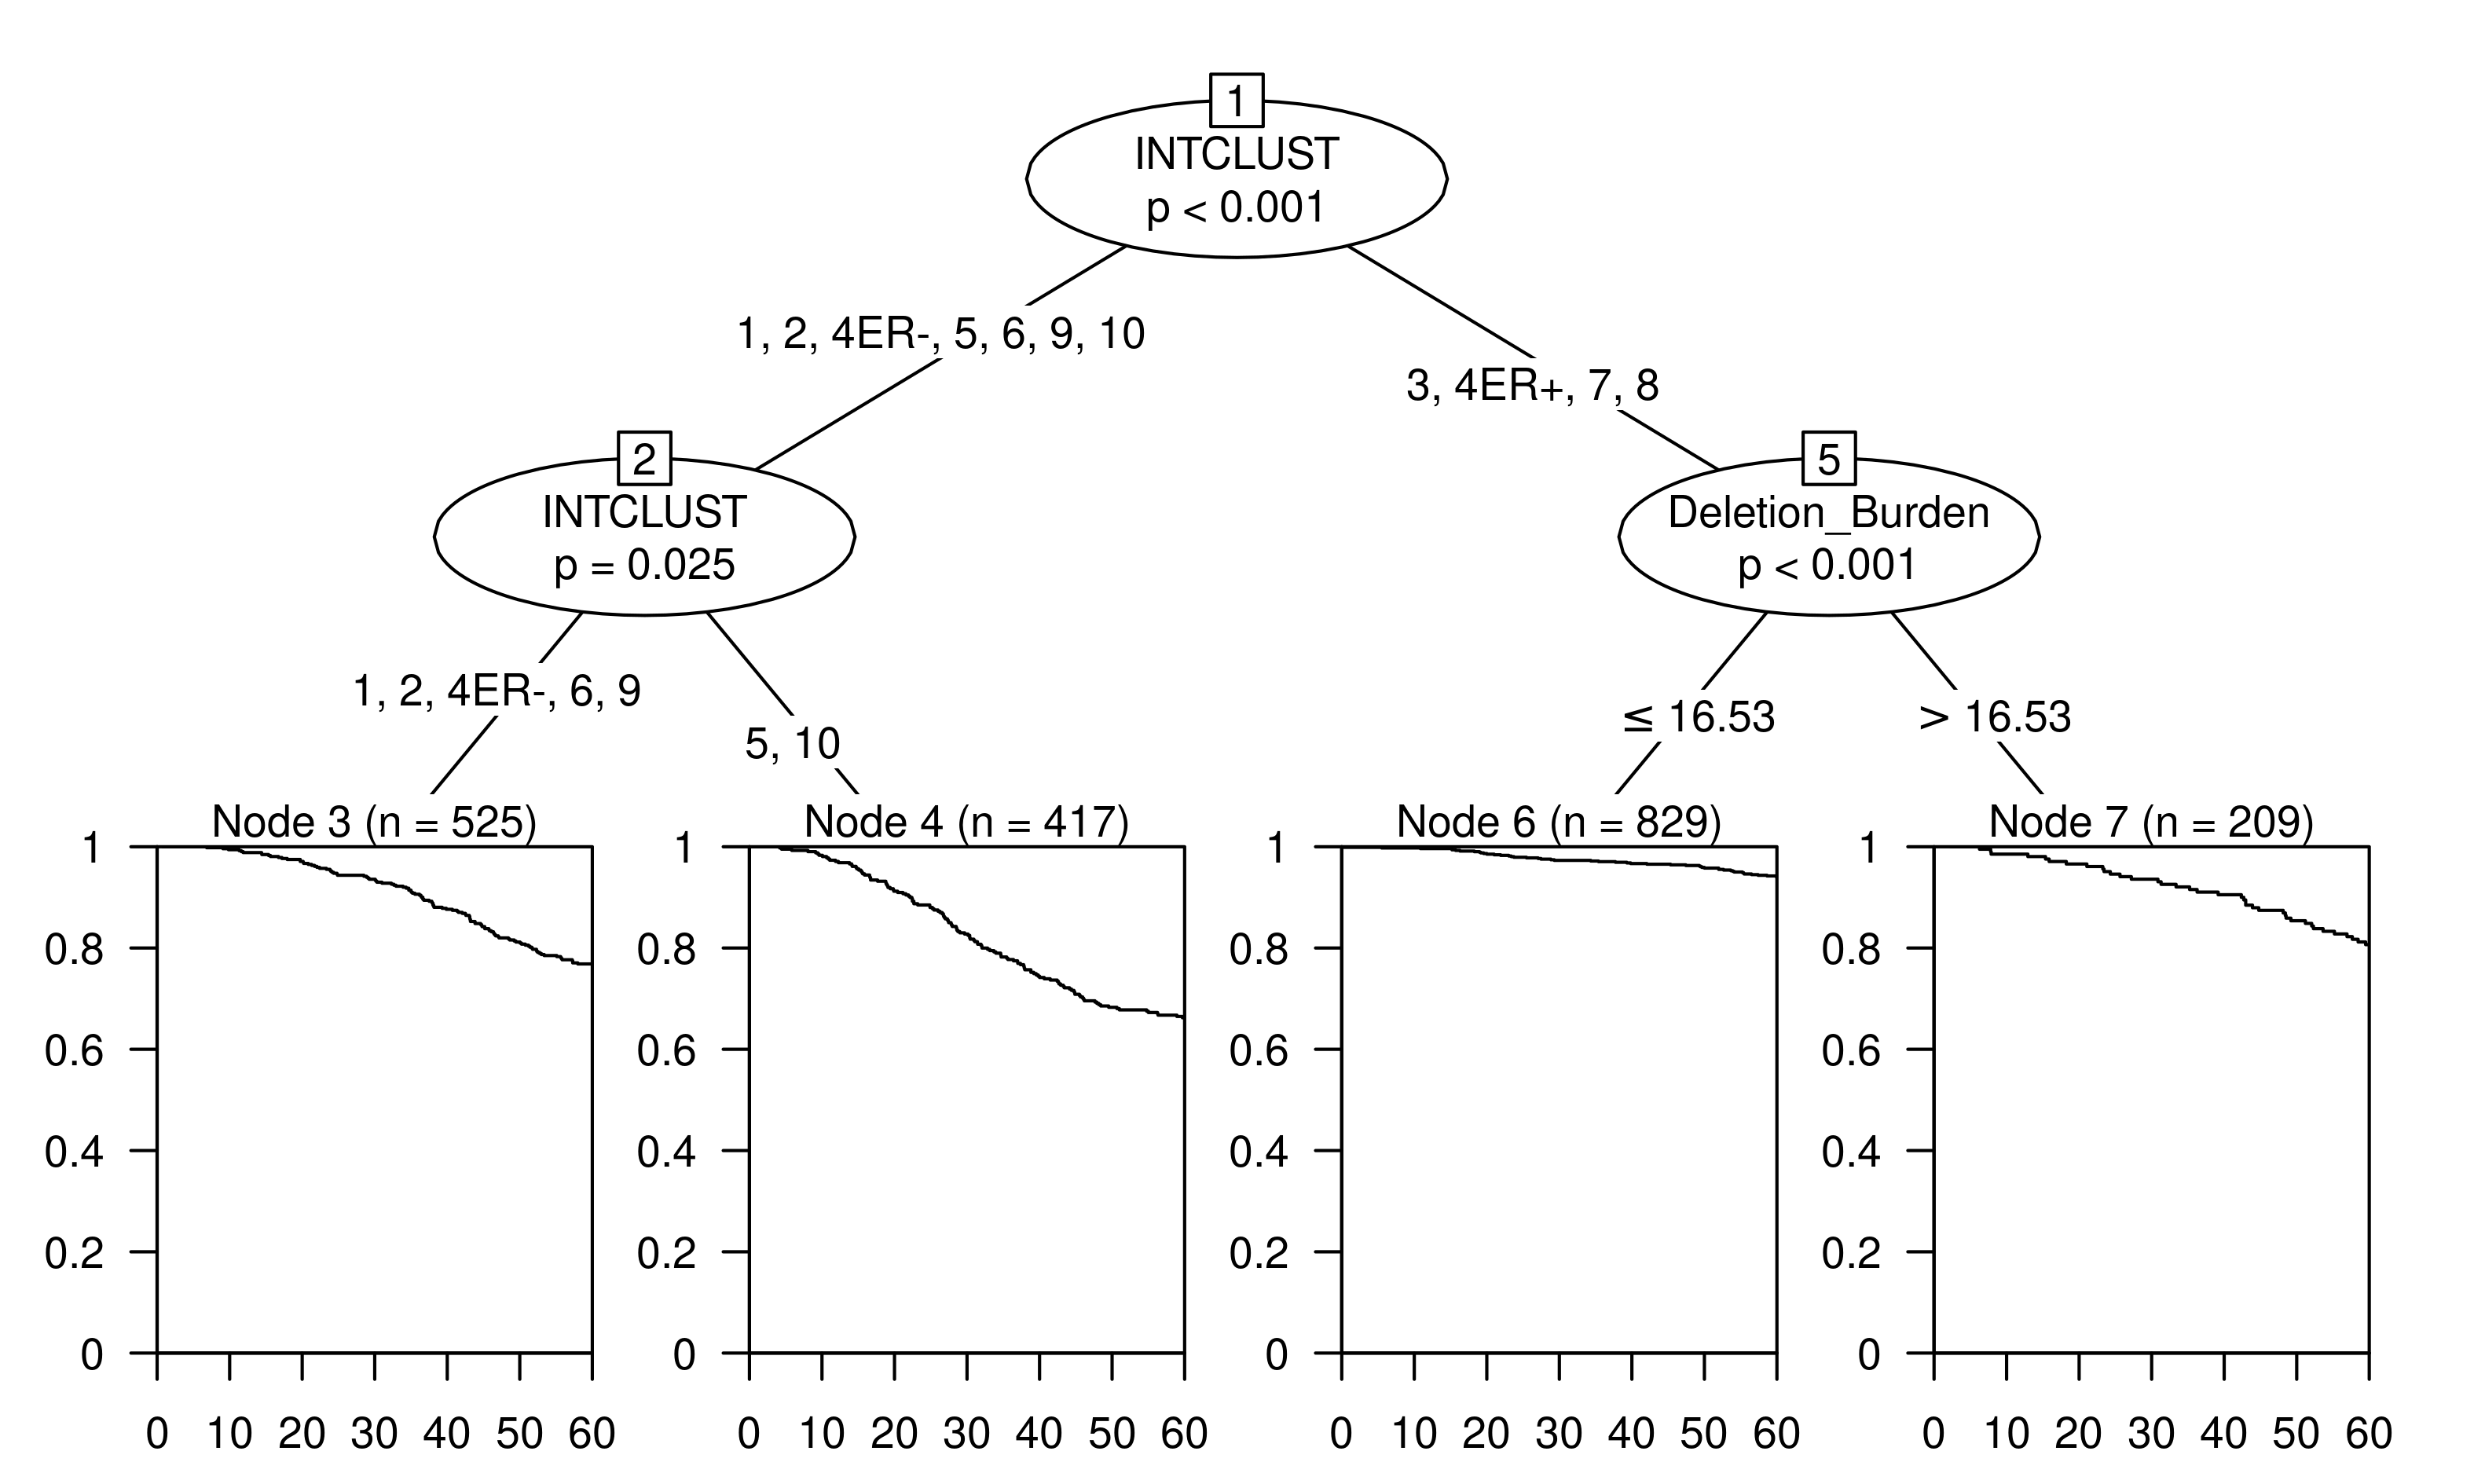
\includegraphics[width=1\textwidth]{../figures/Chapter_3/Ctree_Survival_Burden_FiveYearDSS_INTCLUST.png}
\end{subfigure}

\vspace{0.5cm}

\caption[Recursive partitioning survival trees for five-year disease-specific survival using Integrative Cluster and the six CNA Burden metrics as candidate predictors.]{Recursive partitioning survival trees for five-year disease-specific survival using Integrative Cluster and the six CNA Burden metrics as candidate predictors. (A) Trees fitted using the rpart algorithm and (B) trees fitted using the ctree algorithm.}
\label{fig:INTCLUST_CNA_Burden_FiveYearDSS}
\end{figure}

\begin{figure}[!h]
\centering

\vspace{0.5cm}

\begin{subfigure}{\textwidth}
\subcaption{}
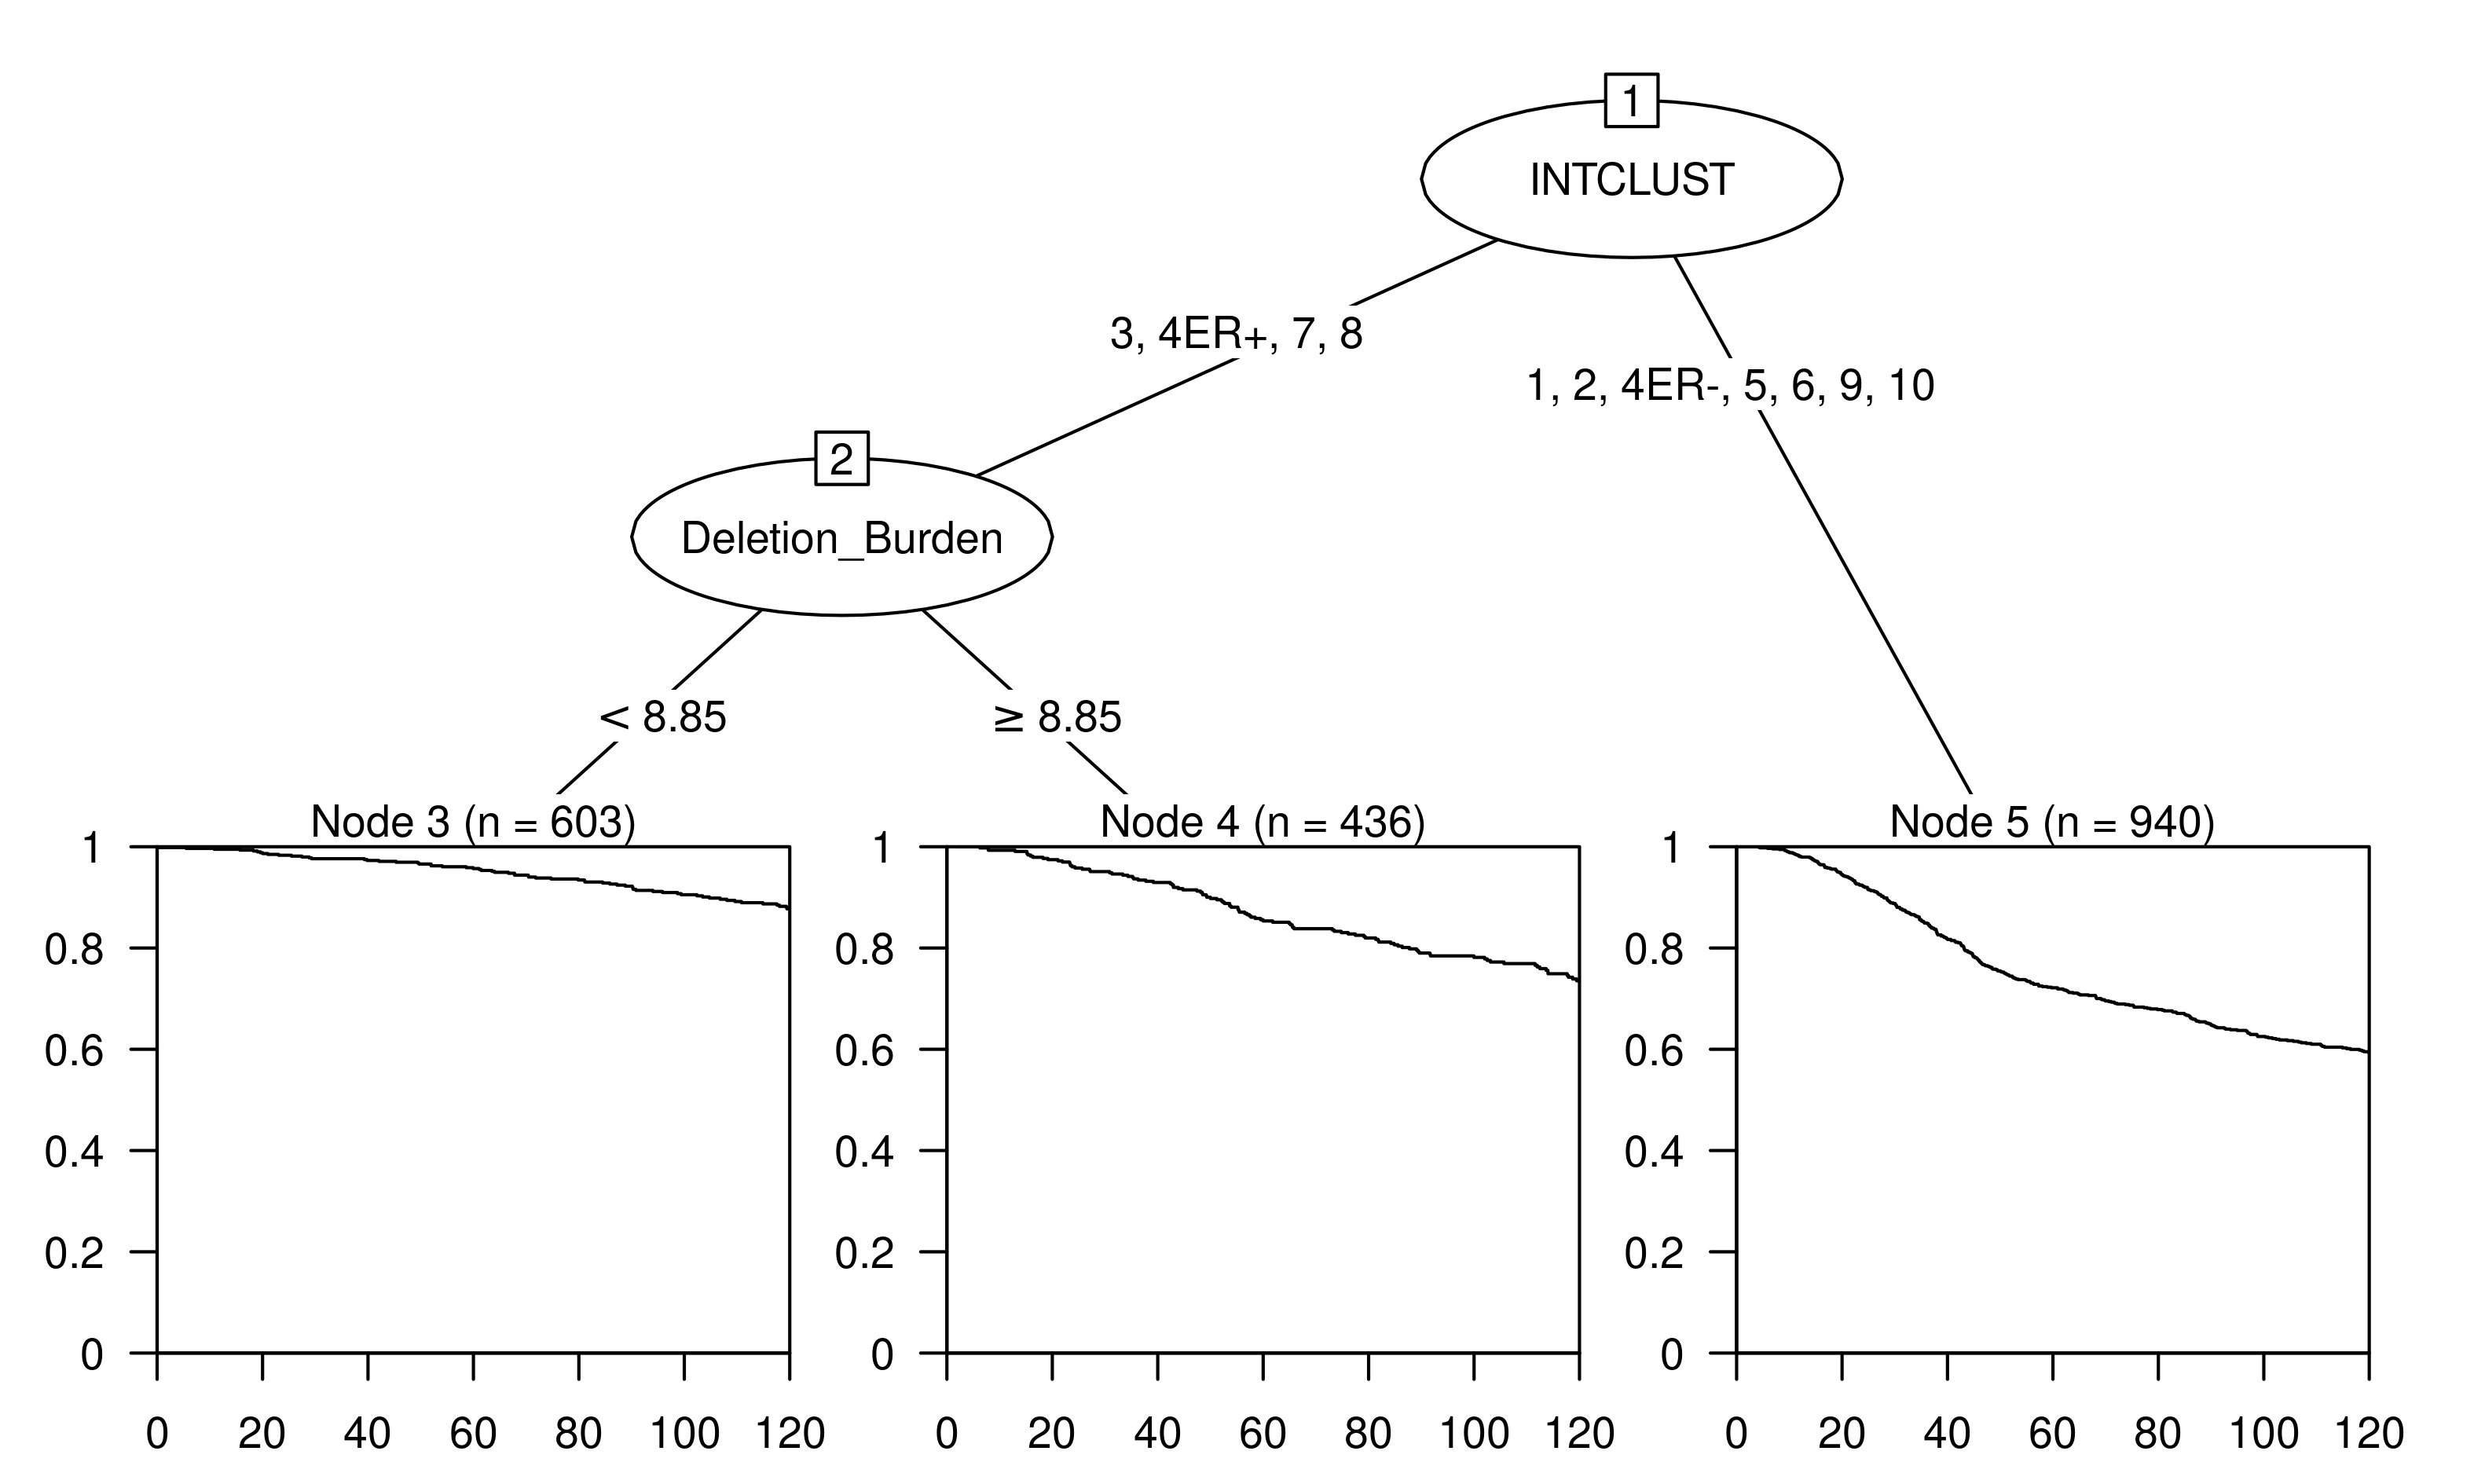
\includegraphics[width=1\textwidth]{../figures/Chapter_3/PartyKit_Survival_Burden_TenYearDSS_INTCLUST.png}
\end{subfigure}

\vspace{2cm}

\begin{subfigure}{\textwidth}
\subcaption{}
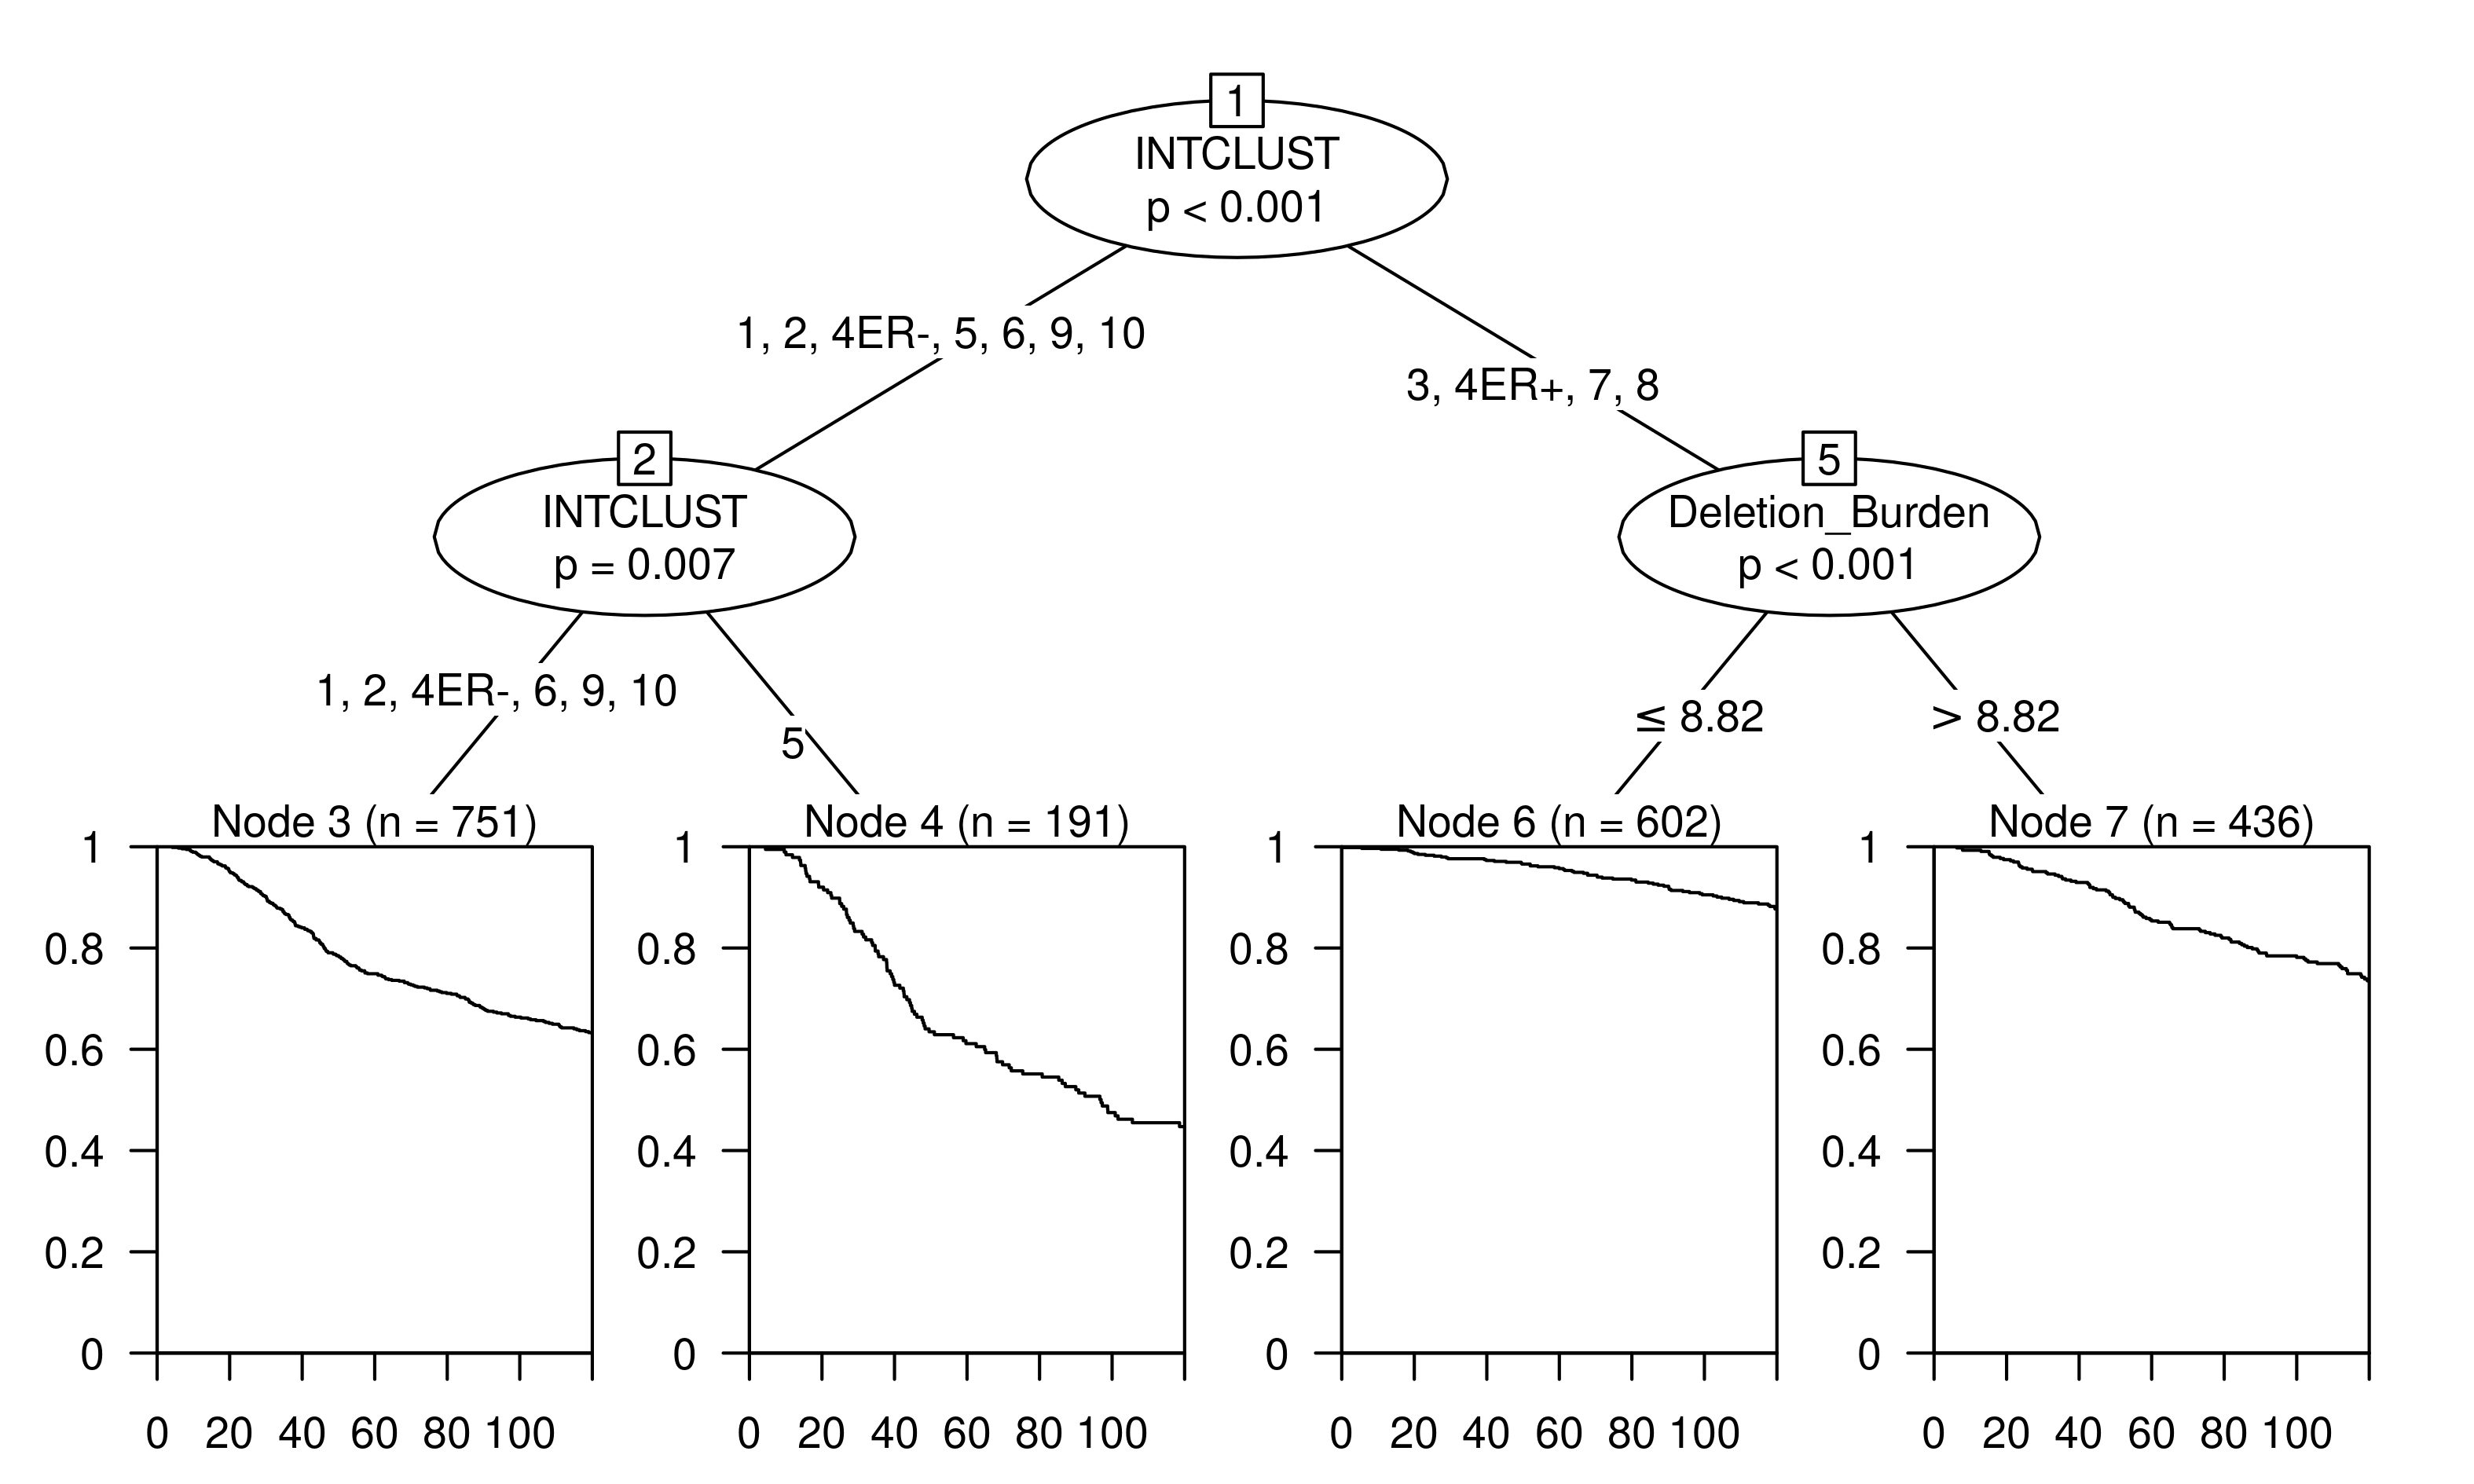
\includegraphics[width=1\textwidth]{../figures/Chapter_3/Ctree_Survival_Burden_TenYearDSS_INTCLUST.png}
\end{subfigure}

\vspace{0.5cm}

\caption[Recursive partitioning survival trees for ten-year disease-specific survival using Integrative Cluster and the six CNA Burden metrics as candidate predictors.]{Recursive partitioning survival trees for ten-year disease-specific survival using Integrative Cluster and the six CNA Burden metrics as candidate predictors. (A) Trees fitted using the rpart algorithm and (B) trees fitted using the ctree algorithm.}
\label{fig:INTCLUST_CNA_Burden_TenYearDSS}
\end{figure}


\begin{figure}[!h]
\centering

\vspace{1cm}

\begin{subfigure}{\textwidth}
\subcaption{}
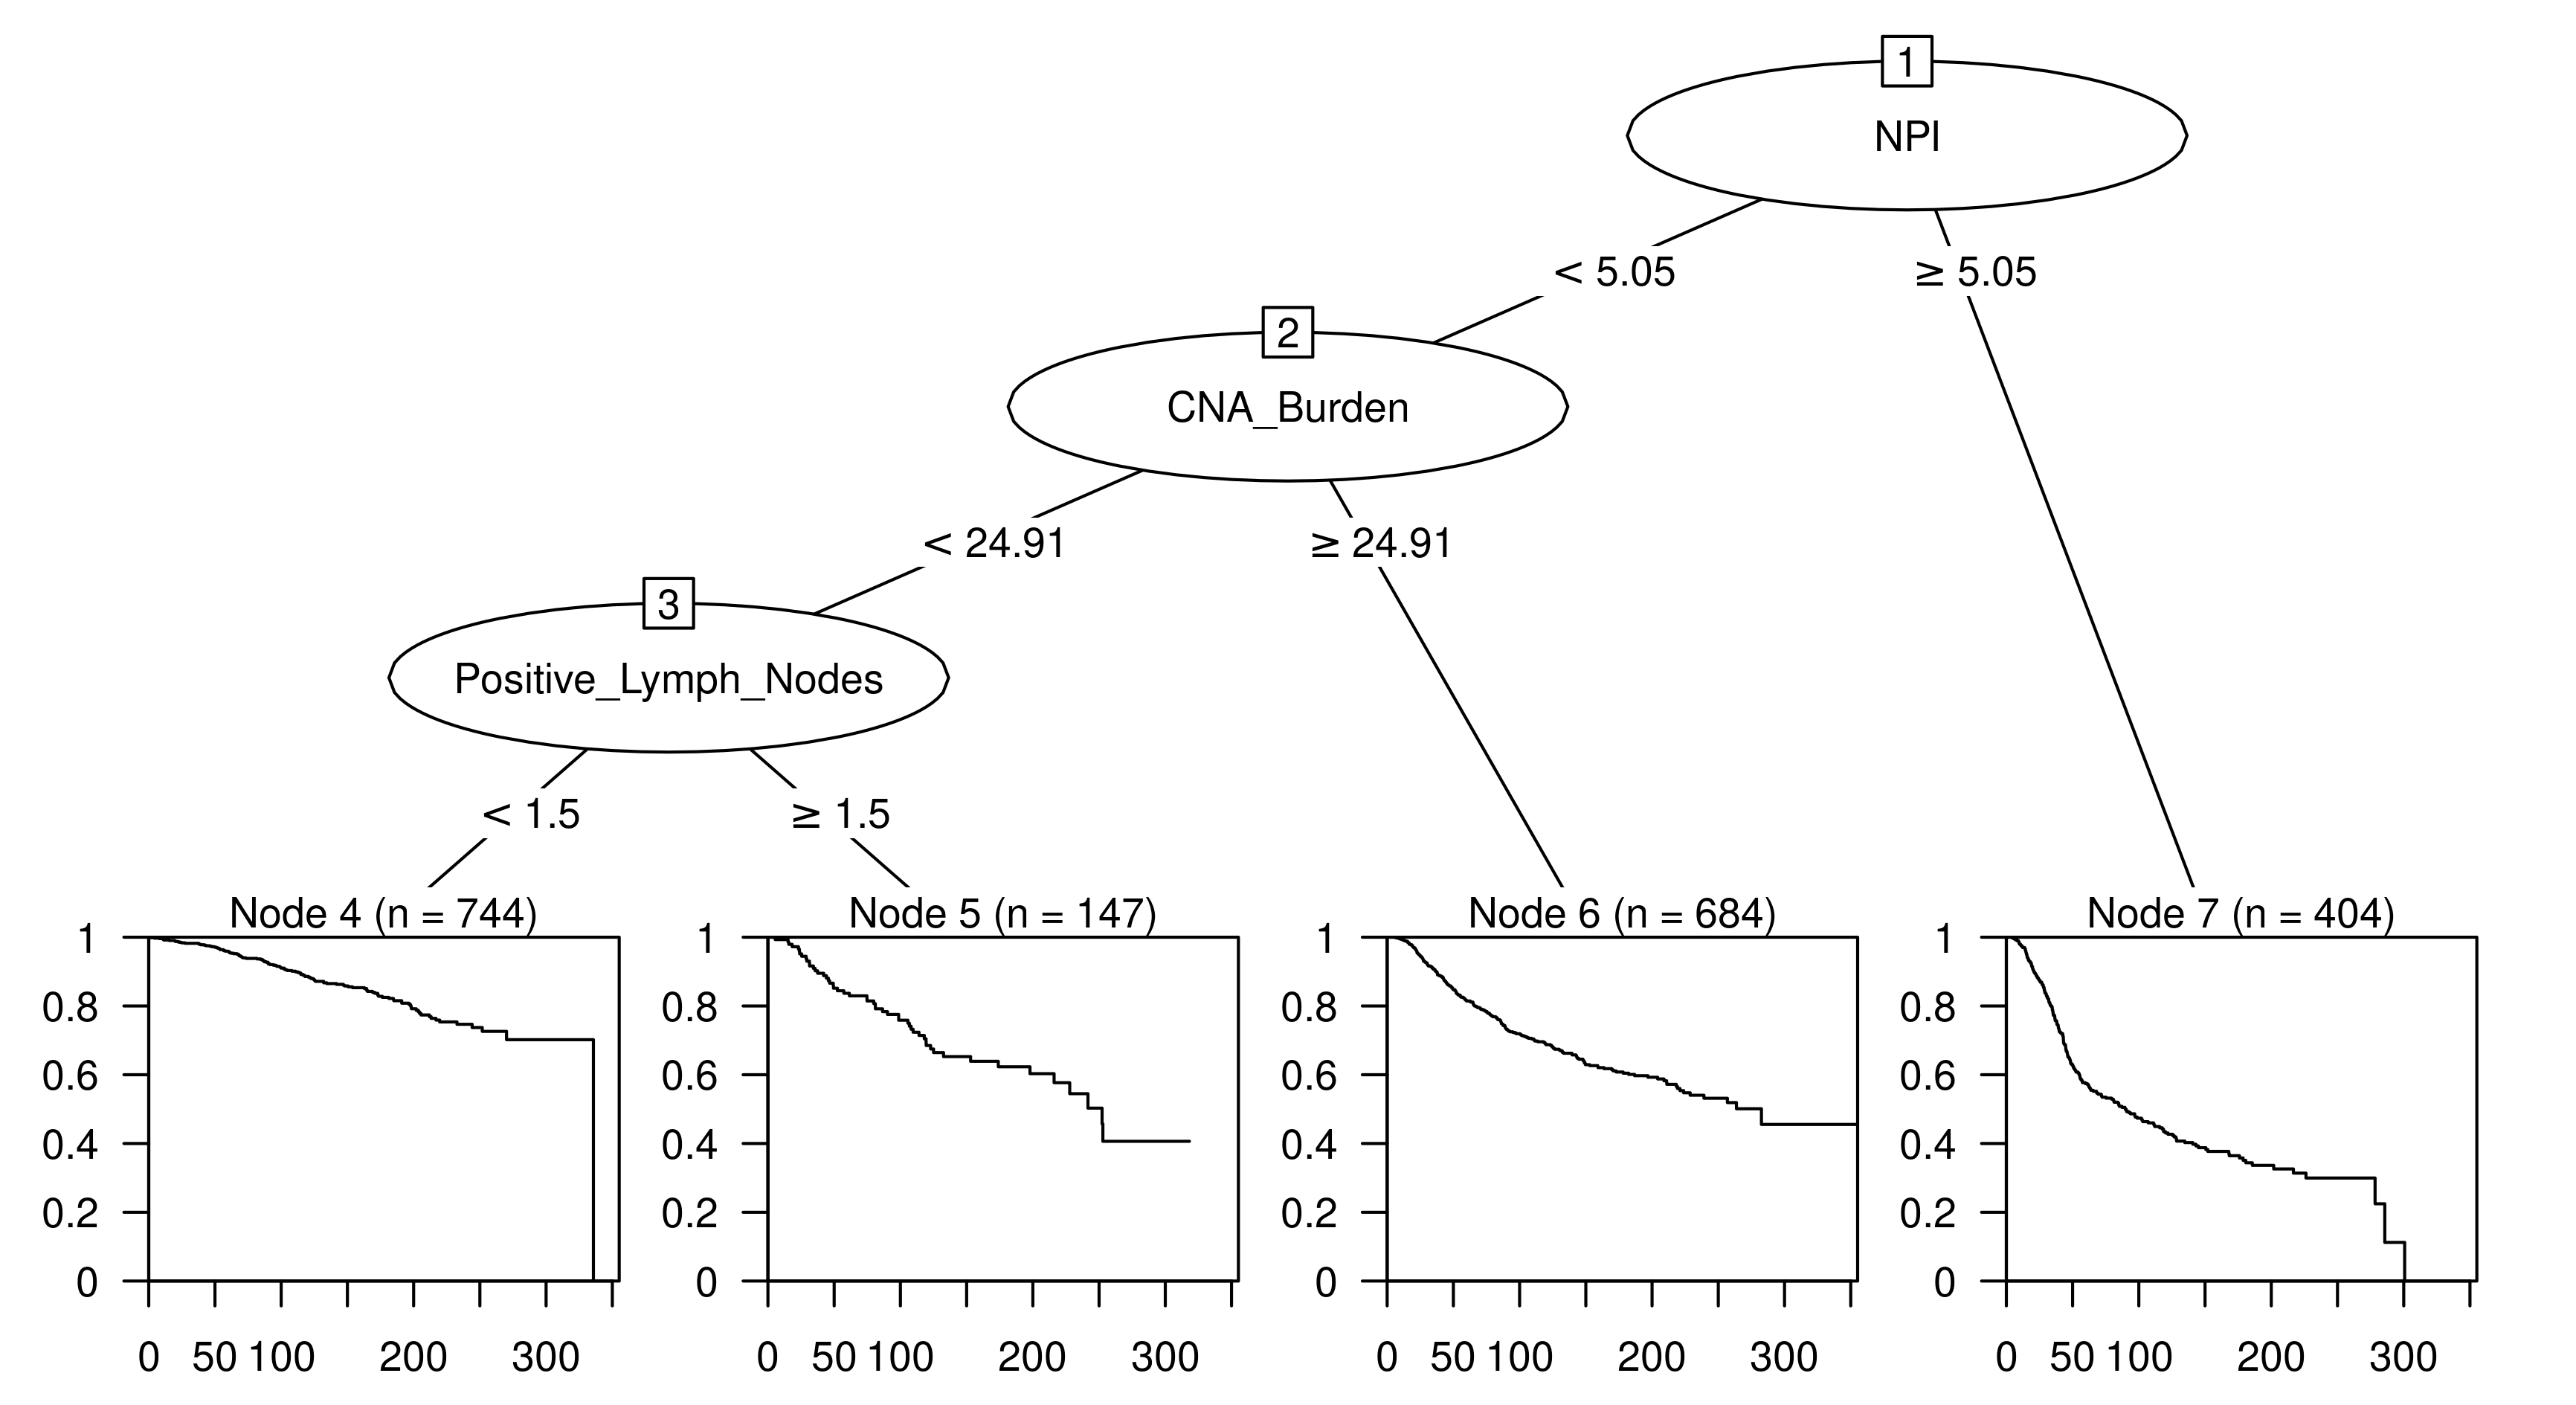
\includegraphics[width=1\textwidth]{../figures/Chapter_3/Clin_PartyKit_Survival_Burden_DSS_PAM50.png}
\end{subfigure}

\vspace{3cm}

\begin{subfigure}{\textwidth}
\subcaption{}
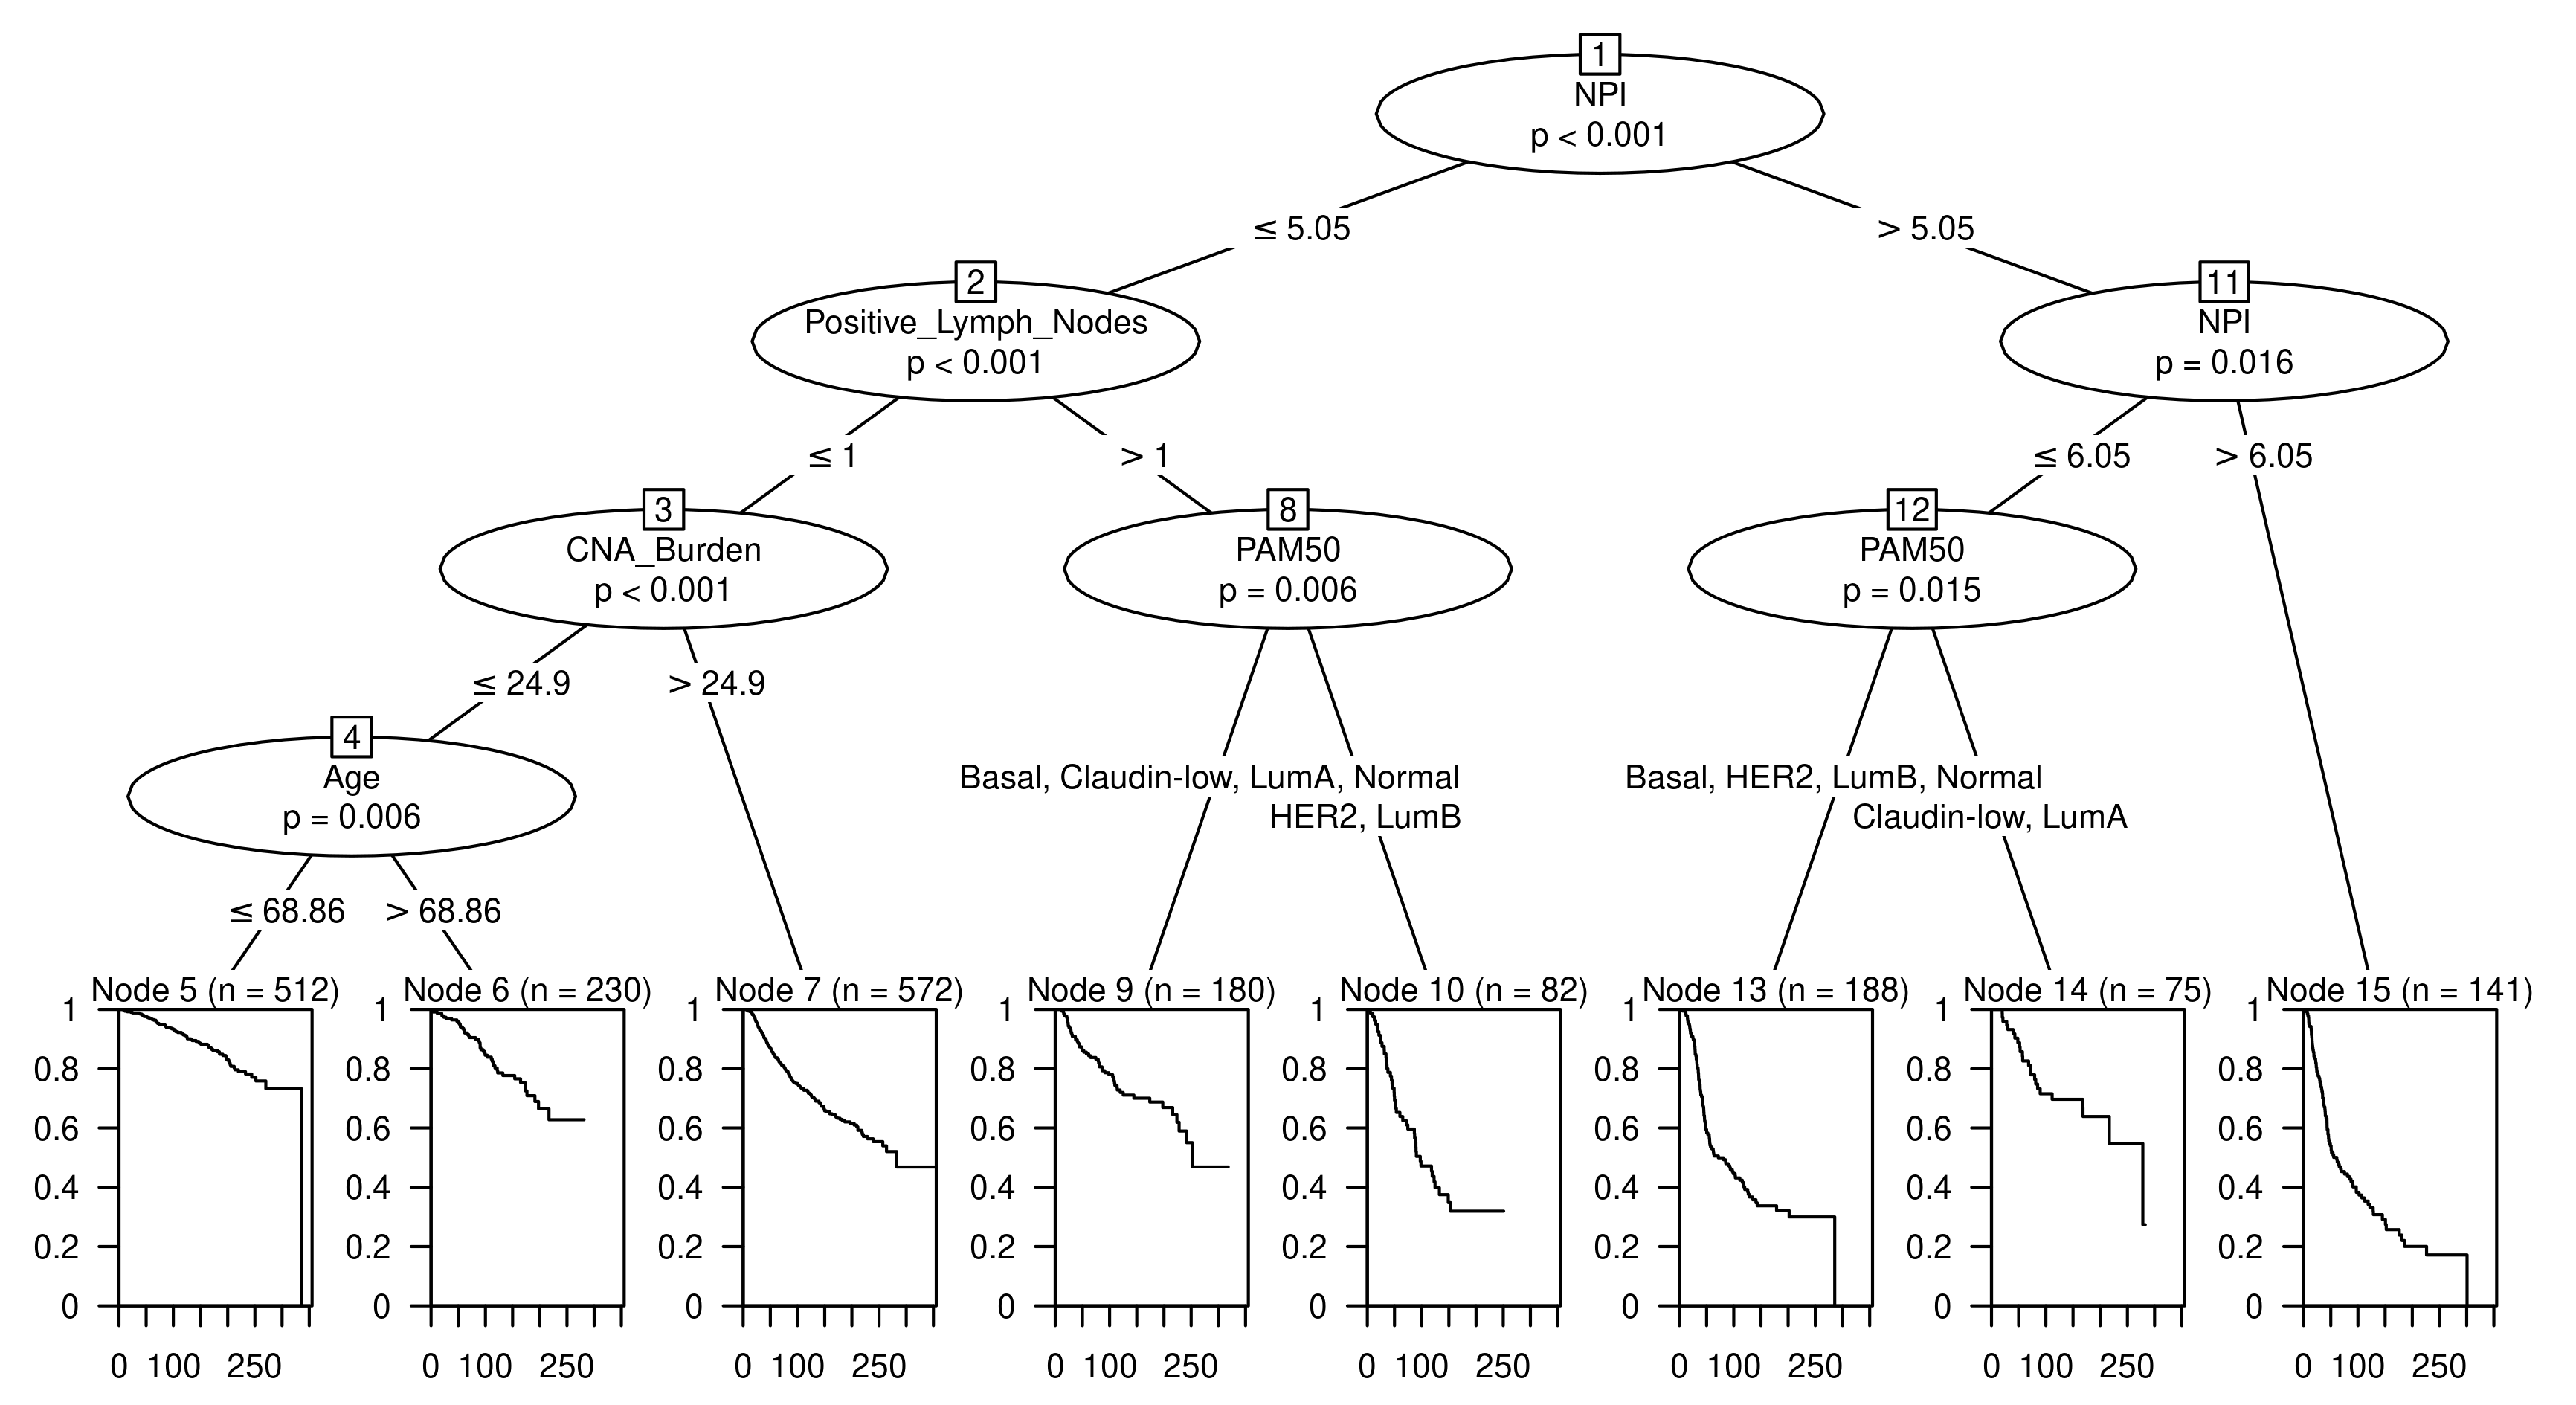
\includegraphics[width=1\textwidth]{../figures/Chapter_3/Clin_Ctree_Survival_Burden_DSS_PAM50.png}
\end{subfigure}

\vspace{1cm}

\caption[Recursive partitioning survival trees for disease-specific survival using PAM50 subtype, the six CNA Burden metrics and a number of clinical variables as candidate predictors.]{Recursive partitioning survival trees for disease-specific survival using PAM50 subtype, the six CNA Burden metrics and a number of clinical variables as candidate predictors. (A) Trees fitted using the rpart algorithm and (B) trees fitted using the ctree algorithm.}
\label{fig:PAM50_CNA_Burden_DSS_Clin}
\end{figure}

\begin{figure}[!h]
\centering

\vspace{1cm}

\begin{subfigure}{\textwidth}
\subcaption{}
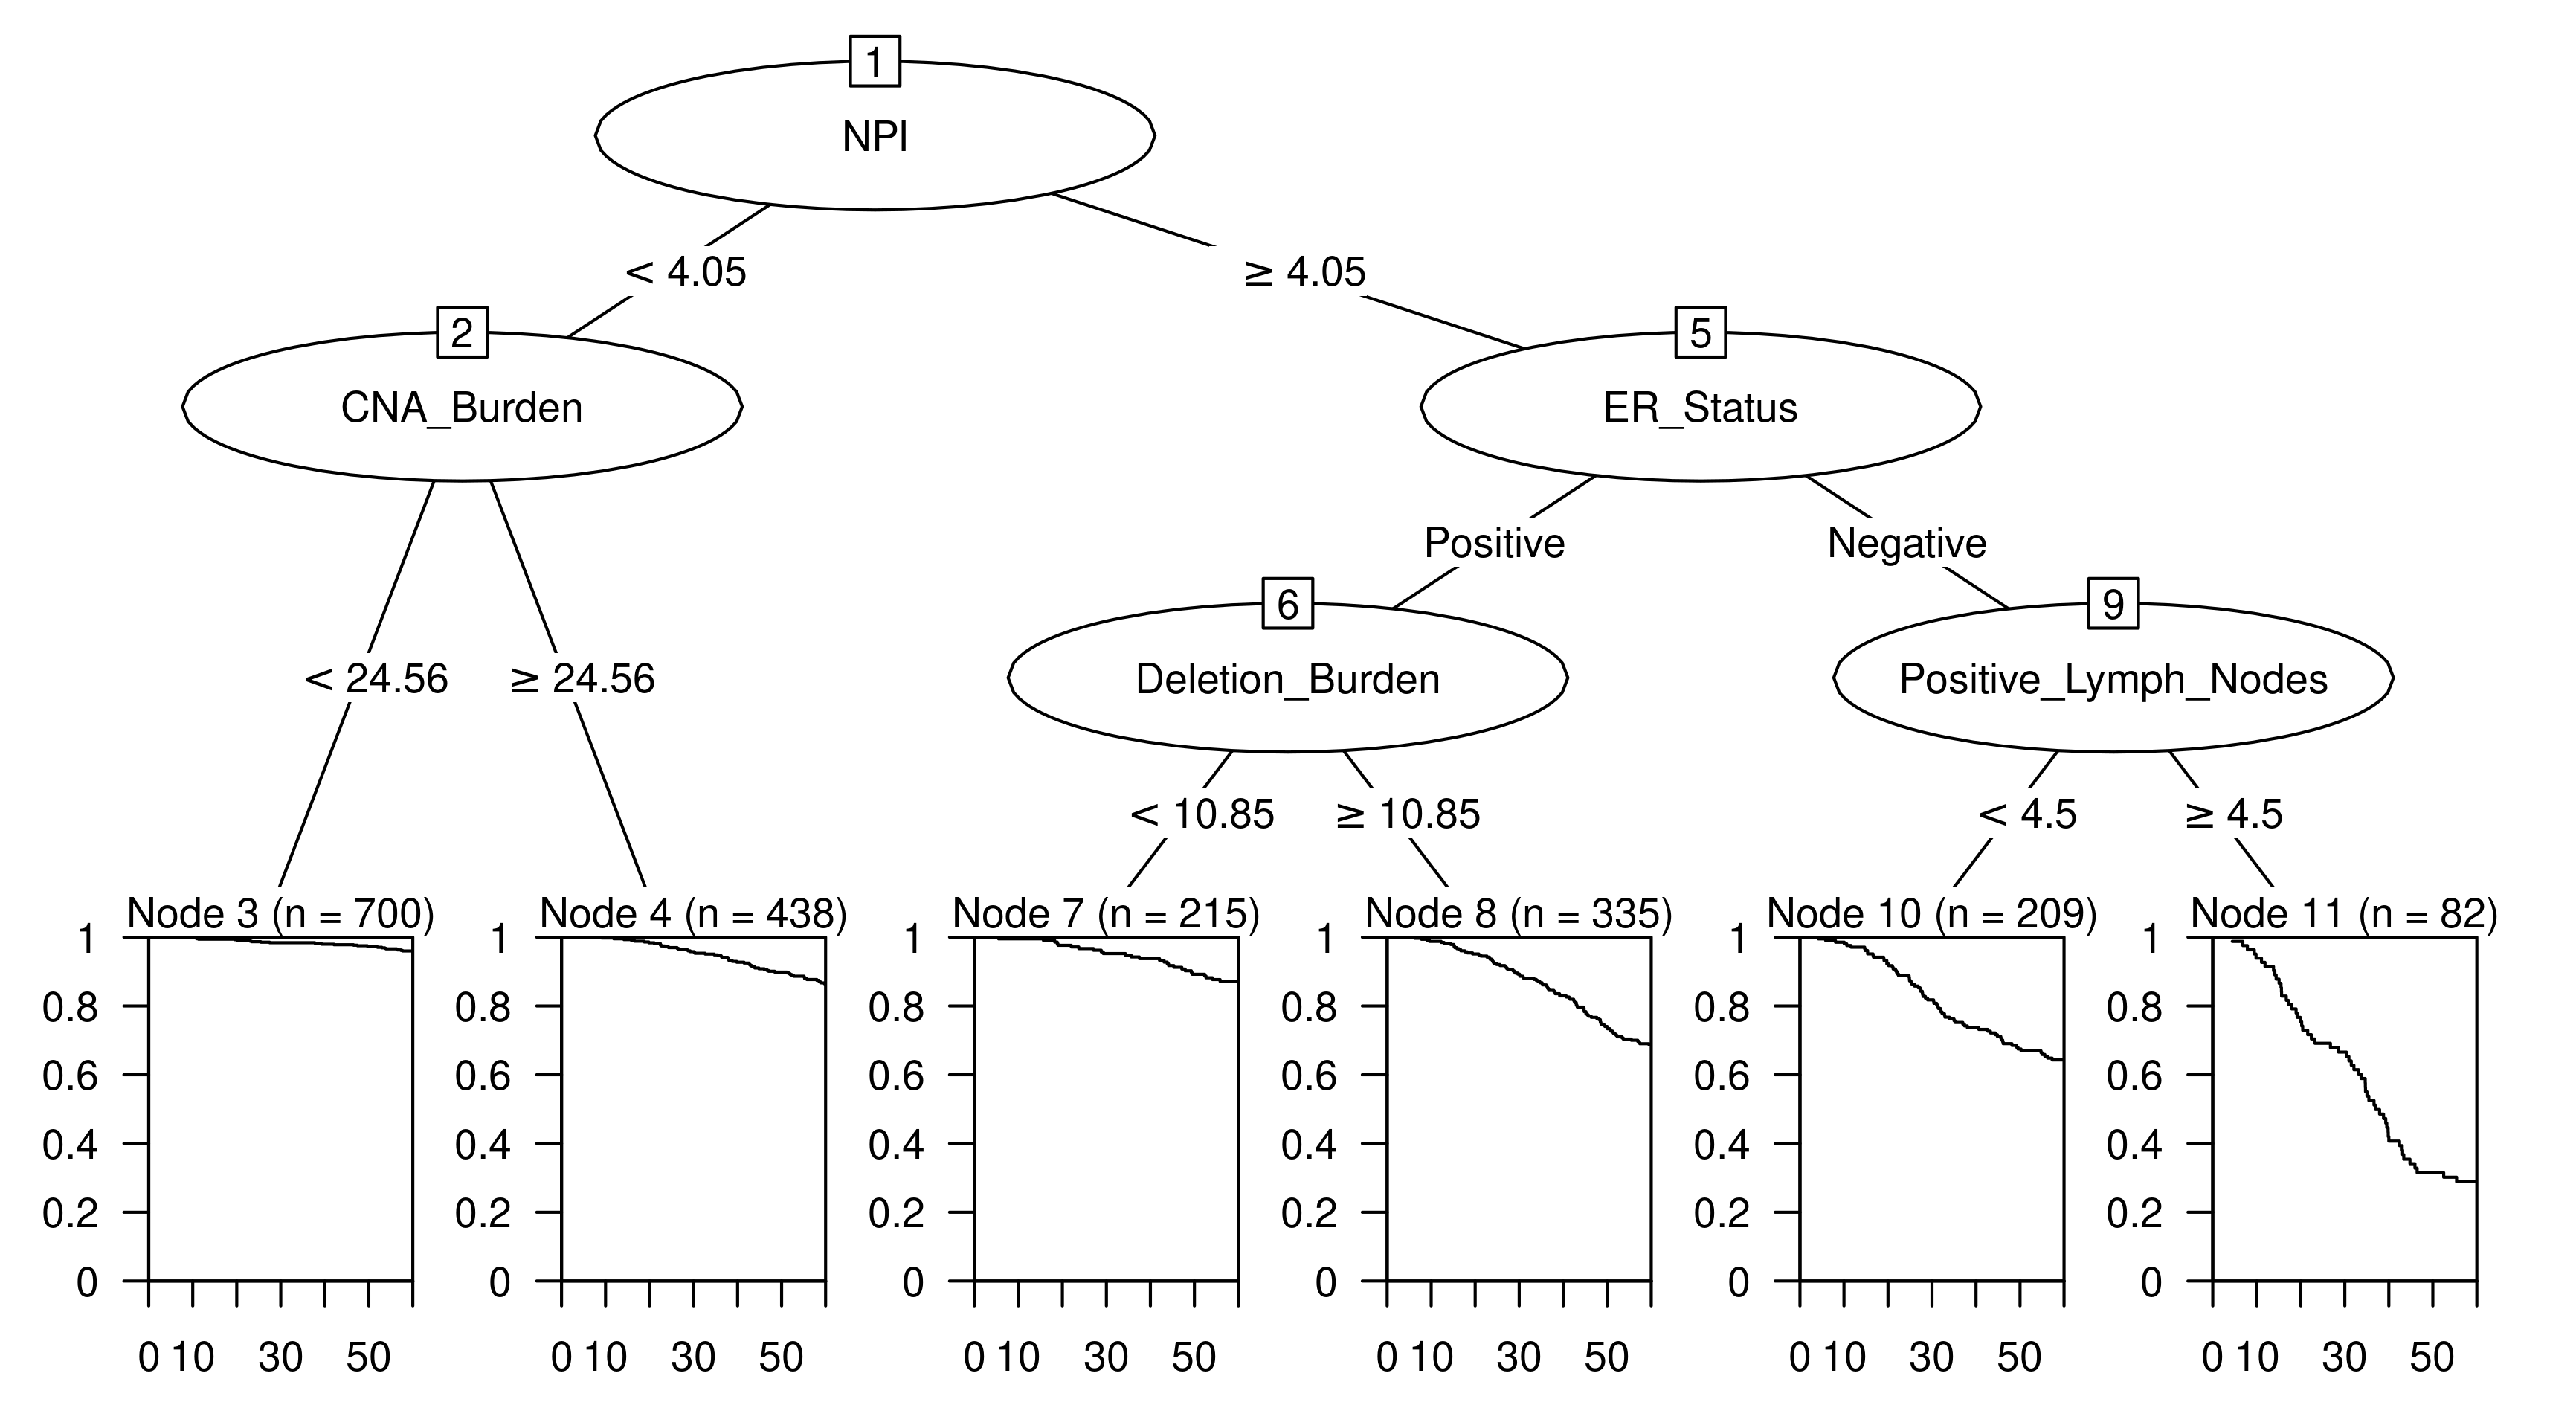
\includegraphics[width=1\textwidth]{../figures/Chapter_3/Clin_PartyKit_Survival_Burden_FiveYearDSS_PAM50.png}
\end{subfigure}

\vspace{3cm}

\begin{subfigure}{\textwidth}
\subcaption{}
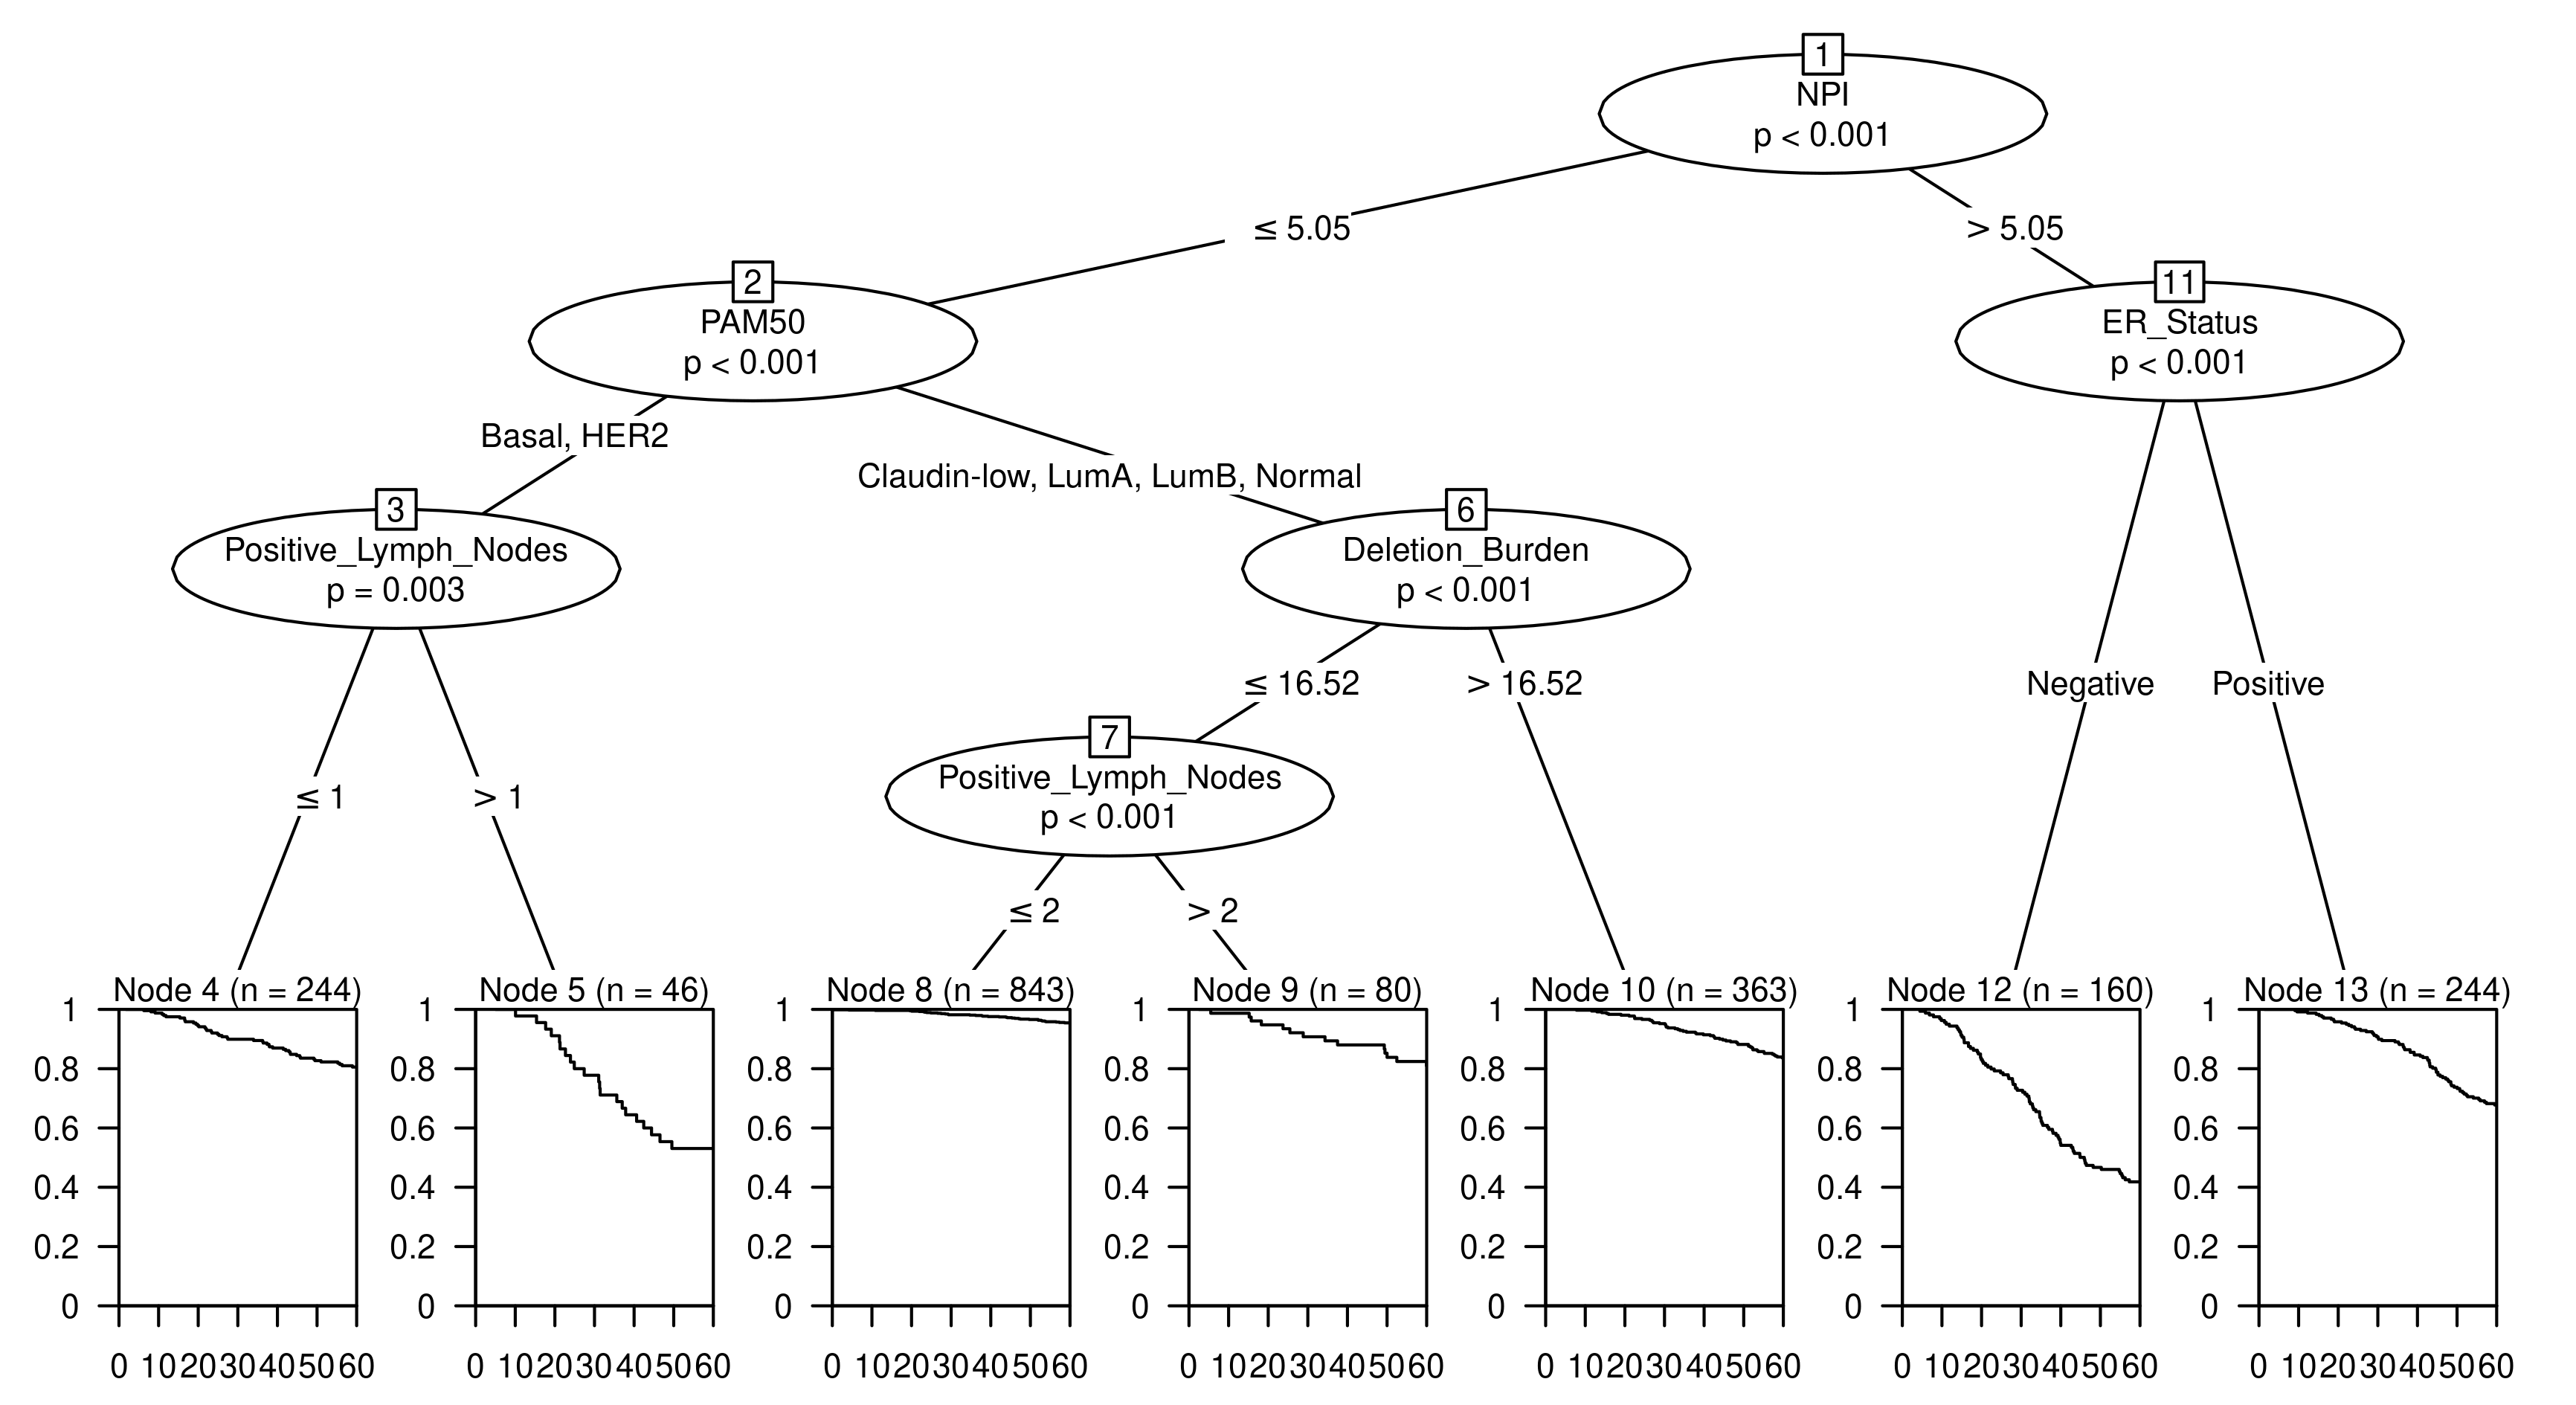
\includegraphics[width=1\textwidth]{../figures/Chapter_3/Clin_Ctree_Survival_Burden_FiveYearDSS_PAM50.png}
\end{subfigure}

\vspace{1cm}

\caption[Recursive partitioning survival trees for five-year disease-specific survival using PAM50 subtype, the six CNA Burden metrics and a number of clinical variables as candidate predictors.]{Recursive partitioning survival trees for five-year disease-specific survival using PAM50 subtype, the six CNA Burden metrics and a number of clinical variables as candidate predictors. (A) Trees fitted using the rpart algorithm and (B) trees fitted using the ctree algorithm.}
\label{fig:PAM50_CNA_Burden_FiveYearDSS_Clin}
\end{figure}

\begin{figure}[!h]
\centering

\vspace{1cm}

\begin{subfigure}{\textwidth}
\subcaption{}
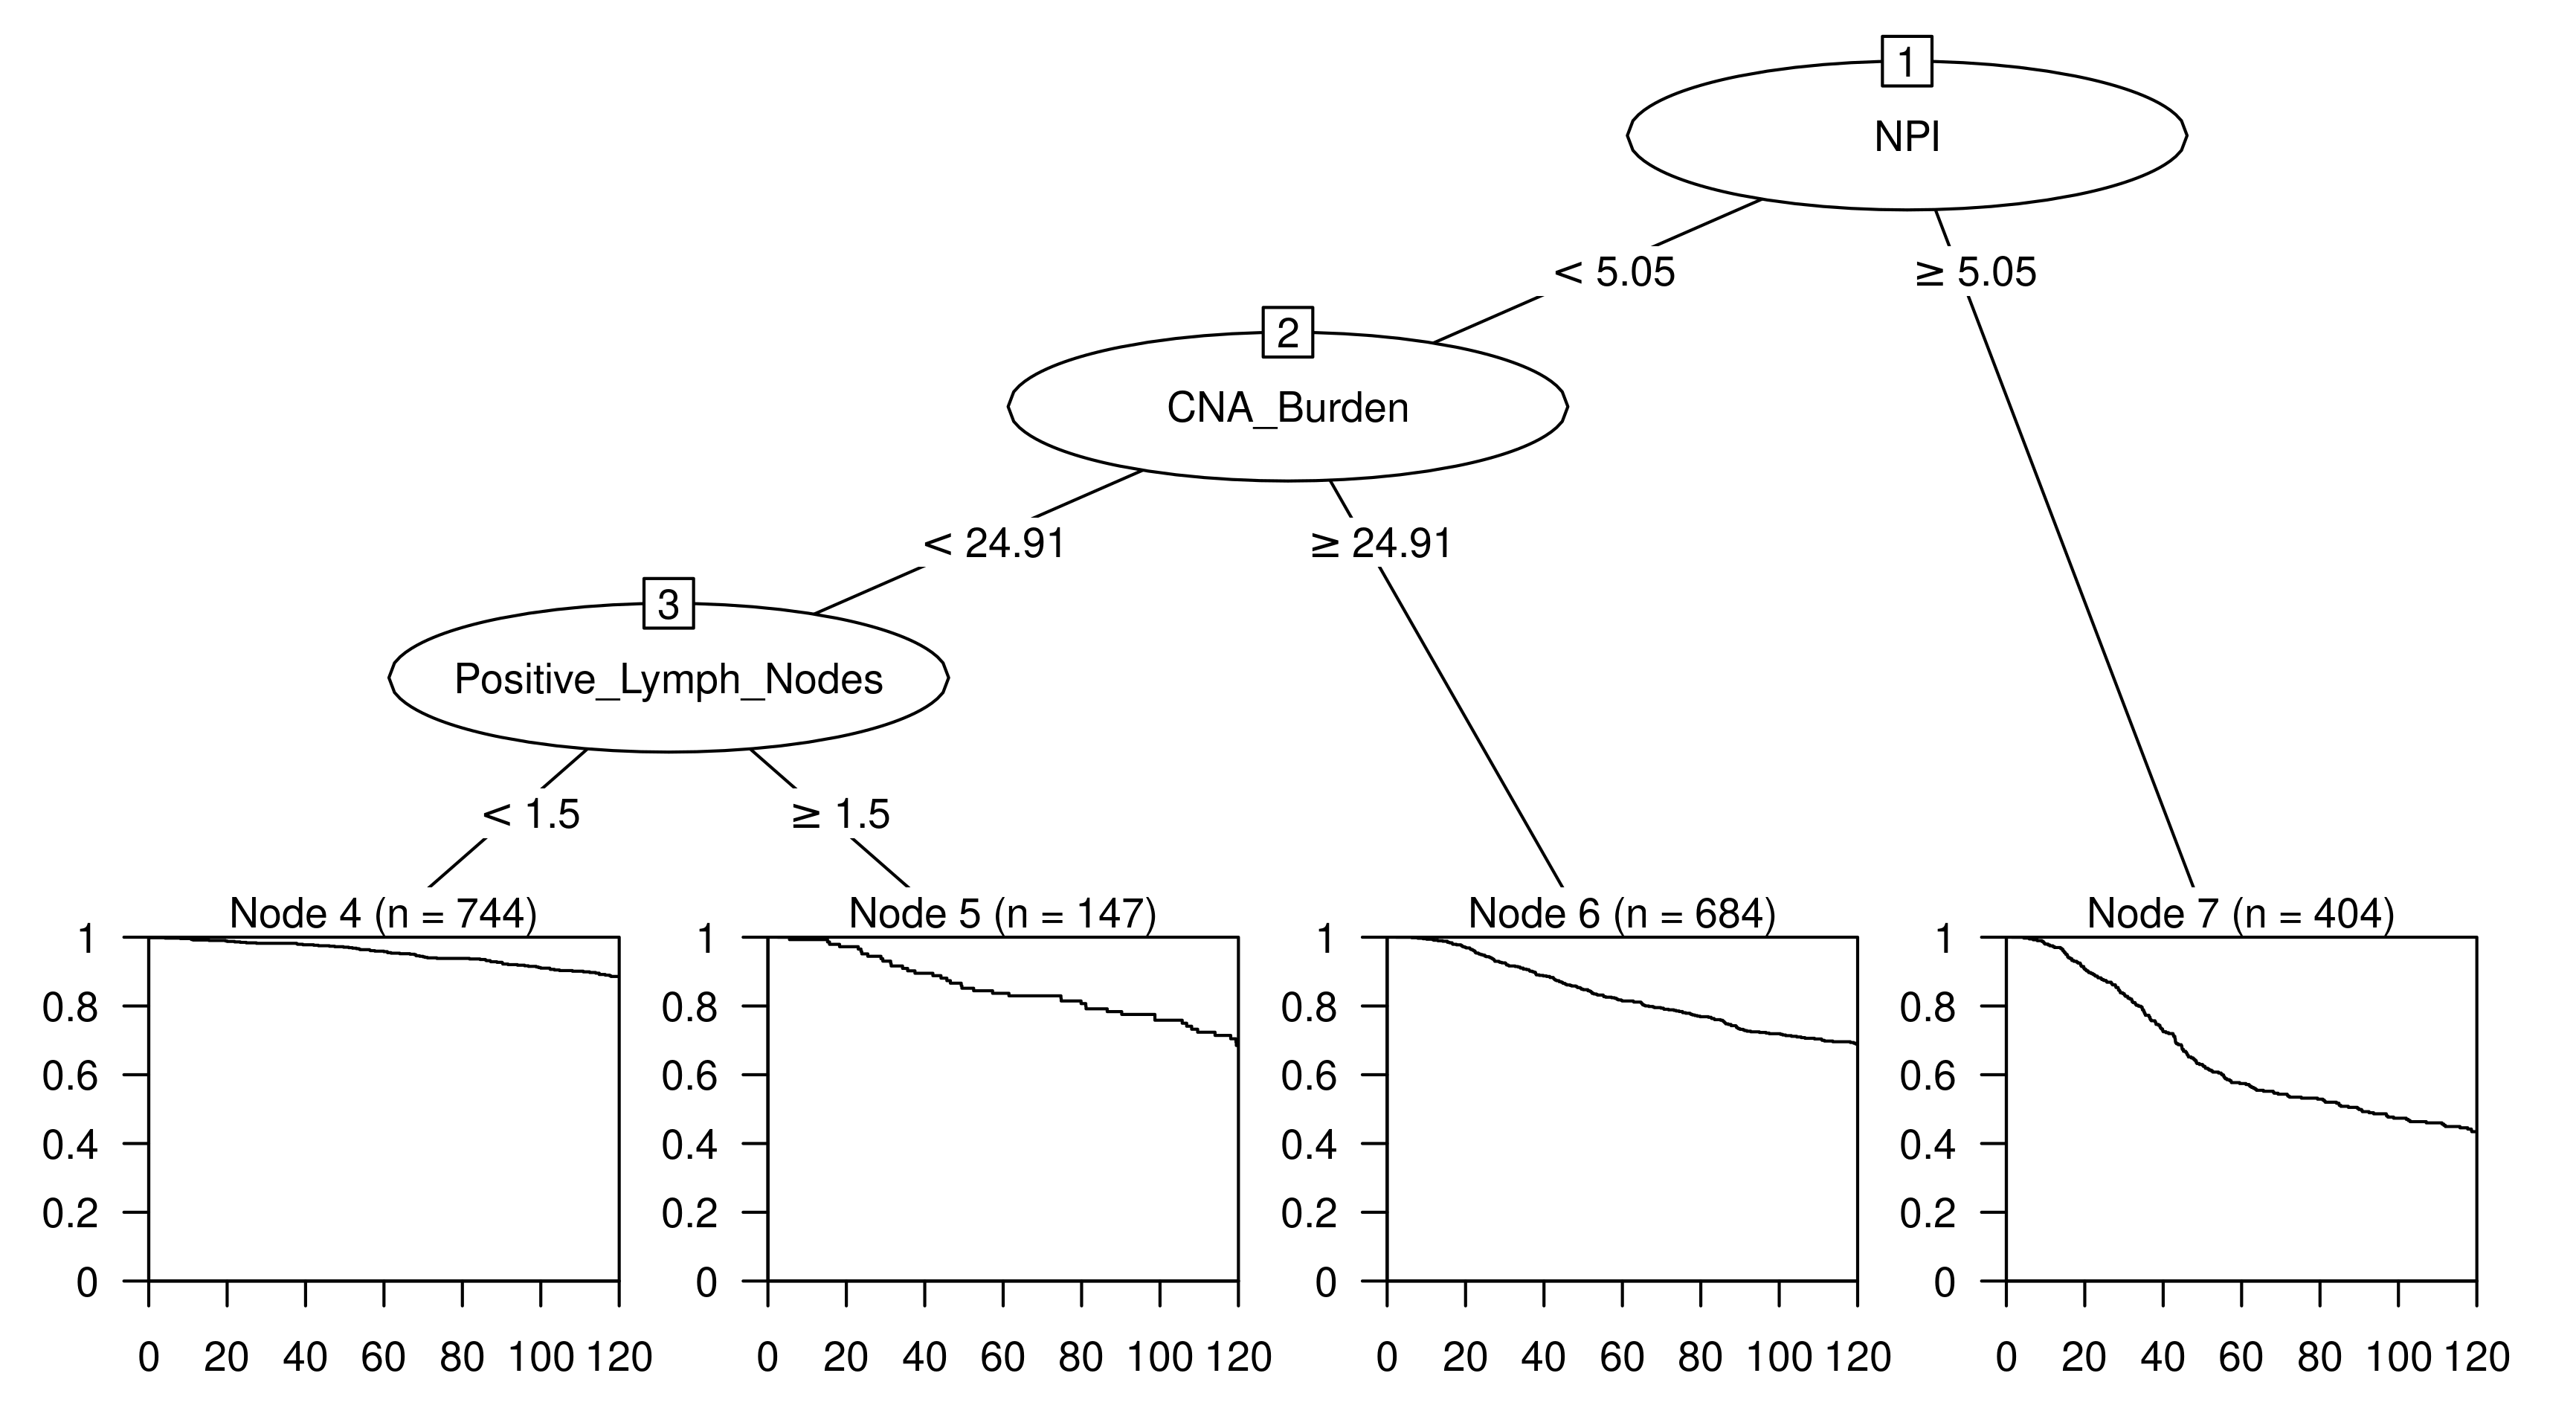
\includegraphics[width=1\textwidth]{../figures/Chapter_3/Clin_PartyKit_Survival_Burden_TenYearDSS_PAM50.png}
\end{subfigure}

\vspace{3cm}

\begin{subfigure}{\textwidth}
\subcaption{}
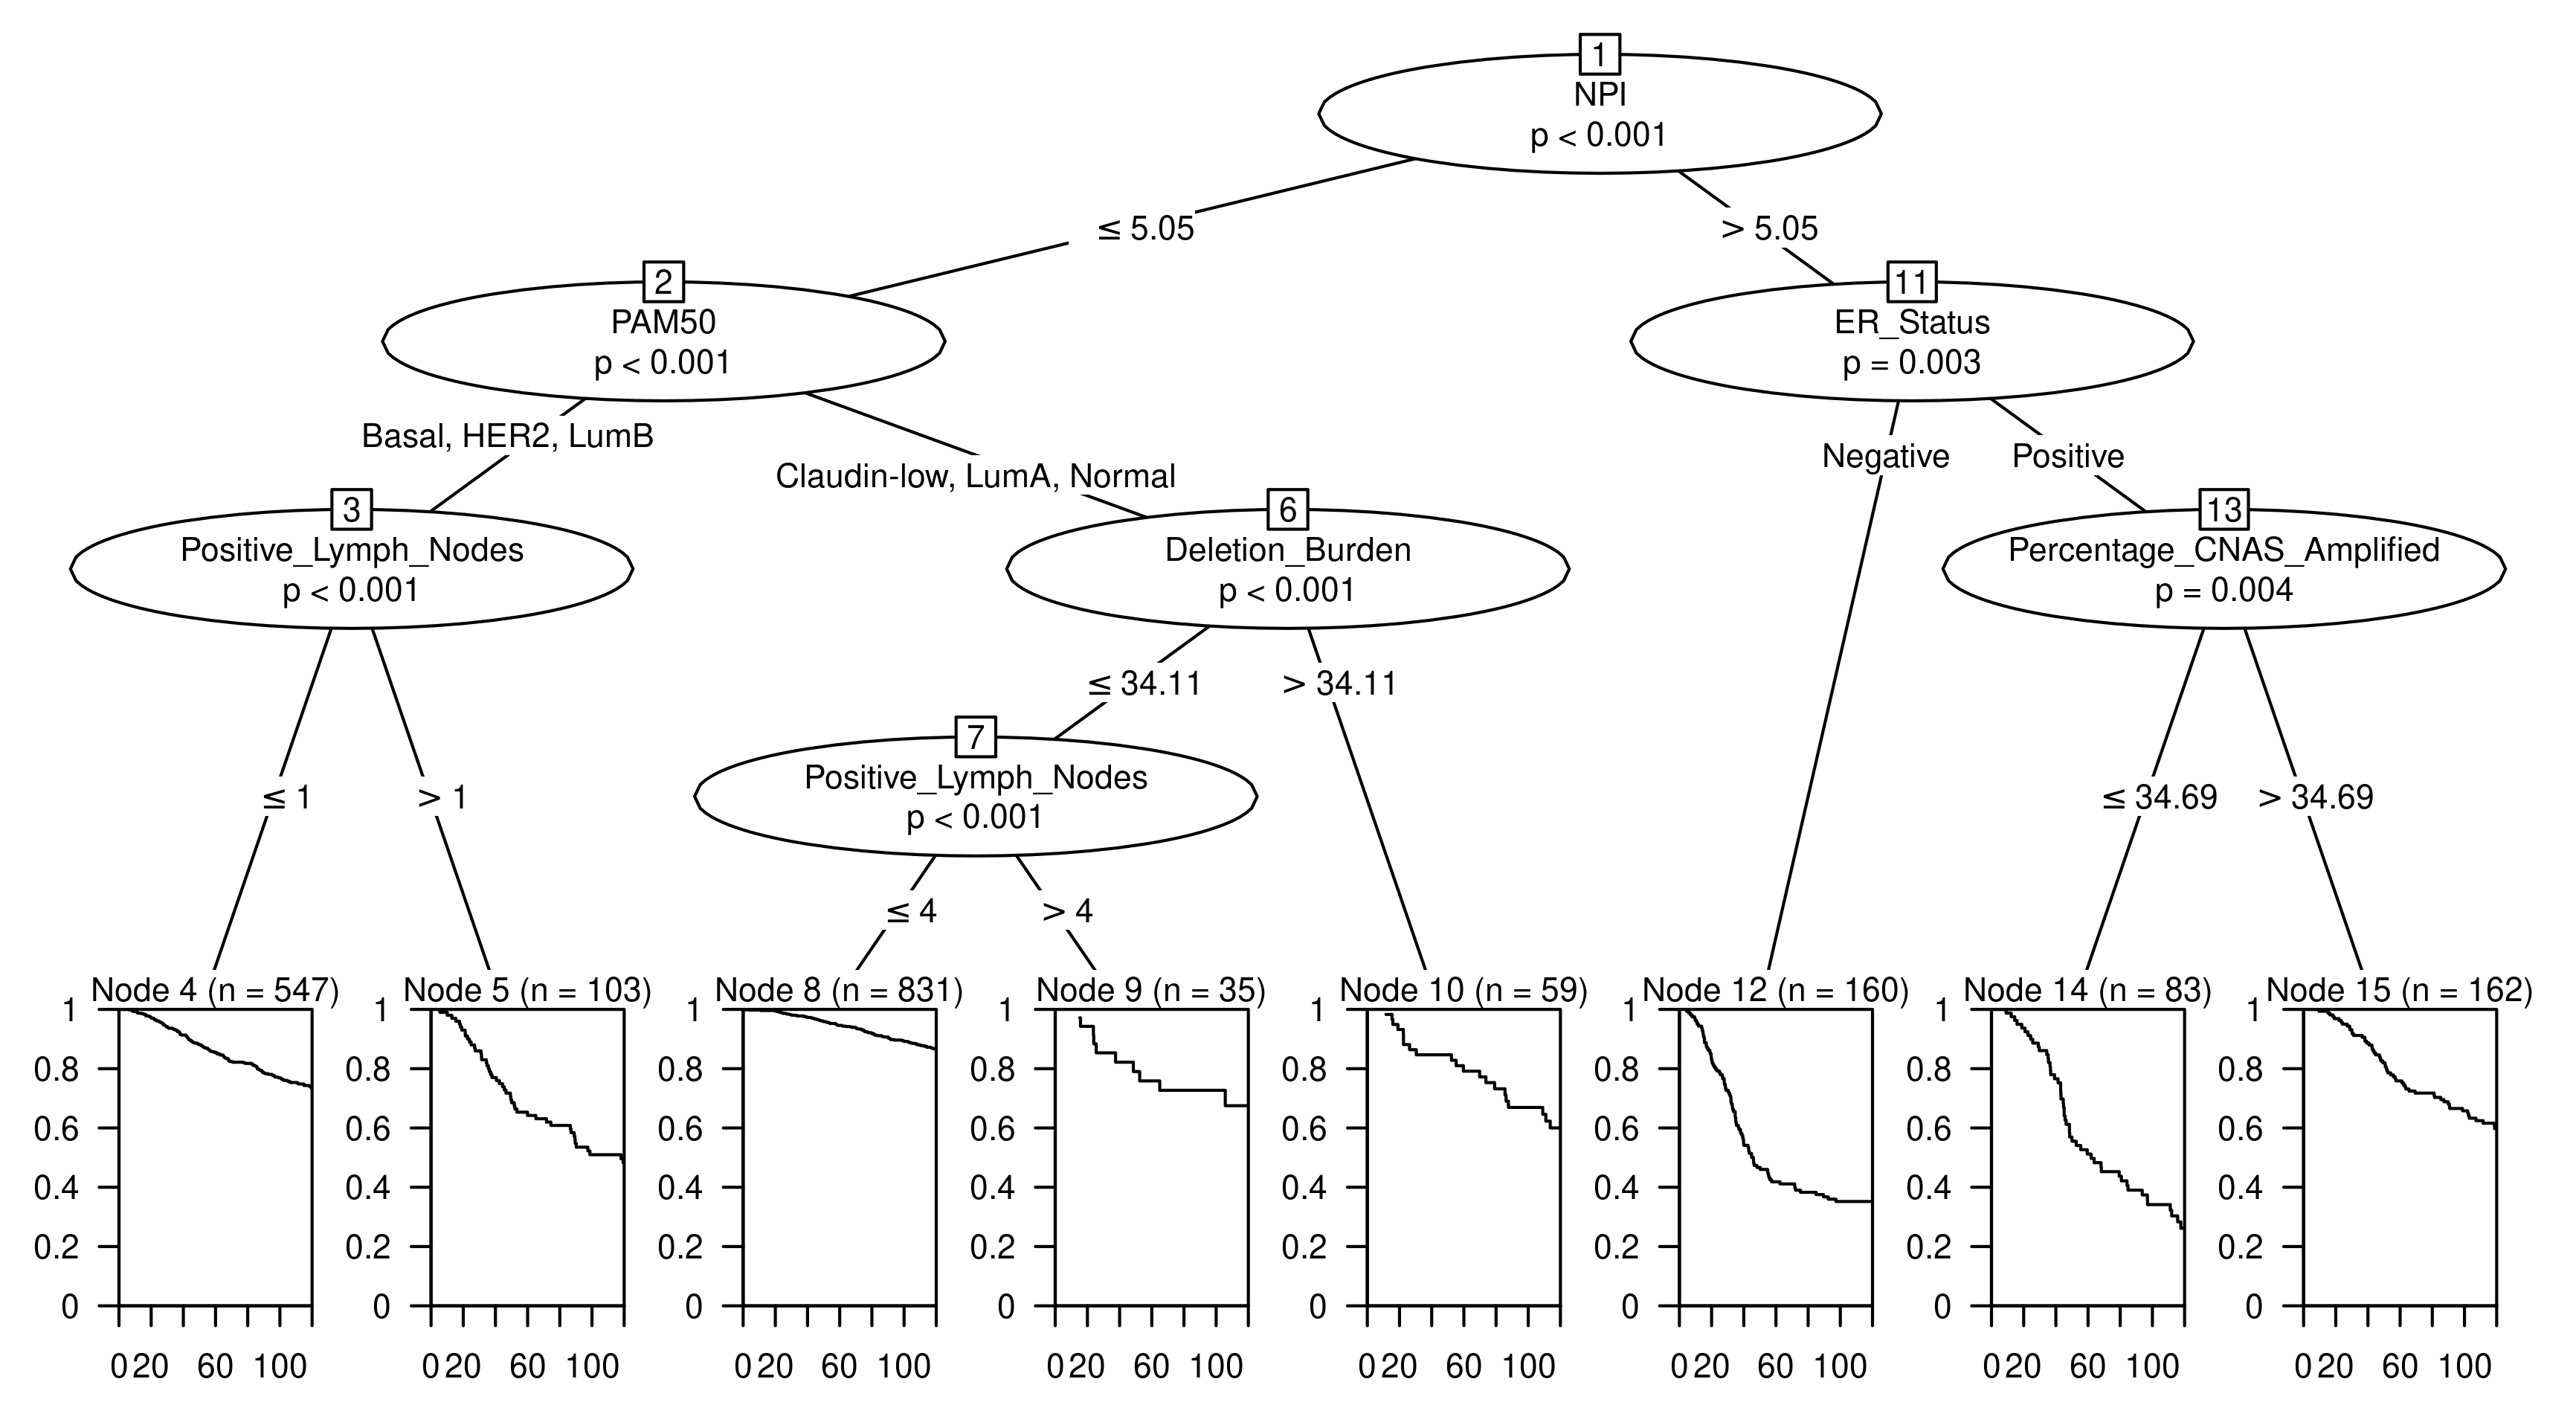
\includegraphics[width=1\textwidth]{../figures/Chapter_3/Clin_Ctree_Survival_Burden_TenYearDSS_PAM50.png}
\end{subfigure}

\vspace{1cm}

\caption[Recursive partitioning survival trees for ten-year disease-specific survival using PAM50 subtype, the six CNA Burden metrics and a number of clinical variables as candidate predictors.]{Recursive partitioning survival trees for ten-year disease-specific survival using PAM50 subtype, the six CNA Burden metrics and a number of clinical variables as candidate predictors. (A) Trees fitted using the rpart algorithm and (B) trees fitted using the ctree algorithm.}
\label{fig:PAM50_CNA_Burden_TenYearDSS_Clin}
\end{figure}

\begin{figure}[!h]
\centering

\vspace{1cm}

\begin{subfigure}{\textwidth}
\subcaption{}
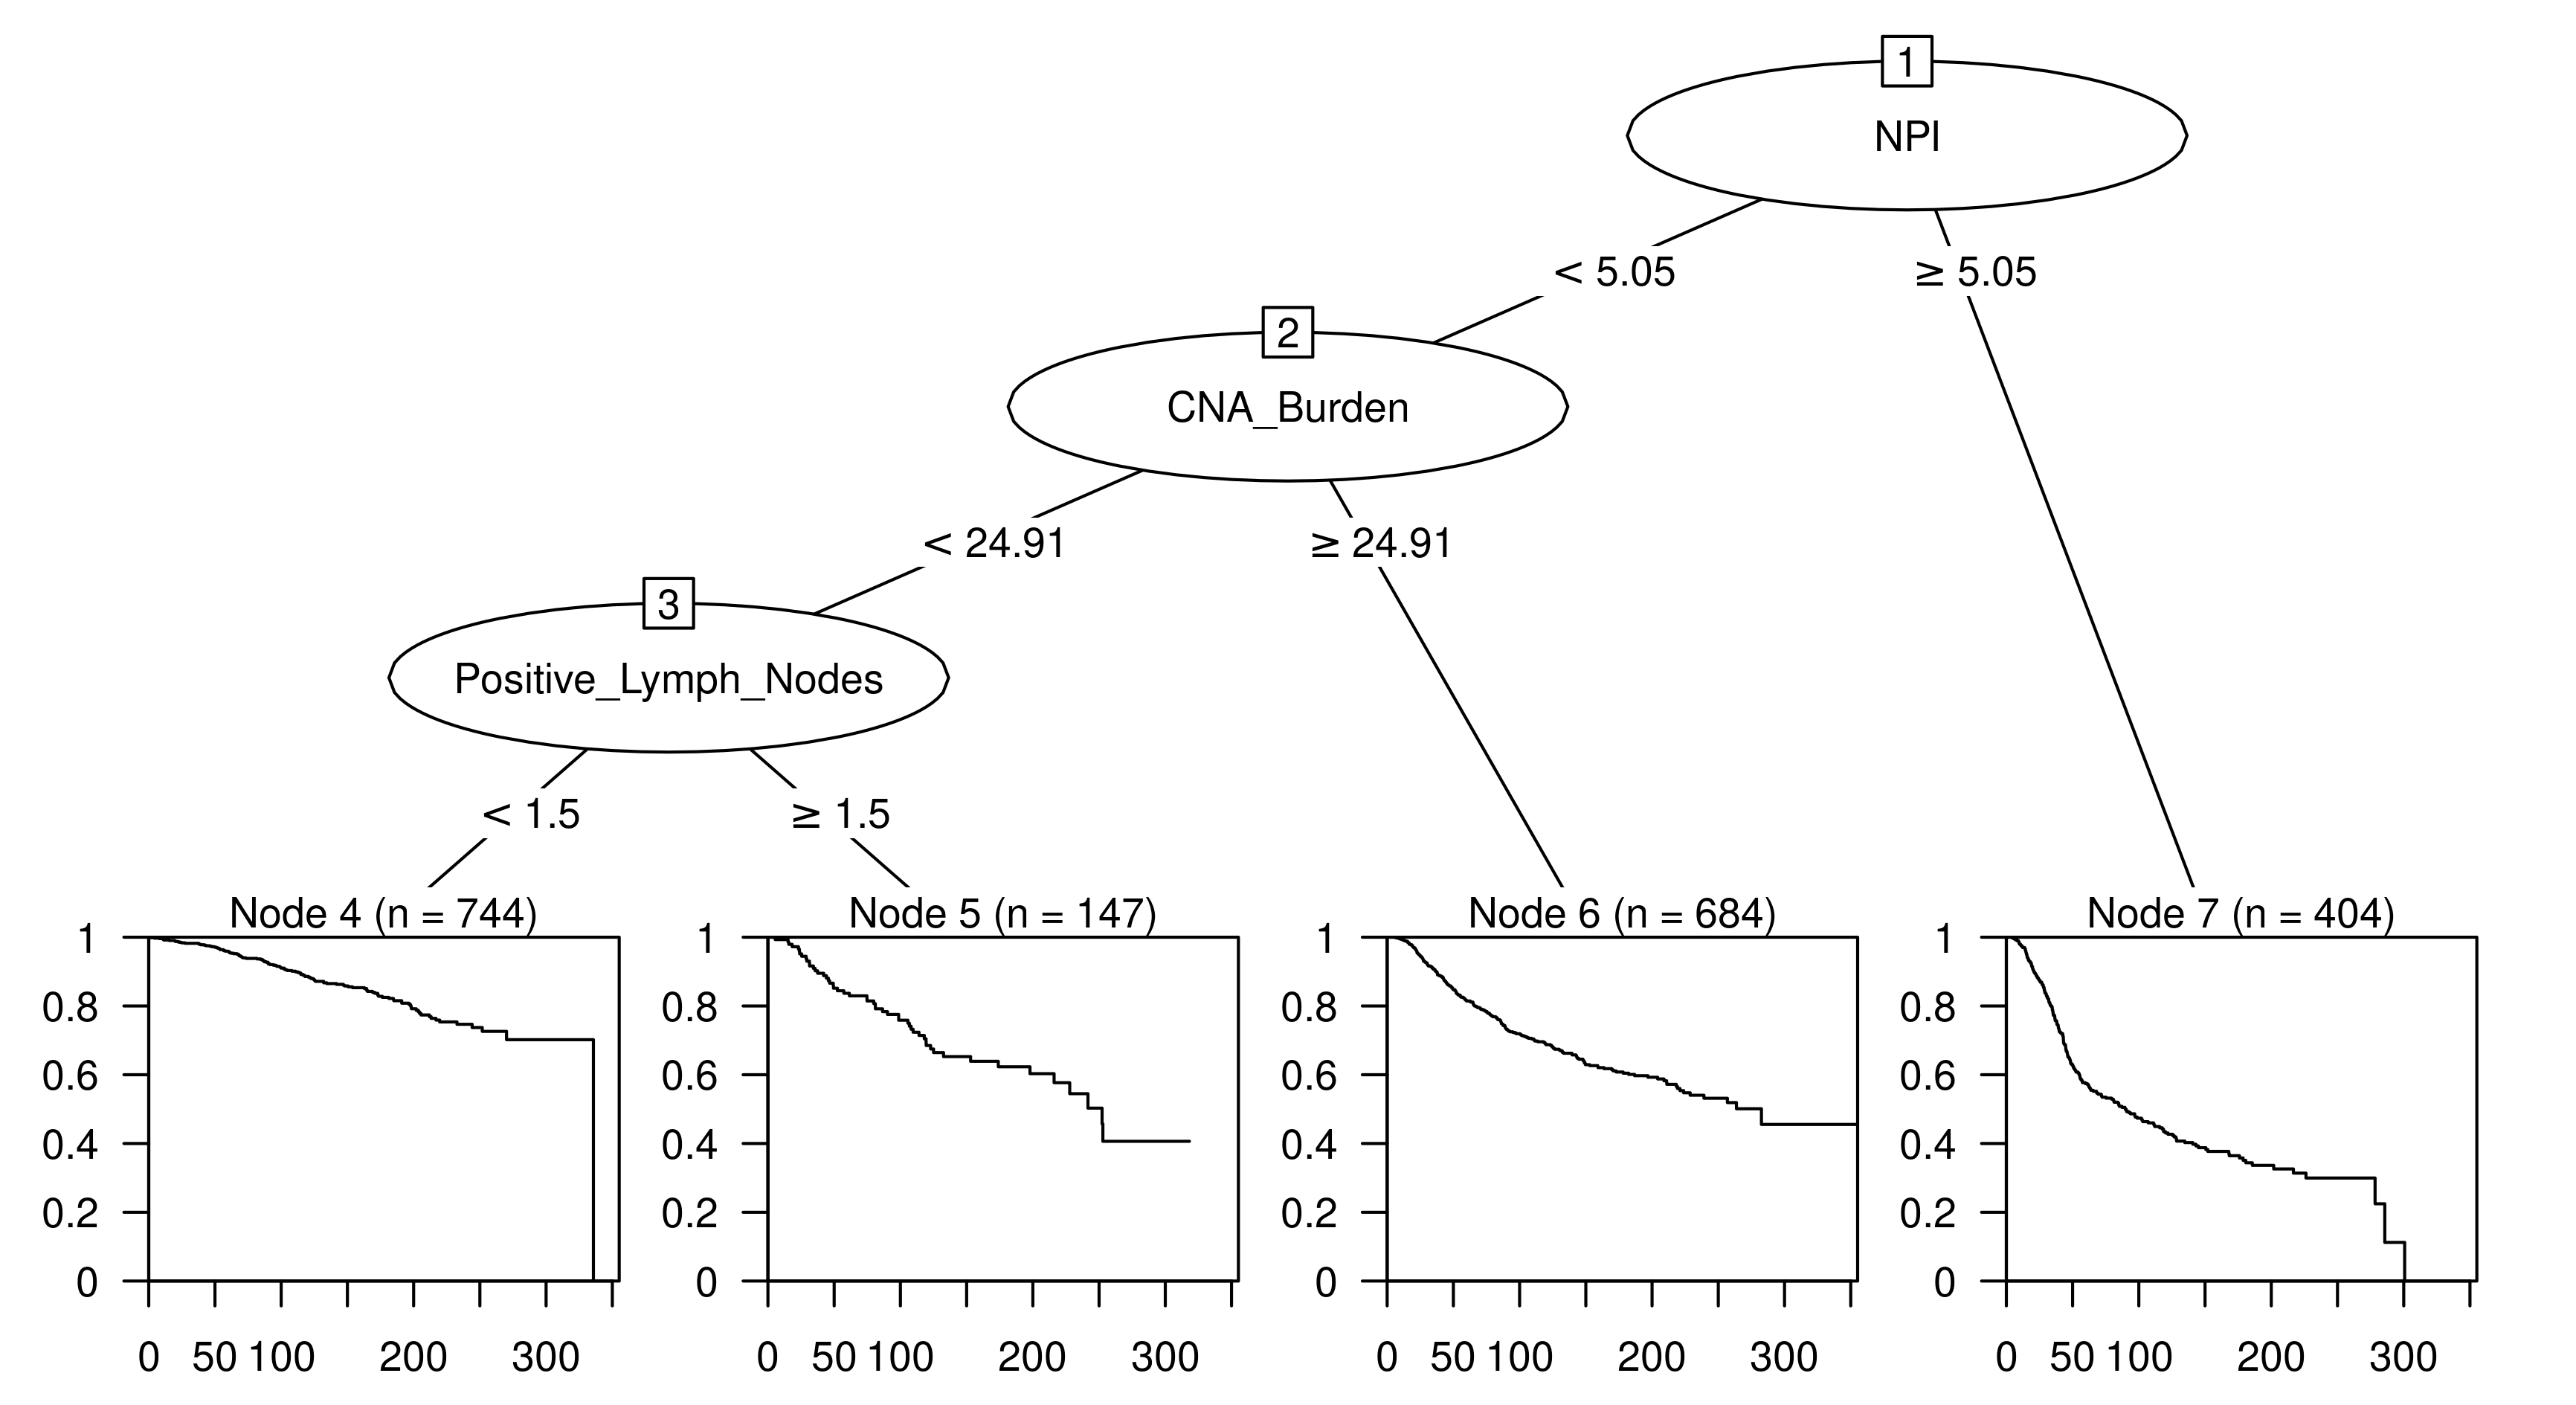
\includegraphics[width=1\textwidth]{../figures/Chapter_3/Clin_PartyKit_Survival_Burden_DSS_INTCLUST.png}
\end{subfigure}

\vspace{3cm}

\begin{subfigure}{\textwidth}
\subcaption{}
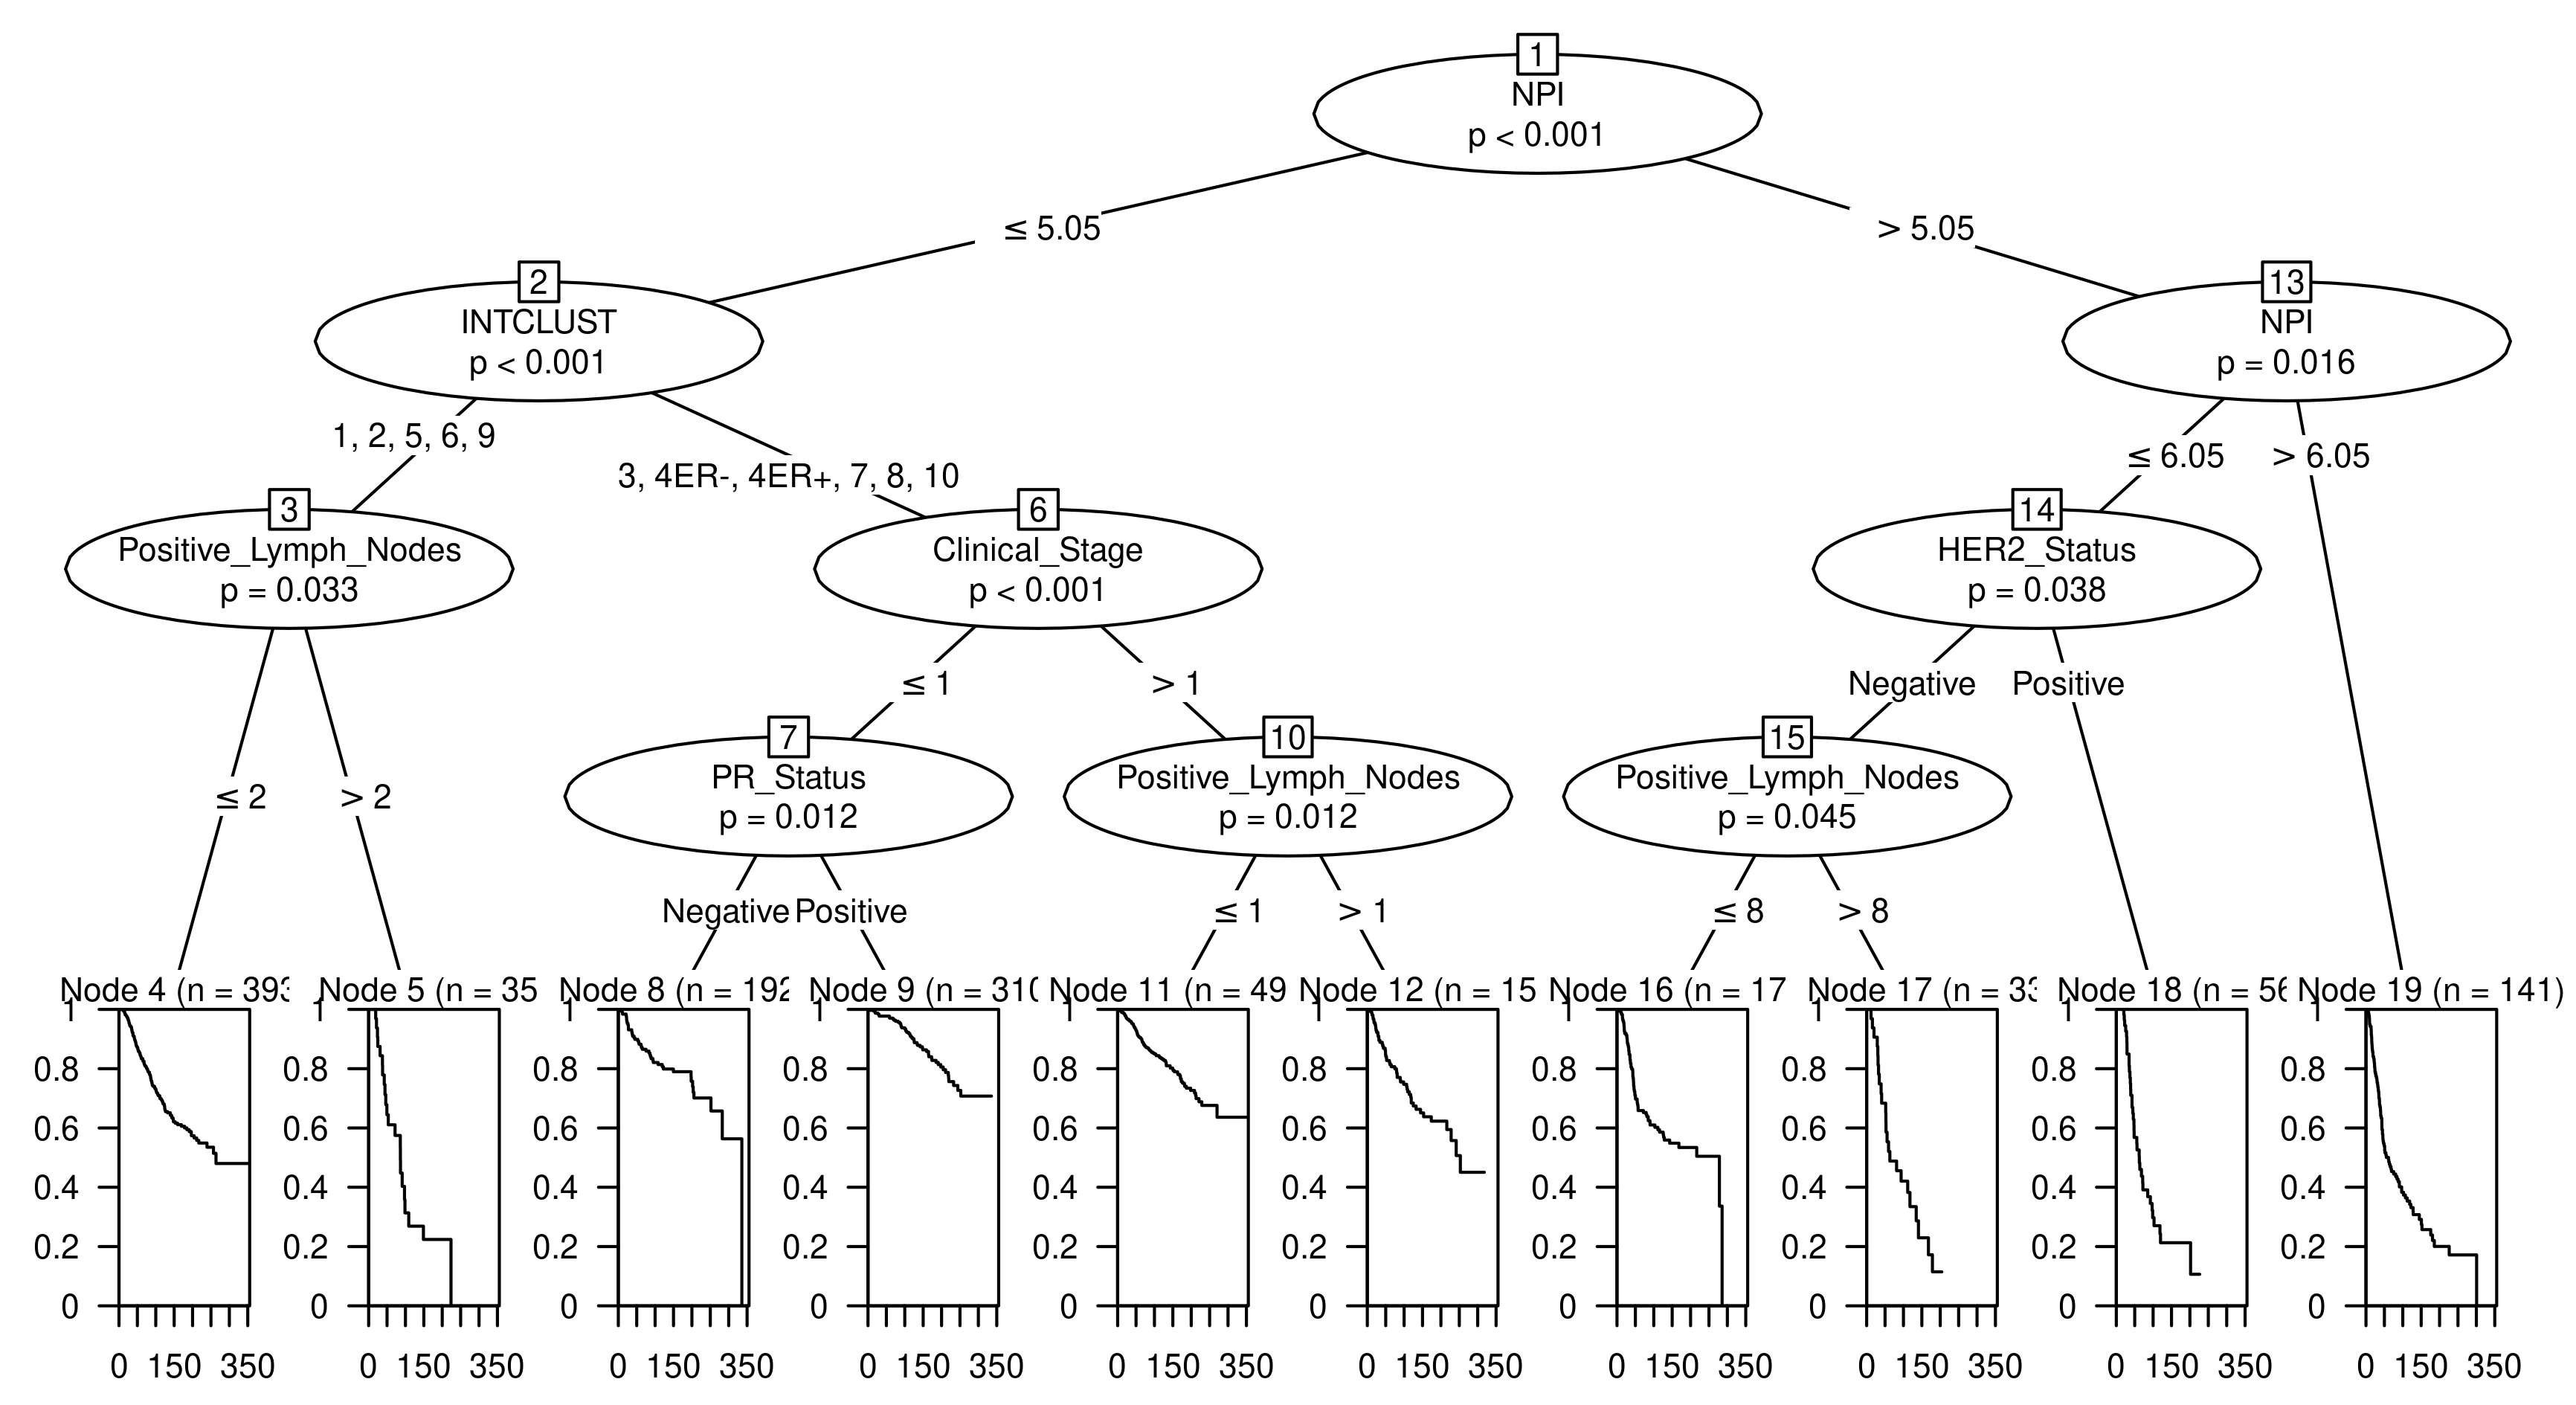
\includegraphics[width=1\textwidth]{../figures/Chapter_3/Clin_Ctree_Survival_Burden_DSS_INTCLUST.png}
\end{subfigure}

\vspace{1cm}

\caption[Recursive partitioning survival trees for disease-specific survival using Integrative Cluster the six CNA Burden metrics and a number of clinical variables as candidate predictors.]{Recursive partitioning survival trees for disease-specific survival using Integrative Cluster, the six CNA Burden metrics and a number of clinical variables as candidate predictors. (A) Trees fitted using the rpart algorithm and (B) trees fitted using the ctree algorithm.}
\label{fig:INTCLUST_CNA_Burden_DSS_Clin}
\end{figure}

\begin{figure}[!h]
\centering

\vspace{1cm}

\begin{subfigure}{\textwidth}
\subcaption{}
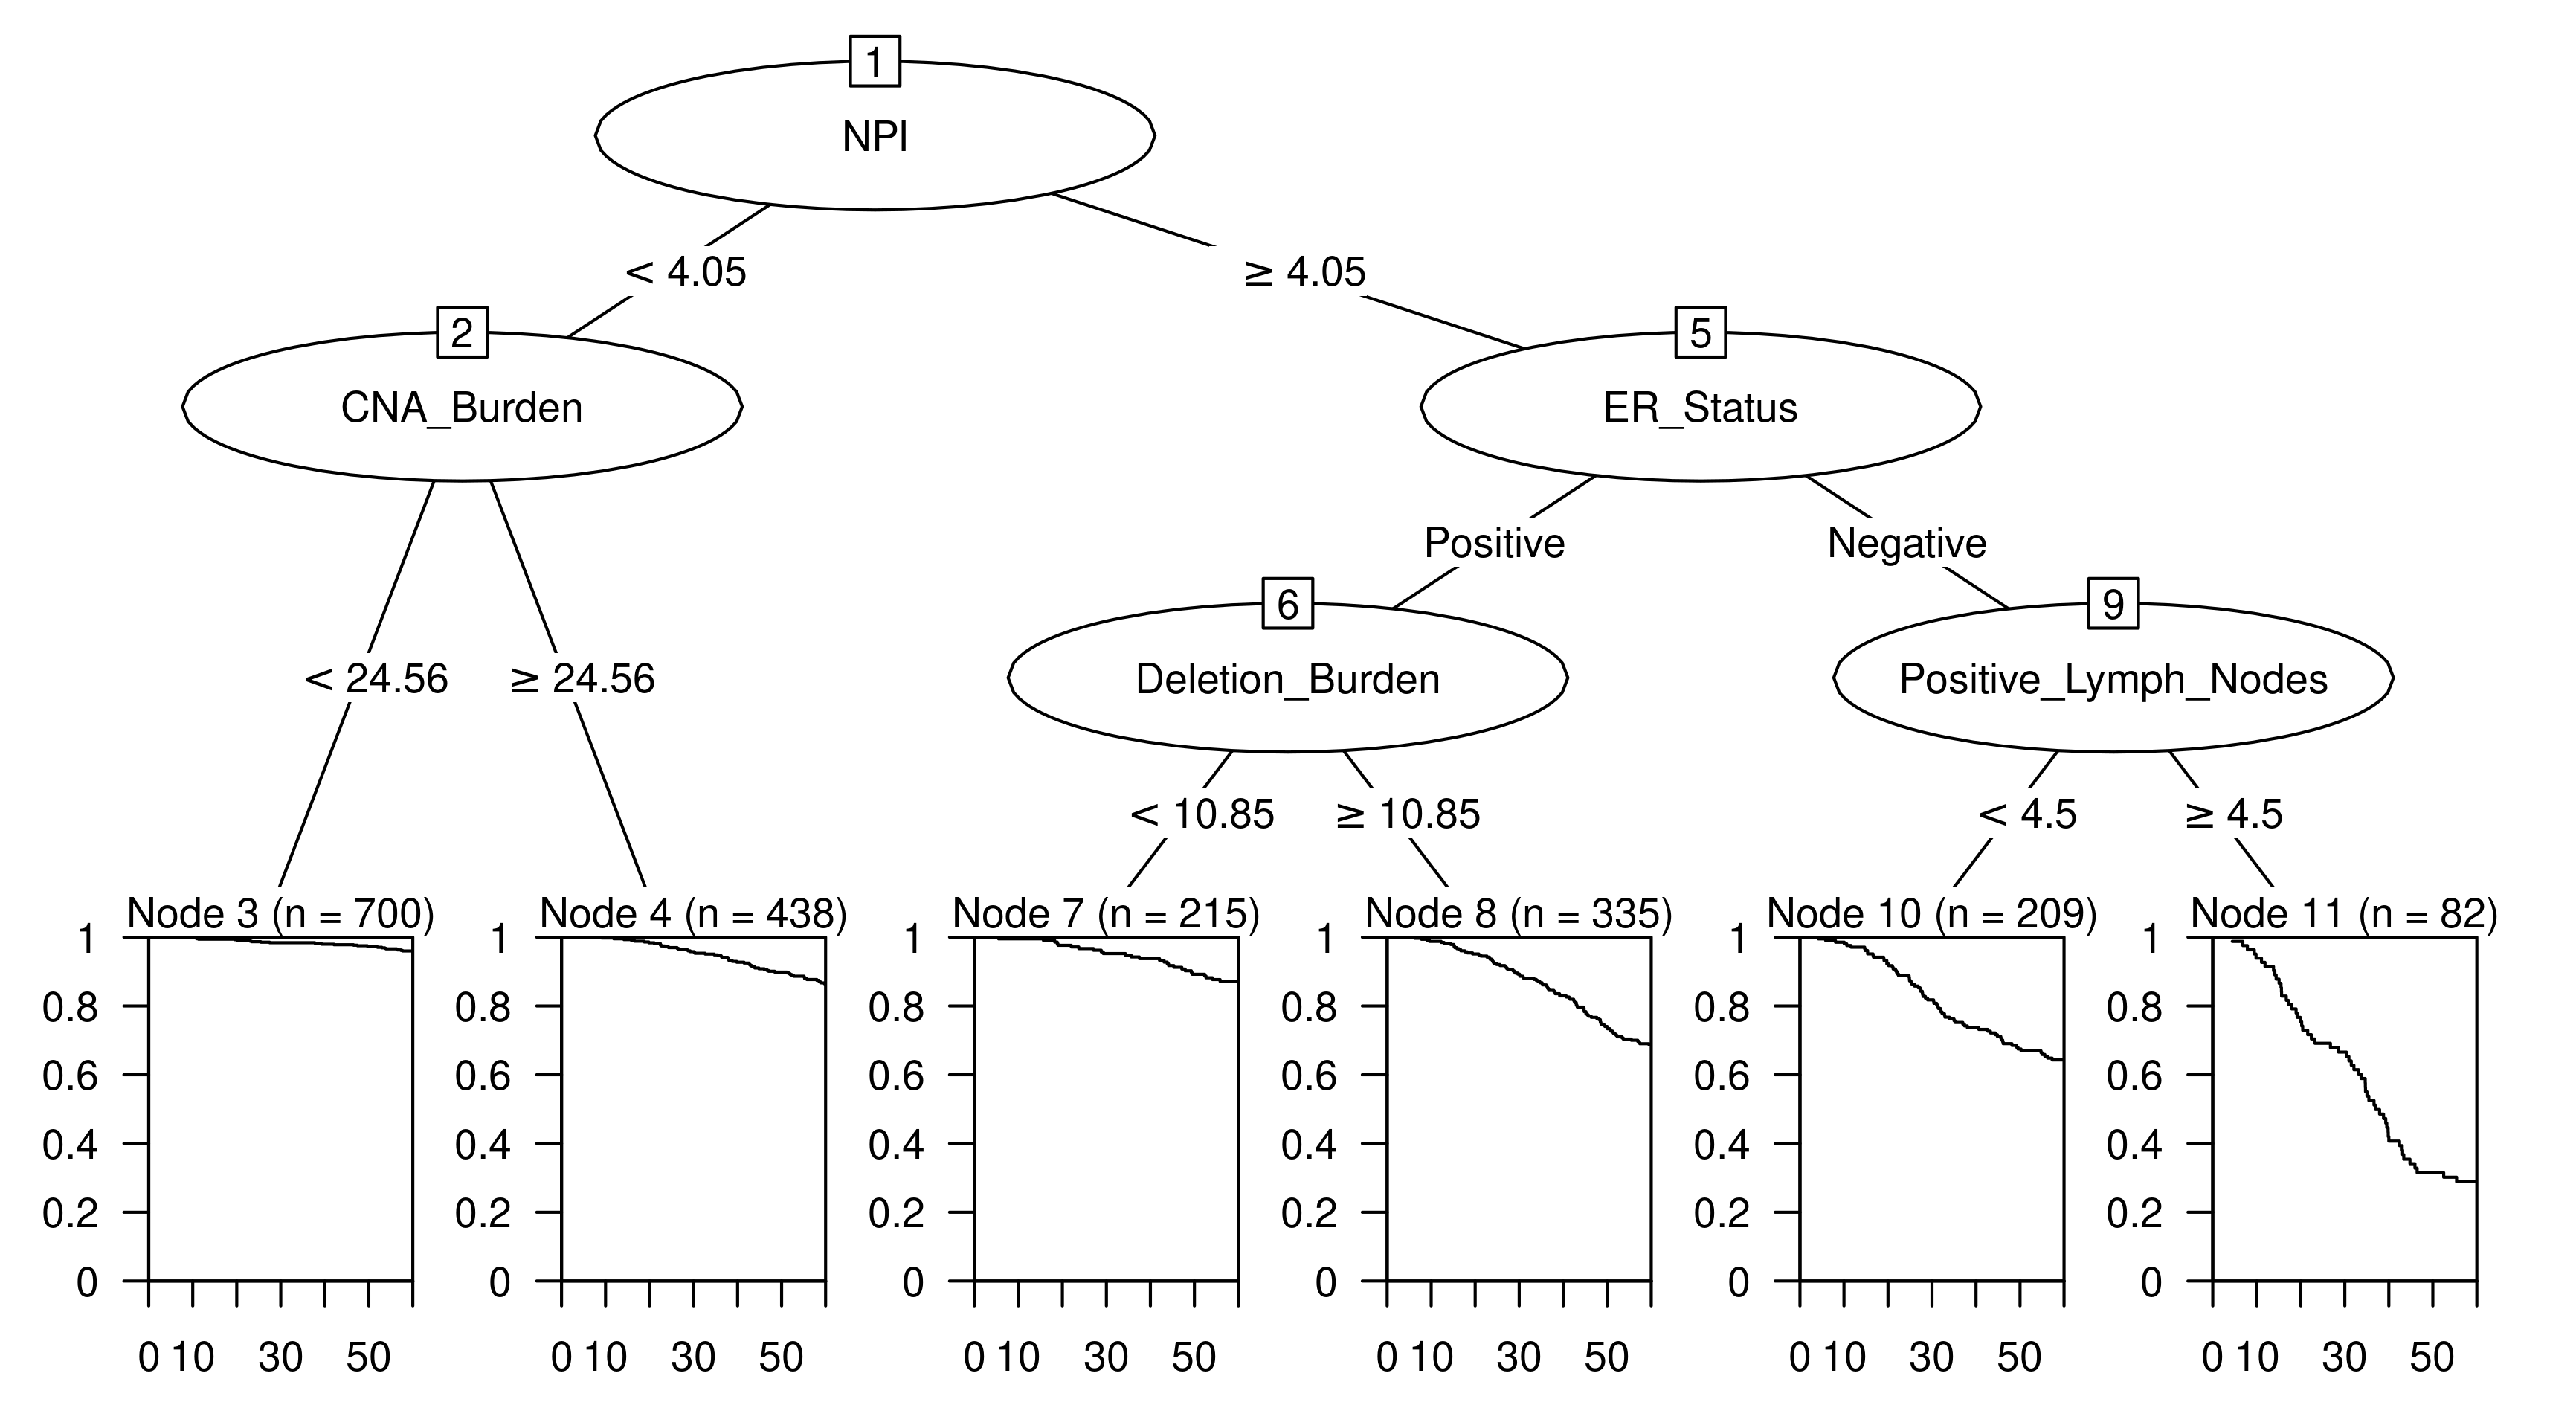
\includegraphics[width=1\textwidth]{../figures/Chapter_3/Clin_PartyKit_Survival_Burden_FiveYearDSS_INTCLUST.png}
\end{subfigure}

\vspace{3cm}

\begin{subfigure}{\textwidth}
\subcaption{}
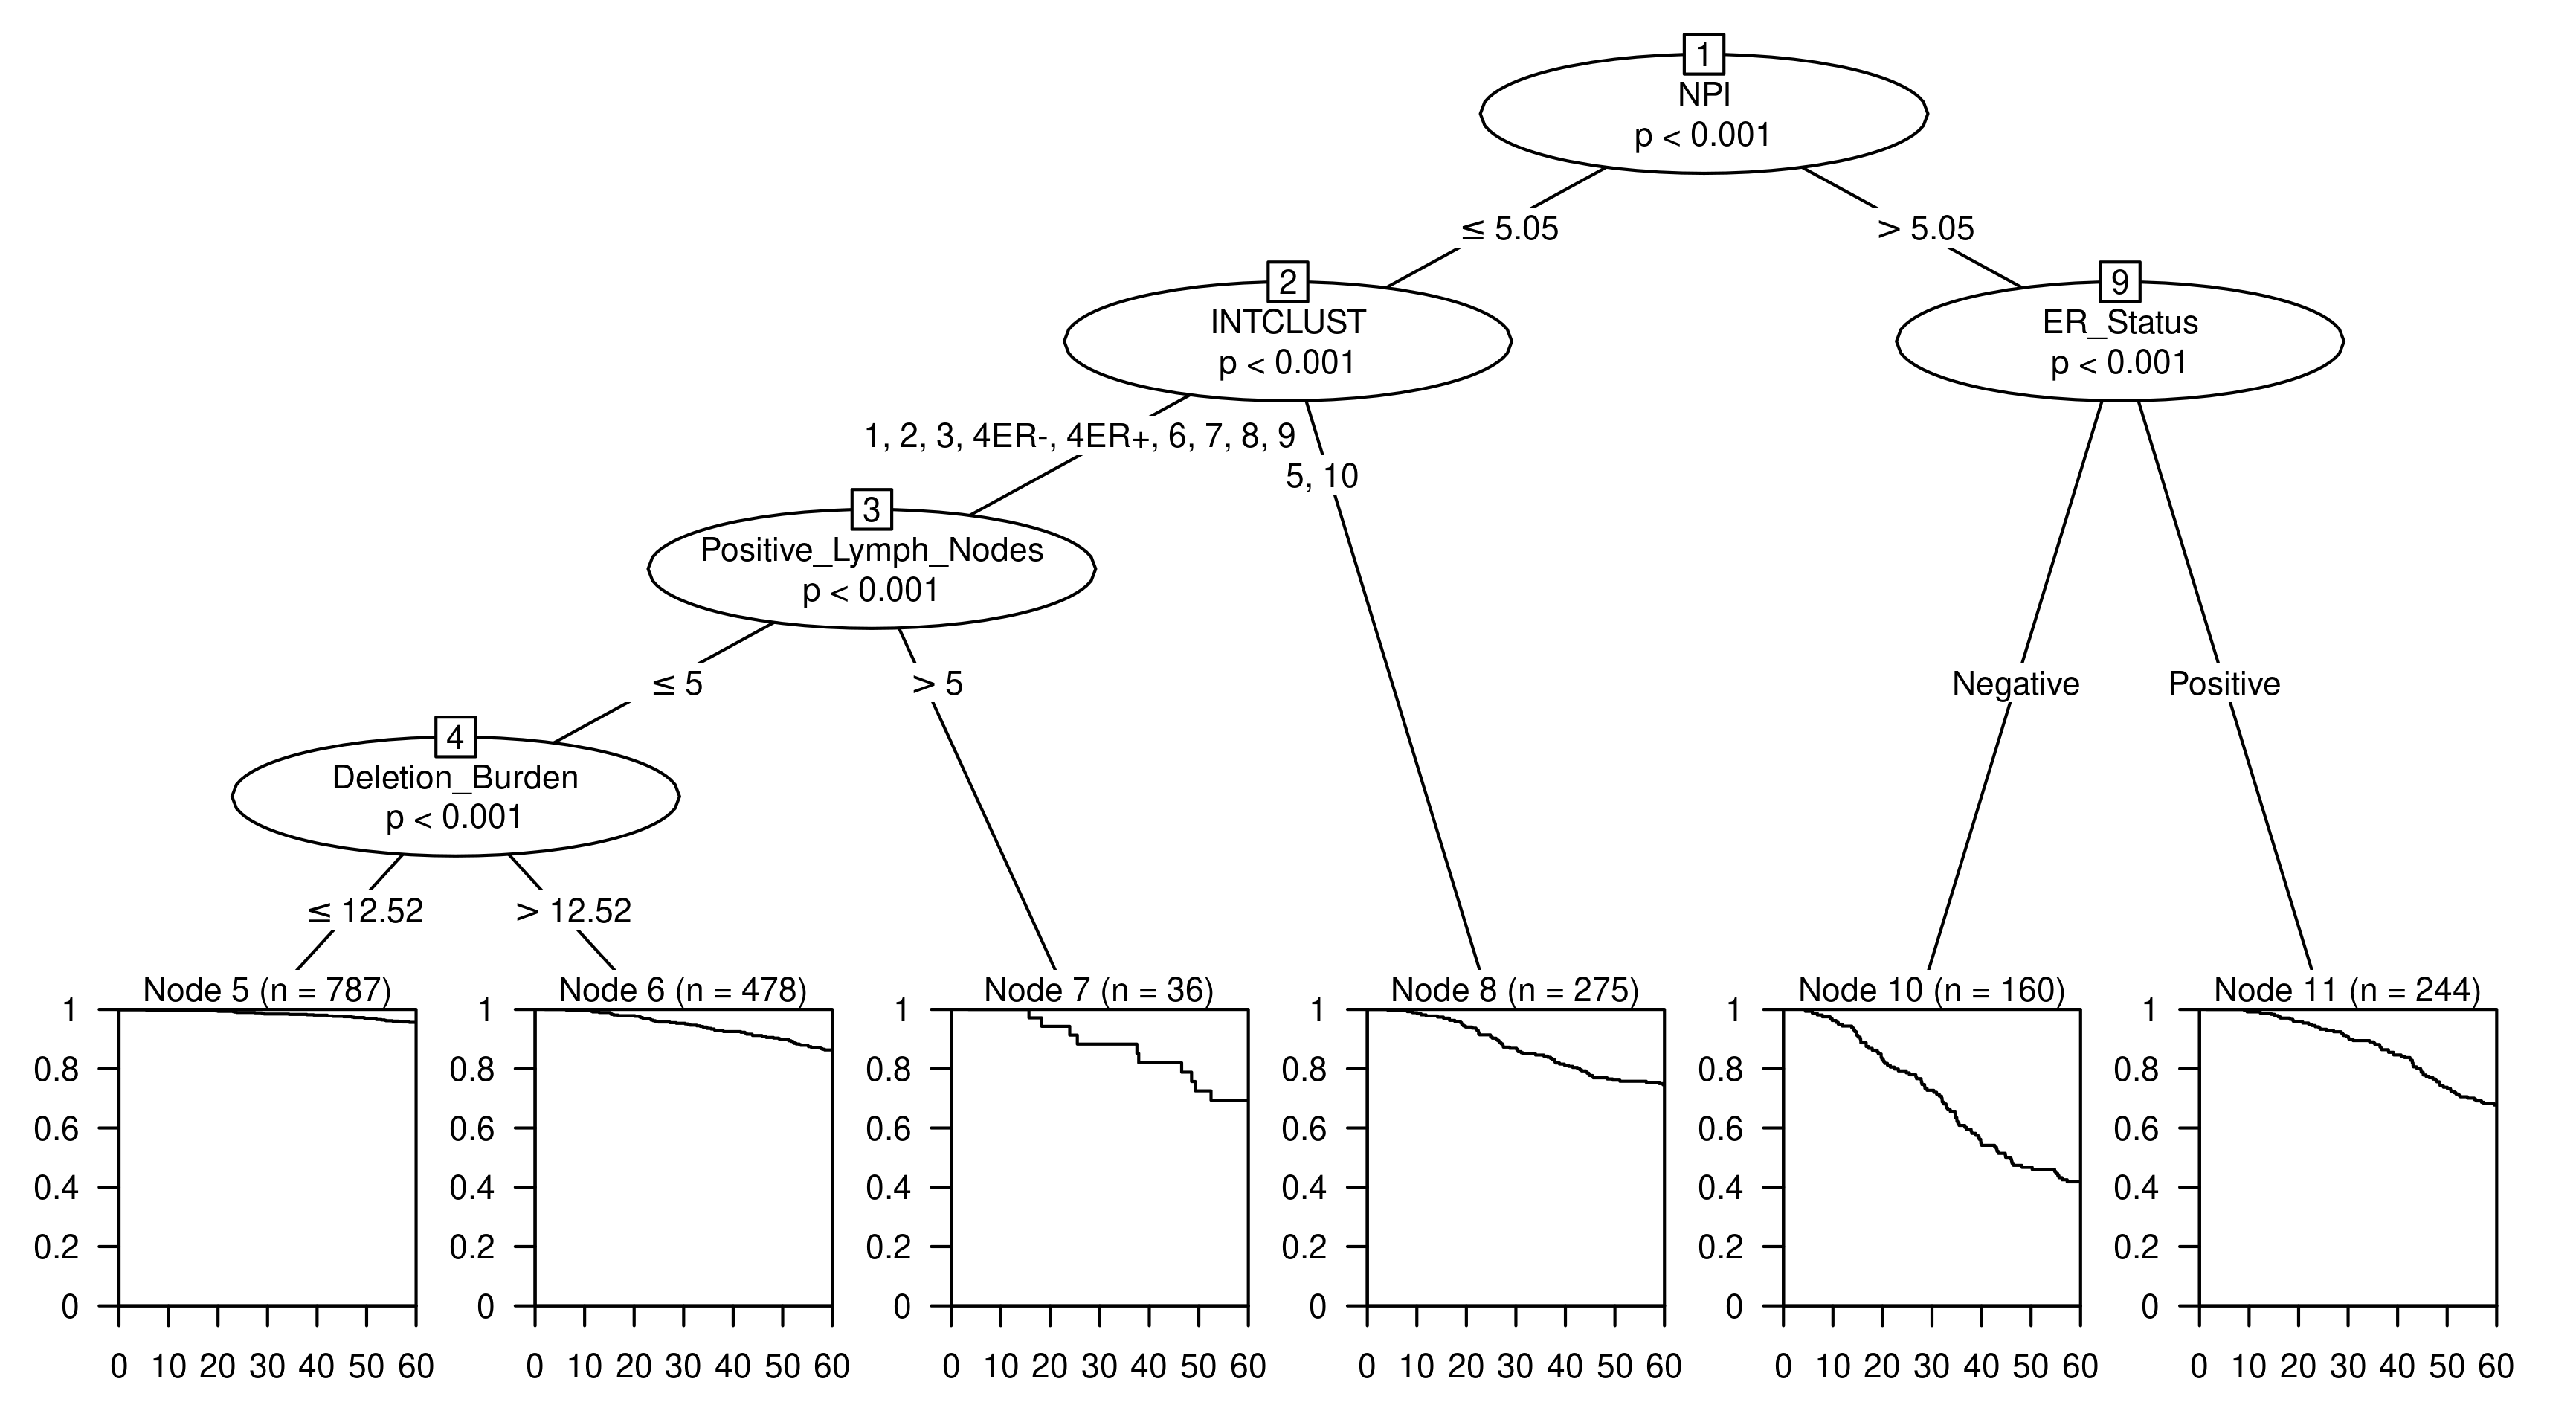
\includegraphics[width=1\textwidth]{../figures/Chapter_3/Clin_Ctree_Survival_Burden_FiveYearDSS_INTCLUST.png}
\end{subfigure}

\vspace{1cm}

\caption[Recursive partitioning survival trees for five-year disease-specific survival using Integrative Cluster, the six CNA Burden metrics and a number of clinical variables as candidate predictors.]{Recursive partitioning survival trees for five-year disease-specific survival using Integrative Cluster, the six CNA Burden metrics and a number of clinical variables as candidate predictors. (A) Trees fitted using the rpart algorithm and (B) trees fitted using the ctree algorithm.}
\label{fig:INTCLUST_CNA_Burden_FiveYearDSS_Clin}
\end{figure}

\begin{figure}[!h]
\centering

\vspace{1cm}

\begin{subfigure}{\textwidth}
\subcaption{}
\includegraphics[width=1\textwidth]{../figures/Chapter_3/Clin_PartyKit_Survival_Burden_TenYearDSS_INTCLUST.png}
\end{subfigure}

\vspace{3cm}

\begin{subfigure}{\textwidth}
\subcaption{}
\includegraphics[width=1\textwidth]{../figures/Chapter_3/Clin_Ctree_Survival_Burden_TenYearDSS_INTCLUST.png}
\end{subfigure}

\vspace{1cm}

\caption[Recursive partitioning survival trees for ten-year disease-specific survival using Integrative Cluster, the six CNA Burden metrics and a number of clinical variables as candidate predictors.]{Recursive partitioning survival trees for ten-year disease-specific survival using Integrative Cluster, the six CNA Burden metrics and a number of clinical variables as candidate predictors. (A) Trees fitted using the rpart algorithm and (B) trees fitted using the ctree algorithm.}
\label{fig:INTCLUST_CNA_Burden_TenYearDSS_Clin}
\end{figure}

\subsubsection{CNA Metric Survival Trees, in Combination with Molecular Classification and Clinical Predictors}
To assess how the addition of clinical variables alters the observed partitioning and explore interactions between the clinical variables and CNA metrics in modelling DSS, 5-year DSS and 10-year DSS, survival trees including the six CNA Burden metrics, IntClust or PAM50 molecular classification, and selected clinical variables as candidate predictors are fitted (Figures \ref{fig:PAM50_CNA_Burden_DSS_Clin}-\ref{fig:INTCLUST_CNA_Burden_TenYearDSS_Clin}). To avoid overcrowding, these trees are limited to a depth of four, where depth is defined as the number of layers or levels in the tree. While the CNA Score and CNA Burden trees partition the data similarly, it is observed that there is more consensus among the CNA Burden trees produced across different survival times and using different algorithms. Based on this and the fact that CNA Burden is a standardised metric, i.e. all patients have CNA Burden in the range 0 to 100, we show only the survival trees including CNA Burden, IntClust or PAM50 molecular classification, and selected clinical variables, as candidate predictors. The clinical variables selected are number of positive lymph nodes, NPI, ER Status, PR Status, HER2 Status, age, tumour size, tumour stage, tumour grade and cancer type.  

Figures \ref{fig:PAM50_CNA_Burden_DSS_Clin}-\ref{fig:PAM50_CNA_Burden_TenYearDSS_Clin} display survival trees for DSS, 5-year DSS and 10-year DSS, that have the six CNA Burden metrics, PAM50 molecular classification and the selected clinical variables as candidate predictors. It is observed that total CNA Burden, CNA Del Burden and Percentage Amp Burden, appear as significant predictors in the context of the DSS, in addition to PAM50 subtype and a number of clinical variables including NPI, number of positive lymph nodes, age and ER status.

For DSS, CNA Burden provides additional information for patients who have NPI $< 5.05$, and for patients who have NPI $< 5.05$ and $\leq 1$ positive lymph node, for the rpart and ctree algorithms, respectively (Figure \ref{fig:PAM50_CNA_Burden_DSS_Clin}). The CNA Burden threshold for both partitions are 24.91\% and 24.90\%. For the 5-year DSS survival trees, fitted with the rpart algorithm, CNA Burden with threshold 24.56\% is used \FloatBarrier \noindent to partition the patients with NPI $< 4.05$ and CNA Del Burden is used to partition patients with NPI $\geq 4.05$ and ER positivity, with threshold 10.85\% (Figure \ref{fig:PAM50_CNA_Burden_FiveYearDSS_Clin}A). For the 5-year DSS survival trees, fitted with the ctree algorithm, CNA Del Burden, with threshold 16.52\%, is used to split patients with NPI $\leq 5.05$ who correspond to the Claudin-low, Luminal A, Luminal B and Normal PAM50 subtypes (Figure \ref{fig:PAM50_CNA_Burden_FiveYearDSS_Clin}B). Similar partitions are observed in the 10-year DSS trees (Figure \ref{fig:PAM50_CNA_Burden_TenYearDSS_Clin}), where CNA Burden and CNA Del Burden are utilised in sub-partitions of the trees. Interestingly, even with the addition of traditionally used clinical variables, the CNA Burden metrics still appear useful in stratifying patients based on DSS, 5-year and 10-year DSS. In particular, CNA Del Burden is again used to partition Luminal A, Claudin-low and Normal patients. In all cases, patients in the partition corresponding to the lower GI have better disease-specific survival outcomes.

Focusing on survival trees for DSS, 5-year DSS and 10-year DSS, that have the six CNA Burden metrics, IntClust molecular classification and the selected clinical variables as candidate predictors, similar tree structures are observed. Again, CNA Burden, CNA Del Burden and Percentage Amp Burden appear to be useful in stratifying patients in the context of disease-specific survival (Figures \ref{fig:INTCLUST_CNA_Burden_DSS_Clin}-\ref{fig:INTCLUST_CNA_Burden_TenYearDSS_Clin}). 

\subsection{Analysis of Chromosome Arm CNA Metrics across All METABRIC Patients}
\label{Trees_Arm}
In addition to expanding the study focus to all patients, we also broaden the analysis by using the 42 chromosome arm CNA Score and Burden metrics as candidate predictors in the survival trees. These chromosome arm CNA metrics are initially included with PAM50 or IntClust molecular classifications to assess whether the chromosome arm CNA metric information can add additional prognostic value to the molecular classifications, and then included with a selection of clinical variables to explore interactions between the clinical variables and CNA metrics.

\subsubsection{Chromosome Arm CNA Metric Survival Trees in Combination with Molecular Classification Predictors}
There was less consistency observed in the survival trees produced using the chromosome arm CNA metrics than in the survival trees using the global CNA metrics. This may be due to the increased number of candidate predictors used in the chromosome arm CNA metric survival trees (43 candidate predictors) compared to the global CNA metric survival trees where seven predictors are included. Including the 42 chromosome arm CNA metrics, along with PAM50 or IntClust molecular classification, as candidate predictors enables us to determine if the CNA Score or Burden on specific chromosome arms is useful in stratifying patients on DSS, 5-year DSS and 10-year DSS outcomes.  

Focusing on the survival trees including the CNA Score metrics (Figure \ref{fig:PAM50_PA_CNA_Score_DSS}-\ref{fig:PAM50_PA_CNA_Score_TenYearDSS}), it is noted that all trees initially split on PAM50 subtype followed by either one or more of the CNA Score metrics, or PAM50 subtype again. While variation is observed between trees for DSS, 5-year DSS and 10-year DSS, CNA Score metrics corresponding to chromosome 3p and 18q appear most frequently as important predictors for DSS. 

For example, the CNA Difference Score and CNA Del Score landscape on chromosome 3p is useful in stratifying patients (Figures \ref{fig:PAM50_PA_CNA_Score_DSS} and \ref{fig:PAM50_PA_CNA_Score_TenYearDSS}). Luminal A and Claudin-low patients with a 3p CNA Difference Score $<-5.5$ or CNA Del Score $>184$, have reduced DSS when compared to patients with CNA Difference Score $\geq -5.5$ or CNA Del Score $\leq 184$, respectively (Figure \ref{fig:PAM50_PA_CNA_Score_DSS}). CNA Difference Score and CNA Del Score on chromosome 3p also appear as significant predictors of 10-year DSS survival, with thresholds -6.5 and 6, respectively (Figure \ref{fig:PAM50_PA_CNA_Score_TenYearDSS}). 

Chromosome 18q CNA Score metrics also appear as useful predictors of survival across PAM50 subtypes, mainly Claudin-low, Luminal A, Luminal B and Normal patients (Figures \ref{fig:PAM50_PA_CNA_Score_FiveYearDSS} and \ref{fig:PAM50_PA_CNA_Score_TenYearDSS}). Claudin-low, Luminal A, Luminal B and Normal patients with Percentage Del Score on chromosome 18q $>55.56\%$ have decreased 5-year DSS. Patients with Percentage Del Score on chromosome 18q $\leq 55.56\%$ are further partitioned based on CNA Del Score on chromosome 4p and then on PAM50 subtype (Figure \ref{fig:PAM50_PA_CNA_Score_FiveYearDSS}). In terms of 10-year DSS, CNA Del Score on chromosome 18q is useful in stratifying Claudin-low, Luminal A and Normal patients with CNA Del Score on chromosome 3p $\leq 6$ and CNA Amp Score on 11q $\leq 298$ (Figure \ref{fig:PAM50_PA_CNA_Score_TenYearDSS}). Patients in these groups, with 18q CNA Del Score $> 191$ have worse 10-year DSS survival outcomes than patients with CNA Del Score below this threshold. Other chromosome arm CNA Scores observed include CNA Del Score on chromosome 11p, partitioning Luminal A patients with a threshold of 38.5 and CNA Score on chromosome 17p, partitioning Claudin-low, Luminal B and Normal patients with a threshold of 5 (Figure \ref{fig:PAM50_PA_CNA_Score_FiveYearDSS}). 

The survival trees generated using the CNA Burden metrics and PAM50 subtype as candidate predictors partition the patients similarly to the CNA Score survival trees, with high congruence seen in the chromosome arm metrics highlighted as useful predictors of survival (Figure \ref{fig:PAM50_PA_CNA_Burden_DSS}-\ref{fig:PAM50_PA_CNA_Burden_TenYearDSS}). For example, the CNA Del Burden landscape on chromosome 3p is again identified as a useful predictor in stratifying patients (Figure \ref{fig:PAM50_PA_CNA_Burden_DSS} and \ref{fig:PAM50_PA_CNA_Burden_TenYearDSS}). Luminal A and Claudin-low patients with a 3p CNA Del burden higher than 30.21\% have reduced DSS when compared to patients with lower 3p CNA Del burden (Figure \ref{fig:PAM50_PA_CNA_Burden_DSS}B). This highlights that irrespective of using CNA Del Score on chromosome 3p with threshold 184 (Figure \ref{fig:PAM50_PA_CNA_Score_DSS}B) or CNA Del Burden with a threshold of 30.21\%  (Figure \ref{fig:PAM50_PA_CNA_Burden_DSS}B), Claudin-low and Luminal A patients are partitioned into Node 4 with n = 794 and Node 5 with n = 128.   

The majority of the chromosome CNA Score and Burden metrics selected as useful predictors corresponded to either the deletion or difference metrics. This is similar to what was observed in the survival trees including the global CNA Score and Burden metrics as candidate predictors: patients that have chromosome arm CNA Score and Burden metrics above the optimised threshold have worse survival outcomes.

Focusing on the survival trees including IntClust classification and CNA Score metrics (Figure \ref{fig:INTCLUST_PA_CNA_Score_DSS}-\ref{fig:INTCLUST_PA_CNA_Score_TenYearDSS}), it is observed that all trees initially split on IntClust classification, grouping IntClust 1, 2, 4ER-, 5, 6, 9, 10 together and IntClust 3, 4ER+, 7 and 8 together, followed by CNA Del Score on chromosome 18q, and in some cases, other chromosome arm CNA Score metrics. CNA Del Score on chromosome 18q, with a threshold of $\approx 160$, consistently appears as an important predictor for DSS, 5-year DSS and 10-year DSS. For example, CNA Del Score on chromosome 18q partitions IntClust 3, 4ER+, 7 and 8 patients into two groups, $\geq 160.5$ and $<160.5$ (Figure \ref{fig:INTCLUST_PA_CNA_Score_DSS}A and Figure \ref{fig:INTCLUST_PA_CNA_Score_TenYearDSS}A). Similar to what is observed in previously fitted survival trees, patients that have CNA Del Score above an optimised threshold have poorer survival outcomes. In trees where patients were partitioned using additional chromosome arm CNA Score metrics, CNA Score on chromosome 1p, CNA Amp Score on 6q, CNA Amp Score on 12p, CNA Del Score on 4p, CNA Score on 11q and Difference Score on 1p, appear as useful predictors. 

The survival trees including the CNA Burden metrics and IntClust molecular classification as candidate predictors, are similar to the trees including the CNA Score metrics (Figure \ref{fig:INTCLUST_PA_CNA_Burden_DSS}-\ref{fig:INTCLUST_PA_CNA_Burden_TenYearDSS}). 

The chromosome arms that were selected across the survival trees as useful predictors in the context of DSS, 5-year DSS and 10-year DSS, were chromosome arms 1p, 3p, 4p, 6q, 11p, 11q, 17p, 17q and 18q. However, CNA Del and Difference metrics on chromosome 3p, and CNA Del metrics on 18q are the predictors that appear most frequently across the chromosome arm CNA Score and Burden metric survival trees. In agreement with the global CNA Score Burden survival trees, the patients are partitioned initially on PAM50 subtypes and IntClusts, where subtypes or clusters that display low genomic instability and generally good prognosis are grouped together. Subsequently these patients are partitioned, using one or more of the CNA metrics (primarily CNA Del metrics) at an optimal cut-off point.

\begin{figure}[!h]
\centering

\vspace{0.5cm}

\begin{subfigure}{\textwidth}
\subcaption{}
\includegraphics[width=1\textwidth]{../figures/Chapter_3/PA_PartyKit_Survival_Score_DSS_PAM50.png}
\end{subfigure}

\vspace{2cm}

\begin{subfigure}{\textwidth}
\subcaption{}
\includegraphics[width=1\textwidth]{../figures/Chapter_3/PA_Ctree_Survival_Score_DSS_PAM50.png}
\end{subfigure}

\vspace{0.5cm}

\caption[Recursive partitioning survival trees for disease-specific survival using PAM50 subtype and the 42 chromosome arm CNA Score metrics as candidate predictors.]{Recursive partitioning survival trees for disease-specific survival using PAM50 subtype and the 42 chromosome arm CNA Score metrics as candidate predictors. (A) Trees fitted using the rpart algorithm and (B) trees fitted using the ctree algorithm.}
\label{fig:PAM50_PA_CNA_Score_DSS}
\end{figure}

\begin{figure}[!h]
\centering

\vspace{0.5cm}

\begin{subfigure}{\textwidth}
\subcaption{}
\includegraphics[width=1\textwidth]{../figures/Chapter_3/PA_PartyKit_Survival_Score_FiveYearDSS_PAM50.png}
\end{subfigure}

\vspace{2cm}

\begin{subfigure}{\textwidth}
\subcaption{}
\includegraphics[width=1\textwidth]{../figures/Chapter_3/PA_Ctree_Survival_Score_FiveYearDSS_PAM50.png}
\end{subfigure}

\vspace{0.5cm}

\caption[Recursive partitioning survival trees for five-year disease-specific survival using PAM50 subtype and the 42 chromosome arm CNA Score metrics as candidate predictors.]{Recursive partitioning survival trees for five-year disease-specific survival using PAM50 subtype and the 42 chromosome arm CNA Score metrics as candidate predictors. (A) Trees fitted using the rpart algorithm and (B) trees fitted using the ctree algorithm.}
\label{fig:PAM50_PA_CNA_Score_FiveYearDSS}
\end{figure}


\begin{figure}[!h]
\centering

\vspace{0.5cm}

\begin{subfigure}{\textwidth}
\subcaption{}
\includegraphics[width=1\textwidth]{../figures/Chapter_3/PA_PartyKit_Survival_Score_TenYearDSS_PAM50.png}
\end{subfigure}

\vspace{2cm}

\begin{subfigure}{\textwidth}
\subcaption{}
\includegraphics[width=1\textwidth]{../figures/Chapter_3/PA_Ctree_Survival_Score_TenYearDSS_PAM50.png}
\end{subfigure}

\vspace{0.5cm}

\caption[Recursive partitioning survival trees for five-year disease-specific survival using PAM50 subtype and the 42 chromosome arm CNA Score metrics as candidate predictors.]{Recursive partitioning survival trees for five-year disease-specific survival using PAM50 subtype and the 42 chromosome arm CNA Score metrics as candidate predictors. (A) Trees fitted using the rpart algorithm and (B) trees fitted using the ctree algorithm.}
\label{fig:PAM50_PA_CNA_Score_TenYearDSS}
\end{figure}

\begin{figure}[!h]
\centering

\vspace{0.5cm}

\begin{subfigure}{\textwidth}
\subcaption{}
\includegraphics[width=1\textwidth]{../figures/Chapter_3/PA_PartyKit_Survival_Burden_DSS_PAM50.png}
\end{subfigure}

\vspace{2cm}

\begin{subfigure}{\textwidth}
\subcaption{}
\includegraphics[width=1\textwidth]{../figures/Chapter_3/PA_Ctree_Survival_Burden_DSS_PAM50.png}
\end{subfigure}

\vspace{0.5cm}

\caption[Recursive partitioning survival trees for disease-specific survival using PAM50 subtype and the 42 chromosome arm CNA Burden metrics as candidate predictors.]{Recursive partitioning survival trees for disease-specific survival using PAM50 subtype and the 42 chromosome arm CNA Burden metrics as candidate predictors. (A) Trees fitted using the rpart algorithm and (B) trees fitted using the ctree algorithm.}
\label{fig:PAM50_PA_CNA_Burden_DSS}
\end{figure}

\begin{figure}[!h]
\centering

\vspace{0.5cm}

\begin{subfigure}{\textwidth}
\subcaption{}
\includegraphics[width=1\textwidth]{../figures/Chapter_3/PA_PartyKit_Survival_Burden_FiveYearDSS_PAM50.png}
\end{subfigure}

\vspace{2cm}

\begin{subfigure}{\textwidth}
\subcaption{}
\includegraphics[width=1\textwidth]{../figures/Chapter_3/PA_Ctree_Survival_Burden_FiveYearDSS_PAM50.png}
\end{subfigure}

\vspace{0.5cm}

\caption[Recursive partitioning survival trees for five-year disease-specific survival using PAM50 subtype and the 42 chromosome arm CNA Burden metrics as candidate predictors.]{Recursive partitioning survival trees for five-year disease-specific survival using PAM50 subtype and the 42 chromosome arm CNA Burden metrics as candidate predictors. (A) Trees fitted using the rpart algorithm and (B) trees fitted using the ctree algorithm.}
\label{fig:PAM50_PA_CNA_Burden_FiveYearDSS}
\end{figure}

\begin{figure}[!h]
\centering

\vspace{0.5cm}

\begin{subfigure}{\textwidth}
\subcaption{}
\includegraphics[width=1\textwidth]{../figures/Chapter_3/PA_PartyKit_Survival_Burden_TenYearDSS_PAM50.png}
\end{subfigure}

\vspace{2cm}

\begin{subfigure}{\textwidth}
\subcaption{}
\includegraphics[width=1\textwidth]{../figures/Chapter_3/PA_Ctree_Survival_Burden_TenYearDSS_PAM50.png}
\end{subfigure}

\vspace{0.5cm}

\caption[Recursive partitioning survival trees for five-year disease-specific survival using PAM50 subtype and the 42 chromosome arm CNA Burden metrics as candidate predictors.]{Recursive partitioning survival trees for five-year disease-specific survival using PAM50 subtype and the 42 chromosome arm CNA Burden metrics as candidate predictors. (A) Trees fitted using the rpart algorithm and (B) trees fitted using the ctree algorithm.}
\label{fig:PAM50_PA_CNA_Burden_TenYearDSS}
\end{figure}

\begin{figure}[!h]
\centering

\vspace{0.5cm}

\begin{subfigure}{\textwidth}
\subcaption{}
\includegraphics[width=1\textwidth]{../figures/Chapter_3/PA_PartyKit_Survival_Score_DSS_INTCLUST.png}
\end{subfigure}

\vspace{2cm}

\begin{subfigure}{\textwidth}
\subcaption{}
\includegraphics[width=1\textwidth]{../figures/Chapter_3/PA_Ctree_Survival_Score_DSS_INTCLUST.png}
\end{subfigure}

\vspace{0.5cm}

\caption[Recursive partitioning survival trees for disease-specific survival using Integrative Cluster and the 42 chromosome arm CNA Score metrics as candidate predictors.]{Recursive partitioning survival trees for disease-specific survival using Integrative Cluster and the 42 chromosome arm CNA Score metrics as candidate predictors. (A) Trees fitted using the rpart algorithm and (B) trees fitted using the ctree algorithm.}
\label{fig:INTCLUST_PA_CNA_Score_DSS}
\end{figure}

\begin{figure}[!h]
\centering

\vspace{0.5cm}

\begin{subfigure}{\textwidth}
\subcaption{}
\includegraphics[width=1\textwidth]{../figures/Chapter_3/PA_PartyKit_Survival_Score_FiveYearDSS_INTCLUST.png}
\end{subfigure}

\vspace{2cm}

\begin{subfigure}{\textwidth}
\subcaption{}
\includegraphics[width=1\textwidth]{../figures/Chapter_3/PA_Ctree_Survival_Score_FiveYearDSS_INTCLUST.png}
\end{subfigure}

\vspace{0.5cm}

\caption[Recursive partitioning survival trees for five-year disease-specific survival using Integrative Cluster and the 42 chromosome arm CNA Score metrics as candidate predictors.]{Recursive partitioning survival trees for five-year disease-specific survival using Integrative Cluster and the 42 chromosome arm CNA Score metrics as candidate predictors. (A) Trees fitted using the rpart algorithm and (B) trees fitted using the ctree algorithm.}
\label{fig:INTCLUST_PA_CNA_Score_FiveYearDSS}
\end{figure}


\begin{figure}[!h]
\centering

\vspace{0.5cm}

\begin{subfigure}{\textwidth}
\subcaption{}
\includegraphics[width=1\textwidth]{../figures/Chapter_3/PA_PartyKit_Survival_Score_TenYearDSS_INTCLUST.png}
\end{subfigure}

\vspace{2cm}

\begin{subfigure}{\textwidth}
\subcaption{}
\includegraphics[width=1\textwidth]{../figures/Chapter_3/PA_Ctree_Survival_Score_TenYearDSS_INTCLUST.png}
\end{subfigure}

\vspace{0.5cm}

\caption[Recursive partitioning survival trees for five-year disease-specific survival using Integrative Cluster and the 42 chromosome arm CNA Score metrics as candidate predictors.]{Recursive partitioning survival trees for five-year disease-specific survival using  Integrative Cluster and the 42 chromosome arm CNA Score metrics as candidate predictors. (A) Trees fitted using the rpart algorithm and (B) trees fitted using the ctree algorithm.}
\label{fig:INTCLUST_PA_CNA_Score_TenYearDSS}
\end{figure}


\begin{figure}[!h]
\centering

\vspace{0.5cm}

\begin{subfigure}{\textwidth}
\subcaption{}
\includegraphics[width=1\textwidth]{../figures/Chapter_3/PA_PartyKit_Survival_Burden_DSS_INTCLUST.png}
\end{subfigure}

\vspace{2cm}

\begin{subfigure}{\textwidth}
\subcaption{}
\includegraphics[width=1\textwidth]{../figures/Chapter_3/PA_Ctree_Survival_Burden_DSS_INTCLUST.png}
\end{subfigure}

\vspace{0.5cm}

\caption[Recursive partitioning survival trees for disease-specific survival using Integrative Cluster and the 42 chromosome arm CNA Burden metrics as candidate predictors.]{Recursive partitioning survival trees for disease-specific survival using Integrative Cluster and the 42 chromosome arm CNA Burden metrics as candidate predictors. (A) Trees fitted using the rpart algorithm and (B) trees fitted using the ctree algorithm.}
\label{fig:INTCLUST_PA_CNA_Burden_DSS}
\end{figure}

\begin{figure}[!h]
\centering

\vspace{0.5cm}

\begin{subfigure}{\textwidth}
\subcaption{}
\includegraphics[width=1\textwidth]{../figures/Chapter_3/PA_PartyKit_Survival_Burden_FiveYearDSS_INTCLUST.png}
\end{subfigure}

\vspace{2cm}

\begin{subfigure}{\textwidth}
\subcaption{}
\includegraphics[width=1\textwidth]{../figures/Chapter_3/PA_Ctree_Survival_Burden_FiveYearDSS_INTCLUST.png}
\end{subfigure}

\vspace{0.5cm}

\caption[Recursive partitioning survival trees for five-year disease-specific survival using Integrative Cluster and the 42 chromosome arm CNA Burden metrics as candidate predictors.]{Recursive partitioning survival trees for five-year disease-specific survival using Integrative Cluster and the 42 chromosome arm CNA Burden metrics as candidate predictors. (A) Trees fitted using the rpart algorithm and (B) trees fitted using the ctree algorithm.}
\label{fig:INTCLUST_PA_CNA_Burden_FiveYearDSS}
\end{figure}


\begin{figure}[!h]
\centering

\vspace{0.5cm}

\begin{subfigure}{\textwidth}
\subcaption{}
\includegraphics[width=1\textwidth]{../figures/Chapter_3/PA_PartyKit_Survival_Burden_TenYearDSS_INTCLUST.png}
\end{subfigure}

\vspace{2cm}

\begin{subfigure}{\textwidth}
\subcaption{}
\includegraphics[width=1\textwidth]{../figures/Chapter_3/PA_Ctree_Survival_Burden_TenYearDSS_INTCLUST.png}
\end{subfigure}

\vspace{0.5cm}

\caption[Recursive partitioning survival trees for five-year disease-specific survival using Integrative Cluster and the 42 chromosome arm CNA Burden metrics as candidate predictors.]{Recursive partitioning survival trees for five-year disease-specific survival using  Integrative Cluster and the 42 chromosome arm CNA Burden metrics as candidate predictors. (A) Trees fitted using the rpart algorithm and (B) trees fitted using the ctree algorithm.}
\label{fig:INTCLUST_PA_CNA_Burden_TenYearDSS}
\end{figure}

\begin{figure}[!h]
\centering

\vspace{1cm}

\begin{subfigure}{\textwidth}
\subcaption{}
\includegraphics[width=1\textwidth]{../figures/Chapter_3/Clin_PA_PartyKit_Survival_Burden_DSS_PAM50.png}
\end{subfigure}

\vspace{2cm}

\begin{subfigure}{\textwidth}
\subcaption{}
\includegraphics[width=1\textwidth]{../figures/Chapter_3/Clin_PA_Ctree_Survival_Burden_DSS_PAM50.png}
\end{subfigure}

\vspace{1cm}

\caption[Recursive partitioning survival trees for disease-specific survival using PAM50 subtype, the 42 CNA Burden metrics and a number of clinical variables as candidate predictors.]{Recursive partitioning survival trees for disease-specific survival using PAM50 subtype, the 42 CNA Burden metrics and a number of clinical variables as candidate predictors. (A) Trees fitted using the rpart algorithm and (B) trees fitted using the ctree algorithm.}
\label{fig:PA_PAM50_CNA_Burden_DSS_Clin}
\end{figure}

\begin{figure}[!h]
\centering

\vspace{1cm}

\begin{subfigure}{\textwidth}
\subcaption{}
\includegraphics[width=1\textwidth]{../figures/Chapter_3/Clin_PA_PartyKit_Survival_Burden_FiveYearDSS_PAM50.png}
\end{subfigure}

\vspace{2cm}

\begin{subfigure}{\textwidth}
\subcaption{}
\includegraphics[width=1\textwidth]{../figures/Chapter_3/Clin_PA_Ctree_Survival_Burden_FiveYearDSS_PAM50.png}
\end{subfigure}

\vspace{1cm}

\caption[Recursive partitioning survival trees for five-year disease-specific survival using PAM50 subtype, the 42 CNA Burden metrics and a number of clinical variables as candidate predictors.]{Recursive partitioning survival trees for five-year disease-specific survival using PAM50 subtype, the 42 CNA Burden metrics and a number of clinical variables as candidate predictors. (A) Trees fitted using the rpart algorithm and (B) trees fitted using the ctree algorithm.}
\label{fig:PA_PAM50_CNA_Burden_FiveYearDSS_Clin}
\end{figure}

\begin{figure}[!h]
\centering

\vspace{1cm}

\begin{subfigure}{\textwidth}
\subcaption{}
\includegraphics[width=1\textwidth]{../figures/Chapter_3/Clin_PA_PartyKit_Survival_Burden_TenYearDSS_PAM50.png}
\end{subfigure}

\vspace{2cm}

\begin{subfigure}{\textwidth}
\subcaption{}
\includegraphics[width=1\textwidth]{../figures/Chapter_3/Clin_PA_Ctree_Survival_Burden_TenYearDSS_PAM50.png}
\end{subfigure}

\vspace{1cm}

\caption[Recursive partitioning survival trees for ten-year disease-specific survival using PAM50 subtype, the 42 CNA Burden metrics and a number of clinical variables as candidate predictors.]{Recursive partitioning survival trees for ten-year disease-specific survival using PAM50 subtype, the 42 CNA Burden metrics and a number of clinical variables as candidate predictors. (A) Trees fitted using the rpart algorithm and (B) trees fitted using the ctree algorithm.}
\label{fig:PA_PAM50_CNA_Burden_TenYearDSS_Clin}
\end{figure}


\begin{figure}[!h]
\centering

\vspace{1cm}

\begin{subfigure}{\textwidth}
\subcaption{}
\includegraphics[width=1\textwidth]{../figures/Chapter_3/Clin_PA_PartyKit_Survival_Burden_DSS_INTCLUST.png}
\end{subfigure}

\vspace{2cm}

\begin{subfigure}{\textwidth}
\subcaption{}
\includegraphics[width=1\textwidth]{../figures/Chapter_3/Clin_PA_Ctree_Survival_Burden_DSS_INTCLUST.png}
\end{subfigure}

\vspace{1cm}

\caption[Recursive partitioning survival trees for disease-specific survival using Integrative Cluster, the 42 CNA Burden metrics and a number of clinical variables as candidate predictors.]{Recursive partitioning survival trees for disease-specific survival using Integrative Cluster, the 42 CNA Burden metrics and a number of clinical variables as candidate predictors. (A) Trees fitted using the rpart algorithm and (B) trees fitted using the ctree algorithm.}
\label{fig:PA_INTCLUST_CNA_Burden_DSS_Clin}
\end{figure}

\begin{figure}[!h]
\centering

\vspace{1cm}

\begin{subfigure}{\textwidth}
\subcaption{}
\includegraphics[width=1\textwidth]{../figures/Chapter_3/Clin_PA_PartyKit_Survival_Burden_FiveYearDSS_INTCLUST.png}
\end{subfigure}

\vspace{2cm}

\begin{subfigure}{\textwidth}
\subcaption{}
\includegraphics[width=1\textwidth]{../figures/Chapter_3/Clin_PA_Ctree_Survival_Burden_FiveYearDSS_INTCLUST.png}
\end{subfigure}

\vspace{1cm}

\caption[Recursive partitioning survival trees for five-year disease-specific survival using Integrative Cluster, the 42 CNA Burden metrics and a number of clinical variables as candidate predictors.]{Recursive partitioning survival trees for five-year disease-specific survival using Integrative Cluster, the 42 CNA Burden metrics and a number of clinical variables as candidate predictors. (A) Trees fitted using the rpart algorithm and (B) trees fitted using the ctree algorithm.}
\label{fig:PA_INTCLUST_CNA_Burden_FiveYearDSS_Clin}
\end{figure}

\begin{figure}[!h]
\centering

\vspace{1cm}

\begin{subfigure}{\textwidth}
\subcaption{}
\includegraphics[width=1\textwidth]{../figures/Chapter_3/Clin_PA_PartyKit_Survival_Burden_TenYearDSS_INTCLUST.png}
\end{subfigure}

\vspace{2cm}

\begin{subfigure}{\textwidth}
\subcaption{}
\includegraphics[width=1\textwidth]{../figures/Chapter_3/Clin_PA_Ctree_Survival_Burden_TenYearDSS_INTCLUST.png}
\end{subfigure}

\vspace{1cm}

\caption[Recursive partitioning survival trees for ten-year disease-specific survival using Integrative Cluster, the 42 CNA Burden metrics and a number of clinical variables as candidate predictors.]{Recursive partitioning survival trees for ten-year disease-specific survival using Integrative Cluster, the 42 CNA Burden metrics and a number of clinical variables as candidate predictors. (A) Trees fitted using the rpart algorithm and (B) trees fitted using the ctree algorithm.}
\label{fig:PA_INTCLUST_CNA_Burden_TenYearDSS_Clin}
\end{figure}

\subsubsection{Chromosome Arm CNA Metric Survival Trees in Combination with Molecular Classification and Clinical Predictors} 
To assess how the addition of clinical variables alters the observed partitioning and explore interactions between the clinical variables and CNA metrics in modelling DSS, 5-year DSS and 10-year DSS, survival trees including the six CNA Burden metrics, IntClust or PAM50 molecular classification, and selected clinical variables, are fitted (Figures \ref{fig:PA_PAM50_CNA_Burden_DSS_Clin}-\ref{fig:PA_INTCLUST_CNA_Burden_TenYearDSS_Clin}). 

The survival trees utilising the 42 chromosome arm CNA Burden metrics, PAM50 subtype, and selected clinical variables as candidate predictors indicate that a number of chromosome arm CNA Burden metrics, PAM50 subtype and several of the selected clinical variables are identified as useful predictors of DSS, 5-year DSS and 10-year DSS. All trees initially partition on NPI, with thresholds ranging from 4.05 to 5.05, and then on one or more clinical predictors, PAM50 subtype, or chromosome arm CNA Burden metric. For example, the ctree survival tree modelling DSS (Figure \ref{fig:PA_PAM50_CNA_Burden_DSS_Clin}B), partitions patients into six groups, also referred to as nodes, with Node 5 displaying the best DSS. Node 5 corresponds to patients with NPI $\leq 5.05$, number of positive lymph nodes $\leq 1$, CNA Burden on chromosome 1p $\leq 15.81$ and CNA Burden on chromosome 4p $\leq 34.09$. Despite the addition of the clinical variables, CNA Del Burden metrics on chromosome 3p and chromosome 18q are still observed in survival trees modelling 5-year DSS and 10-year DSS, particularly in Claudin-low, Luminal A, Luminal B and Normal patients (Figures \ref{fig:PA_PAM50_CNA_Burden_FiveYearDSS_Clin} and \ref{fig:PA_PAM50_CNA_Burden_TenYearDSS_Clin}). In addition, CNA Amp Burden on chromosome 9q, CNA Difference on chromosome 5q, CNA Difference on chromosome 17p, CNA Burden on 11q, CNA Burden on 16p and CNA Amp Burden on 16p also appear as useful predictors in subgroups of patients. The survival trees including the 42 chromosome arm CNA Burden metrics, IntClust molecular classification, and the selected clinical variables also consistently partition on NPI, with thresholds ranging from 4.05 to 5.05 (Figures \ref{fig:PA_INTCLUST_CNA_Burden_DSS_Clin}-\ref{fig:PA_INTCLUST_CNA_Burden_TenYearDSS_Clin}). 

Variation is observed when comparing the chromosome arm CNA Burden metrics and clinical variables selected by the recursive partitioning survival trees considering \FloatBarrier \noindent IntClust, rather than PAM50 subtype. The clinical variables used to partition the patients include combinations of NPI, number of positive lymph nodes, age, clinical stage and ER Status, while the chromosome arm metrics used to partition the data include CNA Burden on 18q, CNA Amp Burden on 9q, CNA Difference Burden on 5q, CNA Del Burden on 18q, CNA Difference on 17p, CNA Amp Burden on 6q, CNA Burden on 16p, CNA Amp Burden on chromosome 4q and CNA Amp Burden on 16p. Noticeably CNA Del Burden on chromosome 3p is absent from the survival trees considering IntClust molecular classification and initially partitioning on NPI alters the IntClust partition from consistently grouping IntClust 3, 4ER+, 7 and 8 together to a range of partitions.

Interestingly, the chromosome arm CNA Burden metrics appear as useful predictors in partitions of PAM50 subtypes and IntClusts, but also in trees and partitions where these molecular classifications were not identified as significant predictors. This indicates that the CNA Burden metrics can provide additional survival information in groups of patients split on molecular classifications and groups of patients who are not. 

\subsubsection{Heatmaps of CNA State across Selected Chromosome Arms} 
\label{Heatmaps_Chap3}
Heatmaps of the CNA landscape of chromosome 3p, chromosome 18q and chromosome 11q, with patients partitioned into nodes corresponding to Figures \ref{fig:PAM50_PA_CNA_Burden_DSS}B (ctree), \ref{fig:INTCLUST_PA_CNA_Burden_DSS}A (rpart) and \ref{fig:PAM50_PA_CNA_Burden_FiveYearDSS}A (rpart), respectively, are produced. These heatmaps provide detail of the CNA state for each of the 609, 230 and 492 genes recorded on chromosomes 3p, 18q and 11p. 

Figure \ref{PA_SurvTrees_Burden_Heatmaps_3p}, the heatmap of CNAs across chromosome 3p, shows that the Claudin-low and Luminal A patients corresponding to Node 5 have high levels of deletions across the majority of chromosome 3p, Node 4, also containing Claudin-low and Luminal A patients, consists of a small proportion of patients with high levels of amplification with the remainder being relatively stable. Node 2, containing Luminal B, HER2, Normal and Basal patients, consists of patients displaying variation in levels of GI across chromosome 3p. Figure \ref{PA_SurvTrees_Burden_Heatmaps_18q}, the heatmap of CNA calls across chromosome 18q, displays a similar pattern, where IntClust 3, 4ER+, 7 and 8 patients corresponding to Node 4 have high levels of deletions across the majority of chromosome 18q. Node 3 consists of a small proportion of IntClust 3, 4ER+, 7 and 8 patients with high levels of amplification with the remainder being relatively stable. Node 5 consists of IntClust 1, 2, 4ER-, 5, 6, 9 and 10 patients displaying variation in levels of GI across chromosome 18q. Figure \ref{PA_SurvTrees_Burden_Heatmaps_11p} displays the heatmap of CNAs across chromosome 11p. Focusing on the nodes corresponding to Luminal A patients, Nodes 3 and 4, it is observed that patients in Node 4, with worse survival outcomes, have high levels of deletions across the majority of chromosome 11p.

There are two important aspects of the data used to produce these heatmaps, including that the CNAs are only recorded for annotated genes and that the data used are total CNA data meaning it is not possible to determine whether the hemizygous CNAs observed across the chromosome arms are occurring contiguously on one homologous chromosome or if the CNAs are occurring randomly across the two. This aspect is discussed further in the upcoming chapters. 

\vfill 

\begin{figure}[H]
\vspace{0.7cm}
  \centering
  \includegraphics[width=1\textwidth]{../figures/Chapter_3/PA_Ctree_Survival_Burden_DSS_PAM50.png_3p_All_Heatmap.png}
  \caption[Heatmap of CNAs across Chromosome 3p]{Heatmap of CNAs across Chromosome 3p. The heatmap depicts the CNA state for each gene across Chromosome 3p, partitioning the patients into the nodes corresponding to Figure \ref{fig:PAM50_PA_CNA_Burden_DSS}B.}
  \label{PA_SurvTrees_Burden_Heatmaps_3p}
\end{figure}
\vspace{1cm}
\begin{figure}[H]
  \centering
  \includegraphics[width=1\textwidth]{../figures/Chapter_3/PA_PartyKit_Survival_Burden_DSS_INTCLUST.png_18q_All_Heatmap.png}
  \caption[Heatmap of CNAs across Chromosome 18q]{Heatmap of CNAs across Chromosome 18q. The heatmap depicts the CNA state for each gene across Chromosome 18q, partitioning the patients into the nodes corresponding to Figure \ref{fig:INTCLUST_PA_CNA_Burden_DSS}A.}
  \label{PA_SurvTrees_Burden_Heatmaps_18q}
\end{figure} 

\vfill 

\begin{figure}[H]
  \centering
  \includegraphics[width=1\textwidth]{../figures/Chapter_3/PA_PartyKit_Survival_Burden_FiveYearDSS_PAM50.png_11p_All_Heatmap.png}
  \caption[Heatmap of CNAs across Chromosome 11p]{Heatmap of CNAs across Chromosome 11p. The heatmap depicts the CNA state for each gene across Chromosome 11p, partitioning the patients into the nodes corresponding to Figure \ref{fig:PAM50_PA_CNA_Burden_FiveYearDSS}A.}
  \label{PA_SurvTrees_Burden_Heatmaps_11p}
\end{figure}

\subsection{GNOSIS: an R Shiny App Supporting Cancer Genomics Survival Analysis with cBioPortal}
As shown above, and in previous chapters, exploratory, statistical and survival analysis of cancer genomic data is extremely important and can lead to new discoveries, such as the identification of novel genomic prognostic markers, that have the potential to advance our understanding of cancer and ultimately benefit patients. These analyses are often performed on data available from a number of consortia websites, such cBioPortal \citep{pmid22588877, pmid23550210}, which is one of the best known and commonly used consolidated curations that hosts data from large consortium efforts. While cBioPortal provides both graphical user interface (GUI)-based and representational state transfer mediated means for researchers to explore and analyse clinical and genomics data, its capabilities have their limitations and oftentimes, to explore specific hypotheses, users need to perform a more sophisticated ‘off site’ analysis that typically requires users to have some prior programming experience. 

To overcome these limitations and provide a GUI that facilitates the visualisation and interrogation of cancer genomics data, particularly cBioPortal-hosted data, using standard biostatistical methodologies, we developed an R Shiny app called GeNomics explOrer using StatistIcal and Survival analysis in R (GNOSIS). GNOSIS was initially developed as part of our study, using the METABRIC data, to investigate whether survival outcomes are associated with genomic instability in Luminal breast cancers \citep{King_2021} and was further developed to enable the exploration, analysis and incorporation of a diverse range of genomic features with clinical data in a research or clinical setting. 

GNOSIS leverages a number of R packages and provides an intuitive GUI with multiple tab panels supporting a range of functionalities, including data upload and initial exploration, data recoding and subsetting, data visualisations, statistical analysis, mutation analysis and, in particular, survival analysis to identify prognostic markers. In addition, GNOSIS also helps researchers carry out reproducible research by providing downloadable input logs (Shiny\_Log.txt) and R scripts (ggcode.zip) from each session.  

\subsubsection{Layout and Functionality} 
The current version of GNOSIS has 11 tabs and allows users to carry out a comprehensive visual exploration, statistically robust survival analysis and mutation analysis in a simple, efficient and reproducible way. GNOSIS installs and loads up a number of R packages, primarily shiny, tidyverse, ggplot2, survival, survminer, rpart, partykit and maftools \citep{hothorn_hornik_zeileis_2006, ctree1, ggplot2,  maftools, tidyverse, survminer, rpart, shiny, survival} (see full list in Section \ref{OP}), and provides users with tabs for data upload, exploration, data subsetting and recoding, visualisations, comprehensive survival analysis, association testing and mutation analysis. In addition, GNOSIS records all user activity and provides downloadable .txt files and R scripts to facilitate reproducibility. Figure \ref{GNOSIS_Tab1} shows the GNOSIS front-end with the specific entry points and ‘tabs’ marked in red.  

\begin{figure}[!h]
\center
\includegraphics[width=1\textwidth]{../figures/Chapter_3/GNOSIS_Pic.png}
\caption[GNOSIS GUI with highlighted interface elements.]{GNOSIS GUI with highlighted interface elements. (1) The Exploratory Tables tab is selected in the tab sidebar. (2) Within tab panels allowing multiple operations to be carried out and viewed in the one tab. (3) Box sidebar allowing users to select inputs, alter arguments and customise and export visualisations. (4) Viewing panel displaying output.}
\label{GNOSIS_Tab1}
\end{figure}

\paragraph{Data upload and formatting (Tab 1-Tab 3)}
\hfill

\noindent Users can upload comma-, semicolon- or tab-delimited files containing clinical, summary CNA and/or mutation data using the Input Files tab. In addition to providing users with a space to upload their data of interest, the Input Files tab also provides users with a preview of the data to ensure that the data has been read in correctly. Although GNOSIS was built using data downloaded from cBioPortal, and so the default settings are suited to these file types, users can upload clinical or summary genomics data files from other sources. In the case where users are uploading non-cBioPortal data, care should be taken to set appropriate default values and that the uploaded data contains the columns required by GNOSIS. More specifically, the clinical patient and sample data should contain a column named “PATIENT\_ID” and the CNA data should contain a column called “Hugo\_Symbol”. As these are core named data types for all subsequent analytics, warning messages will be produced, and downstream analysis will not be possible if they are missing.  

After the data are successfully uploaded and previewed, further exploration of selected columns can be done using the Exploratory Tables tab. In this tab, users can select and view up to five columns in each file uploaded. It should be noted that the columns should be selected in sequential order; if this is not adhered to an error message will be displayed.  

After data upload and initial exploration, and before more extensive data analysis, users are encouraged to carry out data pre-processing or cleaning. This ensures that the data is in the desired format for downstream analysis. The Recode/Subset Data tab enables users to pre-process the clinical data by providing information on the variables present in the data, their type and factor levels and by allowing users to change selected variables to numeric or factors, subset the data based on several categorical variables, and carry out survival variable recoding. Where CNA data is uploaded, users may generate and segment a number of CNA metrics for each patient (Absolute CNA Score, CNA Amp Score and CNA Del Score), as well as select and extract specific genes for further analysis. The GUI is updated with the changes in real time, meaning that users can check that their alterations have been implemented correctly. Users also have the option to save the formatted dataframe for future use.   
Figure \ref{GNOSIS_Fig2} shows examples of how the uploaded clinical data can be examined, and filters applied to extract a subset and Figure \ref{GNOSIS_Fig3} shows the resulting subset following calculation of global CNA metrics and subsequent quartile segmentation of the Absolute CNA Scores. 

\paragraph{Data visualisation (Tab 4)}
\hfill

\noindent After initial data upload, basic exploration and data cleaning, the Exploratory Plots tab can be used to produce a range of visualisations including boxplots, scatterplots, barplots, histograms and density plots. These visualisations are generated using the ggplot2 R package \citep{ggplot2}. For all visualisations, users can use the box sidebar to make a number of selections, including selecting which variables to interrogate, choosing whether to include or omit NA values, choosing whether to display a legend, choosing the legend position and changing the plot title, x- and y-axis titles and legend titles, among others. There are also a number of plot-specific options available to users including the ability to produce boxplots where the sample size is reflected in the width of the boxplot, the ability to produce scatterplots where the points are coloured by an additional variable, and the ability to produce plain, segmented and faceted histograms and density plots. For example, Figure \ref{GNOSIS_Tab4} displays a segmented density plot of the absolute CNA scores. As GNOSIS aims to aid users in their research, facilitate reproducibility and support users in developing their programming skills, all visualisations and the R code to produce them can be downloaded as .pngs or .svgs in specified dimensions and R scripts respectively.  

\vfill 
\begin{figure}[H]
\center
\includegraphics[width=1\textwidth]{../figures/Chapter_3/GNOSIS_Fig2.png}
\caption[The Recode/Subset tab.]{The Recode/Subset tab. Data is being subsetted based on PAM50 subtype with Luminal A and Luminal B subtypes selected.}
\label{GNOSIS_Fig2}
\end{figure}
\vspace{1.2cm}
\begin{figure}[!h]
\center
\includegraphics[width=1\textwidth]{../figures/Chapter_3/GNOSIS_Fig3.png}
\caption[The dataset after CNA metrics have been calculated and quartile segmented.]{The dataset after CNA metrics have been calculated and quartile segmented.}
\label{GNOSIS_Fig3}
\end{figure}
\vfill 
\clearpage
\begin{figure}[H]
\center
\includegraphics[width=1\textwidth]{../figures/Chapter_3/GNOSIS_Fig4.png}
\caption[A density plot of the resulting quartile segmentation.]{A density plot of the resulting quartile segmentation.}
\label{GNOSIS_Tab4}
\end{figure}

\paragraph{Statistical and survival analysis (Tab 5 - Tab 9)}
\hfill

\noindent The primary function offered by GNOSIS is comprehensive statistical and survival analysis. GNOSIS provides users with a number of step-wise tabs, including the KM Plots tab, Association Tests tab, Adjusted Survival Curves tab and Survival Trees tab, enabling users to carry out a complete and statistically robust survival analysis of the data under scrutiny.  

Initially the KM Plots tab provides a space to produce survival curves and the corresponding log-rank tests to identify survival-associated categorical variables, both visually and statistically (Figure \ref{fig:GNOSIS_Tab5}). This tab contains three sub-tabs allowing users to produce KM plots and log-rank tests for selected clinical variables, for segmented CNA metrics and for clinical variables of interest split based on treatment assignment (i.e. where patients received different treatments, e.g. split into patients who received chemotherapy and patients who did not) simultaneously. Within each sub-tab, the box sidebar allows users to indicate which columns contain the survival time, event status (OS, DSS or RFS) and the clinical or CNA variable of interest. Importantly, when generating KM curves for variables split by treatment assignment, the selected treatment variable must be a binary variable of the form YES/NO. Again, the KM plots produced in this tab can be customised and exported as .pngs or .svgs using the sidebar options. 

The next tab, the Association Tests tab, utilises a number of association tests to determine if there exists a relationship between selected variables and enables users to detect potential confounding variables in their analysis. As is the case in most tabs, users select the variables of interest within the box sidebar and view the output in the main panel space. Statistical association tests available in GNOSIS include the $\chi^{2}$ test, Fisher’s exact test, simulated Fisher’s exact test, ANOVA, Kruskal-Wallis test, pairwise t-test and Dunn’s test. It is important that users know which statistical test(s) are most appropriate to answer their research question(s), how to interpret the output of the selected test(s) correctly and how to check that the relevant assumptions of the selected test(s) are met. To aid users in this, information buttons containing links to useful resources are available throughout the app. Briefly, the $\chi^{2}$ test is used to assess the association between two categorical variables with sufficient cell sizes (Figure \ref{fig:GNOSIS_Tab6}) and Fisher’s exact test can be used when any cell size is sufficiently small. ANOVA can be used to test whether there is a difference in means between groups and the Kruskal-Wallis test may be used in the situation where the assumptions of the ANOVA test are not met. Pairwise comparisons can also be carried out using the t-test and/or Dunn’s test. In all cases, results of each individual association test are displayed in the main panel alongside the adjusted p-values calculated using the Benjamini-Hochberg (BH) p-value adjustment. 

The CPH models tab allows users to use univariate and multivariable Cox models to identify survival-associated variables and assess whether the assumptions of these models are met (Figure \ref{fig:GNOSIS_MVC}). While KM curves and log-rank tests are only suitable for categorical variables, the CPH model accepts both categorical and continuous variables and extends survival analysis methods to simultaneously assess the effect of a number of selected variables on survival time. Within the univariate Cox models and multivariable Cox models sub-tabs, the box sidebar enables users to select which columns contain the survival time, event status (OS, DSS or RFS), and the variables to be included in the models. For each univariate Cox model fitted the output is displayed along with a summary table containing the BH adjusted p-values and for each multivariable Cox model fitted the output is displayed. The PH assumption of the fitted multivariable Cox models can be assessed using graphical diagnostics based on the scaled Schoenfeld residuals. Again, these plots can be customised and exported as .pngs or .svgs using the sidebar options. 

\vfill 

\begin{figure}[!h]
\center
\includegraphics[width=1\textwidth]{../figures/Chapter_3/GNOSIS_Fig5.png}
\caption[Kaplan-Meier plot for disease-specific survival for each CNA Quartile group.]{Kaplan-Meier plot for disease-specific survival for each CNA Quartile group. The p-value associated with the log-rank test and a risk table displaying the number of patients at risk at each time interval is displayed.}
\label{fig:GNOSIS_Tab5}
\end{figure}

\vfill 

\begin{figure}[!hp]
\center
\includegraphics[width=1\textwidth]{../figures/Chapter_3/GNOSIS_Fig6.png}
\caption[Example of a $\chi^2$ analysis of the data.]{Example of a $\chi^2$ analysis of the data. Individual $\chi^2$ tests displayed in top box and table with adjusted p-values displayed in bottom box.}
\label{fig:GNOSIS_Tab6}
\end{figure}

\begin{figure}[!hp]
\center
\includegraphics[width=1\textwidth]{../figures/Chapter_3/GNOSIS_Fig7.png}
\caption[Example of an implementation of a multivariable Cox model.]{Example of an implementation of a multivariable Cox model.}
\label{fig:GNOSIS_MVC}
\end{figure}

Following multivariable Cox model selection, users may want to produce corresponding adjusted survival curves, which are survival curves adjusted for the covariates included in the multivariable Cox model. This functionality is provided in the Adjusted Survival Curves tab, where users are provided with spaces to view the multivariable Cox model fitted in the previous tab, to set up the ‘new data’ data frame including the grouping variable, variable of interest and the variables to be kept constant and to view or download the adjusted survival curves in a number of ways. All covariates included in the selected multivariable Cox model should be included in the ‘new data’ data frame and when computing adjusted survival curves, the value chosen for a covariate being adjusted is the mean or median for continuous variables and the mode for categorical variables. 

If the PH assumption of the selected multivariable Cox model is violated, the Survival Tree tab provides users with a space to apply recursive partitioning survival trees to their data. Users can use the rpart \citep{rpart} or ctree \citep{ctree1, hothorn_hornik_zeileis_2006} algorithms with customised parameters. Like the KM Plots tab within each sub-tab, users can use the box sidebar to indicate which columns contain the survival time, event status (OS, DSS or RFS) and the clinical or CNA variable of interest. The main outputs of this tab are survival trees containing the selected variables along with the corresponding KM curves (Figure \ref{fig:GNOSIS_Tab8}). Similar to previous tabs, the survival trees and corresponding KM curves can be exported as .pngs or .svgs with specified a plot width and height. It should be noted that the ctree algorithm requires the selected categorical variables to be factors. 

\begin{figure}[H]
\center
\includegraphics[width=1\textwidth]{../figures/Chapter_3/GNOSIS_Fig9.png}
\caption[Example output of a ctree survival tree analysis.]{Example output of a ctree survival tree analysis.}
\label{fig:GNOSIS_Tab8}
\end{figure}

\paragraph{Mutation Analysis (Tab 10)}
\hfill

\noindent An additional function of GNOSIS is the ability to perform mutation analysis. The Mutation Analysis tab in GNOSIS allows users to summarise, analyse and visualise mutation annotation format (MAF) files using maftools \citep{maftools}. MAF files are tab-delimited text files containing aggregated mutation information and are commonly available as part of the cBioPortal downloads. The Mutation Analysis tab in GNOSIS provides users with two sub-tabs, MAF Text Summary and MAF Visual Summary. The MAF Text Summary sub-tab allows users to produce and view text summaries of the MAF files including the MAF summary, sample summary, gene summary and summary of the associated clinical data, if provided. These summaries contain information on the number of mutations, type of mutations and genes affected by these mutations. The MAF Visual Summary sub-tab enables users to examine the mutational landscape of the tumours in a graphical way (Figure \ref{fig:MAFvis}). The plots available include MAF summary plots, oncoplots, oncostrips, graphs displaying transition and transversion rates, lollipop plots for up to three genes simultaneously, mutation load plots and somatic interaction plots, all derived from the original maftools package. All the visualisations produced in this tab can be customised and exported in .png or .svg format with specific dimensions. It should be noted that if clinical data is provided users need to make sure the column named “Tumor\_Sample\_Barcode” is present, if this column is not provided the clinical data will not be loaded in by maftools.  

\begin{figure}[!h]
\center
\includegraphics[width=1\textwidth]{../figures/Chapter_3/GNOSIS_Fig10.png}
\caption[Sample output from use of the maftools package.]{Sample output from use of the maftools package. A MafSummary plot is displayed.}
\label{fig:MAFvis}
\end{figure}

\paragraph{Downloadables (Tab 11)}
\hfill

\noindent The Download Code/Log tab in GNOSIS facilitates reproducible research by providing a space for users to view and download a log containing information on all the inputs selected throughout the session and also an R script containing code to reproduce the outputs displayed in the app (Figure \ref{fig:down}). 

\subsubsection{Operation}
\label{OP}
GNOSIS works on R versions $\geq 4.0.0$ and depends on a number of R packages including BiocManager, shiny, shinymeta, shinydashboard, dashboardthemes, shinydashboardPlus, shinyWidgets, shinycssloaders, shinylogs, fontawesome, DT, cBioPortalData, tidyverse, ggplot2, fabricatr, reshape2, operator.tools, rpart, rpart.plot, partykit, coin, survminer, survival, stats, rstatix, DescTools, car, compareGroups, R.utils, RColorBrewer and maftools \citep{hothorn_hornik_zeileis_2006, reshape2, coin, compareGroups, ctree1, ggplot2, operator.tools, maftools, tidyverse, car, shinycssloaders, cBioPortalData, survminer, shinymeta, shinydashboard, shinydashboardPlus, R.utils, shiny, rpart, fabricatr, shinylogs, rpart.plot, RColorBrewer, dashboardthemes, survival, BiocManager, shinyWidgets, fontawesome, DT, stats, rstatix, DescTools} which are automatically installed and loaded when running GNOSIS manually from RStudio. Should GNOSIS be run using the \texttt{runGitHub()} function, shiny must be installed beforehand. 

GNOSIS is available on shinyapps.io and GitHub. This enables users to access GNOSIS via a web browser or run GNOSIS locally by downloading, extracting and launching the app manually in RStudio, or running the app in RStudio using: \texttt{shiny::runGitHub(repo=‘GNOSIS’,username = ‘Lydia-King’,ref="GNOSIS\_Software\_Tool\_Article")}.

\begin{figure}[H]
\vspace{0.2cm}
\center
\includegraphics[width=1\textwidth]{../figures/Chapter_3/GNOSIS_Fig11.png}
\caption[Dataframe containing log of inputs selected.]{Dataframe containing log of inputs selected. This can be downloaded as a .txt file. Option to download R script containing code run in app also available.}
\label{fig:down}
\end{figure}

\subsubsection{Use Cases}
GNOSIS was developed as part of a study to carry out an exploratory and statistically robust survival analysis on the METABRIC Luminal breast cancer cohort \citep{King_2021}. Using the wide variety of functions that GNOSIS offers, we were able to efficiently determine that CNAs reflecting GI in Luminal breast cancers are associated with survival. This work acts as a use case and demonstrates the utility and capability of GNOSIS to facilitate oncogenomic analysis.  

\subsubsection{Data Availability}
The data utilised in the study discussed in the previous section, \cite{King_2021} are available for download on cBioPortal as well as Zenodo \citep{underlyingdata}. In addition, instructional videos providing a walkthrough of GNOSIS and example Rmarkdown files and R scripts containing the code to run the analysis presented are provided on Zenodo \citep{King_2022} and on the project’s GitHub, respectively. More information on the nature of the underlying and extended data can be found in \cite{King_GNOSIS}. 

\subsubsection{Integration of cBioPortalData}

In version v1.0.3 of GNOSIS, \cite{King_GNOSIS}, GNOSIS has an Input Files tab that accesses files locally on the user’s file system and allows users to upload the clinical patient and sample data, summary CNA data and mutation data manually. This requires users to download the data from cBioPortal and then upload this data to GNOSIS. To bypass this step and make GNOSIS more efficient, the Bioconductor package cBioPortalData \citep{cBioPortalData} was integrated into GNOSIS. The cBioPortalData package allows users to access study datasets from cBioPortal, either from the pre-packaged zip/tar files or from an API interface. As a result, version v1.0.4, available on Bioconductor, has an updated Input Files tab containing two sub-tabs, one to upload the data, either manually or using the cBioPortalData API, and one to preview the data. Within the Input Files tab users can view all the available cBioPortal studies and select which study to download and analyse by clicking on the row corresponding to the study of interest (Figure \ref{fig:cBio}).

\vfill 

\begin{figure}[H]
\begin{center}
\includegraphics[width=1\textwidth]{../figures/Chapter_3/GNOSIS_CBIO.png}
\end{center}
\caption[Datatable containing list of cBioPortal studies users can select.]{Datatable containing list of cBioPortal studies users can select.}
\label{fig:cBio}
\end{figure} 

\vfill 

\newpage

\subsection{Conclusions}
Using a range of these semi-parametric and non-parametric survival models, it was observed that a subset of both global and chromosome arm CNA Score and Burden metrics are useful predictors of disease-specific survival outcomes. 

Focused analysis of Luminal METABRIC patients showed that absolute CNA Score metric, implemented either as predetermined categorised quartiles or original continuous variable, can stratify subsets of patients based on disease-specific survival and identify Luminal A patients who are at elevated risk, results published in \textit{Survival Outcomes are Associated with Genomic Instability in Luminal Breast Cancer} \citep{King_2021}. 

Extensive study was then given to CNA Score and Burden metrics, calculated globally and for each chromosome arm, for all PAM50 subtypes and IntClusts. Interestingly a large proportion of the predictors selected as useful predictors for disease-specific survival outcomes were CNA Del Score and Burden metrics, from the global CNA metrics, and CNA Del Score and Burden on chromosome 3p and 18q, from the chromosome arm CNA metrics. These results further suggest that deletions are more harmful than amplifications and can help identify patients with worse survival outcomes. It is also noted that the CNA metrics can provide additional information to already used molecular classifications and clinical variables. 

In addition, accessibility of results is supported by building and publication of GNOSIS \citep{King_GNOSIS}, an R Shiny app that enables the tractable and efficient exploratory analysis of cBioPortal clinical and genomic data products in a reproducible manner.

The associations observed between the CNA landscape of tumours, particularly the deletion landscape, and survival could potentially be the result of gene expression changes caused by the observed CNAs. In the next chapter we will explore the possibility of incorporating gene expression data, enabling us to examine how the presence of CNAs globally, across chromosome arms and in specific genes influences gene expression.  
